% Options for packages loaded elsewhere
\PassOptionsToPackage{unicode}{hyperref}
\PassOptionsToPackage{hyphens}{url}
%
\documentclass[
  12pt,
]{book}
\title{Dynamic Shrinkage in Bayesian Structural Time Series and Vector
Autoregressive Models}
\author{Edoardo Marcelli}
\date{10 March 2022}

\usepackage{amsmath,amssymb}
\usepackage{lmodern}
\usepackage{iftex}
\ifPDFTeX
  \usepackage[T1]{fontenc}
  \usepackage[utf8]{inputenc}
  \usepackage{textcomp} % provide euro and other symbols
\else % if luatex or xetex
  \usepackage{unicode-math}
  \defaultfontfeatures{Scale=MatchLowercase}
  \defaultfontfeatures[\rmfamily]{Ligatures=TeX,Scale=1}
\fi
% Use upquote if available, for straight quotes in verbatim environments
\IfFileExists{upquote.sty}{\usepackage{upquote}}{}
\IfFileExists{microtype.sty}{% use microtype if available
  \usepackage[]{microtype}
  \UseMicrotypeSet[protrusion]{basicmath} % disable protrusion for tt fonts
}{}
\makeatletter
\@ifundefined{KOMAClassName}{% if non-KOMA class
  \IfFileExists{parskip.sty}{%
    \usepackage{parskip}
  }{% else
    \setlength{\parindent}{0pt}
    \setlength{\parskip}{6pt plus 2pt minus 1pt}}
}{% if KOMA class
  \KOMAoptions{parskip=half}}
\makeatother
\usepackage{xcolor}
\IfFileExists{xurl.sty}{\usepackage{xurl}}{} % add URL line breaks if available
\IfFileExists{bookmark.sty}{\usepackage{bookmark}}{\usepackage{hyperref}}
\hypersetup{
  pdftitle={Dynamic Shrinkage in Bayesian Structural Time Series and Vector Autoregressive Models},
  pdfauthor={Edoardo Marcelli},
  hidelinks,
  pdfcreator={LaTeX via pandoc}}
\urlstyle{same} % disable monospaced font for URLs
\usepackage[left=2.5cm,right=2.5cm,top=3cm,bottom=3cm]{geometry}
\usepackage{color}
\usepackage{fancyvrb}
\newcommand{\VerbBar}{|}
\newcommand{\VERB}{\Verb[commandchars=\\\{\}]}
\DefineVerbatimEnvironment{Highlighting}{Verbatim}{commandchars=\\\{\}}
% Add ',fontsize=\small' for more characters per line
\usepackage{framed}
\definecolor{shadecolor}{RGB}{248,248,248}
\newenvironment{Shaded}{\begin{snugshade}}{\end{snugshade}}
\newcommand{\AlertTok}[1]{\textcolor[rgb]{0.94,0.16,0.16}{#1}}
\newcommand{\AnnotationTok}[1]{\textcolor[rgb]{0.56,0.35,0.01}{\textbf{\textit{#1}}}}
\newcommand{\AttributeTok}[1]{\textcolor[rgb]{0.77,0.63,0.00}{#1}}
\newcommand{\BaseNTok}[1]{\textcolor[rgb]{0.00,0.00,0.81}{#1}}
\newcommand{\BuiltInTok}[1]{#1}
\newcommand{\CharTok}[1]{\textcolor[rgb]{0.31,0.60,0.02}{#1}}
\newcommand{\CommentTok}[1]{\textcolor[rgb]{0.56,0.35,0.01}{\textit{#1}}}
\newcommand{\CommentVarTok}[1]{\textcolor[rgb]{0.56,0.35,0.01}{\textbf{\textit{#1}}}}
\newcommand{\ConstantTok}[1]{\textcolor[rgb]{0.00,0.00,0.00}{#1}}
\newcommand{\ControlFlowTok}[1]{\textcolor[rgb]{0.13,0.29,0.53}{\textbf{#1}}}
\newcommand{\DataTypeTok}[1]{\textcolor[rgb]{0.13,0.29,0.53}{#1}}
\newcommand{\DecValTok}[1]{\textcolor[rgb]{0.00,0.00,0.81}{#1}}
\newcommand{\DocumentationTok}[1]{\textcolor[rgb]{0.56,0.35,0.01}{\textbf{\textit{#1}}}}
\newcommand{\ErrorTok}[1]{\textcolor[rgb]{0.64,0.00,0.00}{\textbf{#1}}}
\newcommand{\ExtensionTok}[1]{#1}
\newcommand{\FloatTok}[1]{\textcolor[rgb]{0.00,0.00,0.81}{#1}}
\newcommand{\FunctionTok}[1]{\textcolor[rgb]{0.00,0.00,0.00}{#1}}
\newcommand{\ImportTok}[1]{#1}
\newcommand{\InformationTok}[1]{\textcolor[rgb]{0.56,0.35,0.01}{\textbf{\textit{#1}}}}
\newcommand{\KeywordTok}[1]{\textcolor[rgb]{0.13,0.29,0.53}{\textbf{#1}}}
\newcommand{\NormalTok}[1]{#1}
\newcommand{\OperatorTok}[1]{\textcolor[rgb]{0.81,0.36,0.00}{\textbf{#1}}}
\newcommand{\OtherTok}[1]{\textcolor[rgb]{0.56,0.35,0.01}{#1}}
\newcommand{\PreprocessorTok}[1]{\textcolor[rgb]{0.56,0.35,0.01}{\textit{#1}}}
\newcommand{\RegionMarkerTok}[1]{#1}
\newcommand{\SpecialCharTok}[1]{\textcolor[rgb]{0.00,0.00,0.00}{#1}}
\newcommand{\SpecialStringTok}[1]{\textcolor[rgb]{0.31,0.60,0.02}{#1}}
\newcommand{\StringTok}[1]{\textcolor[rgb]{0.31,0.60,0.02}{#1}}
\newcommand{\VariableTok}[1]{\textcolor[rgb]{0.00,0.00,0.00}{#1}}
\newcommand{\VerbatimStringTok}[1]{\textcolor[rgb]{0.31,0.60,0.02}{#1}}
\newcommand{\WarningTok}[1]{\textcolor[rgb]{0.56,0.35,0.01}{\textbf{\textit{#1}}}}
\usepackage{graphicx}
\makeatletter
\def\maxwidth{\ifdim\Gin@nat@width>\linewidth\linewidth\else\Gin@nat@width\fi}
\def\maxheight{\ifdim\Gin@nat@height>\textheight\textheight\else\Gin@nat@height\fi}
\makeatother
% Scale images if necessary, so that they will not overflow the page
% margins by default, and it is still possible to overwrite the defaults
% using explicit options in \includegraphics[width, height, ...]{}
\setkeys{Gin}{width=\maxwidth,height=\maxheight,keepaspectratio}
% Set default figure placement to htbp
\makeatletter
\def\fps@figure{htbp}
\makeatother
\setlength{\emergencystretch}{3em} % prevent overfull lines
\providecommand{\tightlist}{%
  \setlength{\itemsep}{0pt}\setlength{\parskip}{0pt}}
\setcounter{secnumdepth}{5}
\newlength{\cslhangindent}
\setlength{\cslhangindent}{1.5em}
\newlength{\csllabelwidth}
\setlength{\csllabelwidth}{3em}
\newlength{\cslentryspacingunit} % times entry-spacing
\setlength{\cslentryspacingunit}{\parskip}
\newenvironment{CSLReferences}[2] % #1 hanging-ident, #2 entry spacing
 {% don't indent paragraphs
  \setlength{\parindent}{0pt}
  % turn on hanging indent if param 1 is 1
  \ifodd #1
  \let\oldpar\par
  \def\par{\hangindent=\cslhangindent\oldpar}
  \fi
  % set entry spacing
  \setlength{\parskip}{#2\cslentryspacingunit}
 }%
 {}
\usepackage{calc}
\newcommand{\CSLBlock}[1]{#1\hfill\break}
\newcommand{\CSLLeftMargin}[1]{\parbox[t]{\csllabelwidth}{#1}}
\newcommand{\CSLRightInline}[1]{\parbox[t]{\linewidth - \csllabelwidth}{#1}\break}
\newcommand{\CSLIndent}[1]{\hspace{\cslhangindent}#1}
\usepackage{babel}
\usepackage{longtable}
\usepackage{amsmath}
\usepackage{amssymb}
\usepackage{mathtools}
\usepackage{graphicx}
\usepackage{MnSymbol} %allows to insert the QED at the end of the proofs
\usepackage{hyperref} %set the hyperlink to cite sections, equations...
\urlstyle{same}
\usepackage{epigraph}
\setlength\epigraphrule{0pt}
\usepackage[toc,page]{appendix}
\usepackage{comment}
\usepackage[inline]{enumitem}
\usepackage{ntheorem}
\usepackage{lipsum}
\usepackage{xcolor}
\theoremstyle{break}
\newtheorem{thm}{Theorem}% theorem counter resets every \subsection
\renewcommand{\thethm}{\arabic{thm}}
\newtheorem{proposition}{Proposition}
\newtheorem{assumption}{Assumption}
\newtheorem{lemma}{Lemma}
\newtheorem{definition}{Definition}
\theoremstyle{nonumberplain}
\newtheorem{proof*}{Proof.}
\renewcommand{\P}{\mathbb{P}}
\renewcommand{\baselinestretch}{1.5}
\newcommand{\E}{\mathbb E}
\newcommand{\V}{\mathbb V}
\newcommand{\Q}{\mathbb Q}
\newcommand{\M}{\mathbb M}
\newcommand{\R}{\mathbb R}
\newcommand{\B}{\mathcal B}
\newcommand{\X}{\mathcal X}
\newcommand{\Y}{\mathcal Y}
\newcommand{\Pd}{\mathbb P}
\newcommand{\N}{\mathcal N}
\newcommand{\code}[1]{\texttt{#1}}
\usepackage{algpseudocode}
\usepackage[ruled, vlined]{algorithm2e}
\usepackage{float}
\floatplacement{figure}{}
\newcounter{algoline}
\newcommand\Numberline{\refstepcounter{algoline}\nlset{\thealgoline}}
\AtBeginEnvironment{algorithm}{\setcounter{algoline}{0}}
\newcommand{\bb}[1]{\boldsymbol{#1}}
\newcommand{\iid}{\overset{iid}{\sim}}
\newcommand{\ind}{\overset{ind}{\sim}}
\usepackage{tikz}
\usetikzlibrary{decorations.pathreplacing,positioning}
\usepackage{tabularx}
\AtBeginDocument{\let\maketitle\relax}
\usepackage[font={small}]{caption}
\usepackage{float}
\usepackage{booktabs}
\usepackage{longtable}
\usepackage{array}
\usepackage{multirow}
\usepackage{wrapfig}
\usepackage{colortbl}
\usepackage{pdflscape}
\usepackage{tabu}
\usepackage{threeparttable}
\usepackage{threeparttablex}
\usepackage[normalem]{ulem}
\usepackage{makecell}
\usepackage{xcolor}
\ifLuaTeX
  \usepackage{selnolig}  % disable illegal ligatures
\fi

\begin{document}
\frontmatter
\maketitle

\mainmatter
\setlength{\abovedisplayskip}{5pt}
\setlength{\belowdisplayskip}{5pt}
\allowdisplaybreaks

\null
    \thispagestyle{empty}
    \addtocounter{page}{-1}
    \newpage

\null
    \thispagestyle{empty}
    \addtocounter{page}{-1}
    \newpage

\par\vspace*{.35\textheight}{\centering \emph{A mia madre Sabrina e mio padre Giuliano}\par}

\null
    \thispagestyle{empty}
    \addtocounter{page}{-1}
    \newpage

\null
    \thispagestyle{empty}
    \addtocounter{page}{-1}
    \newpage

\frontmatter \tableofcontents \listofalgorithms

\chapter{Introduction}

Central banks, statistical institutes, intergovernmental organizations,
financial markets and online sources produce large amounts of data
everyday. Such immense availability of data has offered many
opportunities for macroeconometric modelling, but it has also posed new
challenges. The passage from classical econometrics to big data
econometrics has been characterized by two phenomena: the inclusion of
variable selection strategies inside models and a preference for
Bayesian statistics. An emblematic attempt in this direction is the
model developed by \protect\hyperlink{ref-scott_varian_2013}{Scott and
Varian} (\protect\hyperlink{ref-scott_varian_2013}{2013}) which merges
Bayesian Structural Time Series (BSTS) with Spike-and-Slab regression.
The authors, economists at Google Inc, realized immediately the
importance of big data in economic time series analysis and forecasting
and they built this flexible model able to accommodate structural time
series components, such as trend and seasonality, together with a large
set of predictors. However, their model presents two limitations: static
regression coefficients and constant variance. Such assumptions are
unduly restrictive in time series analysis since they do not allow to
fully explore the dynamics of the system under investigation. A wide
literature indeed points out that the relationships among economic and
financial variables are likely to change over time and therefore they
are better described using regression models with time-varying
parameters. Nevertheless, while models with stochastic variation in the
parameters can be even more prone to overfitting, classical variable
selection strategies are designed to induce shrinkage and sparsity in a
static framework and not a dynamic one. For this reason, dynamic
shrinkage has become an hot-topic in time series analysis and an
increasing number of literature is addressing this issue by developing
new strategies which are able not only to identify which predictors are
truly relevant for the matter in question, but also in which moment in
time. Pioneers in this new literature are
\protect\hyperlink{ref-rockova_mcalinn_2021}{Rockova and McAlinn}
(\protect\hyperlink{ref-rockova_mcalinn_2021}{2021a}), who developed the
Dynamic Spike-and-Slab Process Priors that captured our attention for
both flexibility and performances.\\
In this thesis we present this approach with two major extensions: we
improve estimates with a stochastic volatility model for the residual
variance and we replace the Forward Filtering Backward Sampling (FFBS)
strategy with the precision sampler of
\protect\hyperlink{ref-chan_jeliazkov_2009}{Chan and Jeliazkov}
(\protect\hyperlink{ref-chan_jeliazkov_2009}{2009}) to boost the
computational efficiency. Moreover, we propose a novel Bayesian
Structural Time Series model with dynamic shrinkage and stochastic
volatility that can be regarded as the natural evolution of BSTS model
aforementioned. The proposed model is designed to perform time series
analysis and forecasting especially in the field of macroeconomics,
however it may find applications also in other research areas. The
structural components along with time-varying regression coefficients
and the stochastic volatility process allow this model to capture
several features which are common in macroeconomic time series such as
trend, seasonality, structural breaks and change points. This new class
of models will be discussed in details in Chapter
\ref{Dynamic Shrinkage in Bayesian Structural Time Series}, after a
preliminary review of Bayesian variable selection methods and BSTS
(Chapter
\ref{Bayesian Variable Selection Methods in Time Series Regression Models})
and a comprehensive analysis of Dynamic Spike-and-Slab Process Priors
(Chapter \ref{Dynamic Shrinkage}).\\
Then, driven by the enthusiasm of the results obtained with dynamic
shrinkage priors, we extended the dynamic variable selection approach to
the field of multivariate time series and, in particular, in Vector
Autoregressive (VAR) models. Indeed, multivariate time series models
suffer even more harshly of the the curse of dimensionality. For this
reason, attempts have been made to introduce variable selection
strategies in these models. Nevertheless, inducing dynamic shrinkage in
Time-Varying VAR models is still a open problem because of the intrinsic
complexity of the task. In Chapter
\ref{Dynamic Shrinkage in Multivariate Time Series Models} we provide a
possible way to address this problem by exploring the potentiality of
Dynamic Spike-and-Slab Process Priors in Time-Varying VAR models.\\
Every algorithm described in this thesis has been implement in R. The
replication code is publicly available on Github at the personal page of
the author \footnote{url: https://github.com/edoardo-marcelli}. The code
is organized as a preliminary version of an \texttt{R}-package (to be
possibly submitted to CRAN). All the details about the latter are
provided in Chapter \ref{The dynamicshrink package} and in Appendix.

\section{Notation}

Before starting with the heart of this thesis, let me introduce the
basic notation that will be employed henceforth. A time series will be
denoted as \((Y_t)_{t\geq 1}\) or simply \((Y_t)\) where the subscript
\(t\) denotes the time of observation; capital letter are used for
denoting random variables, while lower case letters denote the
realizations. Bold upper case letters or upper case Greek letters
identify matrices, while bold lower case letters identify vectors. Note,
however, that finite sequences will be also denoted with the colon
notation, e.g.~\(y_{1:T} = (y_1 ,..., y_T)\). This notation allows
indeed to underline the temporal nature of some objects, which implies
that the elements have to be considered in a precise chronological
order. In the same manner, when dealing with time-varying matrices, the
subscript will be explicated, for example
\(\boldsymbol{y}_{1:T}=(\boldsymbol{y}_{1},...,\boldsymbol{y}_{T})'\)
indicates a \(T \times n\) matrix. However, for some very specific
cases, the notation might be simplified, for instance we use
\(\boldsymbol{X}\) to define a \(T\times p\) matrix of explanatory
variables in regression models: \[ \boldsymbol X = \begin{pmatrix}
  x_{1,1} & x_{1,2} & ... & x_{1,p} \\
  x_{2,1} & x_{2,2} & ... & x_{2,p} \\
  \vdots  & \vdots  & \ddots & \vdots \\
  x_{T,1} & x_{T,2} & ... & x_{T,p}
  \end{pmatrix}\] Finally, bold upper case Greek letters indicates large
matrices, such as block diagonal matrices.\\
Objects that do not respect this notation will be accurately introduced
in order to make the reading as smoothly as possible.

\mainmatter

\chapter[Bayesian Variable Selection Methods]{Bayesian Variable Selection Methods in Time Series Regression Models}\label{Bayesian Variable Selection Methods in Time Series Regression Models}

\epigraph{\emph{``frustra fit per plura quod potest fieri per pauciora''}}{--- Novacula Occami}

The emergence of big data in the contemporary era has meant the
development of new tools and methodologies to handle and menage
efficiently such great sources of information. The aim of variable
selection is to retain inside the model only those predictors that
significantly contribute at explaining a given phenomenon to a certain
degree, removing unwanted noise variables that would bias estimation or
lead to overfitting in prediction. Therefore, by selecting only the
relevant features we expect not only an higher model's explanatory power
but also better out-of-sample predictions. However, such methodologies
are not intended to be a substitute to experts' knowledge and they are
able to express their potentiality only if combined with a robust
theory.\\
In this chapter, we decided to focus on the problem of variable
selection in linear regression models adopting a Bayesian perspective.
This issue however was raised for the first time in the frequentist
literature because of an intrinsic weakness of traditional (frequentist)
estimators. Consider the classical linear model
\begin{equation*}\label{eq:regmod}
\boldsymbol{Y} = \boldsymbol{X} \boldsymbol{\beta} + \boldsymbol{\epsilon},\quad  \boldsymbol{\epsilon} \sim \mathcal{N}(\boldsymbol{0},\sigma^{2}\boldsymbol{I}_{n}).
\end{equation*} The least squared estimator,
\(\boldsymbol{b}=(\boldsymbol{X}'\boldsymbol{X})^{-1}\boldsymbol{X}'\boldsymbol{y}\),
requires to invert the matrix \(\boldsymbol{X}'\boldsymbol{X}\), which
becomes unattainable when the number of predictors exceed the number of
available observations. To overcome this fragility, in the frequentist
framework, some techniques have been developed to control for high
dimensionality. Leaving aside stepwise procedures that are intrinsically
weak and clearly unfeasible when the number of predictors is large,
these techniques are mainly based on the penalization of the likelihood
and the resolution of optimization problems. However, model selection
techniques merely based on likelihood penalization (AIC, BIC etc.)
require to compare \(2^{p}\) models and they do not provide
coefficient's estimates, whereas frequentist shrinking estimators such
as the Least Absolute Shrinkage and Selection Operator (LASSO) provides
shrunk coefficients' estimates, however the optimization step on which
they rely might not be that trivial.\\
On the other hand, the Bayesian approach offers appealing methods for
variable selection which are straightforward in principle. In principle,
the researcher formalizes her information on each model by assigning
them a probability law and then a prior distribution on the
model-specific parameters; both the information on the parameters and on
the models are updated through the Bayes rule as information from the
data becomes available. This process is however not without
difficulties; the main difficulties arise when it comes to: (i) specify
prior distributions for the models' parameters, (ii) specify prior
distributions on the models' space and (iii) compute the posterior
distributions. For these purposes, classes of informative and
uninformative priors provide a wide range of potential solutions for (i)
and (ii), whereas recent developments in computational statistics offer
powerful tools for (iii). In fact, Bayesian variable selection
techniques rely on stochastic simulations rather than optimization
problems. We should remark that the Bayesian approach to variable
selection is also regarded as a generalization of the frequentist
approach rather than an alternative to the latter. Indeed, the prior
distribution provides a penalization of the likelihood, which makes
Bayesian methods relevant also from a frequentist standpoint. Some of
these methods will be reviewed in Section
\ref{Hierarchical Models for Variable Selection} of this chapter, after
a brief introduction to Bayesian inference in linear regression models
(Section \ref{Bayesian Inference in Linear Regression}). Then, all the
considerations made for the standard linear regression model will be
translated in the framework of State-State Models (SSM).\\
SSM are a class of stochastic models that describe the probabilistic
dependence between a latent state process and the observable
measurements. Originated in the early sixties in the field of control
engineering, they have gained popularity in time series analysis thanks
to their flexibility. They allow to model both univariate and
multivariate time series, also in presence of non-stationarity,
structural breaks and irregular patterns.\\
Let \((\boldsymbol{Y}_{t})_{t \geq 1}\) and
\((\boldsymbol{\theta}_{t})_{t \geq 0}\) be discrete time processes,
where \(\boldsymbol{Y}_{t}\) and \(\boldsymbol{\theta}_{t}\) are
respectively \(n\times 1\) and \(p \times 1\) vectors, with
\(\boldsymbol{Y}_t\) and \(\boldsymbol{\theta}_t\) taking values
respectively in spaces \(\mathcal{Y}\) and \(\Theta\) (these spaces can
be multi-dimensional Euclidean spaces, discrete spaces or also less
standard), and let \(\boldsymbol{\psi}\) be a vector of unknown model's
parameters, characterized by a prior distribution
\(\pi(\boldsymbol{\psi})\). Then the process
\(\big{(}(\boldsymbol{Y}_{t},\boldsymbol{\theta}_{t})\big)_{t\geq 1}\)
starting at \(\boldsymbol{\theta}_{0} \sim \pi_{0}(\cdot)\) is a SSM if

\begin{itemize}
\item[(A.1)]\ $(\boldsymbol{\theta}_{t})|\boldsymbol{\psi}$ is a Markov Chain
\item[(A.2)] \ Conditionally on $(\boldsymbol{\theta}_{t})$ and $\boldsymbol{\psi}$, the $\boldsymbol{Y}_{t}$'s are independent and $\boldsymbol{Y}_{t}$ only depends on $\boldsymbol{\theta}_{t}$ and $\boldsymbol{\psi}$
\end{itemize}

Therefore, for any \(t\), the joint distribution of
\((\boldsymbol{\theta}_{0:t},\boldsymbol{y}_{1:t},\boldsymbol{\psi})\)
is given by \begin{equation*}
\pi(\boldsymbol{\theta}_{0:t},\boldsymbol{y}_{1:t},\boldsymbol{\psi})=\pi_{0}(\boldsymbol{\theta}_{0}|\boldsymbol{\psi})\pi(\boldsymbol{\psi})\prod_{j=1}^{t}\pi_{j}(\boldsymbol{y}_{j}|\boldsymbol{\theta}_{j},\boldsymbol{\psi})\pi_{j}(\boldsymbol{\theta}_{j}|\boldsymbol{\theta}_{j-1},\boldsymbol{\psi})
\end{equation*} and it is thus fully specified by the initial
distribution \(\pi_{0}(\boldsymbol{\theta}_0\mid\boldsymbol{\psi})\),
the parameters' distribution \(\pi(\boldsymbol{\psi})\), the transition
distribution
\(\pi_{t}(\boldsymbol{\theta}_{t}|\boldsymbol{\theta}_{t-1},\boldsymbol{\psi})\)
describing the evolution of the latent process, and the emission
distribution
\(\pi_{t}(\boldsymbol{y}_{t}|\boldsymbol{\theta}_{t},\boldsymbol{\psi})\)
illustrating how data are generated.\\
A linear regression model can be thus regarded as a special case of SSM
where the latent process is assumed to be static and the observations
\(\boldsymbol{y}_{t}\) are linearly related to the state
\(\boldsymbol{\theta}_{t}\). An in-depth discussion on the ways in which
regressors are handled in SSM follows in Section
\ref{Bayesian Structural Time Series}, where a recent class of models
combining SSM and Bayesian variable selection methods is introduced.

\section{Bayesian Inference in Linear Regression} \label{Bayesian Inference in Linear Regression}

Regression models are meant to describe the relationship between a
random variable \(Y\) and a set of explanatory variables
\(\boldsymbol x=(x_{1},...,x_{p})\). The classic linear regression model
is \begin{equation}\label{eq:mod1}
Y_{1:T}'=\boldsymbol{X}\boldsymbol{\beta}+\boldsymbol{\epsilon}, \ \ \ \boldsymbol{\epsilon}\mid\Sigma\sim\mathcal{N}(\boldsymbol{0},\Sigma)
\end{equation} This formulation provides a full specification of the
joint probability of the vector \(Y_{1:T}=(Y_{1},...,Y_{T})\) given the
matrix regressors
\(\boldsymbol X = (\boldsymbol x_{1}',...,\boldsymbol x_{T}')'\) along
with the model's parameters \(\boldsymbol \beta\) and \(\Sigma\). The
covariance matrix \(\Sigma\) can be specified using any symmetric
positive-definite matrix, however considering
\(\Sigma=\sigma^{2}\boldsymbol{I}_{T}\) preserves the i.i.d errors
property. In a Bayesian perspective, the unknown parameters are random
quantities and model (\ref{eq:mod1}) expresses the conditional
distribution
\(Y_{1:T}' \mid (\boldsymbol{\beta}, \Sigma) \sim \mathcal{N}(\boldsymbol{X}\boldsymbol{\beta}, \Sigma)\).
The model is thus completed by assigning a prior distribution on
\((\boldsymbol{\beta}, \Sigma)\), and inference is solved by computing
their posterior distribution given the data. However, the posterior
distribution can be analytically involved; and a useful way to proceed
is by using conjugate priors. Considering both
\((\boldsymbol \beta,\Sigma)\) unknown, the conjugate model is a
Normal-Gamma with parameters \((\beta_{0},\Omega_0,n_{0},d_{0})\), which
means assuming \begin{align*}
\boldsymbol{\beta}\mid\sigma^2 \sim & \mathcal{N}(\boldsymbol{\beta}_0,\sigma^{2}\Lambda_{0})\\
\frac{1}{\sigma^{2}}\sim & \mathcal{G}(n_{0},d_{0})
\end{align*} where \(\mathcal{G}(\alpha,\beta)\) is a Gamma distribution
with mean \(\alpha/\beta\) and variance \(\alpha/\beta^{2}\). Therefore,
the posterior of \((\boldsymbol{\beta},\Sigma)\) given \(y_{1:T}\) is
still a Normal-Gamma with updated parameters
\((\tilde{\boldsymbol{\beta}},\Lambda,n_{T},d_{T})\) where
\begin{align*}
\tilde{\boldsymbol{\beta}}= & \boldsymbol{\beta}_{0}+\Lambda_{0}\boldsymbol{X}'(\boldsymbol{X}\Lambda_{0}\boldsymbol{X}'+\boldsymbol{I})^{-1}(y_{1:T}'-\boldsymbol{X}\boldsymbol{\beta}_{0}),\\
\Lambda = & \Lambda_{0}-\Lambda_{0}\boldsymbol{X}'(\boldsymbol{X}\Lambda_{0}\boldsymbol{X}'+\boldsymbol{I})^{-1}\boldsymbol{X}\Lambda_{0},\\
n_{T}= & n_{0}+\frac{T}{2},\\
d_{T}= & d_{0}+\frac{1}{2}(\boldsymbol{\beta}_{0}\Lambda_{0}^{-1}\boldsymbol{\beta}_{0}+y_{1:T}y_{1:T}'-\tilde{\boldsymbol{\beta}}'\Lambda\tilde{\boldsymbol{\beta}})
\end{align*} Another useful result that is worth to be mentioned since
it will be resumed multiple time in this thesis concerns the updating
rule of a non-conjugate model provided by theorem (8.1) of
\protect\hyperlink{ref-KC_2014}{Kroese and Chan}
(\protect\hyperlink{ref-KC_2014}{2014}). They consider the following
prior densities \begin{align*}
\boldsymbol{\beta} \sim & \mathcal{N}(\boldsymbol{\beta}_{0},\Lambda_{0})\\
\frac{1}{\sigma^{2}}\sim & \mathcal{G}(n_{0},d_{0})
\end{align*} and \begin{align*}
\boldsymbol{\beta} | \sigma^{2},y_{1:T} \sim & \mathcal{N}(\tilde{\boldsymbol{\beta}},\Lambda)\\
\frac{1}{\sigma^{2}}|\boldsymbol{\beta},y_{1:T} \sim & \mathcal{G}\bigg(n_{0}+\frac{T}{2},d_{0}+\frac{(y_{1:T}'-\boldsymbol{X}\boldsymbol{\beta})'(y_{1:T}'-\boldsymbol{X}\boldsymbol{\beta})}{2}\bigg)
\end{align*} where
\(\tilde{\boldsymbol{\beta}}=\Lambda(\boldsymbol{X}'y_{1:T}'/\sigma^{2}+\Lambda_{0}^{-1}\boldsymbol{\beta_{0}})\)
and
\(\Lambda=(\boldsymbol{X}'\boldsymbol{X}/\sigma^{2}+\Lambda^{-1}_{0})^{-1}\).
This result is important since it provides the foundation of the
precision sampler of \protect\hyperlink{ref-chan_jeliazkov_2009}{Chan
and Jeliazkov} (\protect\hyperlink{ref-chan_jeliazkov_2009}{2009}). The
latter is a fast posterior sampling strategy for Dynamic Linear Models
that can be used in alternative to the FFBS. The precision sampler is
illustrated in details in Section \ref{Sparse Matrix}.\\
So far, all the regression coefficients were treated as influential,
however one could reasonably questions the relevance of some predictors.
This belief can be taken into account in the Bayesian approach through a
different specification of the density priors as illustrated in the next
paragraphs.

\section{Hierarchical Models for Variable Selection} \label{Hierarchical Models for Variable Selection}

Bayesian variable selection methods are usually built on hierarchical
mixture priors. With reference to the linear regression framework
described in the previous section, this translates in introducing
auxiliary binary variables \(\gamma_{j}\) taking values \(\gamma_{j}=1\)
if the \(j\)-th coefficient is significantly different from zero and
\(\gamma_{j}=0\) otherwise. Therefore, the vector
\(\boldsymbol{\gamma}=(\gamma_1,...,\gamma_p)'\) indicates which
covariates enter the regression model. For example,
\(\boldsymbol{\gamma}=(0,1,0,...,0)'\) identifies a model including only
\(x_{2}\). We denote with
\(\boldsymbol{X}_{\gamma}\boldsymbol{\beta}_{\gamma}\) the model
associated with a generic \(\boldsymbol{\gamma}\). The specification of
such hierarchical model is completed by setting the priors
\(\pi(\boldsymbol{\gamma})\),
\(\pi(\boldsymbol{\beta}_{\gamma}|\boldsymbol{\gamma})\) and by
specifying a likelihood
\(\pi(y_{1:T}|\boldsymbol{\beta}_{\gamma},\boldsymbol{\gamma})\). Every
strategy here presented starts from this setup and considers different
prior specifications and posterior inference strategies. For brevity, we
decide to focus on only one technique for each class of methods. For a
more complete overview, we refer to
\protect\hyperlink{ref-OS_2009}{O'Hara and Sillanpää}
(\protect\hyperlink{ref-OS_2009}{2009}),
\protect\hyperlink{ref-R_2013}{Rockova}
(\protect\hyperlink{ref-R_2013}{2013}) and
\protect\hyperlink{ref-fan2010reversible}{Fan and Sisson}
(\protect\hyperlink{ref-fan2010reversible}{2010}).

\subsection{Spike-and-Slab Priors}\label{Indicator Model Selection}

A popular approach in Bayesian analysis to generate sparsity consists in
using mixture density priors of the class \emph{Spike-and-Slab}. The
name attached to these priors derives from their peculiarity of
combining a diffuse density for \(\beta_{j}|\gamma_{j}=1\) and a
concentrated distribution with mean zero on \(\beta_{j}|\gamma_{j}=0\).
In the original formulation of \protect\hyperlink{ref-MB_1988}{Mitchell
and Beauchamp} (\protect\hyperlink{ref-MB_1988}{1988}), the idea was to
assign to every coefficients a mixture prior with a Dirac measure on
zero and a uniform density elsewhere; while in more recent versions the
point mass prior is replaced by a continuous distribution concentrated
on zero since it facilitates computations. The Stochastic Search
Variable Selection (SSVS) by \protect\hyperlink{ref-GM_1993}{George and
McCulloch} (\protect\hyperlink{ref-GM_1993}{1993}) belong to this latter
class. This strategy will be relevant in the developments of the thesis,
therefore we analyse it in details. The approach uses a scale mixture of
two normal distributions for the model's coefficients. Globally, the
hierarchical setup is the following \begin{align}
Y_{t}|\boldsymbol{x}_{t},\boldsymbol{\beta},\sigma^{2} \overset{ind}{\sim} & \mathcal{N}(\boldsymbol{x}_{t}'\boldsymbol{\beta},\sigma^{2}), \quad t=1,...,T, \nonumber \\
\beta_{j}|\gamma_{j}\sim &  (1-\gamma_{j})\mathcal{N}(0,\lambda_{j})+\gamma_{j}\mathcal{N}(0,c_{j}^{2}\lambda_{j}), \ \ \ j=1,...,p,\label{eq:eq2ssvs} \\ 
\sigma^{2}|\boldsymbol{\gamma}\sim &  \mathcal{IG}\bigg(\frac{n_{\gamma}}{2},\frac{d_{\gamma}}{2}\bigg), \label{eq:ssvs2.3}    \\
P(\gamma_{j}=1)= & 1-P(\gamma_{j}=0)=\omega_{j} \label{eq:ssvs3}
\end{align} where \(\mathcal{IG}(a,b)\) is an Inverse-Gamma distribution
with mean \(\frac{b}{a-1}\) and variance
\(\frac{b^{2}}{(a-1)^{2}(a-2)}\). Thus, by setting a (positive) small
value for \(\lambda_{j}\) when \(\gamma_{j}=0\) then \(\beta_{j}\) would
be shrunk to zero. On the other hand, fixing \(c_{j}\) large (and at
least greater than \(1\)) when \(\gamma_{j}=1\) then the prior gives
high probability to \(\beta_{j}\) being substantially far from zero.
According to this interpretation, \(\omega_{j}\) can be regarded as the
prior probability of \(x_{j}\) being included in the model.

\begin{figure}[h]

{\centering 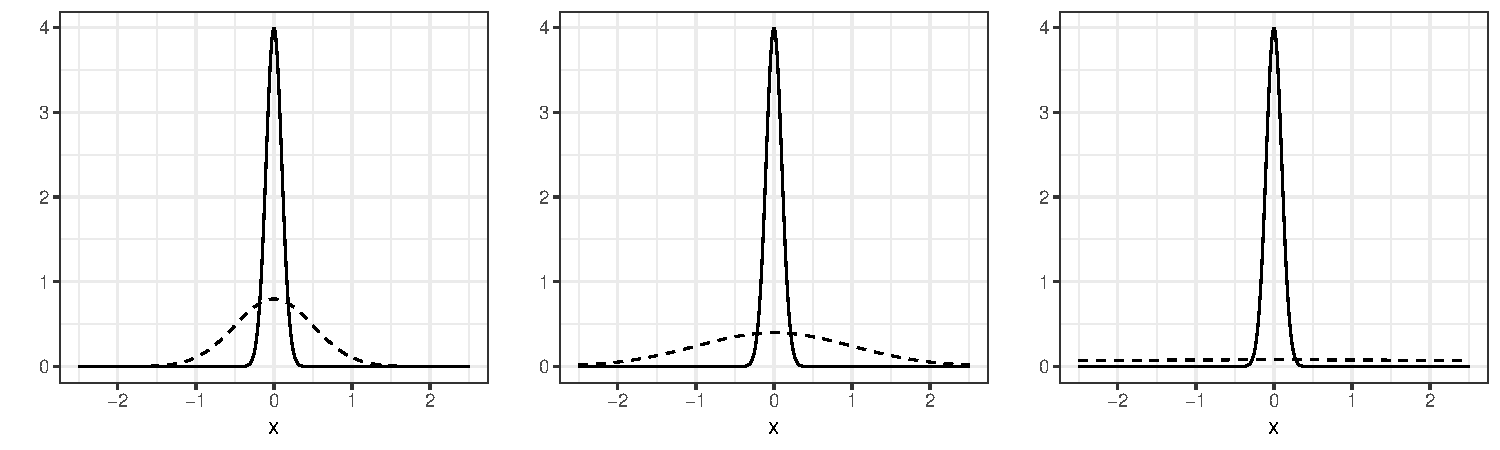
\includegraphics{Dynamic-Shrinkage-in-Bayesian-Structural-Time-Series-and-Vector-Autoregressive-Models_files/figure-latex/myfig1-1} 

}

\caption{Spike (solid line) and Slab (dashed line) distributions with hyperparameters: $\lambda=0.1$ and $c = 5, 10, 50$.}\label{fig:myfig1}
\end{figure}

Equation (\ref{eq:eq2ssvs}) gives the conditional distribution of
\(\beta_j\); the joint conditional distribution of \(\beta_j\) can be
rewritten in a general multivariate form as
\begin{equation*} \label{eq:ssvsmulti}
\boldsymbol{\beta}|\boldsymbol{\gamma}\sim\mathcal{N}(\boldsymbol{0},\boldsymbol{D}_{\gamma}\boldsymbol{R}_{\gamma},\boldsymbol{D}_{\gamma})
\end{equation*} where
\(\boldsymbol{D}_{\gamma} \equiv diag(\alpha_{1}\lambda_{1},...,\alpha_{p}\lambda_{p})\)
with \(\alpha_{j}=1\) if \(\gamma_{j}=0\) and \(\alpha_{j}=c_{j}\) if
\(\gamma_{j}=1\), and \(\boldsymbol{R}_{\gamma}\) is prior correlation
matrix when the model is characterized by gamma. A convenient
specification for the latter is
\(\boldsymbol{R}_{\gamma}=\boldsymbol{I}\) if the \(\beta_j\) can be
considered independent or the
\protect\hyperlink{ref-zellner_1986}{Zellner}
(\protect\hyperlink{ref-zellner_1986}{1986}) \emph{g-prior} that assumes
\(\boldsymbol{R}_{\gamma}^{-1}=g(\boldsymbol{X}'\boldsymbol{X})/n\).
Regarding the priors on the residual variance \(\sigma^{2}\) and on
\(\boldsymbol{\gamma}\), it is reasonable to assume that \(\sigma^2\)
would decrease when the number of active coefficient increases. Thus,
the parameters of the Inverse-Gamma distribution in equation
(\ref{eq:ssvs2.3}) can be set in function of the expected
dimensionality. For instance, interpreting \(n_\gamma\) as the prior
sample size and \(d_\gamma/(n_\gamma-1)\) as the prior estimate of
\(\sigma^2\). One may let \(d_\gamma/(n_\gamma-1)\) be a decreasing
function of \(|\boldsymbol{\gamma}|\). Finally,
\protect\hyperlink{ref-GM_1993}{George and McCulloch}
(\protect\hyperlink{ref-GM_1993}{1993}) recognize the difficulty in
choosing an informative prior for \(\boldsymbol{\gamma}\) especially
when \(p\) is large, thus they suggest the following specification which
assumes independent indicators marginally distributed as in equation
(\ref{eq:ssvs3}), \begin{equation*}
\pi(\boldsymbol{\gamma})=\prod_{j=1}^{p}\omega_{j}^{\gamma_{j}}(1-\omega_{j})^{1-\gamma_{j}}
\end{equation*} This prior basically implies that the inclusion
probability of each regressor is independent of the inclusion of the
others. Despite its simplicity, this prior choice is very effective
since it facilitates Gibbs sampling;
\protect\hyperlink{ref-GM_1993}{George and McCulloch}
(\protect\hyperlink{ref-GM_1993}{1993}) found it to work well in various
situations. Note also that, considering an equal probability of each
regressor to enter the model and thus setting
\(\omega_{j}=\frac{1}{2}\), the prior becomes a uniform
\(\pi(\boldsymbol{\gamma})\equiv 2^{-p}\).\\
Obviously, the priors must be chosen with care, and they must strike a
balance between reliability and functionality. The prior distributions
in SSVS are precisely configured to produce closed form full conditional
distributions, allowing for rapid and efficient simulations using Gibbs
sampling, for example.\\
Alternatively to equation (\ref{eq:ssvsmulti}),
\protect\hyperlink{ref-GM_1997}{George and McCulloch}
(\protect\hyperlink{ref-GM_1997}{1997}) propose a conjugate design for
\((\boldsymbol{\beta},\sigma^{2})\),
i.e.~\(\boldsymbol{\beta}|\sigma^{2},\boldsymbol{\gamma}\sim\mathcal{N}(\boldsymbol{0},\sigma^{2}\boldsymbol{D}_{\gamma}\boldsymbol{R}_{\gamma},\boldsymbol{D}_{\gamma})\).
This formulation simplifies analytical calculations since
\((\boldsymbol{\beta},\sigma^{2})\) can be integrated out from the full
posterior
\(\pi(\boldsymbol{\beta},\sigma^{2},\boldsymbol{\gamma}|y_{1:T})\) and
thus it enables to easily obtain the posterior
\(\pi(\boldsymbol{\gamma}|y_{1:T})\), which is known up to a
proportionality constant, and it can be carried analytically for small
\(p\) or numerically otherwise with MCMC methods.
\protect\hyperlink{ref-GM_1997}{George and McCulloch}
(\protect\hyperlink{ref-GM_1997}{1997}) show that this conjugate design
facilitates MCMC exploration.

\subsection{Bayesian Regularization}

Rather than using auxiliary variables to generate spike and slab
densities, shrinking towards zero can alternatively be achieved by
directly assigning a continuous prior density to the model's parameters.
Such priors are usually exponential density priors of the form
\(\pi(\beta_{j}|\lambda_{j})\propto\exp(-\lambda_{j}|\beta_{j}|^{i})\),
with \(i>0\) and where \(\lambda_{j}\) is a function of the scale
parameter. For example, \protect\hyperlink{ref-T_1996}{Tibshirani}
(\protect\hyperlink{ref-T_1996}{1996}) uses a double-exponential
(Laplace) prior with \(i=1\) and assumes that the regression
coefficients are i.i.d. distributed according to
\[\pi(\beta_{j}|\lambda)=\frac{\lambda}{2}\exp(-\lambda|\beta_{j}|)\]
for \(j=1,...,p\). Assuming a Laplace rather than a Normal distribution
has the effect of increasing the probability mass around zero, resulting
in a more severe shrinking towards zero.
\protect\hyperlink{ref-T_1996}{Tibshirani}
(\protect\hyperlink{ref-T_1996}{1996}) reconciles this Bayesian approach
to variable selection with the frequentist LASSO by showing that the
latter can be regarded as the mode of the posterior distribution of
\(\beta\). However, while in the frequentist LASSO the regression
coefficients are obtained by solving a constrained optimization problem,
in the Bayesian version we rely on simulation algorithms, primarily
MCMC, approximating the posterior distribution which is usually
analytically intractable. This implies that contrary to the frequentist
LASSO that produces sparse models by forcing coefficients to zero, in
the Bayesian LASSO the point estimates are never exactly equal to
zero.\\
The approach of \protect\hyperlink{ref-T_1996}{Tibshirani}
(\protect\hyperlink{ref-T_1996}{1996}) was interestingly developed into
the Bayesian LASSO by \protect\hyperlink{ref-PC_2008}{Park and Casella}
(\protect\hyperlink{ref-PC_2008}{2008}). In this case the regression
coefficients are modeled with a conditional Laplace prior distribution
of the type
\[\pi(\boldsymbol{\beta}|\sigma^{2})=\prod_{j=1}^{p}\frac{\lambda}{2\sqrt{\sigma^2}}\exp\bigg(-\frac{\lambda|\beta_{j}|}{\sqrt{\sigma^2}}\bigg)\]
with an improper density \(\pi(\sigma^{2})\propto \frac{1}{\sigma^{2}}\)
on the variance or an Inverse-Gamma prior that maintains the conjugacy.
The effect of conditioning on \(\sigma^2\) has significant consequences
in terms of convergence of the MCMC strategy and more meaningful point
estimates since it guarantees an unimodal full posterior density.
Interestingly (\protect\hyperlink{ref-AM_1974}{Andrews and Mallows
1974}), a scale mixture of Normal densities with an exponential mixing
density can be used to represent the Laplace distribution: \[
\frac{\lambda}{2}\exp(-\lambda|\beta|)=\int_0^\infty \frac{1}{\sqrt{2\pi s}}\exp\bigg(-\frac{\beta^2}{2s}\bigg)\frac{\lambda}{2}\exp\bigg(-\frac{\lambda^2\beta}{2}\bigg)ds
\] Therefore, the full model can be represented with this hierarchical
scheme \begin{align*}
\boldsymbol{\beta}|\sigma^{2},\tau^{2}_{1},...,\tau^{2}_{p}\sim & \mathcal{N}(\boldsymbol{0},\sigma^{2}\boldsymbol{D}_{\tau}), \\
\boldsymbol{D}_{\tau}= & diag(\tau_{1}^{2},...,\tau_{p}^{2}),\\
\sigma^{2},\tau^{2}_{1},...,\tau^{2}_{p}\sim &  \pi(\sigma^{2})\prod_{j=1}^{p}\frac{\lambda^{2}}{2}\exp\bigg(-\lambda^{2}\tau^{2}_{j}/2\bigg),\\
\sigma^{2},\tau^{2}_{1},...,\tau^{2}_{p}> & 0
\end{align*} which can be simplified by assuming
\(\tau^{2}_{1},...,\tau^{2}_{p}=\tau^{2}\). The Bayesian LASSO
parameter, \(\lambda\), can be estimated in several ways;
\protect\hyperlink{ref-PC_2008}{Park and Casella}
(\protect\hyperlink{ref-PC_2008}{2008}) suggest empirical Bayes via
marginal maximum likelihood or the use of hyperpriors. We refer to the
original article for further details.

\subsection{Reversible Jump MCMC}

The approaches mentioned so far presume that the collection of
predictors is fixed and that individual coefficients are given shrinkage
priors. Alternatively, one can wonder if the number of explanatory
variables in the model is appropriate, or if it is too high or too low.
The Bayesian way to model such uncertainty is straightforward and it
consists of treating also \(N_{p}\) as a random variable and assigning a
prior to it. In this way the degree of sparseness depends on two
factors: the coefficients shrunk towards zero and the dimension of the
regression matrix. The computational challenges of this approach can be
addressed by using reversible jump MCMC algorithms
(\protect\hyperlink{ref-G_1995}{Green}
(\protect\hyperlink{ref-G_1995}{1995})) which allow to simultaneously
explore spaces of different dimensions. The idea is to generate a Markov
Chain in order to simulate from
\(\pi(\boldsymbol{\beta}_{\gamma},\boldsymbol{\gamma}|y_{1:T},\boldsymbol{X})\propto\pi(y_{1:T}|\boldsymbol{X},\boldsymbol{\beta})\pi(\boldsymbol{\beta}|\boldsymbol{\gamma})\pi(\boldsymbol{\gamma})\).
This is commonly achieved through a Metropolis-Hastings algorithm. The
difficulty stands in the fact that in order to explore different spaces
we need a strategy that allow the transition from state
\((\boldsymbol{\beta}_{\gamma},\boldsymbol{\gamma})\) to the state
\((\boldsymbol{\beta}_{\gamma}^{*},\boldsymbol{\gamma}^{*})\) where
\(N_{p} \neq N_{p^*}\). Such ``jump'' from one dimension to an other is
possible through the concept of \emph{dimension matching}. The idea is
the following. Let's say for instance that the jump occurs from
\((\boldsymbol{\beta}_{\gamma},\boldsymbol{\gamma})\) to
\((\boldsymbol{\beta}_{\gamma^{*}}^{*},\boldsymbol{\gamma}^{*})\) where
\(N_{p}<N_{p*}\). To make this jump possible a random vector
\(\boldsymbol{u}\) with density
\(h_{\gamma \to \gamma^*}(\boldsymbol{u})\) and length
\((N_{p^*}-N_{p})\) is generated from a known density. The aim of this
vector is to fill the dimensional gap between \(\boldsymbol{\gamma}\)
and \(\boldsymbol{\gamma}^{*}\). In other words, considering a
one-to-one mapping function
\(g_{\gamma \to \gamma^*}:\mathbb{R}^{N_{p}}\times\mathbb{R}^{N_{p^*}-N_{p}}\to\mathbb{R}^{N_{p^*}}\),
the relationship between the current and the new state is given by
\(\boldsymbol{\beta}^{*}_{\gamma^{*}}=g_{\gamma \to \gamma^*}(\boldsymbol{\beta}_{\gamma},\boldsymbol{u})\).
Once we generate a random candidate state
\((\boldsymbol{\beta}_{\gamma}^{*},\boldsymbol{\gamma}^{*})\), its
acceptance probability must take into account also the change in
dimensions, thus it is necessary to compute the Jacobian of \(g\):
\begin{equation*}\label{eq:jumpMCMC}
\alpha((\boldsymbol{\beta}_{\gamma},\boldsymbol{\gamma}),(\boldsymbol{\beta}_{\gamma}^{*},\boldsymbol{\gamma}^{*}))=\min\bigg\{1,\frac{\pi(\boldsymbol{\beta}_{\gamma}^{*},\boldsymbol{\gamma}^{*}|y_{1:T},\boldsymbol{X})q(\boldsymbol{\gamma}^{*}\to\boldsymbol{\gamma})}{\pi(\boldsymbol{\beta}_{\gamma},\boldsymbol{\gamma}|y_{1:T},\boldsymbol{X})q(\boldsymbol{\gamma} \to\boldsymbol{\gamma}^{*})h_{\gamma\to\gamma^{*}}(\boldsymbol{u})}\bigg|\frac{\partial g_{\gamma\to\gamma^{*}}(\boldsymbol{\beta}_{\gamma},\boldsymbol{u})}{\partial (\boldsymbol{\beta}_{\gamma},\boldsymbol{u})}\bigg|\bigg\}
\end{equation*}

where \(q(\boldsymbol{\gamma}^* \to \boldsymbol{\gamma})\) is the the
probability of proposing a transaction from
\((\boldsymbol{\beta}_{\gamma},\boldsymbol{\gamma})\) to
\((\boldsymbol{\beta}_{\gamma}^{*},\boldsymbol{\gamma}^{*})\). In the
same way, the acceptance ratio of the reverse move proposal (from
\(\boldsymbol{\gamma}^* \to \boldsymbol{\gamma}\)) is given by
\(\alpha((\boldsymbol{\beta}_{\gamma},\boldsymbol{\gamma}),(\boldsymbol{\beta}_{\gamma}^{*},\boldsymbol{\gamma}^{*}))\).
The mechanism just introduced, however, requires a wise evaluation of
the functions \(h\) and \(g\), since their choice could affect the
performances of the simulation strategy.\\
Moreover, one may relax the assumptions on the size of
\(\boldsymbol{u}\). In this case, the dimensionality can still be
matched by letting the length of \(\boldsymbol{u}\) to be equal to
\(l_{p}\) such that \(N_{p}+l_{p}=N_{p^*}+l_{p^*}\). However, now
\(\boldsymbol{u}^{*}\) cannot be generated by the inverse function of
\(h_{\gamma \to \gamma^*}\) since it is no more available in
deterministic terms. Therefore, \(\boldsymbol{u}^*\) will be generated
from a new density \(h_{\gamma^* \to \gamma}=(\boldsymbol{u}^*)\).
Finally, in addition to the mapping
\(\boldsymbol{\beta}^{*}_{\gamma^{*}}=g_{\gamma \to \gamma^*}(\boldsymbol{\beta}_{\gamma},\boldsymbol{u})\)
is added a reverse mapping
\(\boldsymbol{\beta}_{\gamma}=g_{\gamma^*\to\gamma}(\boldsymbol{\beta}^{*}_{\gamma^*},\boldsymbol{u}^*)\).
The new acceptance probability is thus
\begin{equation*}\label{eq:jumpMCMC1}
\alpha((\boldsymbol{\beta}_{\gamma},\boldsymbol{\gamma}),(\boldsymbol{\beta}_{\gamma}^{*},\boldsymbol{\gamma}^{*}))=\min\bigg\{1,\frac{\pi(\boldsymbol{\beta}_{\gamma}^{*},\boldsymbol{\gamma}^{*}|y_{1:T},\boldsymbol{X})q(\boldsymbol{\gamma}^{*}\to\boldsymbol{\gamma})h_{\gamma^{*}\to\gamma}(\boldsymbol{u^*})}{\pi(\boldsymbol{\beta}_{\gamma},\boldsymbol{\gamma}|y_{1:T},\boldsymbol{X})q(\boldsymbol{\gamma} \to\boldsymbol{\gamma}^{*})h_{\gamma\to\gamma^{*}}(\boldsymbol{u})}\bigg|\frac{\partial g_{\gamma\to\gamma^{*}}(\boldsymbol{\beta}_{\gamma},\boldsymbol{u})}{\partial (\boldsymbol{\beta}_{\gamma},\boldsymbol{u})}\bigg|\bigg\}.
\end{equation*}

In general, Reversible Jump MCMC have proved to perform well for
variable selection and they allow for a rapid mixing time. However, we
do not explore this approach further. See
\protect\hyperlink{ref-G_1995}{Green}
(\protect\hyperlink{ref-G_1995}{1995}) for furthers details and
examples.

\section{Bayesian Structural Time Series} \label{Bayesian Structural Time Series}

After \protect\hyperlink{ref-varian_choi_2009}{Varian and Choi}
(\protect\hyperlink{ref-varian_choi_2009}{2009a}), the awareness of
scientists about the effectiveness of web data (and in particular Google
Trends) in improving forecasting increased. However, because of the high
dimensionality, dealing with such great amount of data poses new
modelling challenges. In order to meet the demand for an ensemble method
able to average over different combinations of predictors in time series
analysis, Steven L. Scott and Hal Varian, respectively Senior Economist
Analyst and Chief Economist at Google Inc, developed a new methodology
that combines State-Space Models and Bayesian Variable Selection
Methods. The authors refer to this new class of models as
\emph{Bayesian Structural Time Series} (BSTS). The latter is based on
three pillars:

\begin{itemize}
\itemsep-0.5em 
  \item Structural Time Series Models
  \item Spike and Slab Regression
  \item Markov Chain Monte Carlo methods
\end{itemize}

We develop the discussion in the next three sections.

\subsection{Structural Time Series Models}\label{Structural Time Series Models}

Structural Time Series Models can be regarded as a subclass of Dynamic
Linear Models (DLM) where the state process describes the evolution of
some unobserved time series features, precisely the trend, the seasonal
and, possibly, the cycle components. Intuitively, they remind of the
classical time series decomposition, that describes a time series as
composed by some systematic components (trend, seasonality, cycle) and a
random component (noise). However, while classical decomposition is just
a descriptive tool, Structural Time Series Models are probabilistic
models, and allow prediction and a proper quantification of uncertainty
- assuming that we are able to identify the components from the noisy
background. Formulating the problem in the form of general multivariate
DLM, the observable \(\mathbb{R}^{n}\)-valued time series
\((\boldsymbol{Y}_{t})_{t\geq 1}\) is related to the latent
\(\mathbb{R}^{p}\)-valued state process
\((\boldsymbol{\theta}_{t})_{t\geq 0}\) through the following system of
equation, for each \(t\geq1\), \begin{align} \label{eq:DLM1}
\boldsymbol{Y}_{t} = & \boldsymbol{F}_{t}\boldsymbol{\theta}_{t}+\boldsymbol{\epsilon}_{t}, \ \ \ \boldsymbol{\epsilon}_{t}\sim\mathcal{N}_{n}(\boldsymbol{0},\Sigma_{\epsilon,t}) \\
\boldsymbol{\theta}_{t} = & \boldsymbol{G}_{t}\boldsymbol{\theta}_{t-1}+\boldsymbol{\eta}_{t}, \ \ \ \boldsymbol{\eta}_{t}\sim\mathcal{N}_{p}(\boldsymbol{0},\Sigma_{\eta,t}) \label{eq:DLM2}
\end{align} with
\(\boldsymbol{\theta}_{0}\sim\mathcal{N}_{p}(\boldsymbol{m}_{0},\boldsymbol{C}_{0})\).
\(\boldsymbol{F}_{t}\) and \(\boldsymbol{G}_{t}\) are respectively a
\(n \times p\) and a \(p \times p\). The disturbances,
\((\boldsymbol{\epsilon}_{t})\) and \((\boldsymbol{\eta}_{t})\), are
assumed to be two sequences of serially uncorrelated Gaussian random
vectors with mean zero and \(p \times p\) covariance matrices
\(\Sigma_{\epsilon,t}\) and \(\Sigma_{\eta,t}\). Moreover,it is assumed
that
\((\boldsymbol{\epsilon}_{t}) \perp\!\!\!\perp (\boldsymbol{\eta}_{t})\perp\!\!\!\perp \boldsymbol{\theta}_{0}\).
Equation (\ref{eq:DLM1}) s refereed to as the observation equation and
equation (\ref{eq:DLM2}) as the state equation. State-space models
naturally arise in problems of fintering, where interest is in
extracting the signal, \((\boldsymbol{\theta}_{t})_{t \geq 1}\), from an
incomplete, potentially noisy, set of observations
\((\boldsymbol{y}_{t})_{t\geq 1}\). Very briefly, this is possible
through a recursive procedure that exploits the Markovian structure of
the state process and the assumption of conditionally independent
observations (see (A.1) and (A.2)) in order to compute the filter and
predictive densities at any time \(t\) starting from
\(\boldsymbol{\theta}_{0}\sim p_{0}\). The process of filtering can be
summarized in three steps. Let
\((\boldsymbol{Y}_{t},\boldsymbol{\theta}_{t})_{t \geq 1}\) be a
discrete time stochastic process satisfying (A.1) and (A.2), and
\(\boldsymbol{\psi}\) a vector of model's parameters, for \(t\geq 1\)
compute

\begin{enumerate}[label=(\roman*)]
\item The one-step-ahead predictive distribution for the states using the filtering density at time $t-1$, $\pi(\boldsymbol{\theta}_{t-1}|\boldsymbol{y}_{1:t-1})$: \[\pi(\boldsymbol{\theta}_{t}| \boldsymbol{y}_{1:t-1})=\int\int \pi(\boldsymbol{\theta}_{t}|\boldsymbol{\theta}_{t-1},\boldsymbol{\psi}) \pi(\boldsymbol{\theta}_{t-1}|\boldsymbol{y}_{1:t-1},\boldsymbol{\psi})\pi(\boldsymbol{\psi}|\boldsymbol{y}_{1:t-1}) \ d\boldsymbol{\theta}_{t-1}\ d\boldsymbol{\psi} \]
\item The one-step-ahead predictive distribution for the observations using the density computed in step (i): \[\pi(\boldsymbol{y}_{t}|\boldsymbol{y}_{1:t-1})=\int\int \pi(\boldsymbol{y}_{t}|\boldsymbol{\theta}_{t},\boldsymbol{\psi}) \pi(\boldsymbol{\theta}_{t}|\boldsymbol{y}_{1:t-1},\boldsymbol{\psi})\pi(\boldsymbol{\psi}|\boldsymbol{y}_{1:t-1})  \ d\boldsymbol{\theta_{t}}\  d\boldsymbol{\psi}\]
\item The filtered distribution at time $t$ using the densities computed at step(i) and step (ii):  \[\pi(\boldsymbol{\theta}_{t}|\boldsymbol{y}_{1:t})=\frac{\pi(\boldsymbol{y}_{t}|\boldsymbol{\theta}_{t})\pi(\boldsymbol{\theta}_{t}|\boldsymbol{y}_{1:t-1})}{\pi(\boldsymbol{y}_{t}|\boldsymbol{y}_{1:t-1})}\]
\end{enumerate}

Such densities are available in closed form and they are easy to compute
in linear Gaussian State-Space Models only when model's parameters are
known. In this latter case, the joint distribution for
\((\boldsymbol{\theta}_{0},\boldsymbol{\theta}_{1},...,\boldsymbol{\theta}_{T},\boldsymbol{Y}_{1},...,\boldsymbol{Y}_{T})\)
is a multivariate Normal distribution, which implies that also the
marginal and conditional distributions are normally distributed.
Therefore they are characterized by the first two moments, which are
obtained by the celebrated Kalman Filter which is based on the process
described below. Let
\(\boldsymbol{\theta}_{0}\sim \mathcal{N}(\boldsymbol{m}_{0},\boldsymbol{C}_{0})\),
compute for \(t=1,...,T\) \begin{equation}\label{eq:Kalman}
\begin{matrix}
\boldsymbol{a}_{t}=\mathbb E(\boldsymbol{\theta}_{t}|\boldsymbol{y}_{1:t-1})=\boldsymbol{G}_{t}\boldsymbol{m}_{t-1}, & \boldsymbol{R}_{t}=\mathbb V(\boldsymbol{\theta}_{t}|\boldsymbol{y}_{1:t-1})=\boldsymbol{G}_{t}\boldsymbol{C}_{t-1}\boldsymbol{G}_{t}'+\Sigma_{\eta,t}, \\
\boldsymbol{f}_{t}=\mathbb E(\boldsymbol{y}_{t}|\boldsymbol{y}_{1:t-1})=\boldsymbol{F}_{t}\boldsymbol{a}_{t}, & \boldsymbol{Q}_{t}=\mathbb V(\boldsymbol{y}_{t}|\boldsymbol{y}_{1:t-1})=\boldsymbol{F}_{t}\boldsymbol{R}_{t}\boldsymbol{F}_{t}'+\Sigma_{\epsilon,t}, \\
\boldsymbol{m}_{t}=\mathbb E(\boldsymbol{\theta}_{t}|\boldsymbol{y}_{1:t})=\boldsymbol{a}_{t}+\boldsymbol{A}_{t}\boldsymbol{e}_{t}, & \boldsymbol{C}_{t}=\mathbb V(\boldsymbol{\theta}_{t}|\boldsymbol{y}_{1:t})=\boldsymbol{R}_{t}-\boldsymbol{A}_{t}\boldsymbol{Q}_{t}\boldsymbol{A}_{t}' \\
\end{matrix}
\end{equation} where
\(\boldsymbol{A}_{t}=\boldsymbol{R}_{t}\boldsymbol{F}_{t}'\boldsymbol{Q}_{t}^{-1}\)
and \(\boldsymbol{e}_{t}=\boldsymbol{y}_{t}-\boldsymbol{f_t}\). The
problem of smoothing, that is, the computation of the distribution of
\(\boldsymbol{\theta}_{0:T} \mid \boldsymbol{y}_{1:T}\) is similarly
solved by Kalman smoothing. Given the filtering distribution at time
\(T\), we trace the states' history up T through backward recursive
formulae. Let
\(\boldsymbol{\theta}_{t+1}|\boldsymbol{y}_{1:T}\sim\mathcal{N}(\boldsymbol{s}_{t+1},\boldsymbol{S}_{t+1})\),
then
\(\boldsymbol{\theta}_{t}|\boldsymbol{y}_{1:T}\sim\mathcal{N}(\boldsymbol{s}_{t},\boldsymbol{S}_{t})\)
\begin{equation}\label{eq:Smooth}
\begin{matrix}
\boldsymbol{s}_{t}={m}_{t}+\boldsymbol{B}_{t}(\boldsymbol{s}_{t+1}-\boldsymbol{a}_{t+1}), & \boldsymbol{S}_{t}=\boldsymbol{C}_{t}-\boldsymbol{B}_{t}(\boldsymbol{R}_{t+1}-\boldsymbol{S}_{t+1})\boldsymbol{B}_{t}'
\end{matrix}
\end{equation} where
\(\boldsymbol{B}_{t}=\boldsymbol{C}_{t}\boldsymbol{G}_{t+1}'\boldsymbol{R}_{t+1}^{-1}\).
Jointly, Kalman Filter (also known as \emph{forward step}) and Kalman
Smoother (or \emph{backward step}) provide the posterior distribution of
the states assuming that the matrices of the model are known.
Unfortunately, the model's parameters are usually unknown. Nevertheless,
the process described in (\ref{eq:Kalman}) and (\ref{eq:Smooth}) to
obtain moments can be used in Markov Chain Monte Carlo methods to
compute the full conditional distribution
\(p(\boldsymbol{\theta}_{t}|\boldsymbol{y}_{1:t},\boldsymbol{\psi})\).
Further details on MCMC are provided in Section
\ref{MCMC methods for posterior inference}.\\
Let us now consider the BSTS model's specification. We restrict our
attention to univariate time series, as in
\protect\hyperlink{ref-scott_varian_2013}{Scott and Varian}
(\protect\hyperlink{ref-scott_varian_2013}{2013}), but multivariate
extensions are available (see \protect\hyperlink{ref-ning2021mbsts}{Ning
and Qiu} (\protect\hyperlink{ref-ning2021mbsts}{2021})). As already
mentioned, the time series structural components enter the model through
the state vector or, in other words,
\(\boldsymbol{\theta}_{t}=(\mu_{t},\delta_{t},\tau_{t})'\) where
\(\mu_{t}\) is the level of the series at time \(t\), \(\delta_{t}\) is
its the time-varying growth and \(\tau_{t}\) is the seasonal factor. A
convenient way to deal with seasonality is to consider the seasonal
factors as the dynamic coefficients of a set of \(S\) dummy variables
and constrain them to have zero expectation over a full cycle of \(S\)
seasons. Finally, augmenting the observation equation with a regression
component, we obtain a Bayesian Structural Time Series model
\begin{align} \label{eq:eqbsts}
  Y_{t} & =\mu_{t}+\tau_{t}+\boldsymbol{x}'_{t}\boldsymbol{\beta}+\epsilon_{t}\\
  \mu_{t} & = \mu_{t-1}+\delta_{t-1}+u_{t} \nonumber \\
  \delta_{t} & = \delta_{t-1}+v_{t} \nonumber \\
  \tau_{t} & =-\sum_{s=1}^{S-1}\tau_{t-s}+w_{t} \nonumber
  \end{align} With reference to equation (\ref{eq:DLM2}),
\(\boldsymbol{\eta}_{t}=(u_{t},v_{t},w_{t})'\) and
\(\boldsymbol{\eta}_{t} \sim N_{3}(\boldsymbol{0},\Sigma_{\eta})\) where
\(\Sigma_{\eta,t}=diag(\sigma^{2}_{u},\sigma^{2}_{v},\sigma^{2}_{w})\),
while \(\Sigma_{\epsilon,t}=\sigma^{2}_{\epsilon}\) in equation
(\ref{eq:DLM1}), for \(t \geq 1\). The unknown parameters of this model
are
\((\boldsymbol{\beta},\sigma^{2}_{\epsilon},\sigma^{2}_{u},\sigma^{2}_{v},\sigma^{2}_{w})\).
We assign a prior to the unknown parameters, that is updated as new
observations become available. More insights on this are provided in
Section \ref{MCMC methods for posterior inference}. In the next
paragraph (Section
\ref{Static Shrinkage in Bayesian Structural Time Series}) we focus
instead on the regression part and the problem of Bayesian variable
selection.

\subsection{Static Shrinkage in Bayesian Structural Time Series}\label{Static Shrinkage in Bayesian Structural Time Series}

A static regression component is frequently included in Bayesian
Structural Time Series. The latter can be incorporated into the baseline
state space model in a variety of ways. The method envisaged by
\protect\hyperlink{ref-scott_varian_2013}{Scott and Varian}
(\protect\hyperlink{ref-scott_varian_2013}{2013}) is conceptually the
simplest and operationally the most efficient. It consists in appending
a constant \(1\) to the state vector \(\boldsymbol{\theta}_{t}\) and
\(\boldsymbol{x}'_{t}\boldsymbol{\beta}\) to \(Z_{t}\) in equation
(\ref{eq:eqbsts}). In this way the dimension of the state vector
increases just by one, regardless the number of predictors, and since
the computational complexity of the Kalman filter is linear in the
length of the data and quadratic in the dimension of the state vector,
the computational savings are substantial. Considering that BSTS have
been developed to deal with internet data, the number of predictors
entering our model might be potentially huge and, in particular, much
larger than the number of available observations (in other words
\(p>>T\)). Therefore, estimation issues are likely to arise. To cope
with this, spike-and-slab regression is used to introduce sparsity among
the regression coefficients. Especially when using web data, it is
indeed safe to assume that many predictors would not play any role in
the regression and thus they must be shrunk to zero. For this purpose,
\protect\hyperlink{ref-scott_varian_2013}{Scott and Varian}
(\protect\hyperlink{ref-scott_varian_2013}{2013}) rely on the SSVS we
discussed in Section \ref{Indicator Model Selection}. Let \(\gamma_{j}\)
be an auxiliary binary indicator assuming two values \begin{align*}
\gamma_{j} & = 1 \ \ \ \text{if} \ \ \ \beta_{j} \neq 0 \\
\gamma_{j} & = 0  \ \ \ \text{if} \ \ \ \beta_{j}=0
\end{align*} where \(\beta_{j}\) is the coefficient of the \(j\)-th
predictor. Let \(\boldsymbol\beta_{\gamma}\) be the subset of active
coefficients, i.e \(\beta_{j} \neq 0\). A spike-and-slab prior can be
written \begin{equation*}
\pi(\boldsymbol{\beta},\boldsymbol{\gamma},\sigma^{2}_{\epsilon})=\pi(\boldsymbol{\beta}_{\gamma}|\boldsymbol{\gamma},\sigma^{2}_{\epsilon})\pi(\sigma^{2}_{\epsilon}|\boldsymbol{\gamma})\pi(\boldsymbol{\gamma})
\end{equation*} where \(\pi(\boldsymbol{\gamma})\) is the spike and, in
practice, it usually coincides with a Bernoulli prior \begin{equation*}
\boldsymbol{\gamma }\sim \prod_{j=1}^{p}\pi_{j}^{\gamma_{j}}(1-\pi_{j})^{1-\gamma_{j}}
\end{equation*} which can be simplified by assuming that the probability
of the indicator to be \(0\) or \(1\) is the same for each predictor or,
in other words, by imposing \(\pi_{j}=\pi\). Moreover, there are
multiple ways to set the hyperparameter's values. Coherently with the
Bayesian approach, a simple strategy is to fix \(\pi\) according to the
``expected model size.'' Therefore the idea is to make a guess on how
many coefficients we expect to be active, \(p_{0}\), and then set
\(\pi=\frac{p_{0}}{p}\). On the other hand, a convenient way to model
\(\boldsymbol{\beta}\) and \(\sigma^{2}_{\epsilon}\) is through a
conjugate prior law, namely the Normal-Gamma prior distribution
\begin{align} \label{eq:bsts2}
\boldsymbol{\beta}_{\gamma}|\boldsymbol{\gamma},\sigma^{2}_{\epsilon} & \sim \mathcal{N}(\boldsymbol{b}_{\gamma},\sigma^{2}_{\epsilon}(\Omega_{\gamma}^{-1})^{-1}) \\
\frac{1}{\sigma_{\epsilon}^{2}}|\boldsymbol{\gamma }& \sim \mathcal{G}\bigg(\frac{n_{0}}{2},\frac{d_{0}}{2}\bigg)  \label{eq:bsts3}
\end{align} where \(\boldsymbol{b}_{\gamma}\) is a vector of prior
guesses for non null predictors, \(\Omega\) is a symmetric matrix and
\(\Omega_{\gamma}\) denote the rows and columns of \(\Omega\) for which
\(\gamma_{j}=1\). Furthermore, \(n_{0}\) represents the prior sample
size and \(d_{0}\) is the prior sum of squares. They can be set properly
by making a guess on the number of observations worth of weight and the
expected \(R^{2}\). Therefore, equations (\ref{eq:bsts2}) and
(\ref{eq:bsts3}) represent the slab density, which can be more or less
informative according to how the hyperparameters have been set. Finally,
for effective shrinkage, a possible prior distribution for
\(\boldsymbol{\beta}_{\gamma}|\boldsymbol{\gamma},\sigma^{2}_{\epsilon}\)
is the ``g-prior'' proposed by
\protect\hyperlink{ref-zellner_1986}{Zellner}
(\protect\hyperlink{ref-zellner_1986}{1986}). The latter is
characterized by a null vector \(\boldsymbol{b}_{\gamma}\) and
\(\Omega^{-1}=g\boldsymbol{X}'\boldsymbol{X}/n\).\\
Let
\(y^{\star}_{t}=y_{t}-\boldsymbol{F}_{t}^{\star}\boldsymbol{\theta}_{t}\)
where \(\boldsymbol{F}_{t}^{\star}\) is the observation matrix of
equation (\ref{eq:DLM1}) with the regression component
\(\boldsymbol{\beta}'\boldsymbol{x}_{t}\) set to zero and let
\(y_{1:T}^{\star}=(y_{1}^{\star},...,y_{t}^{\star})\). Thanks to the
conjugate nature of the model, posterior inference can be carried out.
The Bayesian updating process of a Normal-Gamma prior leads to a
Normal-Gamma posterior distribution with parameters: \begin{align*}
\boldsymbol{\beta}_{\gamma}|\boldsymbol{\gamma},\sigma^{2}_{\epsilon},y_{1:T}^{\star} & \sim \mathcal{N}( \tilde{\boldsymbol{\beta}}_{\gamma},\sigma^{2}_{\epsilon}(\Lambda_{\gamma}^{-1})^{-1}) \\
\frac{1}{\sigma_{\epsilon}^{2}}|\boldsymbol{\gamma},y_{1:T}^{\star} & \sim \mathcal{G}\bigg(\frac{n_T}{2},\frac{d_T}{2}\bigg)
\end{align*} where \begin{align*}
\Lambda_{\gamma}^{-1} & =(\boldsymbol{X}'\boldsymbol{X})_{\gamma}+\Omega_{\gamma}^{-1} \\
n_{T} & = n_{0} + T \\
\tilde{\boldsymbol{\beta}_{\gamma}} & =(\Lambda_{\gamma}^{-1})^{-1}(\boldsymbol{X}_{\gamma}'y_{1:T}^{\star}+\Omega_{\gamma}^{-1}\boldsymbol{b}_{\gamma}) \\
d_{T} & =d_{0}+{y_{1:T}^{\star}}' y_{1:T}^{\star}+ \boldsymbol{b}_{\gamma}'\Omega_{\gamma}^{-1}\boldsymbol{b}_{\gamma}-\tilde{\boldsymbol{\beta}_{\gamma}}'\Lambda_{\gamma}^{-1}\tilde{\boldsymbol{\beta}_{\gamma}}
\end{align*} Moreover, it is possible to marginalize out
\(\boldsymbol{\beta}_{\gamma}\) and \(\sigma^{2}_{\epsilon}\) from the
full posterior distribution
\(\pi(\boldsymbol{\beta}_{\gamma},\sigma^{2}_{\epsilon},\boldsymbol{\gamma})\)
and obtain the marginal posterior distribution of the indicator
\begin{equation*}
\boldsymbol{\gamma}|y_{1:T}^{\star} \sim C(y_{1:T}^{\star})\frac{|\Omega^{-1}_{\gamma}|^{\frac{1}{2}}\pi(\boldsymbol{\gamma})}{|\Lambda^{-1}_{\gamma}|^{\frac{1}{2}}d_{T}^{\frac{n_{T}}{2}-1}}
\end{equation*} where \(C(y_{1:T}^{\star})\) is a normalizing constant
that depends on \(\boldsymbol{y}^\star\) but not on
\(\boldsymbol{\gamma}\). This equation can be used to draw from the
posterior distribution of every \(\gamma_{j}\) given
\(\boldsymbol{\gamma}_{-j}\), which represents all the elements of
\(\boldsymbol{\gamma}\) except \(\gamma_{j}\). However, the MCMC
algorithms used to fit the model is such that it does not require
\(C(y_{1:T}^{\star})\) to be computed explicitly.

\subsection{MCMC methods for posterior inference}\label{MCMC methods for posterior inference}

Let
\(\boldsymbol{\psi}=(\boldsymbol{\beta},\sigma^{2}_{\epsilon},\sigma^{2}_{u},\sigma^{2}_{v},\sigma^{2}_{w})\)
be the vector of model parameters and \(y_{t+h}\) the \(h\)-step ahead
forecast, the Bayesian approach to parameter learning and forecasting is
based on providing their respective posterior distribution starting from
an assigned prior distribution. The prior densities of
\((\boldsymbol{\beta},\sigma^{2}_{\epsilon})\) have already been
described in the previous paragraph; we also assign an Inverse-Gamma
prior to \((\sigma^{2}_{u},\sigma^{2}_{v},\sigma^{2}_{w})\) so that the
update rule is analytically available. Since model's parameters are
unknown, and here treated as random quantities, Kalman Filter and Kalman
Smoother cannot be directly used to obtain a full description of these
densities, but an approximate solution can be obtained through Markov
Chain Monte Carlo (MCMC) methods. The algorithm below is the Gibbs
sampling presented in \protect\hyperlink{ref-scott_varian_2013}{Scott
and Varian} (\protect\hyperlink{ref-scott_varian_2013}{2013}).

\begin{algorithm}
\caption{Parameter learning in BSTS} \label{alg:BSTS}
\begin{center}
\emph{Step 1: Sample states and States' variances}\\
\end{center}
\nl Sample $\theta_{0:T}$ from $p(\theta_{0:T}|\boldsymbol{\beta},\sigma^{2}_{\epsilon},\Sigma_{\eta},y_{1:T})$ using the method proposed by Durbin and Koopman (2002)\;
\nl Sample indipendently the diagonal elements of $\Sigma_{\eta}$ from $p(\sigma^{2}_{i}|\theta_{0:T},\boldsymbol{\beta},\sigma^{2}_{\epsilon},y_{1:T})$ for $i \in \{u,v,w\}$\;
\begin{center}
\emph{Step 2: SSVS}\\
\end{center}
\nl Sample the coefficient vector $\boldsymbol{\beta}$ from $p(\boldsymbol{\beta}|\theta_{0:T},\sigma^{2}_{\epsilon},\boldsymbol{\gamma},y_{1:T})$\;
\nl Sample $\sigma^{2}_{\epsilon}$ from $p(\sigma^{2}_{\epsilon}|\theta_{0:T},\boldsymbol{\beta},\boldsymbol{\gamma},y_{1:T})$\;
\nl Sample the indicator vector $\boldsymbol\gamma$ componentwise by sampling consecutively from $p(\gamma_{j}|\theta_{0:T},\boldsymbol\beta,\boldsymbol\gamma_{-j},y_{1:T})$
\end{algorithm}

The first step of Algorithm \ref{alg:BSTS} can be carried out in a
variety of way. In \protect\hyperlink{ref-scott_varian_2013}{Scott and
Varian} (\protect\hyperlink{ref-scott_varian_2013}{2013}), the authors
propose the Simulation Smoother developed by
\protect\hyperlink{ref-Durbin_K2002}{Durbin and Koopman}
(\protect\hyperlink{ref-Durbin_K2002}{2002}). A brief description of
this method is reported separately in Algorithm \ref{alg:DK2002}. Some
of the other existing strategies that are used in Chapter
\ref{Dynamic Shrinkage} are the Forward Filter Backward Sampling (FFBS)
algorithm by \protect\hyperlink{ref-CK_1994}{Carter and Kohn}
(\protect\hyperlink{ref-CK_1994}{1994}),
\protect\hyperlink{ref-fruhwirth-schnatter_1994}{Fruhwirth-Schnatter}
(\protect\hyperlink{ref-fruhwirth-schnatter_1994}{1994}),
\protect\hyperlink{ref-S_1994}{Shephard}
(\protect\hyperlink{ref-S_1994}{1994}) and the more recent sparse matrix
method of \protect\hyperlink{ref-chan_jeliazkov_2009}{Chan and
Jeliazkov} (\protect\hyperlink{ref-chan_jeliazkov_2009}{2009}).

\begin{algorithm}
\caption{Simulation Smoother by Durbin and Koopman (2002)} \label{alg:DK2002}
\nl Draw $\boldsymbol{\xi}^{+}\sim \mathcal{N}(\boldsymbol{0},\boldsymbol{\Sigma}_{\xi})$, where $\boldsymbol{\xi}=(\boldsymbol{\epsilon}_{1}',\boldsymbol{\eta}_{1}',...,\boldsymbol{\epsilon}_{T}',\boldsymbol{\eta}_{T}')'$ \\ and $\boldsymbol{\Sigma}_{\xi}=diag(\Sigma_{\epsilon,1},\Sigma_{\eta,1},...,\Sigma_{\epsilon,T},\Sigma_{\eta,T})$ \;
\nl Draw $\boldsymbol{\theta}_{0}\sim\mathcal{N}(\boldsymbol{m}_{0},\boldsymbol{C}_{0})$\;
\nl Compute $\boldsymbol{\theta}^{+}_{t}$ and $\boldsymbol{y}^{+}_{t}$, using equation (\ref{eq:DLM2}) and \ref{eq:DLM1} for $t=1,...,T$\;
\nl Apply Kalman Filter and Kalman Smoother to $\boldsymbol{y}_{1:T}$ and $\boldsymbol{y}_{1:T}^{+}$, respectively the original and the simulated time series, and compute $\boldsymbol{m}_{t}$ and $\boldsymbol{m}_{t}^{+}$ for $t=0,...,T$\;
\nl Compute the mean correction $\tilde{\boldsymbol{\theta}}_{t}$=$\boldsymbol{m}_{t}+(\boldsymbol{\theta}^{+}_{t}-\boldsymbol{m}_{t}^{+})$ for $t=0,...,T$ and obtained the corrected trajectory of the latent states $\tilde{\boldsymbol{\theta}}_{0:T}$\;
\end{algorithm}

Forecasting and parameter learning are two interconnected issue. Let
\(\boldsymbol{\tilde{y}}=(y_{T+1},...,y_{T+h})\) the random vector of
future observations, forecasting coincides with making inference on the
posterior density \(\pi(\boldsymbol{\tilde{y}}|y_{1:T})\). Such
distributions is easy to sample once we have knowledge of the
parameters, by integrating out the latter:
\begin{equation} \label{eq:postforecast}
\pi(\boldsymbol{\tilde{y}}|y_{1:T})=\int_{\Psi} \pi(\boldsymbol{\tilde{y}}|\boldsymbol{\psi},y_{1:T})\pi(\boldsymbol{\psi}|y_{1:T}) \ d\boldsymbol{\psi}
\end{equation} where
\(\pi(\boldsymbol{\tilde{y}}|\boldsymbol{\psi},y_{1:T})\) is obtain
through the following recursion. For \(h=1,2,...\)

\begin{enumerate}[label=(\roman*)]
\item $\pi(\boldsymbol{\theta}_{t+h}|\boldsymbol{\psi},y_{1:T})=\int \pi(\boldsymbol{\theta}_{t+h}|\boldsymbol{\psi},\boldsymbol{\theta}_{t+h-1})\pi(\boldsymbol{\theta}_{t+h-1}|\boldsymbol{\psi},y_{1:T}) d\boldsymbol{\theta}_{t+h-1}$
\item $\pi(y_{t+h}|\boldsymbol{\psi}, y_{1:T})=\int \pi(y_{t+h}|\boldsymbol{\psi},\boldsymbol{\theta}_{t+h})\pi(\boldsymbol{\theta}_{t+k}|\boldsymbol{\psi},y_{1:T}) d\boldsymbol{\theta}_{t+h}$
\end{enumerate}

The draws generated from the density of equation (\ref{eq:postforecast})
can be used to compute quantities of interest such as the expected
values, the median, the variance and the quantiles. Moreover, an
interesting feature of SSVS algorithm is that each draw
\((\boldsymbol{\theta}_{0:T}^{(i)},\boldsymbol{\psi}^{(i)})\),
\(i=1,...,N\), where \(N\) is the number of draws, depends on a
different \(\boldsymbol{\gamma}^{(i)}\) or, in other words, on a
different model. Therefore the posterior predictive distribution can be
thought as a weighted average of model-specific predictive distributions
where the weights are given by \(\pi(\boldsymbol{\gamma}|y_{1:T})\).
This mechanism is better known as Bayesian Model Averaging.\\
Finally, the intrinsic flexibility of Bayesian Structural Time Series
models allows to insert a dynamic regression component into the system
of equation (\ref{eq:eqbsts}). Although
\protect\hyperlink{ref-scott_varian_2013}{Scott and Varian}
(\protect\hyperlink{ref-scott_varian_2013}{2013}) do not explore this
further, the insight is to enlarge the state vector of as many
dimensions as the number of dynamic coefficients, which are assumed to
have this evolution \begin{equation*}
\beta_{i,t}=\beta_{i,t-1}+\xi_{t}, \ \ \ \xi_{t}\sim \mathcal{N}\bigg(0,\frac{\sigma_{i}^{2}}{\mathbb V(\boldsymbol{X}_{i})}\bigg) 
\end{equation*} for \(i^{th}\) coefficient. Thus, each coefficient is
supposed to evolve independently as a random walk and its variance is
given by \(\sigma^{2}_{i}\) scaled by the variance of the \(i^{th}\)
column of \(\boldsymbol{X}\). Moreover, a Gamma prior is assigned to the
precision \begin{equation*}
\frac{1}{\sigma^{2}}\sim \mathcal{G}(a,b) 
\end{equation*} and two independent Gamma priors are also assigned to
the hyperparameters \(\sqrt{a/b}\) and \(a\).\\
The authors do not discourage the use of dynamic regressors, however
they recommend to be parsimonious with them. As remarked in Section
\ref{Static Shrinkage in Bayesian Structural Time Series}, the
computational complexity of Kalman Filter is quadratic in the size of
the state vector, hence the introduction of many dynamic regressors
would dramatically increases the computational efforts. Moreover, no
shrinking methods has been envisaged so far. Therefore, the inclusion of
a set of dynamic regressors (that is meant to be large in a big data
context) may lead to a slow and inefficient algorithm, entailing
overfitting and inaccurate states' estimates. In Chapter
\ref{Dynamic Shrinkage in Bayesian Structural Time Series} we propose an
innovative approach to overcome these problems by introducing sparsity
in the Bayesian Structural Time Series framework.

\chapter[Dynamic Shrinkage]{Dynamic Shrinkage with Spike-and-Slab Process Priors}\label{Dynamic Shrinkage}

In time-series analysis, the assumption of static regression
coefficients may be overly limiting. Moreover, the lack of dynamic
variable selection methods posed a significant barrier to using large
sets of predictors in dynamic regression models. Recently, a growing
literature has been addressing this issue (see Kalli and Griffin 2014,
Nakajima and West 2013, Belmonte, Koop, and Korobilis 2014, Bitto and
Frühwirth-Schnatter 2018, and others). In this chapter we want to
illustrate the dynamic variable selection approach of
\protect\hyperlink{ref-rockova_mcalinn_2021}{Rockova and McAlinn}
(\protect\hyperlink{ref-rockova_mcalinn_2021}{2021a}) is a significant
contribution in this research area. Before we continue, a small premise
on what is dynamic sparsity is necessary. Let
\(\boldsymbol{\beta}_{1:T}=(\boldsymbol{\beta}_{1},...,\boldsymbol{\beta}_{T})\)
be the matrix of regression coefficients. Sparsity can be induced: (a)
\emph{horizontally}, when the \(j^{th}\) predictor is not persistently
relevant or, in other words, the \(j^{th}\) coefficient
\(\beta_{1:T, j}=(\beta_{1,j}, \ldots, \beta_{T,j})\) presents
intermittent zeros, (b) \emph{vertically}, when at period \(t\) only a
subset of coefficients
\(\boldsymbol{\beta}_t=(\beta_{t,1}, \ldots, \beta_{t,p})\) is active.
With the term \emph{dynamic sparsity} we refer to a two-pronged issue,
which is given by the combination of horizontal and vertical sparsity.\\
Therefore, consider the following large Time-Varying Parameter (TVP)
regression model characterized by a latent process having a Markovian
structure \begin{align} \label{eq:eq211}
  y_{t}= & \boldsymbol{x'}_{t}\boldsymbol{\beta}_{t}+\epsilon_{t}, \ \ \ \epsilon_{t}\sim \mathcal{N}(0,\sigma^{2}_{\epsilon,t}) \\
  \boldsymbol{\beta}_{t} = & f( \boldsymbol{\beta}_{t-1})+ \boldsymbol{\xi}_{t}, \ \ \ \boldsymbol{\xi}_{t}\sim \mathcal{N}(\boldsymbol{0},\boldsymbol{\Lambda}_{t}) \nonumber
\end{align} for \(t=1,...,T\), and assume that only a small fraction of
the total set of explanatory variables is truly relevant and that their
importance changes over time. Assuming \(f\) to be a linear function,
this TVP model coincides with the DLM illustrated in Section
\ref{Structural Time Series Models} with
\(\boldsymbol{F}_{t}=\boldsymbol{x}_{t}\) and
\(\boldsymbol{\theta}_{t}\) being a vector of time-varying regression
coefficients \(\boldsymbol{\beta}_{t}=(\beta_{t,1},...,\beta_{t,p})'\).
It is the Markovian structure of the state process that makes possible
to estimate the \(T\times p\) coefficients of equation (\ref{eq:eq211})
with just \(T\) observations. Standard filtering approaches, on the
other hand, become less accurate at providing state estimations as \(p\)
grows larger, dissolving the signal across redundant predictors.
Therefore, the necessity of a dynamic variable selection method arises.
\emph{Dynamic Spike-and-Slab (DSS) priors}
(\protect\hyperlink{ref-rockova_mcalinn_2021}{Rockova and McAlinn}
(\protect\hyperlink{ref-rockova_mcalinn_2021}{2021a})) offer a solution
to this problem. Before we proceed, it is worth to make a remark about
the trade-off between modeling flexibility in the (conditional) mean and
in the residuals, and possible poor identifiability or overfitting.
Time-varying regression coefficients allow to capture non linear
features of the data; thus, the model might actually succeed in
capturing the predictable dependence through the (flexible) conditional
mean, so that ``what is left'' are indeed i.i.d. residuals. However,
there are situations where some form of structural dependence still
remains. In particular, model mispecification might imply time-varying
residual variance despite the large number of predictors. Also,
especially in macroeconomics, idiosyncratic shocks are of interest and
they are usually time persistent, for this reason in the macroeconomic
literature they are usually modeled using a stochastic volatility model.
The gain of switching from a constant variance model to a time-varying
volatility model for macroeconomic forecasting have been empirically
shown by \protect\hyperlink{ref-CR_2015}{Clark and Ravazzolo}
(\protect\hyperlink{ref-CR_2015}{2015}).

\section{Dynamic Spike-and-Slab priors}

Dynamic Spike-and-Slab priors (DSS) can be regarded as an extension of
the Spike-and-Slab approach, illustrated in paragraph
\ref{Hierarchical Models for Variable Selection}, to the framework of
Mixture Autoregressive (MAR) processes
(\protect\hyperlink{ref-WL_2000}{Wong and Li 2000}), where the mixing
weights are allowed to change over time. We present this approach in a
TVP regression model where every coefficients \(\beta_{t,j}\) are
independently and identically distributed as a DSS process prior. In
this case we can simplify the notation by suppressing the subscript
\(j\).\\
Let us start with the conditional specification of the DSS prior. Given
\(\beta_{t-1}\) and an auxiliary binary indicator
\(\gamma_{t} \in \{0,1\}\) that denotes whether the variable fall in the
spike \(\psi_{0}(\beta_{t}|\lambda_{0})\) or in the slab
\(\psi_{1}(\beta_{t}|\mu_{t},\lambda_{1})\) distribution, then
\(\beta_{t}\) has a mixture density \begin{equation} \label{eq:eq2.1}
\pi(\beta_{t}|\gamma_{t},\beta_{t-1})=(1-\gamma_{t})\psi_{0}(\beta_{t}|\lambda_{0})+\gamma_{t}\psi_{1}(\beta_{t}|\mu_{t},\lambda_{1})
\end{equation} where \begin{equation}\label{eq:eq2.2}
\mu_{t}=\phi_{0}+\phi_{1}(\beta_{t-1}-\phi_{0}) \ \ \ \text{with} \ \ \ |\phi_{1}|<1
\end{equation} and \begin{equation}\label{eq:eq2.3}
P(\gamma_{t}=1|\beta_{t-1})=\omega_{t}
\end{equation} In order to achieve variable selection, the spike and
slab distributions have to be choosen such that the first is
concentrated on zero (\(\lambda_0\) is small) while the latter is more
diffuse (\(\lambda_1 >\lambda_0\)) and it may eventually have a
different mean. Note that this hierarchical setup (equations
(\ref{eq:eq2.1})--(\ref{eq:eq2.3})) introduces two important innovations
with respect to the one described in Section
\ref{Indicator Model Selection}.

Firstly, instead of centering both the spike and the slab densities at
zero, the latter depends on the previous value of the coefficients
through \(\mu_{t}\). This feature enables to regard the mixture prior of
equation (\ref{eq:eq2.1}) as a \emph{multiple shrinkage prior} (George
1986a and George 1986b) which has two gravitational pulls, \(0\) and
\(\mu_{t}\), and only the slab density depends on \(\beta_{t-1}\).
Therefore, with Dynamic Spike-and-Slab priors we are assuming that the
regression coefficients can be classified into two groups: irrelevant
coefficients, which fall in the spike and are anchored to zero, and
active coefficients, which follow an autoregressive process. In this
thesis we conveniently assume that the spike and slab distributions are
Gaussian,
i.e.~\(\psi_{0}(\beta_{t}|\lambda_{0}) \equiv \mathcal{N}(0,\lambda_{0})\)
and
\(\psi_{1}(\beta_{t}|\mu_{t},\lambda_{1})\equiv \mathcal{N}(\mu_{t},\lambda_{1})\).
Therefore, when the coefficient is active it follows a stationary
Gaussian autoregressive process of order one:
\begin{equation}\label{eq:betaevol}
\beta_{t}=\phi_{0}+\phi_{1}(\beta_{t-1}-\phi_{0})+\xi_{t}, \quad \xi_{t}\overset{iid}{\sim}\mathcal{N}(0,\lambda_{1})
\end{equation} with \(|\phi_1|<1\), which is characterized by the
following Gaussian stationary distribution \begin{equation}
\psi_{1}^{ST}(\beta_{t}|\lambda_{1},\phi_{0},\phi_{1})\equiv \psi_{1}\bigg(\beta_{t}|\phi_{0},\frac{\lambda_{1}}{1-\phi_{1}^{2}}\bigg).
\end{equation}

The second advancement is the use of time-varying mixing weights. The
sequence of probabilities \((\omega_t)_{t \geq 1}\) is indeed able to
evolve smoothly over time. The way the conditional inclusion
probabilities are modeled by
\protect\hyperlink{ref-rockova_mcalinn_2021}{Rockova and McAlinn}
(\protect\hyperlink{ref-rockova_mcalinn_2021}{2021a}) allows to make
them marginally stable, that is, their marginal distribution is constant
over time, while also including all the relevant information. The rule
is \begin{equation}\label{eq:eq2.8}
\omega_{t}\equiv \omega{(\beta_{t-1})}=\frac{\Omega \; \psi_{1}^{ST}(\beta_{t-1}|\lambda_{1}\phi_{0},\phi_{1})}{\Omega \; \psi_{1}^{ST}(\beta_{t-1}|\lambda_{1}\phi_{0},\phi_{1})+(1-\Omega)\; \psi_{0}(\beta_{t-1},\lambda_{0})}
\end{equation} where \(\Omega \in (0,1)\) is a scalar hyperparameter
whose role is to weight the chances to fall in the spike or in the slab
distribution. \(\omega_{t}\) is therefore the conditional inclusion
probability of \(\beta_{t-1}\) to belong to the stationary slab
distribution or to the stationary spike distribution. The intuition is
the following: when \(|\beta_{t-1}|\) is large, then
\(\omega(\beta_{t-1})\) approaches one, pointing out that \(\beta_{t}\)
is likely to belong to the slab distribution. In the same manner, a
small coefficient \(|\beta_{t-1}|\) means a small mixing weight
\(\omega(\beta_{t-1})\) and thus it suggests that \(\beta_{t}\) is in
the spike.

Together, equations (\ref{eq:eq2.1})--(\ref{eq:eq2.3}) and
(\ref{eq:eq2.8}) define a Dynamic Spike-and-Slab (DSS) process with
hyperparameters \((\Omega,\lambda_{0},\lambda_{1},\phi_{0},\phi_{1})\)
\begin{equation}
(\beta_{t})\sim DSS(\Omega,\lambda_{0},\lambda_{1},\phi_{0},\phi_{1})
\end{equation} Again, we remark that this formulation entails an
interesting consequence which consists in having stable marginal
distributions. Theorem 1 in
\protect\hyperlink{ref-rockova_mcalinn_2021}{Rockova and McAlinn}
(\protect\hyperlink{ref-rockova_mcalinn_2021}{2021a}) proves that if
\((\beta_{t})\sim DSS(\Omega,\lambda_{0},\lambda_{1},\phi_{0},\phi_{1})\)
with \(|\phi_1|<1\), then the probability law of \((\beta_{t})\) is has
marginal distributions \begin{equation}\label{eq:eq5.5}
\pi^{ST}(\beta_{t}|\Omega,\lambda_{0},\lambda_{1},\phi_{0},\phi_{1}) = \Omega \; \psi_{1}^{ST}(\beta_{t}|\lambda_{1},\phi_{0},\phi_{1})+(1-\Omega)\; \psi_{0}(\beta_{t}|\lambda_{0})
\end{equation} for \(t\geq 1\).\\
In fact, the mechanism that induces shrinkage counts two steps. After
establishing whether the coefficients belong to the the
\emph{stationary} slab distribution, then it should be assessed whether
the coefficients belong also to the \emph{conditional} slab density. In
other words, it is necessary to compute
\(p^{\star}_t(\beta_t)=\mathbb{P}(\gamma_t=1\mid \beta_t,\beta_{t-1},\omega_t)\).
As shown in \protect\hyperlink{ref-rockova_mcalinn_2021}{Rockova and
McAlinn} (\protect\hyperlink{ref-rockova_mcalinn_2021}{2021a}), the
posterior inclusion probability results to be
\begin{equation}\label{eq:pstar}
p_{t}^{\star}(\beta_{t})\equiv \frac{\omega_{t}\psi_{1}(\beta_{t}|\mu_{t},\lambda_{1})}{\omega_{t}\psi_{1}(\beta_{t}|\mu_{t},\lambda_{1})+(1-\omega_{t})\psi_{0}(\beta_{t}|\beta_{0})}
\end{equation} Therefore, if \(\beta_{t-1}\) is large, then
\(\omega_t(\beta_{t-1})\) tends to one, signalling that \(\beta_{t}\) is
likely to belong to the slab. However, depending on the value of
\(\beta_{t}\) estimated, there are two possible scenarios. If the latter
is large in absolute value then also \(p^{\star}_t(\beta_t)\) is close
to one, which signals that there are no more doubts about \(\beta_{t}\)
being active and to belong to an autoregressive path. On the other hand,
if \(|\beta_{t}|\) is small, \(p^{\star}_t(\beta_t)\) will be close to
zero. In the latter case, the predictor is considered no more important
and its coefficient is shrunk to zero. Clearly, shrinkage towards zero
is even more accentuated if also \(|\beta_{t-1}|\) is small, anchoring
the coefficient to the spike. The full information transmission
mechanism is described in the flowchart on the next page.

Assuming Gaussian spike and slab distributions thus leads to shrinkage
towards \(\mu_{t}\) or zero. Alternatively, rather than shrinking around
those values, one may prefer to bring the coefficients to these exact
values. This is possible within the Dynamic Spike-and-Slab framework by
assuming \(\psi_{0}(\beta_{t}|\lambda_{0})\) and
\(\psi_{1}(\beta_{t}|\mu_{t},\lambda_{1})\) to be two Laplace priors
centered respectively in \(0\) and \(\mu_{t}\),
i.e.~\(\psi_{0}(\beta|\lambda_{0})\equiv \frac{\lambda_{0}}{2}\exp\{-|\beta|\lambda_{0}\}\)
and
\(\psi_{1}(\beta|\mu_{t},\lambda_{1})\equiv \frac{\lambda_{1}}{2}\exp\{-|\beta-\mu_{t}|\lambda_{1}\}\).
However, while using a Laplace spike does not introduce further
complexities to the model, modelling the slab density as a Laplace
density entails a whole range of considerations. We discuss them in
Appendix.

Operationally, once the full system has been specified, inference can be
carried out using Markov Chain Monte Carlo methods. In the next sections
we illustrate some useful algorithms to efficiently simulate from the
posterior distributions and to compute Maximum A Posteriori (MAP)
estimates.

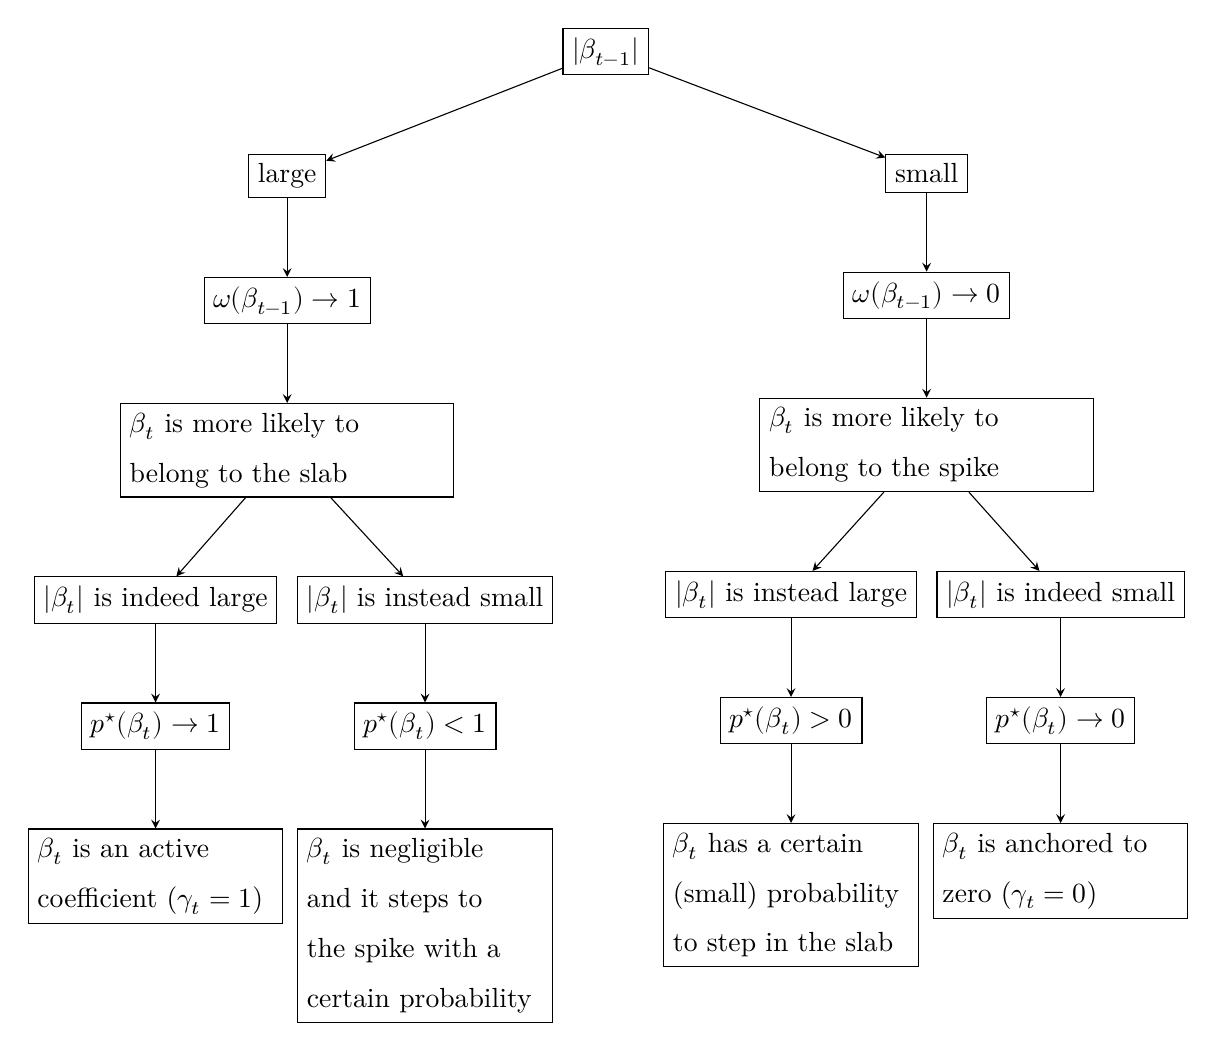
\begin{tikzpicture}[>=stealth]
  \node[draw] (dWdt) {$|\beta_{t-1}|$};
  \node[draw] [below left=1cm and 3cm of dWdt] (large) {large};
  \node[draw] [below right=1cm and 3cm of dWdt] (small) {small};
  \node[draw] [below=of large] (uno) {$\omega(\beta_{t-1})\to1$}; 
  \node[draw] [below=of small] (zero) {$\omega(\beta_{t-1})\to0$};
  \node[draw] [below= of uno,text width=4cm] (slab) {$\beta_{t}$ is more likely to belong to the slab};
  \node[draw] [below= of zero,text width=4cm] (spike) {$\beta_{t}$ is more likely to belong to the spike};
  \node[draw] [below left=1cm and -2cm of slab] (larget) {$|\beta_{t}|$ is indeed large};
  \node[draw] [below right=1cm and -2cm of slab] (smallt) {$|\beta_{t}|$ is instead small};
  \node[draw] [below left=1cm and -2cm of spike] (larget1) {$|\beta_{t}|$ is instead large};
  \node[draw] [below right=1cm and -2cm of spike] (smallt1) {$|\beta_{t}|$ is indeed small};
  \node[draw] [below=of larget] (unot) {$p^{\star}(\beta_{t})\to1$}; 
  \node[draw] [below=of smallt] (zerot) {$p^{\star}(\beta_{t})< 1$};
  \node[draw] [below=of larget1] (unot1) {$p^{\star}(\beta_{t})>0$}; 
  \node[draw] [below=of smallt1] (zerot1) {$p^{\star}(\beta_{t})\to0$};
  \node[draw] [below=of unot,text width=3cm] (cslab) {$\beta_{t}$ is an active coefficient ($\gamma_{t}=1$)}; 
  \node[draw] [below=of zerot,text width=3cm] (cspike) {$\beta_{t}$ is negligible and it steps to the spike with a certain probability}; 
  \node[draw] [below=of unot1,text width=3cm] (cslab1) {$\beta_{t}$ has a certain (small) probability to step in the slab}; 
  \node[draw] [below=of zerot1,text width=3cm] (cspike1) {$\beta_{t}$ is anchored to zero ($\gamma_{t}=0$)}; 
  
  \draw[->] (dWdt) -- (large);
  \draw[->] (dWdt) -- (small);
  \draw[->] (large) -- (uno);
  \draw[->] (small) -- (zero);
  \draw[->] (uno) -- (slab);
  \draw[->] (zero) -- (spike);
  \draw[->] (slab) -- (larget);
  \draw[->] (slab) -- (smallt);
  \draw[->] (spike) -- (larget1);
  \draw[->] (spike) -- (smallt1);
  \draw[->] (larget) -- (unot);
  \draw[->] (smallt) -- (zerot);
  \draw[->] (larget1) -- (unot1);
  \draw[->] (smallt1) -- (zerot1);
  \draw[->] (unot) -- (cslab);
  \draw[->] (zerot) -- (cspike);
   \draw[->] (unot1) -- (cslab1);
  \draw[->] (zerot1) -- (cspike1);
  
\end{tikzpicture}

\section{Dynamic Stochastic Search Variable Selection}\label{Dynamic Stochastic Search Variable Selection}

Efficient posterior simulation of parameters of Time-Varying Parameter
regression models with Dynamic Spike-and-Slab process priors is made
possible thanks to a MCMC algorithm developed by
\protect\hyperlink{ref-rockova_mcalinn_2021}{Rockova and McAlinn}
(\protect\hyperlink{ref-rockova_mcalinn_2021}{2021a}). The latter
consists of a Gibbs sampler which develops in three stages:

\begin{enumerate}
\item Simulate the regression coefficients from $\pi(\boldsymbol{\beta}_{0:T}|\boldsymbol{\gamma}_{0:T},\sigma^{2}_{\epsilon,0:T},y_{1:T})$ using Forward Filter Backward Sampling (FFBS), as illustrated in \emph{Step: 1} of Algorithm \ref{alg:DSSVS-original},
\item Simulate the inclusion indicators from $\pi(\boldsymbol{\gamma}_{0:T}|\boldsymbol{\beta}_{0:T}\sigma^{2}_{\epsilon,0:T},y_{1:T})$ using results of Equations \ref{eq:eq2.8} and \ref{eq:pstar} to compute conditional mixing weights and posterior inclusion probabilities,
\item Simulate the residual variances from $\pi(\sigma^{2}_{\epsilon,0:T}|\boldsymbol{\gamma}_{0:T},\boldsymbol{\beta}_{0:T},y_{1:T})$ using a FFBS strategy as the one illustrated in \emph{Step: 3} of Algorithm \ref{alg:DSSVS-original}.
\end{enumerate}

Since this strategy reminds the SSVS of
\protect\hyperlink{ref-GM_1993}{George and McCulloch}
(\protect\hyperlink{ref-GM_1993}{1993}), then the procedure takes the
label \emph{Dynamic Stochastic Search Variable Selection} (or Dynamic
SSVS). Here we illustrate the original version of the Dynamic SSVS
developed by the authors, which constitute the starting point for the
algorithms developed in the next sections. In particular, we refer to
the Gaussian Spike-and-Slab case introduced previously. Nevertheless,
the procedure described here can be rearranged easily to include a
Laplacian spike instead of a Gaussian one. The Gaussian specification
allow a straightforward and elegant representation of the latent
process, which is the following \begin{equation}
\boldsymbol{\beta}_{t}=\boldsymbol{H}_{t}+\boldsymbol{G}_{t}(\boldsymbol{\beta_{t-1}}-\boldsymbol{H}_{t})+\boldsymbol{\xi}_{t}, \ \ \ \boldsymbol{\xi}_{t}\sim\mathcal{N}(\boldsymbol{0},\Lambda_{t})
\end{equation} where
\(\boldsymbol{H}_{t}=\phi_{0}\boldsymbol{\gamma}_{t}'\),
\(\boldsymbol{G}_{t}=diag\{\gamma_{t,j}\phi_{1}\}_{j=1}^{p}\),
\(\Lambda_{t}=diag\{\gamma_{t,j}\lambda_{1}+(1-\gamma_{t,j})\lambda_{0}\}_{j=1}^{p}\)
and the initial state vector
\(\boldsymbol{\beta}_{0}\sim\mathcal{N}(\boldsymbol{m}_{0},\boldsymbol{C}_{0})\)
with \(\boldsymbol{m}_{0}=\phi_{0}\boldsymbol{\gamma}_{0}\) and
\(\boldsymbol{C}_{0}=diag\{\gamma_{0,j}\lambda_{1}/(1-\phi_{1}^{2})+(1-\gamma_{0,j})\lambda_{0}\}_{j=1}^{p}\).
This model's hyperparameters are
\((\Omega,\lambda_{0},\lambda_{1},\phi_{0},\phi_{1})\), which can be
calibrated or, eventually, treated as random variables by placing a
prior density to them. In this thesis we fix a priori \(\phi_1\) and
\(\phi_0=0\), and we usually assume that \(\phi_0=0\) and \(\phi_1\)
ranges between \(0.98\) and \(0.9\). This of course entails great
simplifications, but seems to work well in all cases we explored. On the
other hand, in its original version the author suggest to treat
\(\phi_1\) as a Beta random variable with support \([0.8,1)\). We see
that the gain due to the latter specification and the drawbacks in terms
of implementation of adding a Metropolis-Hasting step in the Gibbs
sampling scheme compensate each other, that's why we opted for we opted
for a predetermined choice. The hyperparameters \(\lambda_0\) and
\(\lambda_1\) are set a-priori also in the original model
\protect\hyperlink{ref-rockova_mcalinn_2021}{Rockova and McAlinn}
(\protect\hyperlink{ref-rockova_mcalinn_2021}{2021a}).\\
The residual variances are modeled through discount factors. This simple
strategy, developed by \protect\hyperlink{ref-WH_1997}{West and
Harrison} (\protect\hyperlink{ref-WH_1997}{1997}), allows temporal
fluctuations of the model's variance while preserving conjugacy.
Briefly, consider the precision sequence
\(\nu_{t}=\frac{1}{\sigma^{2}_{\epsilon,t}}\) for \(t=1,...,T\). The
latter is assumed to follow a stochastic evolution affected by
independent random shocks \(c_{t}/\delta\), thus
\begin{equation}\label{eq:discountfactor}
\nu_{t}=\frac{c_{t}}{\delta}\nu_{t-1}
\end{equation} where \(\delta\) is the discount factor. It takes values
in \((0,1]\) and it can be regarded as the decay of precision from
period \(t-1\) to \(t\). Therefore, the precision in every period
depends on the previous precision and on the new information that
becomes recursively available. The dynamic of equation
(\ref{eq:discountfactor}) is completed by assuming
\(c_{t}\sim\mathcal{B}(\frac{\delta n_{t-1}}{2},\frac{(1-\delta)n_{t-1}}{2})\)
and \(n_{t}=\delta n_{t-1}+1\). This implies
\(\mathbb E(c_{t}|y_{1:t-1})=\delta\) or, equivalently, that
\(\mathbb E(c_{t}/\delta|y_{1:t-1})=1\). Assigning a Gamma prior on
\(\nu_{0}\sim\mathcal{G}(n_{0},d_{0})\), one can solve the updating
process and solutions in closed form. For \(t>0\), the one-step-ahead
predictive distribution is \begin{equation*}
\nu_{t}|y_{1:t-1},\boldsymbol{\beta}_{1:t-1}\sim\mathcal{G}\bigg(\frac{\delta n_{t-1}}{2},\frac{\delta d_{t-1}}{2}\bigg) 
\end{equation*} which updates into \begin{equation}\label{eq:factmod}
\nu_{t}|y_{1:t},\boldsymbol{\beta}_{1:t}\sim\mathcal{G}\bigg(\frac{n_{t}}{2},\frac{ d_{t}}{2}\bigg) 
\end{equation} with \(n_{t}=\delta n_{t-1}+1\) and
\(d_{t}=\delta d_{t-1}+r^{2}_{t}\), where
\(r_{t}=y_{t}-\boldsymbol{x}_{t}'\boldsymbol{\beta}_{t}\). Posterior
sampling of model's precision can be carried out via a FFBS algorithm
(more details in West and Harrison, 1997). Basically, the filtering
steps follow the updating rule just mentioned, while the backward
sampling consists in drawing from
\(\nu_{T}\sim\mathcal{G}(n_{T}/2,d_{T}/2)\), and then drawing from
\(\eta_{t}\sim\mathcal{G}((1-\delta)n_{t} / 2,d_{t}/2)\) and setting
\(\nu_{t}=\eta_{t}+\delta\nu_{t+1}\) for \(t=T-1,...,0\). This mechanism
is outlined in \emph{Step 3} of Algorithm \ref{alg:DSSVS-original}. Note
that the discount factor strategy for variances estimation can be
reconciled to the standard Bayesian estimation strategy for the unknown
model's variance. Consider for example \begin{align*}
  y_{t}|\boldsymbol{x'}_{t}\boldsymbol{\beta}_{t},\sigma^{2}_{\epsilon} & \overset{ind}{\sim}\mathcal{N}(\boldsymbol{x'}_{t}\boldsymbol{\beta}_{t},\sigma^{2}_{\epsilon}) \\
  \frac{1}{\sigma^{2}_{\epsilon}} \sim & \mathcal{G}\bigg(\frac{n}{2},\frac{d}{2}\bigg)
  \end{align*} Then we have \begin{align*}
\pi(\nu|\boldsymbol{\beta}_{0:T},\boldsymbol{\gamma}_{0:T},y_{1:T})& \propto \pi(\nu,\boldsymbol{\beta}_{0:T},\boldsymbol{\gamma}_{0:T},y_{1:T})\\
&\propto  \pi(y_{1:T}|\nu,\boldsymbol{\beta}_{0:T},\boldsymbol{\gamma}_{0:T})\pi(\boldsymbol{\beta}_{0:T}|\nu,\boldsymbol{\gamma}_{0:T})\pi(\boldsymbol{\gamma}_{0:T}|\nu)\pi(\nu)\\
&\propto  \pi(y_{1:T}|\nu,\boldsymbol{\beta}_{0:T})\pi(\nu)\\
&\propto \prod_{t=1}^{T}\pi(y_{t}|\nu,\boldsymbol{\beta}_{t})\pi(\nu)\\
&\propto \pi(\nu)(\nu)^{T/2}\exp\bigg\{-\frac{\nu}{2}\sum_{t=1}^{T}(y_{t}-\boldsymbol{x}_{t}'\boldsymbol{\beta}_{t})^{2}\bigg\}\\
&\propto \nu^{\frac{n}{2}+T/2+1}\exp\bigg\{-\nu\bigg[\frac{d}{2}+\frac{1}{2}\sum_{t=1}^{T}(y_{t}-\boldsymbol{x}_{t}'\boldsymbol{\beta}_{t})^{2}\bigg]\bigg\}.
\end{align*} Therefore, the full conditional posterior distribution is
\begin{equation*}
\nu|\boldsymbol{\beta}_{0:T},\boldsymbol{\gamma}_{0:T},y_{1:T}\sim\mathcal{G}\bigg(\frac{n+T}{2},\frac{d}{2}+\frac{1}{2}\sum_{t=1}^{T}(y_{t}-\boldsymbol{x}_{t}'\boldsymbol{\beta}_{t})^{2}\bigg)
\end{equation*} which is equivalent to the one obtained using the
discount factor model at time \(T\) for \(\delta=1\). Consequently, no
further challenges are required to step from a stochastic to a constant
volatility model.

The Dynamic SSVS illustrated in this section provides satisfactory
results, however there is room for improvements. Trials performed on
simulated data show indeed that misspecification concerning residual
variances may seriously affect coefficients' estimates. The reason lies
on an artificial bias we detected in the signal-to-noise ratio, which is
decreasing in \(\sigma^{2}_{\epsilon,t}\). We label this phenomenon the
``Spike trap.'' In fact, some irrelevant predictors may activate after
some periods whereas other predictors might leave and re-enter the model
multiple times as time progresses. However, the Dynamic Spike-and-Slab
approach is basically distrustful and it allows steps from the spike to
the slab distribution only if there is enough evidence supporting this
change. This is legitimate and it aims at avoiding abrupt changes from
the spike to the slab densities. However, in certain cases some
coefficients may be forced to the spike even when it is incorrect. On
the other hand, the discounted factor model for the observational
variance is an estimation strategy that heavily relies on cumulated
residuals through \(d_{t}=d_{t-1}+r_{t}^{2}\). However, if the system
fails to recognize some active coefficients in the first iterations of
the Markov Chain, then the residuals
\(r_{t}=y_{t}-\boldsymbol{x}_{t}'\boldsymbol{\beta}_{t}\) become larger
and thus the variances inflate. In other words, the algorithm mistakes
the fluctuations of the observations for variations of the volatility
process rather than changes of the regression coefficients. Eventually,
such a bias can exacerbate in a vicious cycle whereby: the system
erroneously assign a variable to the spike, then the estimated residual
variances inflate and the signal-to-noise ratio decreases. This leads
the algorithm to become even more distrustful of the observations and it
continues to assign those coefficients to the spike.

Nevertheless, this undesirable mechanism can be fixed. In particular,
our proposal is the following. Since the first iterations are the most
critical we recommend to fix the variance at a very low level for the
first loops in such a way that the algorithm strives to understand which
variable can produce the fluctuation observed and then continue with the
MCMC as described. Even though this solution is quite heuristic, we
notice that forcing \(\sigma^{2}_{\epsilon,t}=0.25\) for \(t=1,...,T\)
for just the first 10 loops improves significantly the estimates. In
addition, we developed an alternative Dynamic SSVS which is based on
another strategy for estimating the volatility process and that we found
out to return better performances in terms of accuracy of the estimates
and running time. More details about this method are provided in the
next paragraph.

\begin{algorithm}
\begin{footnotesize}
\caption{Dynamic SSVS by Rockova and McAlinn (2021)} \label{alg:DSSVS-original}
\nl \textbf{Initialize} $\gamma_{j,t}$ and $\sigma^{2}_{\epsilon,t}$ for $0 \leq t \leq T$ and $1 \leq j \leq p$ and set $n_{0}$ and $d_{0}$\;
\begin{center}
\emph{Step 1: Sample Regression Coefficients}\\
\end{center}
\nl \For{$1 \leq t \leq T$}{ 
Compute $\boldsymbol{a}_{t}=\boldsymbol{H}_{t}+\boldsymbol{G}_{t}(\boldsymbol{m}_{t-1}-\boldsymbol{H}_{t})$\;
Compute $\boldsymbol{R}_{t}=\boldsymbol{G}_{t}\boldsymbol{C}_{t-1}\boldsymbol{G}'_{t}+\boldsymbol{\Lambda}_{t}$\;
Compute $f_{t}=\boldsymbol{x}'_{t}\boldsymbol{a}_{t}$ and $e_{t}=y_{t}-f_{t}$\;
Compute $q_{t}=\boldsymbol{x}'_{t}\boldsymbol{R}_{t}\boldsymbol{x}_{t}+\sigma^{2}_{\epsilon,t}$\;
Compute $\boldsymbol{m}_{t}=\boldsymbol{a}_{t}+\boldsymbol{A}_{t}e_{t}$ and $\boldsymbol{C}_{t}=\boldsymbol{R}_{t}-\boldsymbol{A}_{t}\boldsymbol{A}'_{t}q_{t}$ with $\boldsymbol{A}_{t}=\boldsymbol{R}_{t}\boldsymbol{x}_{t}/q_{t}$
}
Draw $\boldsymbol{\beta}_{t}\sim \mathcal{N}(\boldsymbol{m}_{T},\boldsymbol{C}_{t})$\; \For{$t = T-1,...,0$}{  
Compute $\boldsymbol{a}_{T}(t-T)=\boldsymbol{m}_{t}+\boldsymbol{B}_{t}(\boldsymbol{\beta}_{t+1}-\boldsymbol{a}_{t+1})$\;
Compute $\boldsymbol{R}_{t}(t-T)=\boldsymbol{C}_{t}-\boldsymbol{B}_{t}\boldsymbol{R}_{t+1}\boldsymbol{B}'_{t}$ where $\boldsymbol{B}_{t}=\boldsymbol{C}_{t}\boldsymbol{G}'_{t+1}\boldsymbol{R}_{t+1}^{-1}$\;
Draw $\boldsymbol{\beta}_{t}\sim \mathcal{N}(\boldsymbol{a}_{T}(t-T),\boldsymbol{R}_{t}(t-T))$ \;
}
\begin{center}
\emph{Step 2: Sample Indicators}\\
\end{center}
\nl \For{$j=1,...,p$}{
\For{$1 \leq t \leq T$}{
Compute $\omega_{j,t}=\omega(\beta_{j,t-1})$ from \;
Compute $p^{\star}_{t,j}=p^{\star}_{t,j}(\beta_{j,t})$ from \;
Draw $\gamma_{j,t} \sim Bernoulli(p^{\star}_{j,t}(\beta_{j,t}))$\;
}
Compute $p^{\star}_{j,0}=\omega(\beta_{j,0})$\;
Draw $\gamma_{j,0} \sim Bernoulli(p^{\star}_{j,0}(\beta_{j,0}))$\;
}
\begin{center}
\emph{Step 3: Sample Volatility}\\
\end{center}
\nl \For{$t = 1,...,T$}{
Compute $n_{t}=\delta n_{t-1}+1$ and $d_{t}=\delta d_{t-1}+r^{2}_{t}$, where $r_{t}=y_{t}-\boldsymbol{x}_{t}'\boldsymbol{\beta}_{t}$\;
Draw $\nu_{T}\sim\mathcal{G}(n_{T}/2,d_{T}/2)$\;
}
\For{$t=T-1,...,0$}{
Draw $\eta_{t}\sim\mathcal{G}((1-\delta)n_{t} / 2,d_{t}/2)$\;
Set $\nu_{t}=\eta_{t}+\delta\nu_{t+1}$\;
Compute $\sigma^{2}_{\epsilon,t}=\frac{1}{\nu_{t}}$\;
}
\end{footnotesize}
\end{algorithm}

\subsection{Introducing stochastic volatility with Dynamic Spike-and-Slab process priors}\label{A new proposal for the volatility process}

Interestingly, the nature of the MCMC described in Algorithm
\ref{alg:DSSVS-original} allows for a great flexibility in the way the
volatility can be modeled. Indeed, observational variances are sampled
only in \emph{Step 3} and thus our focus will be on the latter, leaving
the first two steps unchanged. Our proposal is to replace the discount
factor model for the variance with a Stochastic Volatility (SV) model.
In the discount factor model, the precision is thought as affected by a
random impulse which is modeled in order to maintain the stability of
the Gamma function. On the other hand a stochastic volatility model
assumes the volatility to be a latent stationary autoregressive process
of unknown parameters \((\alpha_{0},\alpha_{1},\sigma^{2}_{\zeta})\),
with \(|\alpha_{1}|<1\), which are usually considered as random
variables. These class of models has been widely explored and a great
amount of literature has been produced. Given its popularity in the
financial econometrics literature we believe that a stochastic
volatility model is of interest and it is particularly appropriate for
the applications discussed in this thesis. In details, the specification
for the variance here considered is the canonical one reported in the
influential article of \protect\hyperlink{ref-KSC_1998}{Kim, Shephard,
and Chib} (\protect\hyperlink{ref-KSC_1998}{1998}) \begin{align*}
\sigma^{2}_{\epsilon,t}=&\exp^{h_{t}},\\
h_{t}= & \alpha_{0}+\alpha_{1}h_{t-1}+\zeta_{t}, \ \ \ \zeta_{t}\overset{iid}{\sim}\mathcal{N}(0,\sigma^{2}_{\zeta})
\end{align*} Therefore, the new hierarchical setup is \begin{equation}
  \begin{aligned}\label{eq:setup}
  y_{t}|\boldsymbol{x'}_{t}\boldsymbol{\beta}_{t},h_{t} & \overset{ind}{\sim}\mathcal{N}(\boldsymbol{x'}_{t}\boldsymbol{\beta}_{t},\exp{h_{t}}) \\
  \beta_{t,j}|\gamma_{t,j},\beta_{t-1,j} & \overset{ind}{\sim}\mathcal{N}(\gamma_{t,j}\mu_{t,j},\gamma_{t,j}\lambda_{1}+(1-\gamma_{t,j})\lambda_{0})\\
  \gamma_{t,j}|\beta_{t-1,j}\overset{ind}{\sim}& Bernoulli(\omega(\beta_{t-1,j}))\\
  \beta_{0,j}\overset{iid}{\sim}& \mathcal{N}(m_{0},C_{0}) \\
  h_{t}|h_{t-1},\alpha_{0},\alpha_{1},\sigma^{2}_{\zeta}\sim & \mathcal{N}(\alpha_{0}+\alpha_{1}(h_{t-1}-\alpha_0),\sigma^{2}_{\zeta})\\
  h_{0}|\alpha_{0},\alpha_{1},\sigma^{2}_{\zeta}\sim & \mathcal{N}\bigg(\alpha_{0},\frac{\sigma^{2}_{\zeta}}{1-\alpha_{1}}\bigg)
  \end{aligned}
  \end{equation} Note that by taking the residuals, the resulting system
is \begin{equation}
   \begin{aligned}\label{eq:centeredpar}
r_{t} & =e^{\frac{h_{t}}{2}}\epsilon_{t}, \ \ \ \epsilon_{t}\overset{iid}{\sim}\mathcal{N}(0,1) \\
h_{t} & =\alpha_{0}+\alpha_{1}(h_{t-1}-\alpha_0)+\zeta_{t}, \ \ \ \zeta_{t}\overset{iid}{\sim}\mathcal{N}(0,1)
\end{aligned}
\end{equation} which is a standard stochastic volatility model.\\
Over the years, several methods have been developed to estimate this
model. Here, for pragmatism and efficiency, we use the MCMC method
developed of \protect\hyperlink{ref-KASTNER2014408}{Kastner and
Frühwirth-Schnatter} (\protect\hyperlink{ref-KASTNER2014408}{2014}). The
steps described henceforth replace the steps illustrated in
\emph{Step 3} of the original DSS algorithm. The latter considers the
following prior specifications for the unknown stochastic volatility
model's parameters: \begin{align*}
\alpha_{0}\sim & \mathcal{N}(a_{\alpha},A_{\alpha}),\\
(\alpha_{1}+1)/2\sim & \mathcal{B}(a_{0},b_{0}),\\
\pm\sqrt{\sigma^{2}_{\zeta}}\sim & \mathcal{N}(0,A_{\sigma_{\zeta}})
\end{align*} A recommended choice for the hyperparameters in our problem
is too set them in such a way that the stochastic volatility process
would not show abrupt changes. For example we can guess:
\(\alpha_{0}\sim \mathcal{N}(-2,10)\),
\((\alpha_{1}+1)/2\sim \mathcal{B}(20,1.5)\) such that
\(\mathbb E(\alpha_1)=0.86\) and \(\mathbb V(\alpha_1)=0.11\), and
\(A_{\sigma_{\zeta}}=1\) or even less. Draws from the posterior
distributions are obtained using a fast simulation procedure provided by
the \texttt{stochvol} package (\protect\hyperlink{ref-SV_2016}{Kastner
2016}). The rapidity of the algorithm is guaranteed by sampling
volatilities jointly ``all without a loop'' (AWOL), a techinque which is
exhaustively described in
\protect\hyperlink{ref-MCCAUSLAND2011199}{McCausland, Miller, and
Pelletier} (\protect\hyperlink{ref-MCCAUSLAND2011199}{2011}), and by
using the ``ancillarity-sufficiency interweaving strategy'' (ASIS)
developed by \protect\hyperlink{ref-YM_2011}{Yu and Meng}
(\protect\hyperlink{ref-YM_2011}{2011}). In a nutshell, the ASIS
strategy is based on a simple intuition, i.e.~every SV models can be
written in a \emph{centered parametrization (C)} form, which is the one
of equation (\ref{eq:centeredpar}), or alternatively in a
\emph{non-centered parametrization (NC)} form, that is \begin{equation}
   \begin{aligned}\label{eq:centeredparr}
r_{t} & \sim \mathcal{N}(0,e^{\mu}e^{\sigma \tilde{h}_{t}}),\\
\tilde{h}_{t} & =\alpha_{1}\tilde{h}_{t-1}+\sigma_{\zeta}\zeta_{t}, \ \ \ \zeta_{t}\overset{iid}{\sim}\mathcal{N}(0,1)
\end{aligned}
\end{equation} where
\(\tilde{h}_{t}=(h_{t}-\alpha_{0})/\sigma_{\zeta}\). It is immediate to
notice that \(h_{1:T}\) is a sufficient statistic for \(\alpha_0\) and
\(\alpha_1\) in C, while \(\tilde{h}_{1:T}\) in NC is ancillary for the
same parameters. Therefore, sampling can be improved by interwaving
between the two parametrizations. \protect\hyperlink{ref-YM_2011}{Yu and
Meng} (\protect\hyperlink{ref-YM_2011}{2011}) link this results to the
Basu's theorem, which demonstrates independence among complete
sufficient and ancillary statistics. Operationally, the strategy
consists in sampling \(\alpha_{0},\alpha_{1},\sigma^{2}_{\zeta}\) twice:
once in C and once in NC. Therefore, let
\(\tilde{r}_{t}=\log{r_{t}}^{2}\) and let's approximate
\(\tilde{\epsilon}=\log\epsilon^{2}_{t}\) with a mixture of normal
distributions such that
\(\log\epsilon^{2}_{t}|i_{t}\overset{iid}{\sim}\mathcal{N}(m_{i_t},s_{i_t}^{2})\),
where \(i_{t} \in \{1,...,10\}\) is a mixture component indicator at
period \(t\), then consider the following linear and conditionally
Gaussian approximation of a SV model: \[
\tilde{r}_{t} = m_{i_t}+h_{t}+\tilde{\epsilon}_t, \quad \tilde{\epsilon}_{t}\overset{iid}{\sim}\mathcal{N}(0,s_{i_t}^2)
\] A MCMC algorithm to simulate from \begin{align*}
\tilde{r}_{t} & =  m_{i_t}+h_{t}+\tilde{\epsilon}_t, \quad \tilde{\epsilon}_{t}\overset{iid}{\sim}\mathcal{N}(0,s_{i_t}^2),\\
h_{t} & = \alpha_{0}+\alpha_{1}(h_{t-1}-\alpha_0)+\zeta_{t}, \ \ \ \zeta_{t}\overset{iid}{\sim}\mathcal{N}(0,1),
\end{align*} can be performed in this way:

\begin{enumerate}
\item Sample $h_{1:T}$ AWOL from $h_{1:T}\mid r_t,i_t,\alpha_0,\alpha_1,\sigma^2_\zeta \sim \mathcal{N}(\Xi^{-1} \boldsymbol{c},\Xi^{-1})$ in C, where 
\[
\Xi = \begin{pmatrix}
  \frac{1}{s^{2}_{i_1}}+\frac{1}{\sigma^2_\zeta} & \frac{-\alpha_1}{\sigma^{2}_{\zeta}} & 0 & ... & 0 \\
  \frac{-\alpha_1}{\sigma^{2}_{\zeta}} & \frac{1}{s^{2}_{i_1}}+\frac{1+\alpha_1^2}{\sigma^2_\zeta} & \frac{-\alpha_1}{\sigma^{2}_{\zeta}} & \ddots & \vdots \\
  0  &  \frac{-\alpha_1}{\sigma^{2}_{\zeta}} & \ddots & \ddots & 0\\
  \vdots & \ddots & \ddots & \frac{1}{s^{2}_{i_{T-1}}}+\frac{1+\alpha_1}{\sigma^2_\zeta} & \frac{-\alpha_1}{\sigma^{2}_{\zeta}}\\
  0 & \cdots & 0 & \frac{-\alpha_1}{\sigma^{2}_{\zeta}} & \frac{1}{s^{2}_{i_{T}}}+\frac{1}{\sigma^2_\zeta}
  \end{pmatrix}
\]
and 
\[
\boldsymbol{c}= \begin{pmatrix} 
\frac{1}{s^{2}_{i_1}}(\tilde{r}_{1}-m_{i_1})+\frac{\alpha_{0}(1-\alpha_1)}{\sigma^{2}_{\zeta}}\\
\frac{1}{s^{2}_{i_2}}(\tilde{r}_{2}-m_{i_2})+\frac{\alpha_{0}(1-\alpha_1)^2}{\sigma^{2}_{\zeta}}\\
\vdots \\
\frac{1}{s^{2}_{i_{T-1}}}(\tilde{r}_{T-1}-m_{i_{T-1}})+\frac{\alpha_{0}(1-\alpha_1)^2}{\sigma^{2}_{\zeta}}\\
\frac{1}{s^{2}_{i_T}}(\tilde{r}_{2}-m_{i_T})+\frac{\alpha_{0}(1-\alpha_1)}{\sigma^{2}_{\zeta}}
\end{pmatrix}
\]
and sample $h_0$ from $\pi(h_{0}\mid h_{1},\alpha_1,\sigma^{2}_{\zeta})$.
\item Sample $\alpha_0,\alpha_1,\sigma^2_\zeta$. In C, it is possible to draw the parameters jointly from $\pi(\alpha_0,\alpha_1,\sigma^2_\zeta\mid h_{1:T})$ using a single Metropolis-Hastings step. Let $\rho=(1-\alpha_1)\alpha_0$ and $\boldsymbol{\psi}=(\alpha_0,\alpha_1,\sigma^2_\zeta)$, the proposal density can be wisely chose as
\[
\pi_{aux}(\boldsymbol{\psi}^{(\text{new})}\mid h_{0:T})=\pi_{aux}(\rho^{(\text{new})},\alpha_1^{(\text{new})}\mid h_{0:T},{\sigma^{2}_{\zeta}}^{(\text{new})})\pi_{aux}({\sigma^{2}_{\zeta}}^{(\text{new})}\mid h_{0:T})
\]
and $\pi_{aux}(\sigma^2_{\zeta})\propto \sigma^{-1}_{\zeta}$ and $\pi_{aux}(\rho,\alpha_1\mid \sigma^{2}_{\zeta})\sim \mathcal{N}(\boldsymbol{0},\sigma^{2}\boldsymbol{B}_{0})$ with $\boldsymbol{B}_{0}=diag(B_{0}^{11},B_{0}^{22})$. Therefore, the posteriors are 
\[
\rho,\alpha_1\mid h_{0:T},\sigma^{2}_{\zeta}\sim\mathcal{N}(\boldsymbol{b}_{T},\sigma^{2}_{\zeta}\boldsymbol{B}_{T})
\]
with $\boldsymbol{B}_{T}=(\boldsymbol{H}'\boldsymbol{H}+\boldsymbol{B}_{0}^{-1})^{-1}$ and $\boldsymbol{b}_{T}=\boldsymbol{B}_{T}\boldsymbol{H}'h_{1:T}'$, where $\boldsymbol{H}$ is a $T \times 2$ matrix $\boldsymbol{H}=(\boldsymbol{1}_{T}',h_{0:T-1}')$, and 
\[
\sigma^{2}_{\zeta}\mid h_{0:T}\sim \mathcal{IG}(c_{T},C_{T})
\]
with $c_{T}=(T-1)/2$ and $C_T=\frac{1}{2}(\sum_{t=1}^{T}h_{t}^{2}-\boldsymbol{b}_{T}'\boldsymbol{H}'h_{1:T}')$. The acceptance probability is $\min(1,R)$ where
\[
R = \frac{\pi(h_0\mid \boldsymbol{\psi}^{\text{(new)}})\pi(\rho^{\text{(new)}}\mid \alpha_1^{\text{(new)}})\pi({\sigma^{2}_{\zeta}}^{\text{(new)}})}{\pi(h_0\mid \boldsymbol{\psi}^{\text{(old)}})\pi(\rho^{\text{(old)}}\mid \alpha_1^{\text{(old)}})\pi({\sigma^{2}_{\zeta}}^{\text{(old)}})} \times \frac{\pi_{aux}(\alpha_1^{\text{(old)}},\rho^{\text{(old)}}\mid {\sigma^{2}_{\zeta}}^{\text{(old)}})}{\pi_{aux}(\alpha_1^{\text{(new)}},\rho^{\text{(new)}}\mid {\sigma^{2}_{\zeta}}^{\text{(new)}})}.
\]

Alternatively, one can use a 2-block sampler that draw from $\pi(\sigma^2_\zeta\mid h_{1:T},\alpha_0,\alpha_1)$ and  $\pi(\alpha_0,\alpha_1\mid h_{1:T},\sigma^2_\zeta)$, or sample them individually from their full conditional distributions. 
\item Shift to NC using the transformation $\tilde{h}_{t}=(h_{t}-\alpha_0)/\alpha_1$ for $t=1,...,T$.
\item Draw again $\alpha_0,\alpha_1,\sigma^2_\zeta$. In NC, use Metropolis-Hastings for sampling from $\pi(\alpha_1\mid\tilde{h}_{1:T})$ and then sample $\alpha_0$ and $\sigma^2_\zeta$ jointly from $\pi(\alpha_0,\sigma^2_\zeta\mid r_{1:T},\tilde{h}_{1:T},i_{1:T})$. In details, to sample $\alpha_1$, which is the only parameter in the state equation, one can use an improper auxiliary prior $\pi_{aux}(\alpha_1)\propto c$, with posterior
\[
\alpha_1\mid\tilde{h}_{0:T}\sim\mathcal{N}\bigg(\frac{\sum_{t=0}^{T-1}\tilde{h}_{t}\tilde{h}_{t+1}}{\sum_{t=0}^{T-1}\tilde{h}_{t}^{2}},\frac{1}{\sum_{t=0}^{T-1}\tilde{h}_{t}^{2}}\bigg)
\]
and acceptance probability $\min(1,R)$, where 
\[
R = \pi(\tilde{h}_{0}\mid\alpha_{1}^{(\text{new})})\pi(\alpha_1^{(\text{new})})/\pi(\tilde{h}_{0}\mid \alpha_1^{(\text{old})})\pi(\alpha_1^{\text{(old)}}).
\]
Then, samples of $\alpha_0$ and $\sigma^2_\zeta$ are obtained starting from the regression model
\[
\hat{\boldsymbol{r}}=\boldsymbol{H}\begin{pmatrix}\alpha_0 \\ \sigma^2_\zeta \end{pmatrix} + \boldsymbol{\epsilon}, 
\]
where $\boldsymbol{\epsilon}\sim \mathcal{N}(\boldsymbol{0},\boldsymbol{I}_{T})$, 
\[
\hat{\boldsymbol{r}} = \begin{pmatrix} 
(\tilde{r}_{1}-m_{i_1})/s_{i_1} \\ 
\vdots \\
(\tilde{r}_{T}-m_{i_T})/s_{i_T}
\end{pmatrix}
\]
and 
\[
\boldsymbol{H} = \begin{pmatrix} 
\tilde{h}_{1}/s_{i_1} &  1/s_{i_1} \\ 
\vdots \\
\tilde{h}_{T}/s_{i_T} &  1/s_{i_T}
\end{pmatrix}.
\]

The posterior distribution $\pi(\alpha_0,\sigma^{2}_{\zeta}\mid r_{1:T},\tilde{h}_{0:T},i_{1:T})$ is thus $\mathcal{N}(\boldsymbol{b}_{T},\boldsymbol{B}_{T})$ with $\boldsymbol{B}_{T}=(\boldsymbol{H}'\boldsymbol{H}+\boldsymbol{B}_{0}^{-1})^{-1}$ and $\boldsymbol{b}_{T}=\boldsymbol{B}_{T}(\boldsymbol{B}^{-1}_{0}\boldsymbol{\beta}_{0}+\boldsymbol{H}'\boldsymbol{r})$, where $\boldsymbol{b}_{0}=(b_{\alpha_0},0)'$ and $\boldsymbol{B}_{0}=diag(B_{\alpha_0},B_{\sigma_\zeta})$.\
Alternatively, one can sample $(\alpha_0,\sigma^2_\zeta)$ individually form $\pi(\alpha_0\mid r_{1:T},\tilde{h}_{1:T},i_{1:T},\sigma^2_\zeta)$ and $\pi(\sigma^2_\zeta\mid r_{1:T},\tilde{h}_{1:T},i_{1:T},\alpha_0)$.
\item Return to C by computing $h_{t}=\alpha_{0}+\sigma_\zeta \tilde{h}_t$ for $t=1,...,T$
\item Draw $i_t$ from $\pi(i_{t}\mid r_{1:T},h_{1:T})$ in C. Given that $\tilde{r}_{t}-h_{t}=\epsilon^{*}_{t}$, with $\epsilon^{*}_{t}\sim\mathcal{N}(m_{i_t},s^{2}_{i_t})$, then the posterior probability of $i_{1:T}\mid r_{1:T},h_{0:T}$ is 
\[
\mathbb{P}(i_{t}=k|r_{1:T},h_{0:T}) \propto \mathbb{P}(i_t=k)\frac{1}{s_k}\exp\bigg\{-\frac{(\epsilon^{*}-m_{k})^2}{2s_{k}^2}\bigg\}
\]
for $k \in \{1,...,10\}$ and $t \in \{1,...,T\}$, where $\mathbb{P}(i_t=k)$ are the mixture weights of the $k$th component.
\end{enumerate}

So far, we described the procedure starting in C, however it is also
possible to start in NC, then move to C and finally return back to NC.
For more details on the AWOL-ASIS strategy, the reference is
\protect\hyperlink{ref-KASTNER2014408}{Kastner and Frühwirth-Schnatter}
(\protect\hyperlink{ref-KASTNER2014408}{2014}).

\subsection{Speeding up MCMC with a precision sampler}\label{Sparse Matrix}

In order to speed up the Dynamic SSVS, we also propose an alternative
estimation and simulation technique for the regression coefficients. As
already mentioned in Chapter 1, the computational complexity of the
Kalman filter is linear in the length of the data and quadratic in the
dimension of the state vector. This turns out to be a downside in the
context we are considering which is characterized by several latent
processes, as many as the predictors inside the model. The AWOL method
to sample from the posterior distributions of the SV model allows to
slightly reduce the running time, however the major computational effort
comes from the FFBS step for the regression coefficients. Therefore, we
decide to try a different approach for sampling the
\(\boldsymbol{\beta}_{0:T}\), namely the precision sampler of
\protect\hyperlink{ref-chan_jeliazkov_2009}{Chan and Jeliazkov}
(\protect\hyperlink{ref-chan_jeliazkov_2009}{2009}). The latter is based
on sparse matrix routines and it has been developed for multivariate
time series. We describe it using the notation of the authors which will
be resumed in Chapter 4. In particular we follow
\protect\hyperlink{ref-Chan_2018}{Chan and Eisenstat}
(\protect\hyperlink{ref-Chan_2018}{2018}). In fact, the Gibbs sampler
proposed here extends the original precision sampler, in taking into
account the dynamic shrinkage expressed through the DSS process prior.
Let \(\boldsymbol{y} = (\boldsymbol{y}_{1}',...,\boldsymbol{y}_{T}')'\),
where \(\boldsymbol{y}_{t}=(y_{t,1},...,y_{t,n})'\), and
\(\boldsymbol{\theta} = (\boldsymbol{\theta}_{1}',...,\boldsymbol{\theta}_{T}')'\),
where in the TVP Regression model
\(\boldsymbol{\theta}=\boldsymbol{\beta}\) and
\(\boldsymbol{\theta}_{t}=(\theta_{t,1},...,\theta_{t,p})'\) The Gibbs
sampling follows the scheme \ref{alg:sparsemat}. \begingroup
\LinesNumbered

\begin{algorithm}[t]
\caption{Dynamic Shrinkage in the Precision Sampler of Chan and Jeliazkov (2009) } \label{alg:sparsemat}
 Sample from $\pi(\boldsymbol{\theta}|\boldsymbol{y},\boldsymbol{h},\boldsymbol{\gamma},\boldsymbol{\theta}_{0})$ \;
 Sample from $\pi(\boldsymbol{\theta}_{0}|\boldsymbol{y},\boldsymbol{h},\boldsymbol{\gamma},\boldsymbol{\theta})$ \;
 Sample individually and independently from $\pi(\gamma_{j,t}|\boldsymbol{y},\boldsymbol{h},\boldsymbol{\theta},\boldsymbol{\theta}_{0},\gamma_{-j,t})$ \;
 Compute $\boldsymbol{\Lambda}=diag\{\boldsymbol{\gamma}\lambda_{1}+(\boldsymbol{1}-\boldsymbol{\gamma})\lambda_{0}\}$\;
 Compute $\boldsymbol{D}$ as in equation (\ref{eq:D})\;
 Sample from $\pi(\boldsymbol{h}|\boldsymbol{y},\boldsymbol{\theta},\boldsymbol{\gamma},\boldsymbol{\theta}_{0},\boldsymbol{\Psi})$ \;
\end{algorithm}
\endgroup

Note: in Algorithm \ref{alg:sparsemat}, the sampling of
\(\boldsymbol{\Psi}=\{\alpha_{0,i},\alpha_{1,i},\sigma^{2}_{\zeta,i}\}_{i=1}^{n}\)
is implicit, but it consists of the same steps described in Section
\ref{A new proposal for the volatility process}. Because of the large
number of parameters to be estimated in multivariate time series, it
seems a reasonable simplifying assumption to use a random walk for the
volatility,
i.e.~\(\boldsymbol{h}_{t}=\boldsymbol{h}_{t-1}+\boldsymbol{\zeta}_{t}\)
with
\(\boldsymbol{\zeta}_{t}\sim\mathcal{N}(\boldsymbol{0},\Sigma_{\zeta})\)
and \(\Sigma_{\zeta}=diag\{\sigma^{2}_{i}\}_{i=1}^{n}\). Let's focus on
each step.

\begin{itemize}
\item Step 1; Let us recall the state space representation of a TVP-VAR model 
\[\underset{(T \times n)\times1}{\boldsymbol{y}}=\underset{(T\times n)\times p}{\boldsymbol{X}}\ \ \underset{p\times 1}{\boldsymbol{\theta}} + \underset{(T \times n)\times1}{\boldsymbol{\epsilon}}, \ \ \ \boldsymbol{\epsilon} \sim \mathcal{N}\bigg(\underset{(T \times n)\times1}{\boldsymbol{0}},\underset{(T \times n)\times (T\times n)}{\boldsymbol{\Sigma}}\bigg)\]
where $\boldsymbol{\epsilon} = (\boldsymbol{\epsilon}_{1}',...,\boldsymbol{\epsilon}_{T}')'$, $\boldsymbol{\Sigma} = diag(\Sigma_{\epsilon,1},...,\Sigma_{\epsilon,T})$ and $\boldsymbol{X} = diag(\boldsymbol{X}_{1},...,\boldsymbol{X}_{T})$, and the latent process of the stochastic coefficients evolves as 
\[\boldsymbol{\theta}_{t}=\boldsymbol{G}_{t}\boldsymbol{\theta}_{t-1}+\boldsymbol{\eta}_{t}, \ \ \ \boldsymbol{\eta}_{t} \sim \mathcal{N}(\boldsymbol{0},\Lambda_{t})\]
where in the DSS scheme $\boldsymbol{G}_{t}=diag\{\gamma_{j,t}\phi_{1}\}_{j=1}^{p}$ and $\Lambda_{t}=diag\{\gamma_{j,t}\lambda_{1}+(1-\gamma_{j,t})\lambda_{0}\}_{j=1}^{p}$. \
Define the matrix 
\begin{equation} \label{eq:D}
\boldsymbol{D} = \begin{pmatrix}
\boldsymbol{I}_{k} & 0 & ... & 0\\
-\boldsymbol{G}_{1} & \boldsymbol{I}_{k} & ... & 0\\
... & ... & ... & 0 \\
0 & ... & -\boldsymbol{G}_{T} & \boldsymbol{I}_{k}
\end{pmatrix}
\end{equation}
Therefore we can write
\[  \boldsymbol{D}\boldsymbol{\theta} = \boldsymbol{\tilde{\alpha}}_{0}+\boldsymbol{\xi}, \ \ \ \boldsymbol{\xi} \sim \mathcal{N}(\boldsymbol{0},\boldsymbol{S_\theta}) \]
where $\boldsymbol{\tilde{\alpha}}_{0}=(\boldsymbol{\theta}'_{0},\boldsymbol{0},...\boldsymbol{0})'$ and $\boldsymbol{S_\theta}=diag(\Lambda_{1},...,\Lambda_{T})$.
Equivalently we write
\[\boldsymbol{\theta} | \boldsymbol{\theta}_{0},\boldsymbol{\gamma} \sim \mathcal{N}(\boldsymbol{D}^{-1}\boldsymbol{\tilde{\alpha}}_{0},(\boldsymbol{D}'\boldsymbol{S_\theta}^{-1}\boldsymbol{D})^{-1})\]
and we label $\boldsymbol{\alpha}_{0}=\boldsymbol{D}^{-1}\boldsymbol{\tilde{\alpha}}_{0}$.
Thanks to Corollary 8.1 of Theorem 8.1 of Kroese and Chan (2014), that we mentioned in Section \ref{Bayesian Inference in Linear Regression}, we can sample from 
\[\boldsymbol{\theta} | \boldsymbol{y},\boldsymbol{h},\boldsymbol{\gamma},\boldsymbol{\theta}_{0},\boldsymbol{h}_{0} \sim \mathcal{N}(\hat{\boldsymbol{\theta}},\boldsymbol{K}^{-1}_{\boldsymbol{\theta}})\]
where $\hat{\boldsymbol{\theta}}=\boldsymbol{K}^{-1}_{\boldsymbol{\theta}}\boldsymbol{d}_{\boldsymbol{\theta}}$, $\boldsymbol{K_\theta}=\boldsymbol{D}'\boldsymbol{S_\theta}^{-1}\boldsymbol{D}+\boldsymbol{X}'\boldsymbol{\Sigma_\epsilon}^{-1}\boldsymbol{X}$ and $\boldsymbol{d_\theta}=\boldsymbol{D}'\boldsymbol{S_\theta}^{-1}\boldsymbol{D}\boldsymbol{\alpha}_{0}+\boldsymbol{X}'\boldsymbol{\Sigma_{\epsilon}}^{-1}\boldsymbol{y}$.
\item Step 2; Sample $\boldsymbol{\theta}_{0}$ from the full conditional distribution 
\[
(\boldsymbol{\theta}_{0}|\boldsymbol{y},\boldsymbol{\theta},\boldsymbol{h},\boldsymbol{\Lambda}_{0})\sim\mathcal{N}(\hat{\boldsymbol{\theta}_{0}},\boldsymbol{K_{\theta_{0}}}^{-1})
\]
where $\boldsymbol{K_{\theta_{0}}}=\boldsymbol{C}_{0}^{-1}+\Lambda^{-1}_{0}$ and $\hat{\boldsymbol{\theta}_{0}}=\boldsymbol{K_{\theta_{0}}}^{-1}(\boldsymbol{C}_{0}^{-1}\boldsymbol{m}_{0}+\Lambda_{0}^{-1}\boldsymbol{\theta}_{1})$, with $\boldsymbol{m}_{0}$ and $C_{0}$ respectively the prior mean and the prior variance of the state vector.
\item Step 3; Sample individually and independently the indicators $\gamma_{j,t}$ from their full conditional distribution as in Step 2 of Algorithm \ref{alg:DSSVS-original}.
\item Step 6; Compute $\boldsymbol{r}=\boldsymbol{y}-\boldsymbol{X}\boldsymbol{\theta}$ and use the residuals $\boldsymbol{r}_{i}=(r_{1,i},...,r_{T,i})'$ (for $i=1,...,n$) to perform the AWOL-ASIS strategy of Kastner (2016).
\end{itemize}

In alternative to \protect\hyperlink{ref-KASTNER2014408}{Kastner and
Frühwirth-Schnatter} (\protect\hyperlink{ref-KASTNER2014408}{2014}), the
authors of the precision sampler use the computational strategy of
\protect\hyperlink{ref-KSC_1998}{Kim, Shephard, and Chib}
(\protect\hyperlink{ref-KSC_1998}{1998}). In this case it is also
necessary to sample \(\boldsymbol{h}_{0}\) from the full conditional
distribution \[
(\boldsymbol{h}_{0}|\boldsymbol{y},\boldsymbol{h},\boldsymbol{\theta},\boldsymbol{\Lambda}_{0},\Sigma_{\zeta})\sim\mathcal{N}(\hat{\boldsymbol{h}_{0}},\boldsymbol{K_{h_{0}}}^{-1})
\] where
\(\boldsymbol{K_{h_{0}}}=\boldsymbol{V}^{-1}_{h}+\Sigma_{\zeta}^{-1}\)
and
\(\hat{\boldsymbol{h}_{0}}=\boldsymbol{K_{h_{0}}}^{-1}(\boldsymbol{V}^{-1}_{h}\boldsymbol{a}_h+\Sigma_{\zeta}^{-1}\boldsymbol{h}_{1})\),
and \(\boldsymbol{a}_{h}\) and \(\boldsymbol{V}_{h}\) are the prior mean
and variance of the initial volatility state.

\section{Dynamic Expectation-Maximization Variable Selection}\label{Dynamic EMVS}

A valuable alternative to simulation algorithms come from
\protect\hyperlink{ref-rockova_mcalinn_2021}{Rockova and McAlinn}
(\protect\hyperlink{ref-rockova_mcalinn_2021}{2021a}). They propose an
innovative optimization approach to variable selection based on an
Expectation-Maximization (EM) algorithm which is labelled by the authors
Dynamic Expectation-Maximization Variable Selection or, more briefly,
Dynamic EMVS. This method aims at providing the Maximum A Posteriori
(MAP) estimate
\(\boldsymbol{\hat{\beta}}_{1:T}=\arg\max\pi(\boldsymbol{\beta}_{1:T}|y_{1:T})\)
by reducing this challenging maximization problem into a sequence of
simpler maximization steps. Each iteration is indeed decomposed into two
stages. In the first step, known as E-Step, the conditional expectations
of the unknown model's parameters is computed given the observations and
the other parameters of interest. The second step, or M-step, consists
in maximizing the joint conditional expectation of the model's
parameters given the observations, where the other unknown model's
parameters are treated as missing values and are replaced by their
conditional expectation. In our specific case, these two passages
become:

\begin{center}
\begin{itemize}
\item \emph{E-step:} Compute $\mathbb E(\boldsymbol{\gamma}_{0:T},\sigma^2_{\epsilon,1:T}\mid \boldsymbol{\beta}^{(m)}_{0:T},y_{1:T})$, where $\boldsymbol{\beta}_{0:T}^{(m)}$ indicates the regression coefficients sequence at the $m^{th}$ iteration.
\item \emph{M-step:} Maximize $\mathbb E_{\boldsymbol{\gamma}_{0:T},\sigma^2_{\epsilon,1:T} \mid \cdot }\log\pi(\boldsymbol{\beta}_{0:T},\boldsymbol{\gamma}_{0:T},\sigma^{2}_{\epsilon,1:T}\mid y_{1:T})$ with respect to $\boldsymbol{\beta}_{0:T}$.
\end{itemize}
\end{center}

In details, since \(\boldsymbol{\gamma}_{0:T}\) and
\(\sigma^2_{\epsilon,1:T}\) are conditionally independent, we compute
\(\mathbb E(\boldsymbol{\gamma}_{0:T}\mid\boldsymbol{\beta}_{0:T},y_{1:T})\)
and
\(\mathbb E(\sigma^2_{\epsilon,1:T}\mid\boldsymbol{\beta}_{0:T},y_{1:T})\).
The first boils down in computing
\(p^{\star}_{t,j} = \mathbb{P}(\gamma_{t,j}=1 \mid \beta_{t,j}^{(m)},\beta_{t-1,j}^{(m)},\Omega)\)
for \(t=0,...,T\) and \(j=1,...,p\). The latter depends on the
specification of the variances used in the model. For example,
considering the discount factor model for the volatility of equation
(\ref{eq:discountfactor}), it can be shown
(\protect\hyperlink{ref-WH_1997}{West and Harrison 1997}) that \[
\mathbb E(\nu_{t}\mid\boldsymbol{\beta}^{(m)}_{0:T},y_{1:T})=(1-\delta)n_{t}/d_{t}+\delta\mathbb E(\nu_{t+1}\mid\boldsymbol{\beta}^{(m)}_{0:T},y_{1:T})
\] for \(1\leq t <T\), and
\(\mathbb E(\nu_{t}\mid\boldsymbol{\beta}^{(m)}_{0:T},y_{1:T})=n_{T}/d_{T}\).
On the other hand, the non-linearity introduced by specifying the
volatility as a log-Normal AR(1) process does not allow to obtain first
moments in closed form. For this reason, we developed a novel approach
characterized by particle filtering and smoothing in the E-step. At the
cost of a slight increase in the running time, the new algorithm
provides with better volatility estimates. More details of this methods
are provided in the next section.\\
The M-step requires some considerations too. Here, we describe the
Gaussian Spike-and-Slab case; for the Laplace case we refer to
\protect\hyperlink{ref-rockova_mcalinn_2021}{Rockova and McAlinn}
(\protect\hyperlink{ref-rockova_mcalinn_2021}{2021a}). The initial state
vector, \(\boldsymbol{\beta}_{0}\), is estimated with the whole state
sequence \(\boldsymbol{\beta}_{1:T}\) and, according to the DSS
specification, it is assumed to have a stationary distribution
\begin{equation}
\pi(\boldsymbol{\beta}_{0}|\boldsymbol{\gamma}_{0})=\prod_{j=1}^{p}[\gamma_{0,j}\psi_{1}^{ST}(\beta_{0,j}|\lambda_{1},\phi_{0},\phi_{1})+(1-\gamma_{0,j})\psi_{0}(\beta_{0,j}|\lambda_{0})]
\end{equation} where \(\gamma_{0,j}| \Omega\sim Bernoulli(\Omega)\) for
\(j=1,...,p\). Notice that the Markov structure of the models parameters
and their independence allow the following factorization
\begin{equation}
\pi(\boldsymbol{\beta}_{0:T},\boldsymbol{\gamma}_{0:T},\sigma^2_{\epsilon,1:T})=\pi(\boldsymbol{\beta}_{0}|\boldsymbol{\gamma}_{0})\pi(\boldsymbol{\gamma}_{0})\prod_{t=1}^{T}\bigg[\pi(\sigma^2_{\epsilon,t}|\sigma^2_{\epsilon,t-1})\prod_{j=1}^{p}\pi(\beta_{t,j}|\gamma_{t,j},\beta_{t-1,j})\pi(\gamma_{t,j}|\beta_{t-1,j})\bigg]
\end{equation} Then we can write \begin{equation}
   \begin{aligned}\label{eq:objfun}
 & \log \pi(\boldsymbol{\beta}_{0:T},\boldsymbol{\gamma}_{0:T},\sigma^2_{\epsilon,1:T}|y_{1:T})
 \\  & = C+\sum_{t=1}^{T}\sum_{j=1}^{p}[\gamma_{t,j}\log \theta_{t,j}+(1-\gamma_{t,j})\log(1-\theta_{t,j})] 
\\ & - \sum_{t=1}^{T}\bigg\{\frac{(y_{t}-\boldsymbol{x}_{t}'\boldsymbol{\beta}_{t})^{2}}{2\sigma^{2}_{\epsilon,t}}+\sum_{j=1}^{p}\bigg[\gamma_{t,j}\frac{(\beta_{t,j}-\phi_{1}\beta_{t-1,j})^{2}}{2\lambda_{1}}+(1-\gamma_{t,j})\frac{\beta_{t,j}^{2}}{2\lambda_{0}}\bigg]+\log\pi(\sigma^2_{\epsilon,t}|\sigma^2_{\epsilon,t-1})\bigg\} 
\\ & - \sum_{j=1}^{p}\bigg\{\gamma_{0,j}\frac{\beta_{0,j}^{2}(1-\phi_{1}^{2})}{2\lambda_{1}}+(1-\gamma_{0,j})\frac{\beta_{0,j}^{2}}{2\lambda_{0}}-\gamma_{0,j}\log\Omega-(1-\gamma_{0,j})\log(1-\Omega)\bigg\}
\end{aligned}
\end{equation} where \(C\) incorporates all the constant components. Let
\(\nu_t = \frac{1}{\sigma^{2}_{\epsilon,t}}\), the objective function we
want maximize in the M-step is
\(\mathbb E_{\boldsymbol{\gamma}_{0:T},\nu_{1:T} \mid \cdot }\log\pi(\boldsymbol{\beta}_{0:T},\boldsymbol{\gamma}_{0:T},\nu_{1:T}\mid y_{1:T})=Q(\boldsymbol{\Xi}\mid y_{1:T})\).
Therefore, we replace \((\boldsymbol{\gamma}_{0:T},\nu_{1:T})\) in
equation (\ref{eq:objfun}) with their conditional expectations
\((\boldsymbol{p}^{\star}_{0:T},\nu^{\star}_{1:T})\) computed in the
E-step. Then, we find the maximum of \(Q(\boldsymbol{\Xi}\mid y_{1:T})\)
with respect to \(\boldsymbol{\beta}_{0:T}\). Below we report the first
order conditions: \begin{align*}
\frac{\partial Q(\boldsymbol{\Xi} \mid y_{1:t})}{\partial \boldsymbol{\beta}_{t}} = 0 & \iff \boldsymbol{\beta}_{t} = \boldsymbol{D}_{t}^{-1}\bigg\{\nu_{t}^{\star}y_{t}\boldsymbol{x}_{t}+\frac{\phi_1}{\lambda_1}\boldsymbol{\beta}_{t-1}\odot\boldsymbol{p}^{\star}_{t}+\frac{\phi_1}{\lambda_{1}}\boldsymbol{\beta}_{t+1}\odot\boldsymbol{p}^{\star}_{t+1}\bigg\}\\
\frac{\partial Q(\boldsymbol{\Xi} \mid y_{1:t})}{\partial \boldsymbol{\beta}_{0}} = 0 & \iff
\boldsymbol{\beta}_{0}=\boldsymbol{D}_{0}^{-1}\frac{\phi_1}{\lambda_1}\boldsymbol{\beta_1}\odot\boldsymbol{p_{1}^{\star}}
\end{align*} where \[
\boldsymbol{D}_t=\nu_t^{\star}\boldsymbol{x}_{t}\boldsymbol{x}_{t}'+diag\bigg\{\frac{p^{\star}_{t,j}}{\lambda_1}+\frac{1-p^{\star}_{t,j}}{\lambda_{0}}+\frac{\phi^{2}_{1}p^{\star}_{t+1,j}}{\lambda_{1}}\bigg\}_{j=1}^{p}
\] and \[
\boldsymbol{D}_0=diag\bigg\{\frac{(1-\phi^2_1)p^{\star}_{0,j}}{\lambda_1}+\frac{1-p^{\star}_{0,j}}{\lambda_0}+\frac{\phi^{2}_1 p^{\star}_{1,j}}{\lambda_1}\bigg\}_{j=1}^{p}.
\] The notation \(\odot\) stands for the element-wise vector
multiplication.\\
The passages so far illustrated are resumed in algorithm
(\ref{alg:DEMVS}). Note that the inversion of \(\boldsymbol{D}_{t}\) is
facilitated by the Woodburry formula
(\protect\hyperlink{ref-Woodburry}{William 1989}).\\
Labelling
\(\Delta = diag\bigg\{\frac{p^{\star}_{t,j}}{\lambda_1}+\frac{1-p^{\star}_{t,j}}{\lambda_{0}}+\frac{\phi^{2}_{1}p^{\star}_{t+1,j}}{\lambda_{1}}\bigg\}_{j=1}^{p}\),
then it yields \[
\boldsymbol{D}^{-1}_{t}=\Delta^{-1}_{t}-\nu_{t}^{\star}\Delta^{-1}_{t}\frac{\boldsymbol{x}_{t}\boldsymbol{x}_{t}'}{1+\nu_{t}^{\star}\boldsymbol{x}_{t}'\Delta^{-1}_{t}\boldsymbol{x}_{t}}\Delta_{t}^{-1}
\] Thanks to this shortcut, the overall running time of the algorithm
reduces drastically.

\begin{algorithm}
\caption{Dynamic EMVS by Rockova and McAllin (2021)} \label{alg:DEMVS}
\nl \textbf{Initialize} $\beta_{t,j}$ for $t=0,...,T$ and $j=1,...,p$\;
\begin{center}
\emph{E-Step}\\
\end{center}
\nl \For{$j=1,...,p$}{
\For{$1 \leq t \leq T$}{
Compute $\omega_{t,j}=\omega(\beta_{t-1,j})$ from \;
Compute $p^{\star}_{t,j}=p^{\star}_{t,j}(\beta_{t,j})$ from \;
}
Compute $p^{\star}_{0,j}=\omega(\beta_{0,t})$ from \;
}
\nl \For{$t = 1,...,T$}{
Compute $n_{t}=\delta n_{t-1}+1$ and $d_{t}=\delta d_{t-1}+r^{2}_{t}$, where $r_{t}=y_{t}-\boldsymbol{x}_{t}'\boldsymbol{\beta}_{t}$\;
}
Set $\nu^{\star}_{T}=n_{T}/d_{T}$\;
\For{$t=T-1,...,0$}{
Set $\nu^{\star}_{t}=(1-\delta)n_{t}/d_{t}+\delta \nu^{\star}_{t+1}$\;
}
\begin{center}
\emph{M-Step}\\
\end{center}
\nl \For{$t=1,...,T$}{
Compute $\boldsymbol{D}_t=\nu_t^{\star}\boldsymbol{x}_{t}\boldsymbol{x}_{t}'+diag\bigg\{\frac{p^{\star}}{\lambda_1}+\frac{1-p^{\star}}{\lambda_{0}}+\mathbb{I}(t<T)\frac{\phi^{2}_{1}p^{\star}_{t+1,j}}{\lambda_{1}}\bigg\}_{j=1}^{p}$\;
Compute $\boldsymbol{\beta}_{t} = \boldsymbol{D}_{t}^{-1}\bigg\{\nu_{t}^{\star}y_{t}\boldsymbol{x}_{t}+\frac{\phi_1}{\lambda_1}\boldsymbol{\beta}_{t-1}\odot\boldsymbol{p}^{\star}_{t}+\mathbb{I}(t<T)\frac{\phi_1}{\lambda_{1}}\boldsymbol{\beta}_{t+1}\odot\boldsymbol{p}^{\star}_{t+1}\bigg\}$\;
Compute $\boldsymbol{D}_0=diag\bigg\{\frac{(1-\phi^2_1)p^{\star}_{0,j}}{\lambda_1}+\frac{1-p^{\star}_{0,j}}{\lambda_0}+\frac{\phi^{2}_1 p^{\star}_{1,j}}{\lambda_1}\bigg\}_{j=1}^{p}$\;
Compute $\boldsymbol{\beta}_{0}=\boldsymbol{D}_{0}^{-1}\frac{\phi_1}{\lambda_1}\boldsymbol{\beta_1}\odot\boldsymbol{p}_{1}^{\star}$\;
}
\end{algorithm}

\subsection{Particle Smoothing for Dynamic EMVS}

For the particle smoothing strategy implemented in the E-step we refer
to the scheme proposed by \protect\hyperlink{ref-GDW_2004}{Godsill,
Doucet, and West} (\protect\hyperlink{ref-GDW_2004}{2004}). In this
section, we describe the latter with reference to model
(\ref{eq:setup}). Therefore, a stochastic volatility model is assumed
for the regression residuals
\(r_{t}=y_{t}-\boldsymbol{x}_{t}'\boldsymbol{\beta}_{t}\) for
\(t=1,\ldots,T\).\\
The markovian structure of the stochastic volatility model allows the
following factorization \begin{equation}
\begin{aligned}\label{eq:psmooth}
\pi(h_{t}\mid h_{t+1:T},r_{1:T},\boldsymbol{\psi}) = & \pi(h_{t}\mid h_{t+1},r_{1:T},\boldsymbol{\psi}) \\ 
\propto & \pi(h_{t}\mid r_{1:T},\boldsymbol{\psi})\pi(h_{t+1}\mid h_{t},\boldsymbol{\psi})
\end{aligned}
\end{equation} where \(\boldsymbol{\psi}\) indicates a vector containing
other unknown model's parameters. In equation (\ref{eq:psmooth}),
\(\pi(h_{t}\mid r_{1:T},\boldsymbol{\psi})\) can be approximated by the
empirical distribution computed using a particle filter. In our
implementation, for example, we use a Bootstrap Particle Filter
(\protect\hyperlink{ref-CP_2020}{Chopin and Papaspiliopoulos 2020}).
Consequently, \(\pi(h_{t}\mid h_{t+1:T},r_{1:T},\boldsymbol{\psi})\) can
be approximated by the empirical distribution
\[ \pi(h_{t}\mid h_{t+1:T},r_{1:T},\boldsymbol{\psi}) \approx \sum_{i=1}^{N}w_{t\mid t+1}^{(i)}\delta_{h_{t}^{(i)}}
\] with modified weights \[
w_{t\mid t+1}^{(i)}=\frac{w_{t}^{(i)}\pi(h_{t+1}\mid h_{t}^{(i)},\boldsymbol{\psi})}{\sum_{j=1}^{N}w_{t}^{(j)}\pi(h_{t+1}\mid h_{t}^{(j)},\boldsymbol{\psi})}.
\]

For practical reasons, we decided to implement a Bootstrap Particle
Filter where the parameters \((\alpha_1,\alpha_2,\sigma^2_{\zeta})\) are
known. The whole filtering and smoothing process used for the
applications of this thesis is presented below.

\begin{itemize}
\item Generate $N$ particle $(h_{0}^{(1)},...,h_{0}^{(N)})$ from $\mathcal{N}(\alpha_{0},\sigma_{\zeta}^{2}/(1-\alpha_{1}^{2}))$ and $N$ weights such that $w_{0}^{(i)}=N^{-1}$ for $i=1,...,N$
\item For $t=1,...,T$:
\begin{enumerate}
\item Draw $h_{t}^{(i)} \sim \mathcal{N}(\alpha_0+\alpha_1 h_{t-1}^{(i)},\sigma^2_\eta) \ \ i=1,...,N$
\item Set $\tilde{w}_{t}^{(i)} = w_{t-1}^{(i)}\;\mathcal{N}(r_{t};0,e^{h^{(i)}_{t}}) \ \ i=1,...,N$
\item Normalize the weights: $w_{t}^{(i)}=\frac{\tilde{w}_{t}^{(i)}}{\sum_{j=1}^{N}(\tilde{w}_{t}^{(j)})}$
\item Compute the effective sample size (ess): $ess=\Bigg(\sum_{i=1}^{N}(w_{t}^{(i)})^{2}\Bigg)^{-1}$
\item if $ess<N/2$ then
\begin{enumerate}
\item Draw a sample of size $N$, $(h_{t}^{(1)},...,h_{t}^{(N)})$, from the discrete distribution $\mathbb{P}(h_{t}=h_{t}^{(i)})=w_{t}^{(i)},\ \ i=1,...,N$
\item Reset the weights: $w_{t}^{(i)}=N^{-1}$, $i=1,...,N$.
\end{enumerate}
\end{enumerate}
\item For $t=T-1,...,0$
\begin{enumerate}
\item Set $w_{t|t+1}^{(i)}\propto w_{t}\;\mathcal{N}(\tilde{h}_{t+1}|h_{t}^{(i)}), \ \ i=1,...,N$
\item Draw a sample of size $N$, $(\tilde{h}_{t}^{(1)},...,\tilde{h}_{t}^{(N)})$, from the discrete distribution $\mathbb{P}(\tilde{h}_{t}=h_{t}^{(i)})=w_{t|t+1}^{(i)},\ \ i=1,...,N$
\end{enumerate}
\end{itemize}

The \(ess\)-based resampling step is meant to avoid the degeneracy of
the particles that may occurs in a Sequential Importance Sampling. In
addition, it allows to save computational time by resampling only
whether necessary. In alternative to the Bootstrap Particle Filter we
propose, it would be possible to adopt the Liu and West filter
(\protect\hyperlink{ref-LW_2001}{Liu and West 2001}) which is a modified
version of the filtering strategy described above that provides
estimates also for the unknown SV model's parameter. This is made
possible by resampling them over time from a continuous distribution,
that in our case coincides with a Normal distribution for \(\alpha_0\)
and \(\alpha_1\) and an Inverse Gamma distribution for
\(\sigma_{\eta}^{2}\). In this way, at every time, the support of the
parameters is not limited to the \(N\) initially sampled values. Since
the resampling of the parameters involves additional computational
efforts we decide not to take into account the
\protect\hyperlink{ref-LW_2001}{Liu and West}
(\protect\hyperlink{ref-LW_2001}{2001}) strategy here.

\section{Simulation Study}\label{SD}

Synthetic data are used in order to assess the validity of the
algorithms illustrated in the previous sections. A sequence of \(T=144\)
observations has been generated from model (\ref{eq:eq211}) with
\(p=50\) explanatory variables and \(\sigma^{2}_{\epsilon,t}=0.25\) for
\(t=1,...,T\). Each \(x_{t,j}\) is drawn from a standard Normal
distribution. Only the first four predictors contribute to explaining
\(y_{1:T}\), whereas the remaining forty-six are uncorrelated to the
outcome. Hence, the actual coefficients associated to relevant
predictors, namely \(\beta_{1:T,j}^{0}\) for \(j=1,...,4\), are
simulated from the \(AR(1)\) process defined in equation
(\ref{eq:betaevol}) with hyperparameters \(\lambda_{1}=0.1\),
\(\phi_{0}=0\) and \(\phi_{1}=0.98\). The rest of the coefficients are
instead forced to zero at every time:
\(\beta_{1:T,5}^{0}=...=\beta_{1:T,50}^{0}=\boldsymbol{0}\). As in the
simulation study presented in
\protect\hyperlink{ref-rockova_mcalinn_2021}{Rockova and McAlinn}
(\protect\hyperlink{ref-rockova_mcalinn_2021}{2021a}), the values are
rescaled and thresholded to zero if the absolute value of the process
falls below \(0.5\), resulting in zero-valued periods. Below we report
the results obtained by fitting the data using the Dynamic SSVS and
Dynamic EMVS strategies illustrated in the previous paragraphs.
Posterior sampling in the Dynamic SSVS is performed via MCMC with
\(N=1000\) iterations of which \(200\) are burn-in. We force
\(\sigma_{\epsilon,t}^{2}= 0.25\) for the first ten iterations since we
empirically notice that this simple trick avoids the degeneracy of the
Markov Chain. Similarly, \(N=1000\) iterations are used for the Dynamic
EMVS.

The large number of predictors and the dynamic evolution of their
relevance over time make it extremely challenging for traditional
techniques to extrapolate the actual source of the signal. Evidence of
this is provided in Figure \ref{fig:myfig2}, where data are fitted using
a standard DLM without shrinkage. The latter can be easily obtained by
fixing \(\Omega=1\), which is in practice equivalent to set
\(\gamma_{t,j}=1\) \(\forall \ t \in \{0,\ldots,T\}\),
\(\forall \ j \in \{1,\ldots,p\}\). As in
\protect\hyperlink{ref-rockova_mcalinn_2021}{Rockova and McAlinn}
(\protect\hyperlink{ref-rockova_mcalinn_2021}{2021a}), the volatility
process is estimated using a discount factor model with hyperparameters
\(n_{0}=10\), \(d_{0}=10\) and \(\delta=0.9\). The plots in Figure
\ref{fig:myfig2} show that the noise induced by unnecessary covariates
produces biased point estimates with high uncertainty which results in
huge credible intervals. The latter are computed as
\[ \bigg[\mathbb E(\beta_{t,j}|y_{1:T})-z_{1-\alpha/2}\sqrt{\mathbb V(\beta_{t,j}|y_{1:T})} \ ,\ \mathbb E(\beta_{t,j}|y_{1:T})+z_{1-\alpha/2}\sqrt{\mathbb V(\beta_{t,j}|y_{1:T})}\bigg].
\]

\begin{figure}[H]

{\centering 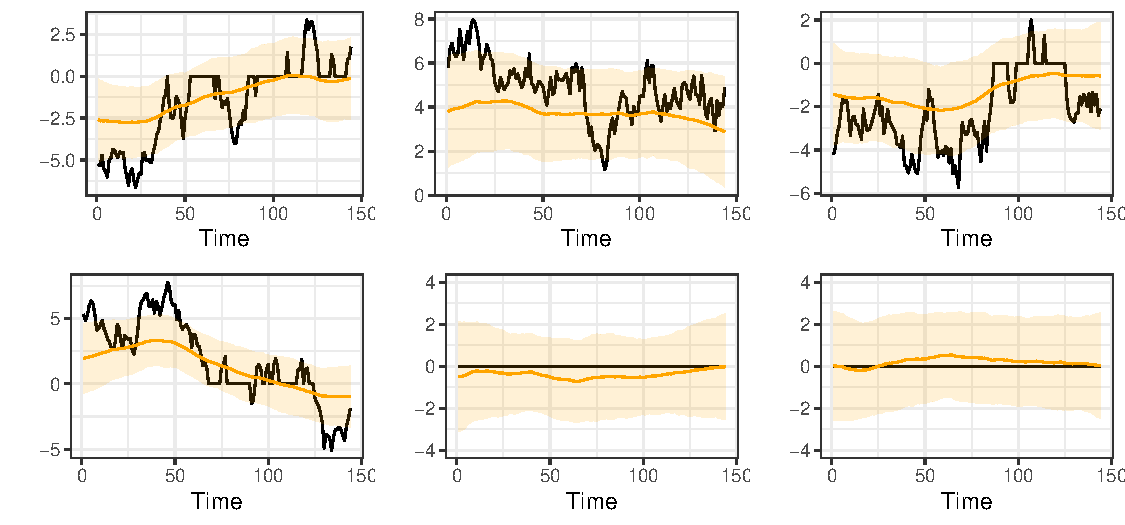
\includegraphics{Dynamic-Shrinkage-in-Bayesian-Structural-Time-Series-and-Vector-Autoregressive-Models_files/figure-latex/myfig2-1} 

}

\caption{Dynamic SSVS with $\Omega=1$ (no shrinkage) and discount factor model for the residuals; true values of $\beta_{1:T, j}$, $j=1, \ldots, 6$, (black) and smoothing estimates with 95 percent credible intervals (yellow) of the first six regression coefficients.}\label{fig:myfig2}
\end{figure}

Sparsity is induced by lowering the value of \(\Omega\). Indeed, Dynamic
SSVS with \(\Omega=0.2\) seems to lead to improved results. As shown in
Figure \ref{fig:myfig3}, the new model is able to capture more features
of the data. The smoothed values follow quite closely the true ones and
they present smaller credible intervals. Results may eventually improve
by choosing appropriate values for the hyperparameters
\((\Omega,\lambda_{1},\lambda_0,n_{0},d_{0},\delta)\). In this specific
case, we chose \(\lambda_{0}=0.01\) and \(\lambda_{1}=0.1\) in order to
maintain a good ratio between the spike and slab variances and hence to
facilitate the recognition of the active coefficients. Moreover, by
setting \(n_0=40\) and \(d_0=10\) we want to express our prior belief of
a small residual variance.

\begin{figure}[H]

{\centering 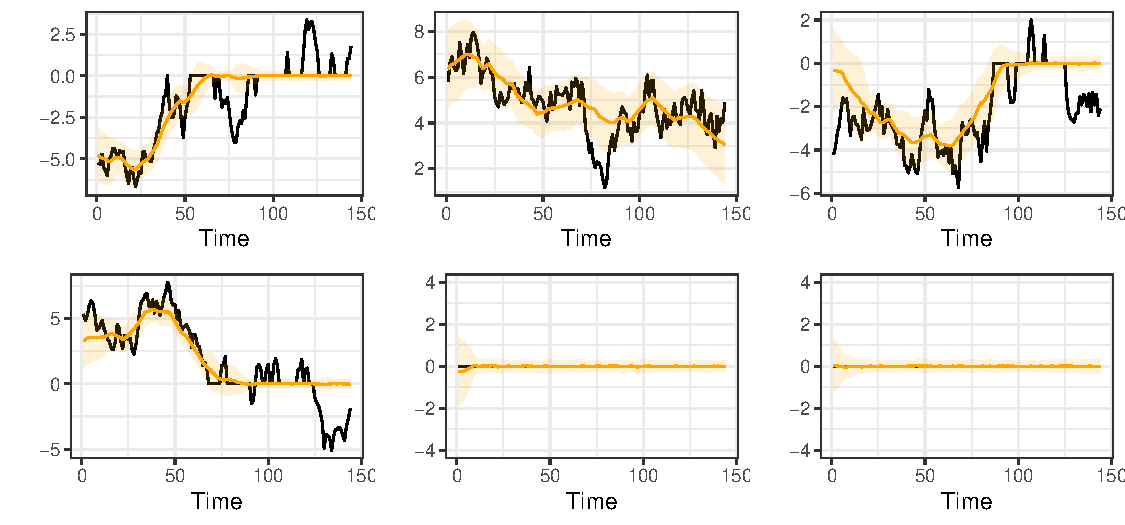
\includegraphics{Dynamic-Shrinkage-in-Bayesian-Structural-Time-Series-and-Vector-Autoregressive-Models_files/figure-latex/myfig3-1} 

}

\caption{Dynamic SSVS with $\Omega=0.2$ and discount factor model for the residuals; true values of $\beta_{1:T, j}$, $j=1, \ldots, 6$, (black) and smoothing estimates with 95 percent credible intervals (yellow) of the first six regression coefficients.}\label{fig:myfig3}
\end{figure}

As anticipated at the end of Section
\ref{Dynamic Stochastic Search Variable Selection}, estimates can
benefit from switching from a discount factor model to a stochastic
volatility model for the residual variances. We prove this statement by
comparing the Dynamic SSVS with these two alternative specifications.\\
Therefore, we replace the third step of Algorithm
\ref{alg:DSSVS-original} with the simulation strategy for stochastic
volatility models discussed in Section
\ref{A new proposal for the volatility process}. The parameters' priors
are \(\alpha_0\sim\mathcal{N}(-10,100)\),
\(\alpha_2\sim\mathcal{B}(20,1.5)\) and
\(\sigma^2_{\zeta}\sim\mathcal{IG}(0.5,0.5)\), and we set the
initialization values \(h_0^{(0)}=-2\), \(\alpha_0^{(0)}=-2\),
\(\alpha_1^{(0)}=0.9\) and \(\sigma_{\zeta}^{(0)}=0.1\). Figure
\ref{fig:myfig4} shows that there is an actual improvement when using a
stochastic volatility model for the residual variances. Indeed, this
model is less sensible to the ``spike trap'' we discussed in Section
\ref{Dynamic Stochastic Search Variable Selection}, as shown in Figure
\ref{fig:myfig5}.

\begin{figure}[H]

{\centering 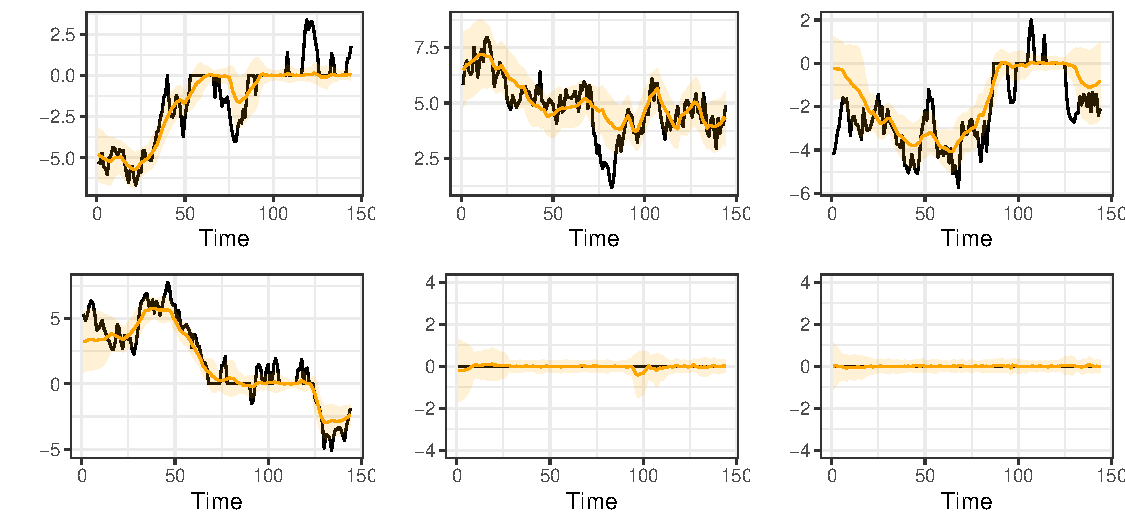
\includegraphics{Dynamic-Shrinkage-in-Bayesian-Structural-Time-Series-and-Vector-Autoregressive-Models_files/figure-latex/myfig4-1} 

}

\caption{Dynamic SSVS with $\Omega=0.2$ and stochastic volatility model for the residuals; true values of $\beta_{1:T, j}$, $j=1, \ldots, 6$, (black) and smoothing estimates with 95 percent credible intervals (yellow) of the first six regression coefficients.}\label{fig:myfig4}
\end{figure}

\begin{figure}[H]

{\centering 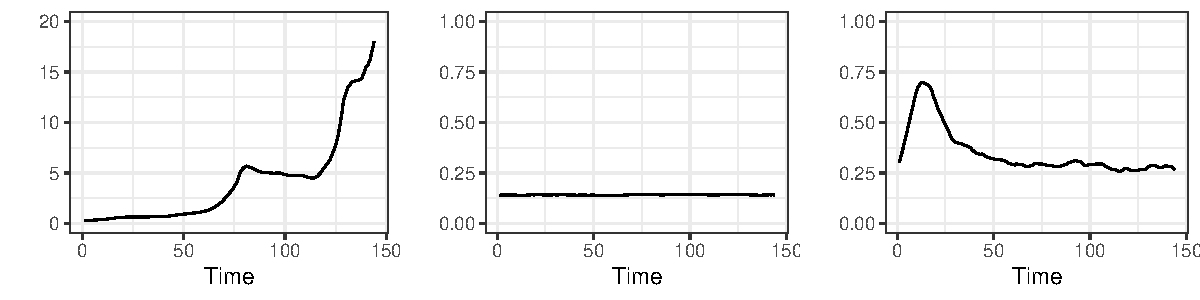
\includegraphics{Dynamic-Shrinkage-in-Bayesian-Structural-Time-Series-and-Vector-Autoregressive-Models_files/figure-latex/myfig5-1} 

}

\caption{MCMC variances' estimates of the volatility process with: a discount factor model (left panel), stochastic volatility model in a FFBS scheme (central panel) and a precision sampler scheme (right panel).}\label{fig:myfig5}
\end{figure}

\begin{figure}[H]

{\centering 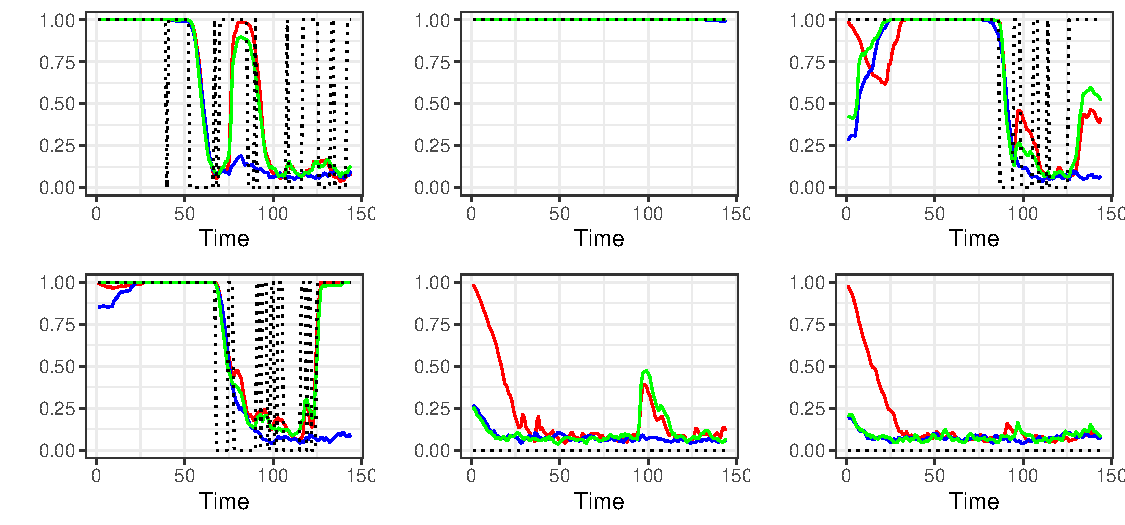
\includegraphics{Dynamic-Shrinkage-in-Bayesian-Structural-Time-Series-and-Vector-Autoregressive-Models_files/figure-latex/myfig12-1} 

}

\caption{MCMC approximation of the posterior inclusion probabilities of a Dynamic SSVS with: a discount factor model (blue line), stochastic volatility model in a FFBS scheme (green line) and a precision sampler scheme (red line). Black dotted line represents the true values.}\label{fig:myfig12}
\end{figure}

The running time of the simulation algorithms represents a limit when
these strategies have to be reiterated multiple times. This happens for
instance when one-step-ahead forecasts are generated for many periods
or, simply, when multiple estimations are performed in order to compare
results obtained with diverse specifications of the hypereparameters. By
replacing the FFBS step with a precision sampler, the running time
reduces while preserving performances as shown in Table
\ref{tab:mytab1}. However, the greatest enhancement in terms of running
time comes with the Dynamic EMVS. Therefore, here we present the results
obtained by fitting the data using a Dynamic EMVS both with a discount
factor model and with a stochastic volatility model. The initialization
value \(\boldsymbol{\beta}_{t}^{(0)}\) coincides with the least squares
estimates. Even though the original approach of
\protect\hyperlink{ref-rockova_mcalinn_2021}{Rockova and McAlinn}
(\protect\hyperlink{ref-rockova_mcalinn_2021}{2021a}) does not involve
least squares estimation for the initial values of the regression
coefficients, we notice that this simple trick can improve convergence.

\begin{figure}[H]

{\centering 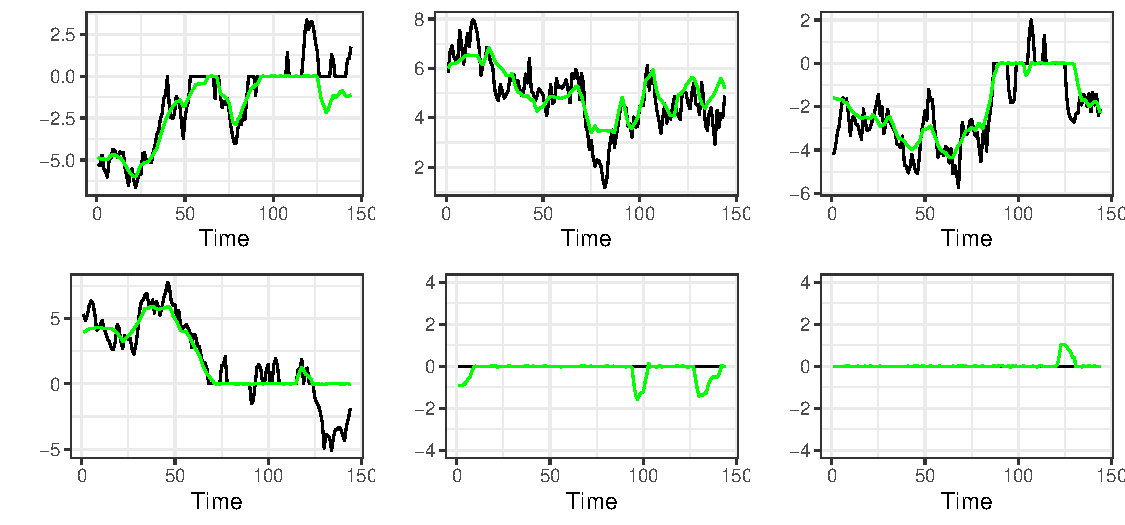
\includegraphics{Dynamic-Shrinkage-in-Bayesian-Structural-Time-Series-and-Vector-Autoregressive-Models_files/figure-latex/myfig9-1} 

}

\caption{Dynamic EMVS with discount factor model for the residual; true values of $\beta_{1:T, j}$, $j=1, \ldots, 6$, (black) and Maximum A Posteriori estimates (green) of the first six regression coefficients}\label{fig:myfig9}
\end{figure}

\begin{figure}[H]

{\centering 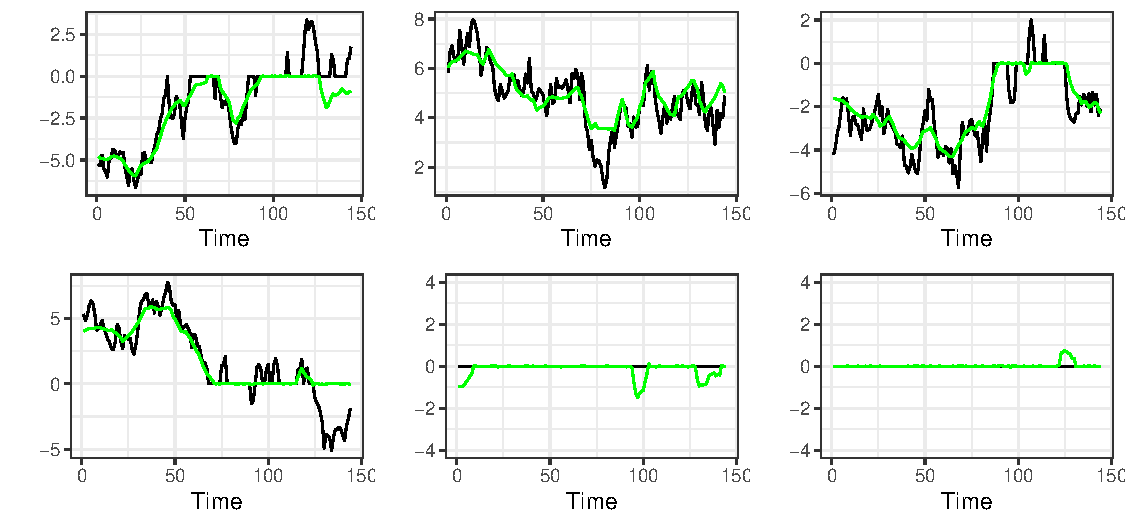
\includegraphics{Dynamic-Shrinkage-in-Bayesian-Structural-Time-Series-and-Vector-Autoregressive-Models_files/figure-latex/myfig10-1} 

}

\caption{Dynamic EMVS with stochastic volatility model for the residual; true values of $\beta_{1:T,j}$, $j=1, \ldots, 6$, (black) and Maximum A Posteriori estimates (green) of the first six regression coefficients }\label{fig:myfig10}
\end{figure}

\begin{figure}[H]

{\centering 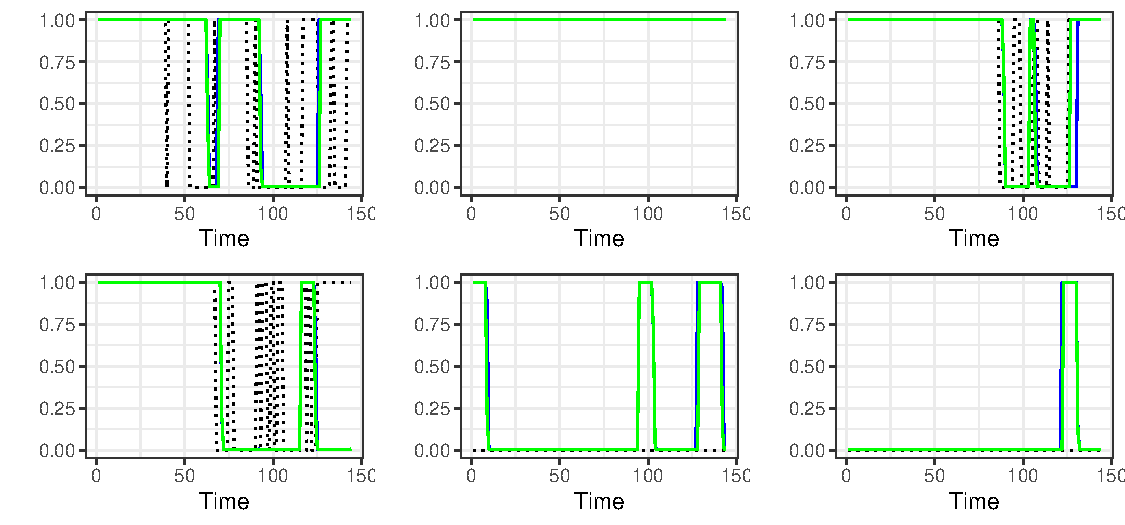
\includegraphics{Dynamic-Shrinkage-in-Bayesian-Structural-Time-Series-and-Vector-Autoregressive-Models_files/figure-latex/myfig13-1} 

}

\caption{Estimates of the conditional inclusion probabilities using Dynamic EMVS with: a discount factor model (blue line) and  a stochastic volatility model (green line). Black dotted line represents the true values.}\label{fig:myfig13}
\end{figure}

\begin{figure}[H]

{\centering 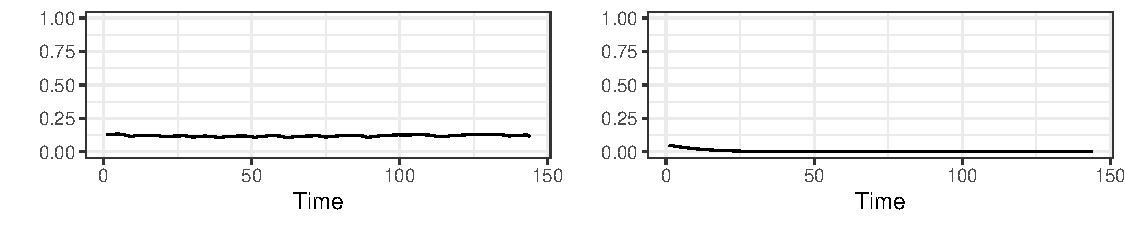
\includegraphics{Dynamic-Shrinkage-in-Bayesian-Structural-Time-Series-and-Vector-Autoregressive-Models_files/figure-latex/myfig11-1} 

}

\caption{Dynamic EMVS: variances' estimates of a stochastic volatility model (left panel) and discount factor model (right panel)}\label{fig:myfig11}
\end{figure}

Running times along with other meaningful information is presented in
Tables \ref{tab:mytab1} and \ref{tab:mytab2}. The metrics here used are:
the Sum of Squared Errors (SSE) between the actual and the estimated
state sequence, the Hamming distance (Ham) between the actual and the
estimated indicator vectors, the amount of total false negative (FN) and
false positive (FP), and the number of false detection (FD) and false
non detection (FND). In details, the Hamming Distance is a metrics used
in information theory to measure the number of substitutions necessary
to convert a string into another one. We use it to measure the distance
between the indicator vector estimated and the true one. More formally,
let \(\pi_{t,j}\equiv \mathbb{P}(\gamma_{t,j}=1|y_{1:T})\) (or
\(\pi_{t,j}=p^{\star}_{t,j}\) in the Dynamic EMVS case) and
\(\Pi=(\pi_{t,j})\), then \[
Ham(\Pi,\boldsymbol{\beta}_{0:T}^{0})=\sum_{j=1}^{p}\sum_{t=1}^{T}|\mathbb{I}(\pi_{t,j} \geq 0.5)-\mathbb{I}(\beta_{t,j}^{0}\neq 0)|
\] False positives and false negatives stands for the number of times in
which a coefficient is classified as relevant while it is not and vice
versa. On the other hand, false detection indicates the number of noise
covariates that are classified as relevant at least once over the whole
period whereas false non detection count the number of relevant
variables that have been ignored by the algorithm. The conclusion we
draw from Tables \ref{tab:mytab1} and \ref{tab:mytab2} are the
following. Firstly, without shrinkage (\(\Omega=1\)) the SSE is huge and
the model is clearly unable to fit the data. Therefore, the introduction
of a sparsity inducing strategy is necessary. Just by lowering
\(\Omega\) to 0.2 leads to great improvements. The Dynamic SSVS with
discount factor model provides in general the worst performances in
terms of SSE and it generates many false positive as a consequence of
the spike trap. On the other hand, the Dynamic SSVS with stochastic
volatility shows better performances. Moreover, replacing the FFBS with
a precision sampler implies minor accuracy of point estimates of the
very first observations. The large share of false positive reported in
Table \ref{tab:mytab1} can be explained from the fact that the latter
strategy assigns all the coefficient to the slab in the first periods
(see Figure \ref{fig:myfig13}). However, estimates improve for more
iterations of the Markov Chain. Overall, modelling variances as a
log-Normal AR(1) process proves to return better estimates of both
regression coefficients and the variance, for this reason we will
consider this specification as the baseline for developing further
models in the next chapters. In addition, the Dynamic EMVS represents a
valid alternative to the simulation algorithms. It provides indeed
precise point estimates at a reduced computational effort. However, one
should consider the fact that the deterministic nature of this algorithm
may result unsatisfactory whenever quantifying the uncertainty around
the estimates is of interest. Moreover, it shows a tendency to produce
false positives, therefore choosing the hyperparameters such that
shrinkage is more severe is recommended.

\begin{table}[H]

\caption{\label{tab:mytab1}Performance comparison}
\centering
\fontsize{10}{12}\selectfont
\begin{tabular}[t]{>{}ccccccccccc}
\toprule
Dynamic & Sampling Strategy & Volatility & $\Omega$ & Speed & SSE & Ham. & FP & FN & FD & FND\\
\midrule
 &  & DF & 1 & 745.56 & 2668.85 & 6754 & 6754 & 0 & 46 & 0\\
\cmidrule{3-11}
 &  & DF & 0.2 & 570.09 & 1031.947 & 127 & 19 & 108 & 0 & 0\\
\cmidrule{3-11}
 & \multirow[t]{-3}{*}{\centering\arraybackslash FFBS} & SV & 0.2 & 502.03 & 764.934 & 117 & 37 & 80 & 1 & 0\\
\cmidrule{2-11}
\multirow[t]{-4}{*}{\centering\arraybackslash SSVS} & Precision Sampler & SV & 0.2 & 251.27 & 1022.245 & 803 & 725 & 75 & 46 & 0\\
\cmidrule{1-11}
 &  & DF & 0.2 & 59.72 & 818.426 & 220 & 165 & 55 & 9 & 0\\
\cmidrule{3-11}
\multirow[t]{-2}{*}{\centering\arraybackslash EMVS} & \multirow[t]{-2}{*}{\centering\arraybackslash } & SV & 0.2 & 149.75 & 755.174 & 195 & 143 & 52 & 8 & 0\\
\bottomrule
\end{tabular}
\end{table}

\begin{table}[H]

\caption{\label{tab:mytab2}Assessing the estimation bias with focus on the first four predictors and on the remaining forty-six.}
\centering
\fontsize{10}{12}\selectfont
\begin{tabular}[t]{>{}cccccccc}
\toprule
\multicolumn{1}{c}{ } & \multicolumn{1}{c}{ } & \multicolumn{1}{c}{ } & \multicolumn{1}{c}{ } & \multicolumn{2}{c}{Predictors 1 to 4} & \multicolumn{2}{c}{Predictors 5 to 50} \\
\cmidrule(l{3pt}r{3pt}){5-6} \cmidrule(l{3pt}r{3pt}){7-8}
Dynamic & Sampling Strategy & Volatility & $\Omega$ & SSE & Ham. & SSE & Ham.\\
\midrule
 &  & DF & 1 & 1658.258 & 130 & 1010.593 & 6624\\
\cmidrule{3-8}
 &  & DF & 0.2 & 1027.37 & 127 & 4.577 & 0\\
\cmidrule{3-8}
 & \multirow[t]{-3}{*}{\centering\arraybackslash FFBS} & SV & 0.2 & 728.851 & 103 & 36.083 & 14\\
\cmidrule{2-8}
\multirow[t]{-4}{*}{\centering\arraybackslash SSVS} & Precision Sampler & SV & 0.2 & 723.891 & 102 & 298.354 & 701\\
\cmidrule{1-8}
 &  & DF & 0.2 & 688.124 & 101 & 130.301 & 119\\
\cmidrule{3-8}
\multirow[t]{-2}{*}{\centering\arraybackslash EMVS} & \multirow[t]{-2}{*}{\centering\arraybackslash } & SV & 0.2 & 659.006 & 95 & 96.168 & 100\\
\bottomrule
\end{tabular}
\end{table}

\section{Macroeconomic Data}

Inflation forecasting is probably the hardest challenge monetary policy
authorities face. What makes it a difficult tasks is that the price
growth can be explained by several factors, some of whom are not
directly observable. In general this factors are divided in some
macro-classes. Briefly, there are factors affecting demand which are
mainly due to fiscal and monetary policies and that are usually related
to the money supply, consumption, disposable income, public expenditure,
consumer expenditure, deficit financing, repayment of the public dept
and exports. Then there are factors affecting supply such as shortage of
important production factors, industrial disputes, natural calamities,
artificial scarcities and other international factors. In addition a
crucial role is played by agents' expectations which can be only
measured using proxies. In the current exercise, we decide to include
all the variables potentially affecting inflation in a unified
Time-Varying Parameter regression model. The approach is therefore more
data-driven and less theory-based. The purpose of this analysis (and the
following ones) is purely illustrative and it contains several
simplifications. Nonetheless, it also provides some good suggestions for
further, more accurate, economic analysis. Data on the variables
involved in this exercise are sourced from a large macroeconomic
database maintained by \protect\hyperlink{ref-FREDMD}{M. W. McCracken
and Ng} (\protect\hyperlink{ref-FREDMD}{2016}). The latter is primarily
based on Federal Reserve Economic Data (FRED)
\footnote{url: https://fred.stlouisfed.org/} and it contains seasonally
adjusted quarterly time series. Data are standardized and made
stationary through log-difference, with the exception of interests
rates. This transformations are in line with the instructions provided
by the authors of the database. The list of the \(40\) explanatory
variables involved in the analysis is reported in Appendix. The series
we are interested to forecast is the quarterly Price Consumption
Expenditure Price Index, which is commonly used as an indicator for
inflation. The model we estimate is \begin{align*}
y_{t+l}= & \mu_t+\boldsymbol{x}_{t}'\boldsymbol{\beta}_{t}+e^{\frac{h_t}{2}}\epsilon_{t}, \quad \epsilon_{t}\overset{iid}{\sim}\mathcal{N}(0,1) \\
\mu_t = & \phi_{1}\mu_{t-1}+\eta_{t}, \quad \eta_{t}\overset{iid}{\sim}\mathcal{N}(0,\lambda_1) \\
\boldsymbol{\beta}_{t} = & \Gamma_{t}\boldsymbol{\beta}_{t-1} + \boldsymbol{\xi}_{t}, \quad \boldsymbol{\xi}_{t}\sim\mathcal{N}(0,\Lambda_t) \\
h_{t}= & \alpha_0+\alpha_{1}(h_{t-1}-\alpha_{0})+\zeta_{t}, \quad \zeta_{t}\overset{iid}{\sim}\mathcal{N}(0,\sigma_{\zeta})
\end{align*} where \(l\) is 4 in the current analysis,
\(\Gamma_t=diag\{\gamma_{t,j}\phi_{1}\}_{j=1}^{p}\) and
\(\Lambda_{t}=diag\{\gamma_{t,j}\lambda_{1}+(1-\gamma_{t,j})\lambda_{0}\}_{j=1}^{p}\).
Moreover,
\(\gamma_{t,j}|\beta_{t-1,j}\overset{ind}{\sim}Bernoulli(\omega(\beta_{t-1,j}))\)
for \(j=1,\ldots,40\). The initial states are
\(\boldsymbol{\beta}_{0}\sim\mathcal{N}(\boldsymbol{m}_{0},\boldsymbol{C}_{0})\)
with \(\boldsymbol{m}_{0}=\boldsymbol{0}\) and
\(\boldsymbol{C}_{0}=diag\{\gamma_{0,j}\lambda_{1}/(1-\phi_{1}^{2})+(1-\gamma_{0,j})\lambda_{0}\}_{j=1}^{p}\)
and \(\mu_0\sim\mathcal{N}(0,\lambda_1)\). The priors of the stochastic
volatility model are the same of the simulation study. The model is
trained from 1968-12-01 to 2003-03-01, whereas one-step-ahead forecasts
are sequentially updated from 2003-06-01 to 2015-12-01. Out-of-sample
forecasts for the Dynamic SSVS are obtained by sampling
\(\gamma_{j,T+l}\) form a \(Bernoulli(\omega(\beta_{j,T}))\), and
\(h_{T+l}\) from
\(\mathcal{N}(\alpha_0+\alpha_1 h_{T},\sigma^{2}_{\zeta})\) and then
computing the one-step-ahead forecast mean \(f_{T+l}\) and the
one-step-ahead forecast variance \(q_{T+l}\) (using the notation of
Algorithm \ref{alg:DSSVS-original}) via a Kalman filter recursion. This
methodology for obtaining forecasts is applied by default to every
algorithm discussed in this thesis. However, for Dynamic EMVS the
parameters' means are replaced by their mode. In addition, predictive
performances are evaluated using a combination of four different
metrics. Three of them evaluate the forecast errors,
i.e.~\(e_{t}=y_{t}-f_{t}\), and they are: the Root Mean Squared Error
(RMSE), the Mean Absolute Scaled Error (MASE) and the Weighted Mean
Absolute Percentage Error (WMAPE). For the sake of clarity, the MASE is
computed in this way, \[
MASE=\frac{1}{n}\frac{\sum_{t=1}^{n}|y_{t}-f_{t}|}{\frac{1}{n-1}\sum_{t=2}^{n}|y_{t}-{y}_{t-1}|},
\] and it measures how well our model performs compared to a naive
forecast. Instead, the WMAPE is given by \[
WMAPE=\frac{\sum_{t=1}^{n}|y_{t}-f_{t}|}{\sum_{i=1}^{n}|y_{t}|}
\] and it represents an alternative to the classical MAPE which is
robust to the presence of zero or almost zero values. The forth metric
instead takes into account the entire predictive distribution and it is
the the sum of log predictive likelihoods (SLPL) defined as \[
SLPL = \sum_{t=1}^{n}\log \pi(y_{t}|f_{t},q_{t}).
\] For this exercise we use the Dynamic SSVS strategy with precision
sampler. The latter allows indeed for fast estimation without
sacrificing uncertainty. The time series of inflation is plotted in the
left panel of Figure \ref{fig:myfig001}. It clearly shows change points,
that can be captured by a Time-Varying Parameter model. Overall, the
residual standard deviations (central panel of Figure
\ref{fig:myfig001}) are low, indicating that the model has succeed in
selecting the right predictors, and it shows significant fluctuations
during shocking events. The very first estimates however are the less
reliable. The algorithm at first tends to assign all the coefficients to
the slab, but after a dozen of observations the estimates became more
precise and it starts to drop unimportant covariates from the model. In
every periods, about one quarter of the coefficients are active which
implies a significant improvements in terms of model interpret ability.
Moreover, this number usually increases during shocks or change points,
for then coming back to a value of around ten.

\begin{figure}[h]

{\centering 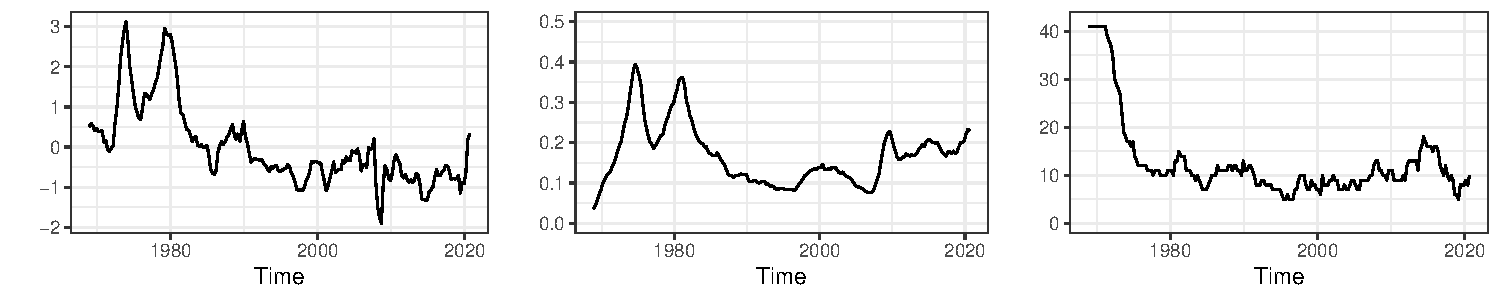
\includegraphics{Dynamic-Shrinkage-in-Bayesian-Structural-Time-Series-and-Vector-Autoregressive-Models_files/figure-latex/myfig001-1} 

}

\caption{Left panel: Time series of quarterly inflation recentred and rescaled. Middle: Evolution of residual standard deviations. Right panel: Number of active covariates that contribute in forecasting inflation.}\label{fig:myfig001}
\end{figure}

This in-sample assessment, that was useful to understand better the
general features of the time series, is then followed by the forecasting
exercise mentioned before. As shown in Figure \ref{fig:myfig002} dynamic
shrinkage plays an important role in reducing the forecast uncertainty.
The dynamic shrinkage model here used (\(\Omega=0.1\)) is able to
preserve the accuracy of the accuracy of the full model (\(\Omega=1\))
but it returns smaller credible intervals and therefore its point
estimates are more trustworthy from a statistical standpoint.

\begin{figure}[h]

{\centering 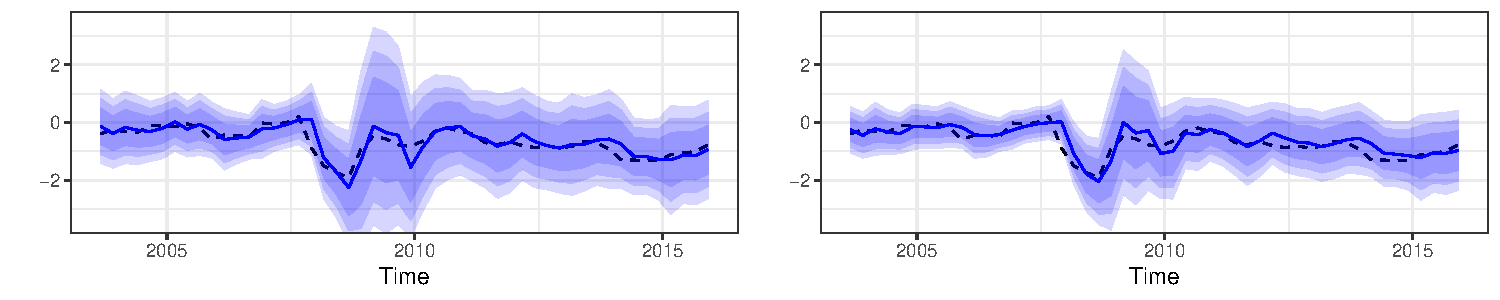
\includegraphics{Dynamic-Shrinkage-in-Bayesian-Structural-Time-Series-and-Vector-Autoregressive-Models_files/figure-latex/myfig002-1} 

}

\caption{One-step-ahead forecasts (blue line) with credible intervals and realizations (black dashed line). For similar point estimates, the model withouth shrinkage ($\Omega=1$) presents larger credible intervals than the model with actual dynamic shrinkage ($\Omega=0.1$).}\label{fig:myfig002}
\end{figure}

This visual insight is accompanied by a quantitative comparison in Table
\ref{tab:mytab001}. Here we compared several models characterized by
diverse intensity of shrinkage expressed by varying hyperparameter
\(\Omega\). In addition, we also compared models with different
specification of the AR(1) latent process. In details, while the metrics
based on forecast errors are almost equal, the SLPL reduces according to
\(\Omega\). And for the same value of \(\Omega\), the larger is
\(\phi_1\) (which must remain below 1 in absolute values) the better are
the forecasts. This results was to be expected. We want to preserve a
stationary structure of the latent process in order to maintain a stable
evolution of the inclusion probabilities \(\{w_t\}_{t=1}^{T}\), however
we want to also conserve the information gained on the model's parameter
from time to time. With an unjustified low value of \(\phi_1\) the past
history of the coefficient become uninformative to determine the value
of the regression coefficient in \(t\), making the estimation task
harder.

\begin{table}[H]

\caption{\label{tab:mytab001}Performance comparison for varying intensities of shrinkage}
\centering
\begin{tabular}[t]{cccccc}
\toprule
$\Omega$ & $\phi_1$ & RMSE & WMAPE & MASE & SLPL\\
\midrule
1.0 & 0.98 & 0.264 & 0.287 & 1.021 & -24.113\\
\cmidrule{1-6}
0.9 & 0.98 & 0.261 & 0.285 & 1.011 & -23.790\\
\cmidrule{1-6}
0.7 & 0.98 & 0.261 & 0.287 & 1.019 & -21.798\\
\cmidrule{1-6}
0.5 & 0.98 & 0.263 & 0.286 & 1.016 & -19.450\\
\cmidrule{1-6}
0.3 & 0.98 & 0.264 & 0.289 & 1.027 & -17.453\\
\cmidrule{1-6}
 & 0.98 & 0.263 & 0.291 & 1.033 & -14.708\\
\cmidrule{2-6}
 & 0.80 & 0.305 & 0.351 & 1.247 & -19.209\\
\cmidrule{2-6}
 & 0.40 & 0.533 & 0.662 & 2.353 & -40.135\\
\cmidrule{2-6}
\multirow[t]{-4}{*}{\centering\arraybackslash 0.1} & 0.10 & 0.755 & 0.951 & 3.378 & -78.036\\
\bottomrule
\end{tabular}
\end{table}

\chapter[Bayesian Structural Time Series]{Dynamic Shrinkage in Bayesian Structural Time Series}\label{Dynamic Shrinkage in Bayesian Structural Time Series}

Building on the results of the previous chapter, we want to propose a
new class of models for time series analysis. It consists of an
extension of the Bayesian Structural Time Series models developed by
\protect\hyperlink{ref-scott_varian_2013}{Scott and Varian}
(\protect\hyperlink{ref-scott_varian_2013}{2013}). Starting from this
framework we develop a BSTS model with both Dynamic Spike-and-Slab
process priors and stochastic volatility. This model can be also
regarded as an extension of the TVP regression model defined in equation
(\ref{eq:eq211}) that takes into account also structural time series
components such as seasonality and trend. These features are indeed
usually exhibited by many time series, especially in macroeconomics, and
including them inside the model can improve forecasting performances.\\
The model is defined by the following system of equations:
\begin{equation}
   \begin{aligned}\label{eq:dssbsts1}
  y_{t} = & \mu_{t}+\tau_{t}+\boldsymbol{x}'_{t}\boldsymbol{\beta}_{t}+\epsilon_{t},\\
  \mu_{t} = & \mu_{t-1}+\delta_{t-1}+u_{t},\\
  \delta_{t} = & \delta_{t-1}+v_{t},\\
  \tau_{t} = & -\sum_{s=1}^{S-1}\tau_{t-s}+w_{t}, \\
  \boldsymbol{\beta}_{t} = & \Gamma_{t}\boldsymbol{\beta}_{t-1} + \boldsymbol{\xi}_{t} 
  \end{aligned}
  \end{equation} where the \(p\) coefficients are independent and
identically distributed according to DSS priors:
\(\beta_{1:T,j}\overset{iid}{\sim}DSS(\Omega,\lambda_{0},\lambda_1,\phi_0,\phi_1)\)
for \(j=1,\ldots,p\). In addition, given the results illustrated in the
previous chapter, that suggest improvements with an AR(1) stochastic
volatility model, we model the residuals using following specification
\(\epsilon_t\sim\mathcal{N}(0,e^{h_{t}})\) with
\begin{equation}\label{eq:dssbsts2}
h_{t}=\alpha_{0}+\alpha_{1}(h_{t-1}-\alpha_{0})+\zeta_{t}
\end{equation} The disturbances \(u_{t}\), \(v_{t}\), \(w_{t}\) and
\(\zeta_{t}\) are i.i.d. normally distributed with mean zero and
variances respectively \(\sigma^{2}_{\mu}\), \(\sigma^{2}_{\delta}\),
\(\sigma^{2}_{\tau}\) and \(\sigma^{2}_{\zeta}\). Ideally, it would be
possible to estimate these variances by maximum likelihood or assigning
an Inverse-Gamma prior to them and proceeding with Bayesian inference.
However, there are some identifiability issues in separating the
residuals of the trend, the slope and the seasonality, and the MLE or
MCMC may fail at converging towards a unique solution. We do not have
this problem since we set a-priori
\(\sigma^{2}_{\mu}=\sigma^{2}_{\delta}=\sigma^{2}_{\tau}=\lambda_1\) in
the applications discussed in this thesis, where \(\lambda_1\) is a
predetermined scalar. On the other hand,
\(\sigma^{2}_{\zeta}\sim\mathcal{IG}(0.5,0.5)\). Such choice is
convenient since it is the default prior for \(\sigma^{2}_{\zeta}\) used
in the \texttt{stochvol} R-package. Moreover, in the state equation for
\(\boldsymbol{\beta}_t\),
\(\Gamma_t=diag\{\gamma_{t,j}\phi_{1}\}_{j=1}^{p}\) and
\[ \boldsymbol{\xi}_{t} \overset{iid}{\sim}\mathcal{N}(0,\Lambda_t)\; \mbox{with} \; \Lambda_{t}=diag\{\gamma_{t,j}\lambda_{1}+(1-\gamma_{t,j})\lambda_{0}\}_{j=1}^{p}. \]
Let us recall that
\(\gamma_{t,j}|\beta_{t-1,j}\overset{ind}{\sim}Bernoulli(\omega(\beta_{t-1,j}))\)
for \(j=1,\ldots,p\). The values of \(\lambda_{0}\) and \(\lambda_{1}\)
play a crucial role in ensuring that the estimation strategy is able to
effectively distinguish the signal from the noise. Usually, some
preliminary estimations have to be performed to understand which values
of \(\lambda_{0}\) and \(\lambda_{1}\) provide the best fitting of the
data. Overall, it is recommended to maintain the ratio
\(\lambda_1/\lambda_0=10\).\\
The DLM representation of the Bayesian Structural Time Series is very
useful since it allows to take advantage of the Kalman filter formulas,
however some considerations are necessary. Firstly, the state vector is
\(\boldsymbol{\theta}_{t}=(\mu_{t},\delta_{t},\tau_{t},\tau_{t-1},...,\tau_{t-S+1},\boldsymbol{\beta}_{t})'\).
Consequently, \(\boldsymbol{F}_{t}=(1,0,1,0,...,0,\boldsymbol{x}_{t})\)
and
\(\boldsymbol{G}_{t}=blockdiag(\boldsymbol{G}_{t}^{(trend)},\boldsymbol{G}_{t}^{(seasonal)},\Gamma_{t})\)
where

\[
\boldsymbol{G}_{t}^{(trend)}=\begin{pmatrix} 
1 & 1\\
0 & 1      
\end{pmatrix} \quad \text{and} \quad \boldsymbol{G}_{t}^{(seasonal)}=\begin{pmatrix}
-1 & -1 & ... & -1 \\
1 & 0 & ...& 0 \\
0 & 1 & ... & 0 \\
\vdots & \vdots & \ddots & \vdots \\
0 & 0 & ... & 1
\end{pmatrix}.
\] The specification of \(\boldsymbol{G}_{t}^{(seasonal)}\) is a direct
consequence of the identifiability constraint on the seasonal factors,
i.e.~\(\sum_{s=1}^{S}\tau_{s}=0\). Similarly,
\(\Sigma_{\eta,t}=blockdiag(\Sigma_{\eta,t}^{(trend)},\boldsymbol{\Sigma}_{\eta,t}^{(seasonal)},\Lambda_{t})\)
where \[
\Sigma_{\eta,t}^{(trend)}=\begin{pmatrix} 
\sigma^{2}_{\mu} & 0\\
0 & \sigma^{\delta}      
\end{pmatrix} \quad \text{and} \quad \Sigma_{\eta,t}^{(seasonal)}=\begin{pmatrix}
\sigma^{t}_{\tau} & 0 & ... & 0 \\
0 & 0 & ...& 0 \\
0 & 0 & ... & 0 \\
\vdots & \vdots & \ddots & \vdots \\
0 & 0 & ... & 0
\end{pmatrix}.
\] In addition, nothing prevents the model to accommodate also a static
regression component \(\boldsymbol{z}_t'\boldsymbol{\beta}\). This can
be accomplished in several ways, however the most convenient from a
computational point of view is the one envisaged by
\protect\hyperlink{ref-scott_varian_2013}{Scott and Varian}
(\protect\hyperlink{ref-scott_varian_2013}{2013}) that consists in
consists in appending a constant 1 to the state vector and
\(\boldsymbol{z}_{t}'\boldsymbol{\beta}\) to \(\boldsymbol{F}_t\) in
this way:
\(\boldsymbol{\theta}_{t}=(1,\mu_{t},\delta_{t},\tau_{t},\tau_{t-1},...,\tau_{t-S+1},\boldsymbol{\beta}_{t})'\)
and
\(\boldsymbol{F}_{t}=(\boldsymbol{z}_{t}'\boldsymbol{\beta},1,0,1,0,...,0,\boldsymbol{x}_{t})\).\\
Efficient posterior sampling is provided by the Dynamic SSVS we
introduced in the Section
\ref{Dynamic Stochastic Search Variable Selection} with some
modifications due to the introduction of structural components. All the
steps are summarized in Algorithm \ref{alg:DSSBSTS} and we refer to
Section \ref{Dynamic Stochastic Search Variable Selection} for further
details. Note that the expansion of the state vector's size due to
structural components leads inevitably to a slower running time since
the Kalman filter's computational complexity is linear in data length
but quadratic in the state vector dimension. Considering for instance
quarterly data, \(\boldsymbol{\theta}_{t}\) becomes a column vector of
\(p\) regression coefficients plus \(3\) seasonal components and \(2\)
trend components. Therefore, in order to reduce computational efforts,
we also propose an extension of the Dynamic EMVS seen in Section
\ref{Dynamic EMVS} for this novel BSTS model. The latter results to be
particularly useful for exploratory analysis, when multiple attempts are
performed to find satisfying values of the hyperparameters.

\begin{algorithm}
\caption{Dynamic SSVS in BSTS with Stochastic Volatility} \label{alg:DSSBSTS}
\nl \textbf{Initialize} $\gamma_{j,t}$ and $\sigma_{\epsilon,t}$ for $0 \leq t \leq T$ and $1 \leq j \leq p$ and set $n_{0}$ and $d_{0}$\;
\begin{center}
\emph{Step 1: Sample Time Series Structural Components}\\
\end{center}
\nl \For{$1 \leq t \leq T$}{ 
Compute $\boldsymbol{a}_{t}=\boldsymbol{G}_{t}\boldsymbol{m}_{t-1}$\;
Compute $\boldsymbol{R}_{t}=\boldsymbol{G}_{t}\boldsymbol{C}_{t-1}\boldsymbol{G}'_{t}+\Sigma_{\eta,t}$\;
Compute $f_{t}=\boldsymbol{F}'_{t}\boldsymbol{a}_{t}$ and $e_{t}=y_{t}-f_{t}$\;
Compute $q_{t}=\boldsymbol{F}'_{t}\boldsymbol{R}_{t}\boldsymbol{F}_{t}+\sigma^{2}_{\epsilon,t}$\;
Compute $\boldsymbol{m}_{t}=\boldsymbol{a}_{t}+\boldsymbol{A}_{t}e_{t}$ and $\boldsymbol{C}_{t}=\boldsymbol{R}_{t}-\boldsymbol{A}_{t}\boldsymbol{A}'_{t}q_{t}$ with $\boldsymbol{A}_{t}=\boldsymbol{R}_{t}\boldsymbol{F}_{t}/q_{t}$
}
Draw $\boldsymbol{\theta}_{t}\sim \mathcal{N}(\boldsymbol{m}_{T},\boldsymbol{C}_{t})$\; \For{$t = T-1,...,0$}{  
Compute $\boldsymbol{a}_{T}(t-T)=\boldsymbol{m}_{t}+\boldsymbol{B}_{t}(\boldsymbol{\theta}_{t+1}-\boldsymbol{a}_{t+1})$\;
Compute $\boldsymbol{R}_{t}(t-T)=\boldsymbol{C}_{t}-\boldsymbol{B}_{t}\boldsymbol{R}_{t+1}\boldsymbol{B}'_{t}$ where $\boldsymbol{B}_{t}=\boldsymbol{C}_{t}\boldsymbol{G}'_{t+1}\boldsymbol{R}_{t+1}^{-1}$\;
Draw $\boldsymbol{\theta}_{t}\sim \mathcal{N}(\boldsymbol{a}_{T}(t-T),\boldsymbol{R}_{t}(t-T))$ \;
}
\begin{center}
\emph{Step 2: Sample Indicators}\\
\end{center}
\nl \For{$j=1,...,p$}{
\For{$1 \leq t \leq T$}{
Compute $\omega_{j,t}=\omega(\beta_{j,t-1})$ from \;
Compute $p^{\star}_{t,j}=p^{\star}_{t,j}(\beta_{j,t})$ from \;
Draw $\gamma_{j,t} \sim Bernoulli(p^{\star}_{j,t}(\beta_{j,t}))$\;
}
Compute $p^{\star}_{j,0}=\omega(\beta_{j,0})$\;
Draw $\gamma_{j,0} \sim Bernoulli(p^{\star}_{j,0}(\beta_{j,0}))$\;
}
\begin{center}
\emph{Step 3: Sample Volatility}\\
\end{center}
\nl Compute $r_{t}=y_{t}-\boldsymbol{F}_{t}'\boldsymbol{\theta}_{t}$ for $t=1,...,T$\;
Sample $(h_{0},...,h_{T})$ using the efficient sampling strategy described in Section \ref{A new proposal for the volatility process}\;
Compute $\sigma^{2}_{\epsilon,t}=e^{h_{t}}$\;
\end{algorithm}

\section{Dynamic Expectation-Maximization Variable Selection}

The huge computational saving in running time through the Dynamic EMVS
encouraged us to develop a modified version of the strategy of
\protect\hyperlink{ref-rockova_mcalinn_2021}{Rockova and McAlinn}
(\protect\hyperlink{ref-rockova_mcalinn_2021}{2021a}) that takes into
account also structural time series components. Here, the MAP trajectory
to be approximated is
\(\hat{\boldsymbol{\theta}}_{1:T}=\arg\max \pi(\boldsymbol{\beta}_{1:T},\mu_{1:T},\delta_{1:T},\tau_{1:T}\mid y_{1:T})\).
Fortunately, the considerations done previously for the E-step in the
previous chapter still hold. However, the M-step requires instead
further computations. Here we describe how to implement the Dynamic EMVS
for quarterly data, nonetheless the following steps can be generalized
for other data frequencies.\\
The joint density prior is factorized as it follows \begin{align*}
 \pi(\mu_{0:T},\delta_{0:T},\tau_{0:T},&\boldsymbol{\beta}_{0:T},\boldsymbol{\gamma}_{0:T},\sigma^{2}_{\epsilon,0:T}) = \pi(\mu_{0})\pi(\delta_{0})\pi(\tau_{0})\pi(\boldsymbol{\beta}_{0}|\boldsymbol{\gamma}_{0})\pi(\boldsymbol{\gamma}_{0})... \\ 
...\prod_{t=1}^{T}\bigg\{ & \pi(\sigma^{2}_{\epsilon,t}\mid\sigma^{2}_{\epsilon,t-1})\pi(\mu_{t}\mid\mu_{t-1},\delta_{t-1})\pi(\delta_{t}\mid\delta_{t-1})\pi(\tau_{t}\mid\tau_{t-1},\tau_{t-2},\tau_{t-3})... \\
& ... \prod_{j=1}^{p}\bigg[\pi(\beta_{t,j}\mid\gamma_{t,j},\beta_{t-1,j})\pi(\gamma_{t,j}\mid\beta_{t-1,j})\bigg]\bigg\}
\end{align*} whose posterior can be decomposed as \begin{align*}
& \pi(\mu_{0:T},\delta_{0:T},\tau_{0:T},\boldsymbol{\beta}_{0:T},\boldsymbol{\gamma}_{0:T},\sigma^{2}_{\epsilon,0:T}\mid y_{1:T}) \propto \\ & \pi(y_{1:T}\mid \mu_{0:T},\delta_{0:T},\tau_{0:T},\boldsymbol{\beta}_{0:T},\boldsymbol{\gamma}_{0:T},\sigma^{2}_{\epsilon,0:T})\pi(\mu_{0:T},\delta_{0:T},\tau_{0:T},\boldsymbol{\beta}_{0:T},\boldsymbol{\gamma}_{0:T},\sigma^{2}_{\epsilon,0:T}).
\end{align*} Therefore, in logs, we have \begin{align*}
& \log\pi(\mu_{0:T},\delta_{0:T},\tau_{0:T},\boldsymbol{\beta}_{0:T},\boldsymbol{\gamma}_{0:T},\sigma^{2}_{\epsilon,0:T}\mid y_{1:T}) =\\
& C - \frac{(\mu_{0}-m_{0}^{(\mu)})^{2}}{2C_{0}^{(\mu)}}- \frac{(\delta_{0}-m_{0}^{(\delta)})^{2}}{2C_{0}^{(\delta)}}- \frac{(\tau_{0}-m_{0}^{(\tau)})^{2}}{2C_{0}^{(\tau)}} \\
& - \sum_{j=1}^{p}\bigg\{\gamma_{0,j}\frac{\beta_{0,j}^{2}(1-\phi_{1}^{2})}{2\lambda_{1}}+(1-\gamma_{0,j})\frac{\beta_{0,j}^{2}}{2\lambda_{0}}-\gamma_{0,j}\log\Theta-(1-\gamma_{0,j})\log(1-\Theta)\bigg\} \\
& +\sum_{t=1}^{T}\sum_{j=1}^{p}[\gamma_{t,j}\log \theta_{t,j}+(1-\gamma_{t,j})\log(1-\theta_{t,j})] \\
& - \sum_{t=1}^{T}\bigg\{\frac{(y_{t}-\boldsymbol{x}_{t}'\boldsymbol{\beta}_{t}-\mu_{t}-\tau_{t})^{2}}{2\sigma^{2}_{\epsilon,t}}+\sum_{j=1}^{p}\bigg[\gamma_{t,j}\frac{(\beta_{t,j}-\phi_{1}\beta_{t-1,j})^{2}}{2\lambda_{1}}+(1-\gamma_{t,j})\frac{\beta_{t,j}^{2}}{2\lambda_{0}}\bigg]+\\
& \log\pi(\sigma^2_{\epsilon,t}|\sigma^2_{\epsilon,t-1})+\frac{(\mu_{t}-\mu_{t-1}-\delta_{t-1})^{2}}{2\sigma^{2}_{\mu}}+\frac{(\delta_{t}-\delta_{t-1})^{2}}{2\sigma^{2}_{\delta}}+\frac{(\tau_{t}+\tau_{t-1}+\tau_{t-2}+\tau_{t-3})^{2}}{2\sigma^{2}_{\tau}} \bigg\}.
\end{align*} Maximizing
\(\mathbb E(\mu_{0:T},\delta_{0:T},\tau_{0:T},\boldsymbol{\beta}_{0:T},\boldsymbol{\gamma}_{0:T},\sigma^{2}_{\epsilon,0:T}\mid y_{1:T})=Q(\boldsymbol{\Xi}\mid y_{1:T})\)
with respect to
\((\mu_{0:T},\delta_{0:T},\tau_{0:T},\boldsymbol{\beta}_{0:T})\), one
obtains the following first order conditions: \begin{align*}
\frac{\partial Q(\boldsymbol{\Xi}\mid y_{1:T})}{\partial \tau_{t}}  & = 0 \iff \\
\tau_{t} =\bigg(\frac{4}{\sigma^{2}_{\tau}}+ & \nu^{\star}\bigg)^{-1}\bigg\{\frac{1}{\sigma^{2}_{\tau}}(-3\tau_{t-1}-2\tau_{t-2}-\tau_{t-3}-3\tau_{t+1}-2\tau_{t+2}-\tau_{t+3})+\nu^{\star}(y_{t}-\boldsymbol{x}_{t}'\boldsymbol{\beta}_{t}-\mu_{t}))\bigg\} \\
 \frac{\partial Q(\boldsymbol{\Xi}\mid y_{1:T})}{\partial \tau_{0}} & = 0 \iff
 \tau_{0} = \bigg(\frac{1}{C_{0}^{(\tau)}}+\frac{1}{\sigma^{2}_{\tau}}\bigg)^{-1}\bigg\{\frac{m_{0}^{(\tau)}}{C_{0}^{(\tau)}}-\frac{1}{\sigma^{2}_{\tau}}(3\tau_{1}+2\tau_{2}+\tau_{3})\bigg\} \\
 \frac{\partial Q(\boldsymbol{\Xi}\mid y_{1:T})}{\partial \delta_{t}} & = 0 \iff  \delta_{t} =\bigg(\frac{1}{\sigma^{2}_{\mu}}+\frac{2}{\sigma^{2}_{\delta}}\bigg)^{-1}\bigg\{\frac{1}{\sigma^{2}_{\mu}}(\mu_{t+1}-\mu_{t})+\frac{1}{\sigma^{2}_{\delta}}(\delta_{t-1}+\delta_{t+1})\bigg\} \\
\frac{\partial Q(\boldsymbol{\Xi}\mid y_{1:T})}{\partial \delta_{0}} & = 0 \iff  \delta_{0}=\bigg(\frac{1}{C_{0}^{(\delta)}}+\frac{1}{\sigma^{2}_{\mu}}+\frac{1}{\sigma^{2}_{\delta}}\bigg)^{-1}\bigg\{\frac{m_{0}^{(\delta)}}{C_{0}^{(\delta)}}+\frac{1}{\sigma^{2}_{\mu}}(\mu_{1}-\mu_{0})+\frac{1}{\sigma^{2}_{\delta}}\delta_{1}\bigg\} \\
\frac{\partial Q(\boldsymbol{\Xi}\mid y_{1:T})}{\partial \mu_{t}} & = 0 \iff
\mu_{t} = \bigg(\frac{2}{\sigma^{2}_{\mu}}+\nu^{\star}\bigg)^{-1}\bigg\{\frac{1}{\sigma^{2}_{\mu}}(\mu_{t+1}-\mu_{t-1}+\delta_{t-1}-\delta_{t})+\nu^{\star}(y_{t}-\boldsymbol{x}_{t}'\boldsymbol{\beta}_{t}-\tau_{t})\bigg\} \\
\frac{\partial Q(\boldsymbol{\Xi}\mid y_{1:T})}{\partial \mu_{0}} & = 0 \iff 
\mu_{0} = \bigg(\frac{1}{\sigma^{2}_{\mu}}+\frac{1}{C_{0}^{(\mu)}}\bigg)^{-1}\bigg\{\frac{m_{0}^{(\mu)}}{C_{0}^{(\mu)}}+\frac{\mu_{1}}{\sigma^{2}_{\mu}}-\frac{\delta_{0}}{\sigma^{2}_{\mu}}\bigg\} \\
\frac{\partial Q(\boldsymbol{\Xi}\mid y_{1:T})}{\partial \boldsymbol{\beta}_{t}} & = 0 \iff \boldsymbol{\beta}_{t} = \boldsymbol{D}_{t}^{-1}\bigg\{\nu^{\star}(y_{t}-\mu_{t}-\tau_{t})\boldsymbol{x}_{t}+\frac{\phi_1}{\lambda_1}\boldsymbol{\beta}_{t-1}\odot\boldsymbol{p}^{\star}_{t}+\frac{\phi_1}{\lambda_{1}}\boldsymbol{\beta}_{t+1}\odot\boldsymbol{p}^{\star}_{t+1}\bigg\} \\
\frac{\partial Q(\boldsymbol{\Xi}\mid y_{1:T})}{\partial \boldsymbol{\beta}_{0}} & = 0 \iff
\boldsymbol{\beta}_{0}=\boldsymbol{D}_{0}^{-1}\frac{\phi_1}{\lambda_1}\boldsymbol{\beta_1}\odot\boldsymbol{p_{1}^{\star}}
\end{align*} where \[
\boldsymbol{D}_t=\frac{\boldsymbol{x}_{t}\boldsymbol{x}_{t}'}{\sigma^{2}_{\epsilon,t}}+diag\bigg\{\frac{p^{\star}_{t,j}}{\lambda_1}+\frac{1-p^{\star}_{t,j}}{\lambda_{0}}+\frac{\phi^{2}_{1}p^{\star}_{t+1,j}}{\lambda_{1}}\bigg\}_{j=1}^{p}
\] and \[
\boldsymbol{D}_0=diag\bigg\{\frac{(1-\phi^2_1)p^{\star}_{0,j}}{\lambda_1}+\frac{1-p^{\star}_{0,j}}{\lambda_0}+\frac{\phi^{2}_1 p^{\star}_{1,j}}{\lambda_1}\bigg\}_{j=1}^{p}
\] Again, the Woodburry formula simplifies calculations and reduces
running time. The first order conditions listed above vary for
\(t=\{0,T\}\). For instance, the argmax with respect to \(\tau_T\) is
\[\tau_{T}=\bigg(\frac{1}{\sigma^{2}_{\tau}}+\nu^{\star}\bigg)^{-1}\bigg\{\frac{1}{\sigma^{2}_{\tau}}(-\tau_{T-1}-\tau_{T-2}-\tau_{T-3})+\nu^{\star}(y_{T}-\boldsymbol{x}_{T}'\boldsymbol{\beta}_{T}-\mu_{T}))\bigg\}
\] and so on. In the next section we explore the potential of the
proposed model for structural time series in a simulation study.

\section{Simulation Study}\label{SD2}

In order to illustrate of the validity of this novel approach, we
propose a toy example on quasi-synthetic data. It is possible to
generate a Bayesian Structural Time Series easily by summing up two or
more processes. Therefore we generate synthetic data from a TVP
regression model with \(p=20\) explanatory variables of which the first
four predictors affect the outcome whereas the remaining \(16\)
predictors are just disturbing factors following the same steps
illustrated in Section \ref{SD}. For this simulation study, we want to
also include a trend and a seasonal component. To this aim, rather than
generating synthetic data, I used a time series already available in R,
namely the series ``AirPassengers'' (the classic Box and Jenkins airline
data consisting of monthly totals of international airline passengers
from 1949 to 1960), which shows a trend and a multiplicative
seasonality. The data used in the simulation study is obtained as the
composition of the synthetis data plus the log of the series
AirPassengers, as shown in Figure \ref{fig:myfig6}. Note, we rescale the
data to emphasize its structural features.

\begin{figure}[H]

{\centering 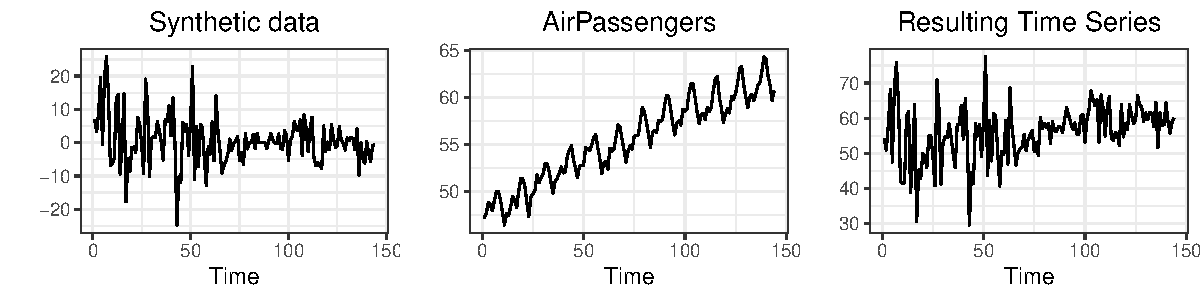
\includegraphics{Dynamic-Shrinkage-in-Bayesian-Structural-Time-Series-and-Vector-Autoregressive-Models_files/figure-latex/myfig6-1} 

}

\caption{Left panel: Synthetic data generated from a TVP regression model. Middle: Rescaled Logarithmic AirPassengers. Right panel: Resulting time series used in the simulation.}\label{fig:myfig6}
\end{figure}

Clearly, fitting the resulting time series is anything but easy and this
is also the reason why we restricted the number of (potential)
regressors to 20 (rather than 50 as in Section \ref{SD}). Moreover,
another reason fro limiting the simulation study to a moderate number of
regressors is the size of the state vector, that here includes the
structural components. For instance, using (dynamic) seasonal factors,
\(13\) additional latent states have to be estimated. Two of them are
the time-varying trend with stochastic slope, whereas the remaining
eleven represent the seasonality. Nevertheless, Dynamic SSVS and Dynamic
EMVS prove to be able to capture the source of the signal. This is shown
in Figure \ref{fig:myfig7} and \ref{fig:myfig8} and in particular in the
table below.

\begin{figure}[ht]

{\centering 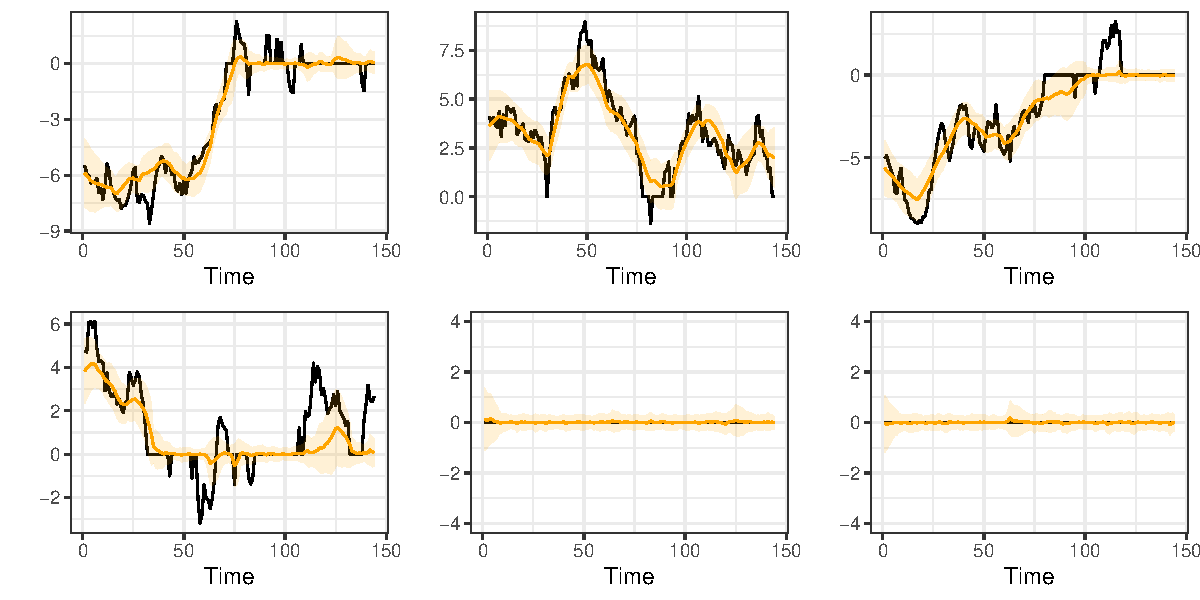
\includegraphics{Dynamic-Shrinkage-in-Bayesian-Structural-Time-Series-and-Vector-Autoregressive-Models_files/figure-latex/myfig7-1} 

}

\caption{Dynamic SSVS for BSTS model; true values of $\beta_{1:T, j}$, $j=1, \ldots, 6$, (black) and smoothed estimates with 95 percent credible intervals (yellow) of the first six regression coefficients.}\label{fig:myfig7}
\end{figure}

\begin{figure}[h]

{\centering 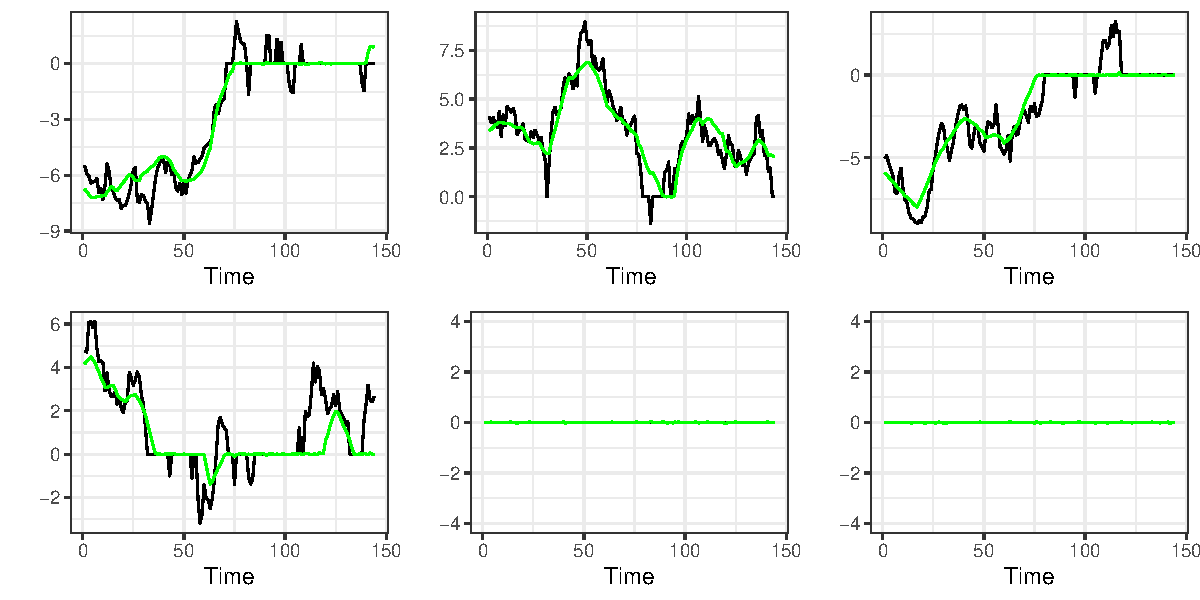
\includegraphics{Dynamic-Shrinkage-in-Bayesian-Structural-Time-Series-and-Vector-Autoregressive-Models_files/figure-latex/myfig8-1} 

}

\caption{Dynamic EMVS for BSTS model; true values of $\beta_{1:T, j}$, $j=1, \ldots, 6$, (black) and MAP trajectory (green) of the first six regression coefficients.}\label{fig:myfig8}
\end{figure}

In details, Table \ref{tab:mytab3} shows that a BSTS with trend and
seasonality without dynamic shrinkage (\(\Omega=1\)) is not able to
individuate the source of signal, therefore the estimates are biased and
definitely not reliable. On the other hand, both the Dynamic SSVS and
Dynamic EMVS performed well. We fix
\(\sigma^{2}_{\tau}=\sigma^{2}_{\mu}=\sigma^{2}_{\delta}=0.1\). We
acknowledge that the latter is a strong assumption, however we find it
to work well for the estimation of the time series structural
components. Figure \ref{fig:myfig14} shows smoothing estimates for the
seasonal, the trend and the regression components.

\begin{figure}[H]

{\centering 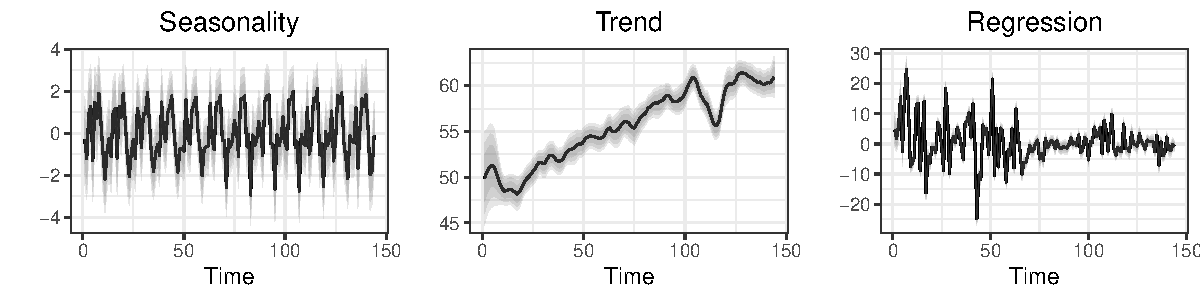
\includegraphics{Dynamic-Shrinkage-in-Bayesian-Structural-Time-Series-and-Vector-Autoregressive-Models_files/figure-latex/myfig14-1} 

}

\caption{Structural time series components. Point estimates (black) with credible intervals (gray).}\label{fig:myfig14}
\end{figure}

For the sake of completeness, the analysis is carried out for \(p=40\).
Results are promising and they are shown in the last rows of Table
\ref{tab:mytab3}. Overall, the Dynamic SSVS with \(\Omega=0.2\) shows
the best performance. In particular it is better than the Dynamic EMVS
in terms of SSE and Hamming distance. In addition, the simulation
algorithm did not produce any false detection or false non detection.

\begin{table}[H]

\caption{\label{tab:mytab3}Performance comparison}
\centering
\begin{tabular}[t]{ccccccccc}
\toprule
Dynamic & $\Omega$ & p & SSE & Ham. & FP & FN & FD & FND\\
\midrule
SSVS & 1 & 20 & 1796.832 & 2493 & 2493 & 0 & 16 & 0\\
SSVS & 0.2 & 20 & 569.214 & 106 & 44 & 62 & 0 & 0\\
EMVS & 0.2 & 20 & 590.676 & 149 & 85 & 64 & 3 & 0\\
SSVS & 0.2 & 40 & 610.903 & 113 & 44 & 69 & 0 & 0\\
EMVS & 0.2 & 40 & 702.192 & 190 & 114 & 76 & 8 & 0\\
\bottomrule
\end{tabular}
\end{table}

\section{Macroeconomic Data}\label{Macro2}

Given the encouraging results obtained with synthetic data, here we
provide an empirical macroeconomic application concerning unemployment
forecasting. The unemployment time series is usually characterized by
seasonal and trend-cycle components due to cyclical phenomena such as
seasonal work and long-run economic fluctuations. However, in some
specific circumstances, macroeconomic shocks may hit abruptly the series
causing unexpected deviations from its natural path. For these reasons,
unemployment forecasting represents a good exercise to test the strength
of our model in capturing all these features. Therefore, the objective
of this analysis is to fit the time series of unemployment rate not
transformed and not seasonally adjusted.\\
The BSTS model used in this exercise incorporates monthly seasonality, a
stochastic trend with time-varying slope, and a large set of predictors
whose role is to explain possible shocks. Predictors include: lagged
values of the dependent variable, interest rates, financial and
economics indicators, unemployment claims, and Google Trends data. The
sources of the data are the Federal Reserve Economic Data
(FRED)\footnote{url: https://fred.stlouisfed.org/}, Yahoo
Finance\footnote{url: https://it.finance.yahoo.com/} and Google
Trends\footnote{url: https://trends.google.com/}. The third one is a
less conventional data source. In a nutshell, Google Trends is a free
service provided by Google LLC which is meant to inform the user about
how frequently a given search term is entered into Google's research
engine. However, Google Trends provides only relative frequencies of the
data, such that a value equal to \(100\) identifies the highest
frequency of the searched term over a certain period, while the value
\(0\) indicates the lowest.\\
The predictors are divided into two classes according to their
frequency. For variables that present a monthly frequency we considered
the lagged values, while for those having a daily frequency we
considered the contemporaneous values. The list of predictors used in
this study is provided in Appendix. More formally, the observation
equation of the model here proposed is \begin{equation}
y_{t}=\mu_{t}+\tau_{t}+\boldsymbol{w}_{t}'\boldsymbol{\beta}_{1,t}+\boldsymbol{z}_{t-1}'\boldsymbol{\beta}_{2,t-1}+\epsilon_{t}
\end{equation} which is the same as for model (3.1) (\ref{eq:dssbsts1}),
but with
\(\boldsymbol{x}_{t}=(\boldsymbol{w}_{t},\boldsymbol{z}_{t-1})\) and
\(\boldsymbol{\beta}_{t}=(\boldsymbol{\beta}_{1,t},\boldsymbol{\beta}_{2,t-1})\).\\
The problem of forecasting using contemporaneous data is often referred
to as ``nowcasting.'' Such a term was originally coined in metereology
to indicate the prediction of the present or the very near future of an
economic or business indicator. What makes nowcasting appealing is the
fact that official statistics are usually published with a time lag,
whereas other type of data, such as financial data or web data, are
available at lower frequencies. For example,
\protect\hyperlink{ref-CV_2009}{Varian and Choi}
(\protect\hyperlink{ref-CV_2009}{2009b}) had the idea of using Google
Trends data for anticipating the release of official statistics.
Official statistics are indeed released one or even two weeks after the
end of the month while web data related to them are updated every day.
This allows to gather meaningful information about the statistics of
interest before the release. For example, observing Figure
\ref{fig:myfig17}, where the time series of unemployment rate is
presented together with some correlated Google searches, it would be
evident that a certain correlation exists among them. Indeed, Google
searches show a similar seasonality and synchronous spikes in proximity
of shocking events. For instance, searches for unemployment depression,
unemployment insurance and unemployment agencies drastically increased
at the beginning of pandemic crisis. And while the official statistic
for unemployment rate in April 2020 was released only on 8th May 2020 by
the US Bureau of Labor Statistics, Google Trends data were already
available in April. Therefore, we could say that these Google Trends
anticipated the observed peak in unemployment rate.

\begin{figure}[H]

{\centering 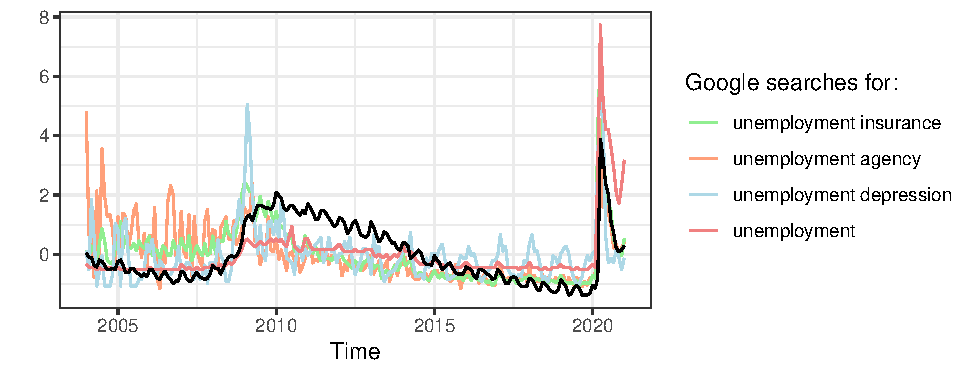
\includegraphics{Dynamic-Shrinkage-in-Bayesian-Structural-Time-Series-and-Vector-Autoregressive-Models_files/figure-latex/myfig17-1} 

}

\caption{Scaled time series of unemployment rate (black) and Google searches in different colors.}\label{fig:myfig17}
\end{figure}

Before proceeding to forecasting, we carry out a analysis we carry out
an explorative analysis. The hyperparameters are set in this way:
\(\Omega=0.2\), \(\phi_0=0\), \(\phi_1=0.98\), \(\lambda_0=0.01\) and
\(\lambda_1=0.1\). This setting prove good results in the
quasi-synthetic study and we maintain these choices here. After some
preliminary analysis performed with a large set of 61 predictors (40 of
which Google Trends), 12 seasonal factors, and a stochastic trend with a
time-varying slope we decide to manually select only 15 Google Trends
since we notice some redundancy in the information provided by some of
them. In particular, we remove the US states-specific ones, e.g.~``ny
unemployment'' and ``florida unemployment,'' and those not showing any
sort of correlation with the dependent variable. In addition, removing
collinear predictors allows for better identification and it reduces the
running time of the algorithms too.\\
As shown in Figure \ref{fig:myfig18}, the BSTS model succeed in
identifying the trend and seasonal components of the time series.
Instead, Google Trends data intervene principally in proximity of the
pandemic crisis, as reported also in Figure \ref{fig:myfig19} which
shows that six predictors are particularly important for anticipating
the event. The latter are: ``searches for unemployment,'' ``federal
unemployment,'' ``unemployment check,'' ``unemployment depression,''
``unemployment office'' and ``unemployment pa.''

\begin{figure}[H]

{\centering 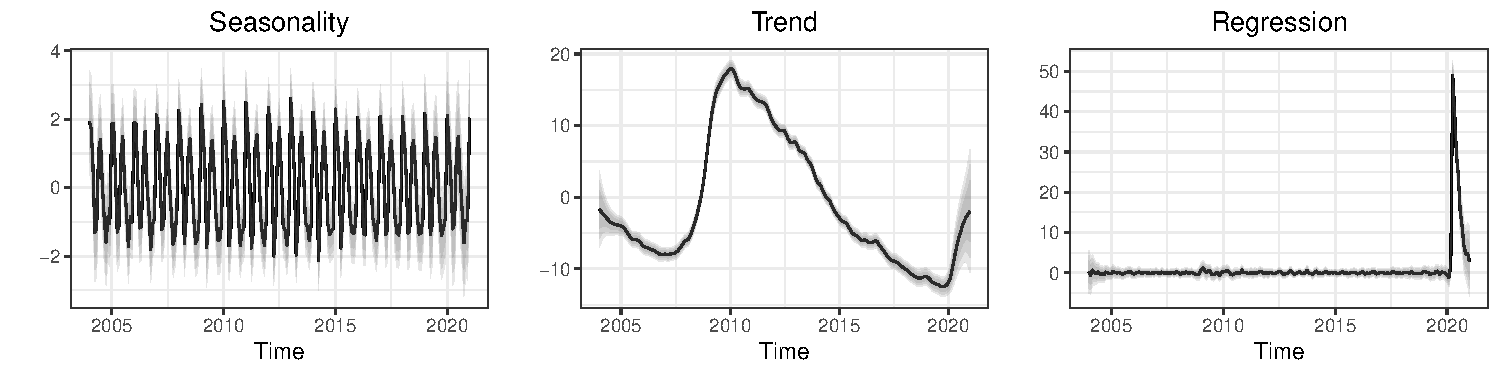
\includegraphics{Dynamic-Shrinkage-in-Bayesian-Structural-Time-Series-and-Vector-Autoregressive-Models_files/figure-latex/myfig18-1} 

}

\caption{Structural time series components. MCMC approximation of the expected values and their credible intervals. Data are rescaled to better visualize the main features.}\label{fig:myfig18}
\end{figure}

\begin{figure}[H]

{\centering 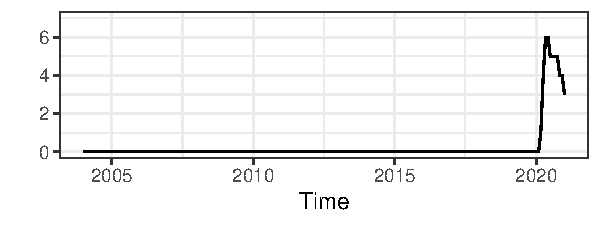
\includegraphics{Dynamic-Shrinkage-in-Bayesian-Structural-Time-Series-and-Vector-Autoregressive-Models_files/figure-latex/myfig19-1} 

}

\caption{Number of active TVP regression coefficients that contribute to unemployment rate nowcasting.}\label{fig:myfig19}
\end{figure}

We wondered why many Google Trends are insignificant and, in particular,
why some of them can anticipate the 2020 pandemic crises but none of
them can anticipate the 2008 financial crises. The answers we found are
the following. Firstly, Google economists used to rely on another and
maybe more powerful tool called Google Correlate. The difference between
the two services is that in Google Correlate the user uploaded a time
series and the system returned directly the most correlated queries. On
the other hand, in Google Trends correlated series have to be selected
manually. This makes it more difficult to include interesting predictors
inside the model. Secondly, Google Trends data can assume only discrete
values that depend on the time frame considered since they are rescaled
according to the rule mentioned before. This fact may explain why Google
Trends seem to have an important role in anticipating the pandemic
crisis while they are insignificant for predicting the financial crises
of 2008. We notice indeed that the enormous increase in Google searches
due to the pandemic flatten the series to zero at every other time.\\
Once we admit that there is a difference between the two crisis also
under the aspect of Google searches, then it is then natural to wonder
why this occurs. In our opinion, the huge increase in Google searches
during the pandemic crisis can be due to two possible causes. The
lockdown, which forced people to stay at home, and the recent
possibility to use web tools to search a job and carry out
administrative procedure such as unemployment benefits applications.
This can explain why the use of Google has been more intense during the
pandemic crisis compared to the financial crisis.\\
In any case, the model we developed is enough flexible to perform well
even in the absence of relevant predictors. This is shown in Figure
\ref{fig:myfig501} in which we compare the volatility process of two
BSTS models with dynamic shrinkage, one including all the predictors we
mentioned, i.e.~economic variables and Google Trends, and the other
including only one predictor, i.e.~the one period lag of the dependent
variable. In the first case (left panel) the model is able to capture
the predictable dependence through the (flexible) conditional mean. In
the second case (right panel), instead, the shock is captured by the
residuals' variance, which increase during the pandemic crisis.

\begin{figure}[h]

{\centering 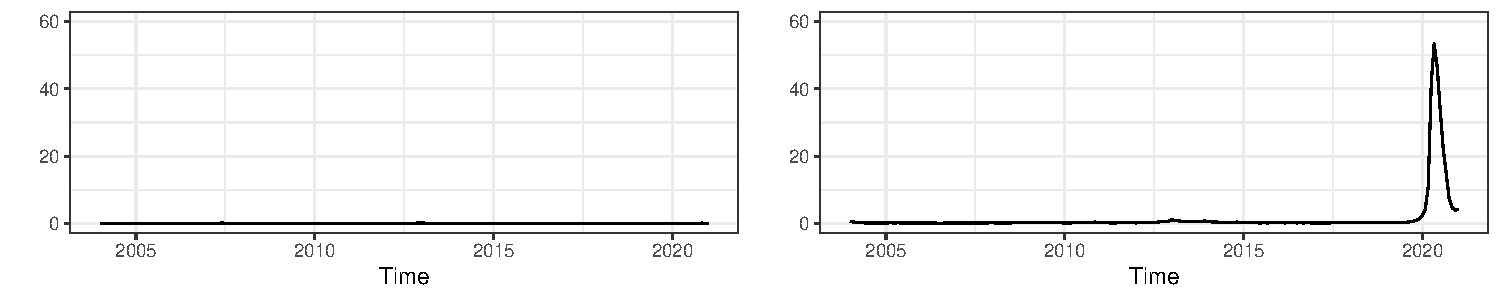
\includegraphics{Dynamic-Shrinkage-in-Bayesian-Structural-Time-Series-and-Vector-Autoregressive-Models_files/figure-latex/myfig501-1} 

}

\caption{Left panel: MCMC approximation of the expected values of $\sigma_{\epsilon,t}=\exp(h_t/2)$ of a BSTS model with 36 predictors, including economic indicators and Google Trends data. Right panel: MCMC approximation of the expected values of $\sigma_{\epsilon,t}=\exp(h_t/2)$ of a BSTS model with one predictors, i.e. the one period lag of unemployment rate.}\label{fig:myfig501}
\end{figure}

Let us focus on the forecasting performances. Because of the shock due
to the pandemic crisis, that induces structural changes, we decided to
split the time series in two periods: from 2004-01-01, day in which
Google Trends was released by Google Inc., to 2013-08-01 and from
2011-06-01 to 2020-12-01. The last 20 observations of each period form
the testing set. The idea is to evaluate the model's performances both
under standard conditions and when shocks occur. The objective is to
show that BSTS with dynamic shrinkage and stochastic volatility
represents a very flexible approach to time series modeling and
forecasting. In Tables \ref{tab:mytab31} and \ref{tab:mytab32},
forecasting performances of diverse specifications of Bayesian
Structural Time Series models are compared. Under standard conditions,
the model endowed with a seasonal component, which we call ``seasonal
model,'' provides better results. On the other hand, contrary to
expectations, the full (\(\Omega=1\)) non-seasonal model performs
curiously better than the shrunk (\(\Omega=0.2\)) non-seasonal model.
This effect is due to the seasonality shown by some predictors that may
help the model with more predictors to approximate somehow the seasonal
component of the dependent variable. Note, however, that seasonal
fluctuations observed in the explanatory variables are usually caused by
weather effects, administrative measures or other events that may not
affect significantly the dependent variable. This explains the better
accuracy obtained using a seasonal component rather than extracting the
seasonality from the predictors. On the other hand, regarding the
quantification of the uncertainty, the similar SLPL between the models
with and without seasonality when \(\Omega=1\) (as shown in Table
\ref{tab:mytab31}) can be explained by the larger credible intervals due
to the bigger size of the state vector in the seasonal model which tends
to inflate the state variance and, consequently, the forecast
variance.\\
On the other hand, by seasonally adjusting the predictors the resulting
picture becomes much more consistent with the expectations. Indeed
non-seasonal models are now completely unable to capture seasonal
fluctuations. The adjustment of the series has been carried out using
the X-13ARIMA-SEATS Seasonal Adjustment strategy of the Census Bureau.\\
So far we explained why a seasonal model should be preferred over a
non-seasonal one. Regarding the comparison dynamic shrinkage versus no
shrinkage, the results of this forecasting exercise are the following.
Even though the predictive means are rather similar in both models, the
reduction of the noise induced by shrinkage priors translates to
narrower credible intervals and hence into an higher reliability of the
point estimates. This peculiarity makes the penalized model preferable
under standard conditions. On the other hand, when big shocks occur, the
larger credible intervals produced by the full model allow to cover most
of the fluctuation observed in the time series of unemployment rate,
whereas the penalized model seems unable to properly represent the
uncertainty around the point forecasts. This happens because the
conditional inclusion probabilities evolve smoothly over time and they
are not adequate for sudden changes. Therefore, under regular
conditions, BSTS models with dynamic shrinkage are very promising for
time series analysis of high-dimensional non-stationary and not
seasonally adjusted time series. In order to make them more suitable
also for predicting shocking events, \(\Omega\) could be modeled as a
random variable with support \((0,1]\), whose hyperparameters are set as
a function of \(\sigma^{2}_{\epsilon,t}\). Developments in this
direction are not dealt with here.

\begin{table}[H]

\caption{\label{tab:mytab31}Not seasonally adjusted predictors}
\centering
\fontsize{8}{10}\selectfont
\begin{tabular}[t]{>{}ccccccccccc}
\toprule
\multicolumn{3}{c}{ } & \multicolumn{4}{c}{From 01/12/2011 to 01/08/2013} & \multicolumn{4}{c}{From 01/04/2019 to 01/12/2020} \\
\cmidrule(l{3pt}r{3pt}){4-7} \cmidrule(l{3pt}r{3pt}){8-11}
Dynamic & Seasonality & $\Omega$ & RMSE & WMAPE & MASE & SLPL & RMSE & WMAPE & MASE & SLPL\\
\midrule
 & Yes & 0.2 & 0.991 & 0.103 & 0.483 & -31.666 & 12.024 & 0.355 & 0.957 & -132.723\\
\cmidrule{2-11}
 & Yes & 1 & 0.905 & 0.096 & 0.45 & -40.387 & 10.428 & 0.325 & 0.875 & -58.027\\
\cmidrule{2-11}
 &  & 0.2 & 2.095 & 0.207 & 0.973 & -82.824 & 11.232 & 0.383 & 1.032 & -121.247\\
\cmidrule{2-11}
\multirow[t]{-4}{*}{\centering\arraybackslash SSVS} &  & 1 & 1.772 & 0.17 & 0.795 & -41.912 & 10.53 & 0.333 & 0.898 & -56.185\\
\cmidrule{1-11}
 & Yes & 0.2 & 1.312 & 0.141 & 0.602 & - & 8.365 & 0.352 & 0.949 & -\\
\cmidrule{2-11}
 & Yes & 1 & 1.36 & 0.137 & 0.585 & - & 8.422 & 0.362 & 0.977 & -\\
\cmidrule{2-11}
 &  & 0.2 & 1.8 & 0.181 & 0.847 & - & 9.61 & 0.373 & 1.006 & -\\
\cmidrule{2-11}
\multirow[t]{-4}{*}{\centering\arraybackslash EMVS} &  & 1 & 1.807 & 0.165 & 0.776 & - & 9.231 & 0.368 & 0.992 & -\\
\bottomrule
\end{tabular}
\end{table}

\begin{table}[H]

\caption{\label{tab:mytab32}Seasonally adjusted predictors}
\centering
\fontsize{8}{10}\selectfont
\begin{tabular}[t]{>{}ccccccccccc}
\toprule
\multicolumn{3}{c}{ } & \multicolumn{4}{c}{From 01/12/2011 to 01/08/2013} & \multicolumn{4}{c}{From 01/04/2019 to 01/12/2020} \\
\cmidrule(l{3pt}r{3pt}){4-7} \cmidrule(l{3pt}r{3pt}){8-11}
Dynamic & Seasonality & $\Omega$ & RMSE & WMAPE & MASE & SLPL & RMSE & WMAPE & MASE & SLPL\\
\midrule
 & Yes & 0.2 & 1.019 & 0.107 & 0.504 & -31.389 & 11.448 & 0.298 & 0.804 & -174.256\\
\cmidrule{2-11}
 & Yes & 1 & 0.943 & 0.093 & 0.437 & -39.315 & 10.541 & 0.293 & 0.791 & -61.855\\
\cmidrule{2-11}
 &  & 0.2 & 2.083 & 0.212 & 0.994 & -46.198 & 13.502 & 0.514 & 1.386 & -116.424\\
\cmidrule{2-11}
\multirow[t]{-4}{*}{\centering\arraybackslash SSVS} &  & 1 & 2.267 & 0.232 & 1.091 & -50.392 & 9.901 & 0.32 & 0.864 & -60.674\\
\cmidrule{1-11}
 & Yes & 0.2 & 1.042 & 0.148 & 0.628 & - & 10.693 & 0.305 & 0.822 & -\\
\cmidrule{2-11}
 & Yes & 1 & 1.042 & 0.16 & 0.683 & - & 9.796 & 0.301 & 0.812 & -\\
\cmidrule{2-11}
 &  & 0.2 & 2.076 & 0.198 & 0.931 & - & 12.781 & 0.429 & 1.158 & -\\
\cmidrule{2-11}
\multirow[t]{-4}{*}{\centering\arraybackslash EMVS} &  & 1 & 2.258 & 0.23 & 1.078 & - & 13.17 & 0.437 & 1.179 & -\\
\bottomrule
\end{tabular}
\end{table}

\begin{figure}[H]

{\centering 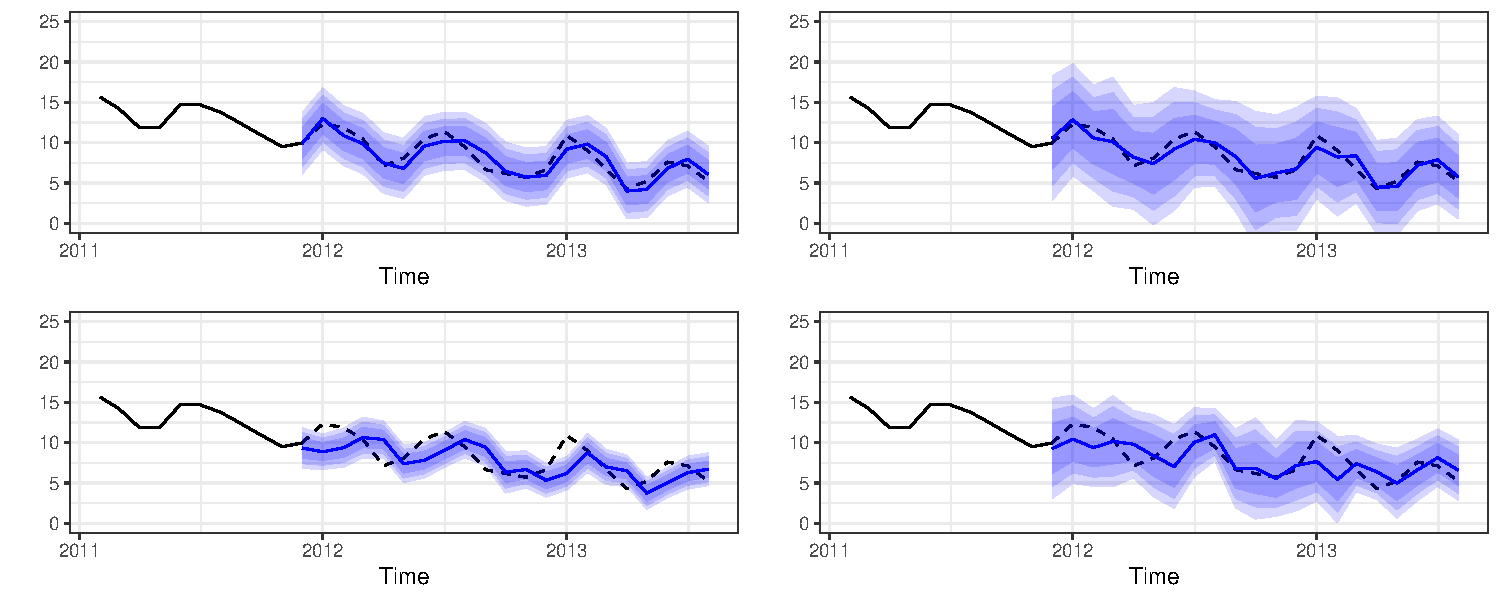
\includegraphics{Dynamic-Shrinkage-in-Bayesian-Structural-Time-Series-and-Vector-Autoregressive-Models_files/figure-latex/myfig117-1} 

}

\caption{Not seasonally adjusted predictors. One-step-ahead forecasts (blue) with their credible intervals and the true series (black). Upper-left panel: Seasonal BSTS model with $\Omega=0.2$. Bottom-left panel: Not seasonal BSTS model with $\Omega=0.2$. Upper-right panel: Seasonal BSTS model with $\Omega=1$. Bottom-right panel: Not seasonal BSTS model with $\Omega=1$. These plots shows how the model behaviour under regular conditions.}\label{fig:myfig117}
\end{figure}

\begin{figure}[H]

{\centering 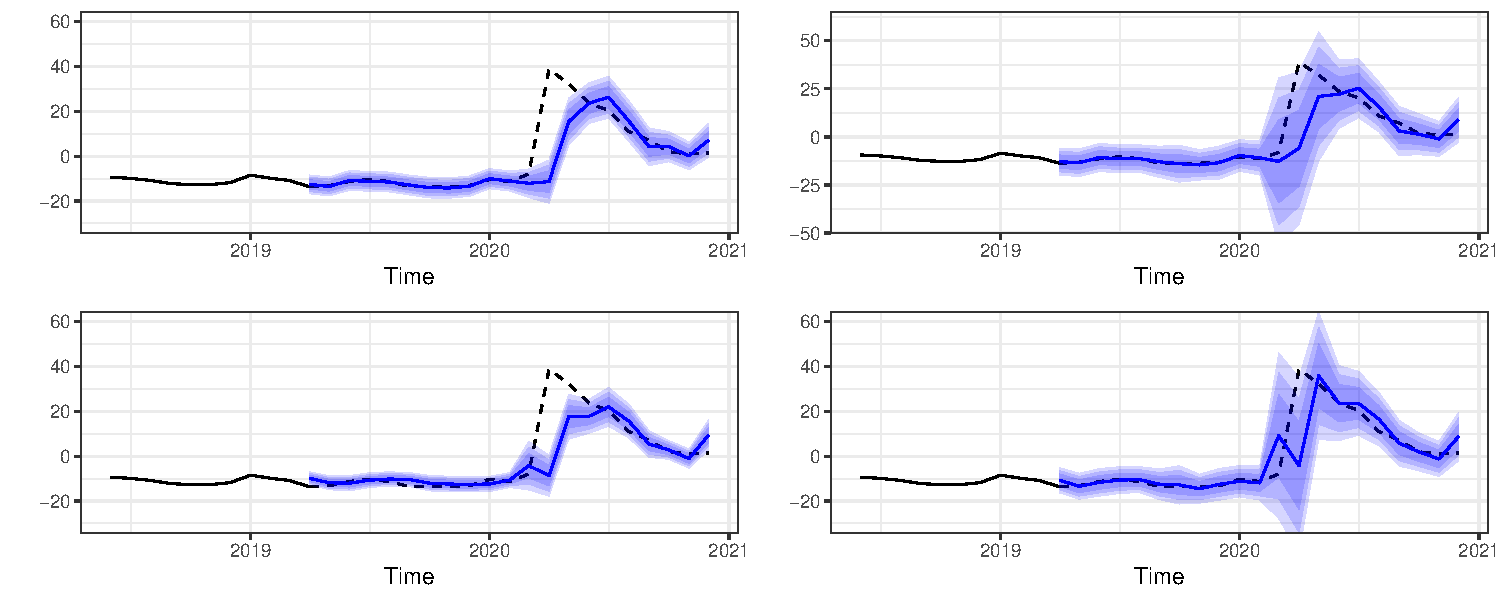
\includegraphics{Dynamic-Shrinkage-in-Bayesian-Structural-Time-Series-and-Vector-Autoregressive-Models_files/figure-latex/myfig118-1} 

}

\caption{Not seasonally adjusted predictors. One-step-ahead forecasts (blue) with their credible intervals and the true series (black). Upper-left panel: Seasonal BSTS model with $\Omega=0.2$. Bottom-left panel: Not seasonal BSTS model with $\Omega=0.2$. Upper-right panel: Seasonal BSTS model with $\Omega=1$. Bottom-right panel: Not seasonal BSTS model with $\Omega=1$. These plots shows how the model behaviour when shocks occur.}\label{fig:myfig118}
\end{figure}

\begin{figure}[H]

{\centering 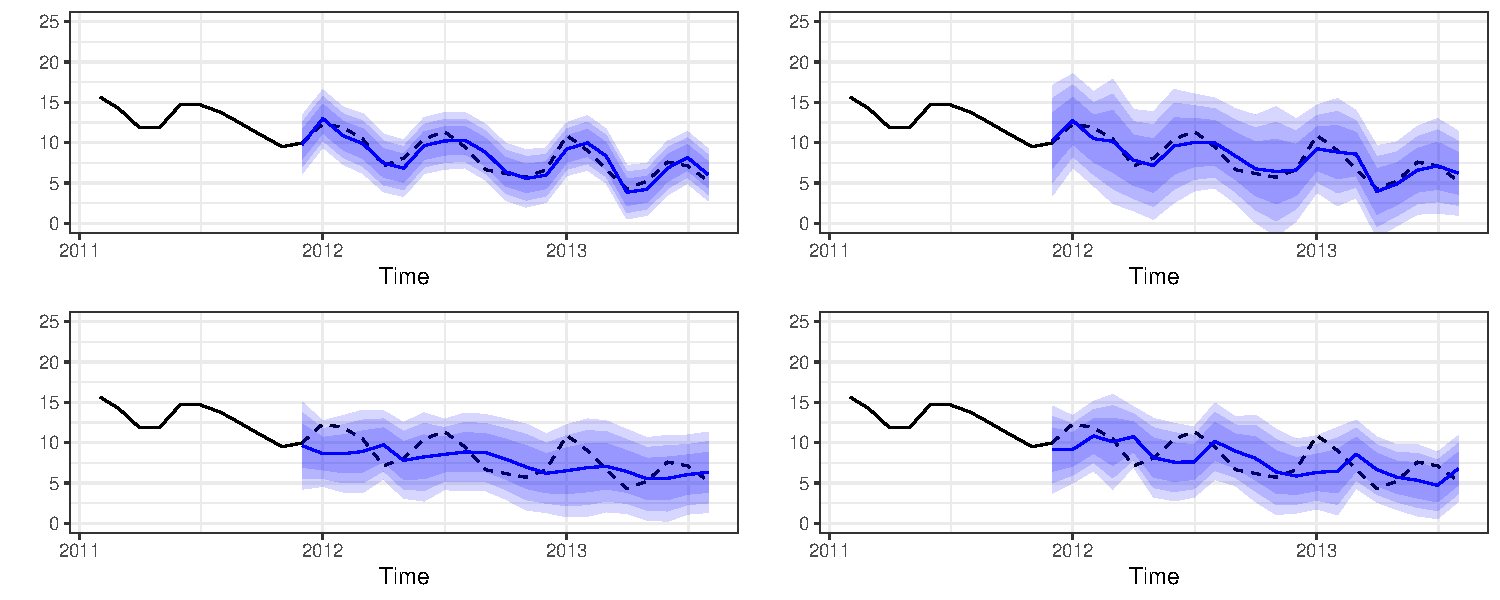
\includegraphics{Dynamic-Shrinkage-in-Bayesian-Structural-Time-Series-and-Vector-Autoregressive-Models_files/figure-latex/myfig119-1} 

}

\caption{Seasonally adjusted predictors. One-step-ahead forecasts (blue) with their credible intervals and the true series (black). Upper-left panel: Seasonal BSTS model with $\Omega=0.2$. Bottom-left panel: Not seasonal BSTS model with $\Omega=0.2$. Upper-right panel: Seasonal BSTS model with $\Omega=1$. Bottom-right panel: Not seasonal BSTS model with $\Omega=1$. These plots shows how the model behaviour under regular conditions.}\label{fig:myfig119}
\end{figure}

\begin{figure}[H]

{\centering 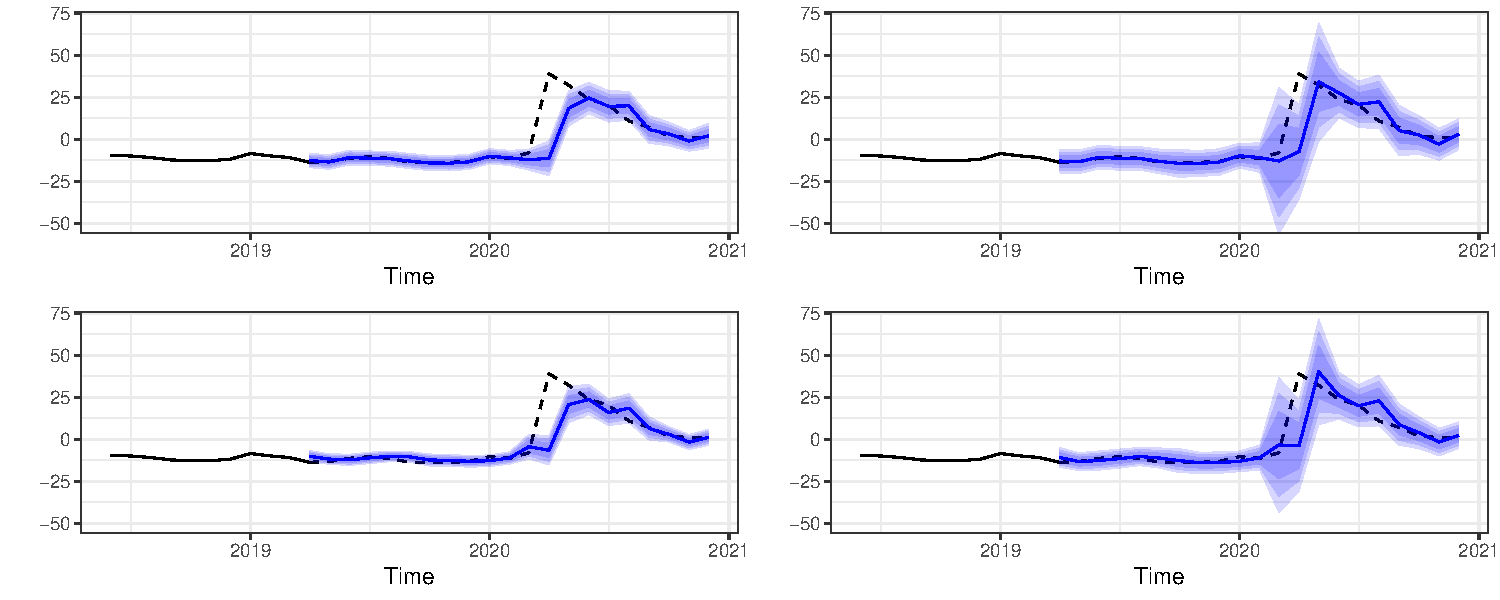
\includegraphics{Dynamic-Shrinkage-in-Bayesian-Structural-Time-Series-and-Vector-Autoregressive-Models_files/figure-latex/myfig120-1} 

}

\caption{Seasonally adjusted predictors. One-step-ahead forecasts (blue) with their credible intervals and the true series (black). Upper-left panel: Seasonal BSTS model with $\Omega=0.2$. Bottom-left panel: Not seasonal BSTS model with $\Omega=0.2$. Upper-right panel: Seasonal BSTS model with $\Omega=1$. Bottom-right panel: Not seasonal BSTS model with $\Omega=1$. These plots shows how the model behaviour when shocks occur.}\label{fig:myfig120}
\end{figure}

\section{Discussion}

Bayesian Structural Time Series models with Dynamic Spike-and-Slab
regression and stochastic volatility represent the natural evolution of
the model proposed by \protect\hyperlink{ref-scott_varian_2013}{Scott
and Varian} (\protect\hyperlink{ref-scott_varian_2013}{2013}). For the
same reasons we allow for stochastic fluctuations in the trend, slope,
and seasonality, it is logical to model the remaining parameters as
time-varying too. The assumption of constant regression coefficients may
hold when it found justification on physical models or when the time
series evolves over few years. On the other hand, this assumption is
likely to be too limiting for most applications, particularly in the
economic and social sciences. The analysis presented in the preceding
paragraph demonstrates this fact by proving that some predictors, in
that case Google Trends data, play an important role when the time
series exhibits shocks that cause it to deviate from its natural
pattern. Otherwise, the time series can be satisfactorily modeled using
a simple BSTS model with trend and seasonality. This raise two
considerations. To begin with, simple models can occasionally operate
admirably. In this scenario, adding predictors is not only pointless,
but it also diminishes the model's interpretability, which is critical
for economists. As a result, our novel class of BSTS models fits for the
purpose since it is particularly parsimony oriented, permitting the
intervention of additional predictors only when absolutely essential.
Second, while time-varying coefficients can capture both permanent and
transient phenomena like the pandemic crisis, time-varying residual
variances hedge the researcher against biases that may arise as a
consequence of the exclusion of some important predictors. The model
indeed would still work without the need to adjust parameter estimates
also in the latter case. Overall, the results obtained using both
simulated and real data are consistent with our goal of developing a
highly flexible model that can be used to analyze long macroeconomic
time series under a variety of scenarios. On the other hand, the
analysis brings out some limitations of our approach too. The most
crucial ones have concern how to deal with the model's hyperparameters.
In particular, \(\Omega\), which drives shrinkage globally, may be
recalibrated in proximity of structural breaks. This would make the
model even more flexible. Therefore, further developments on this issue
will follow. A possible solution we envisage is to consider \(\Omega\)
as a random variable and letting its values changing according to the
magnitude of shocking events such as the one exhibited by the
unemployment rate in April 2020.

\chapter[Multivariate Time Series Models]{Dynamic Shrinkage in Multivariate Time Series Models}\label{Dynamic Shrinkage in Multivariate Time Series Models}

Introducing dynamic shrinkage methods in multivariate time series models
is undoubtedly interesting and challenging at the same time.
Multivariate time series models are widely used and they are often
necessary to study macroeconomic phenomena phenomena, that are
characterized by the interactions of many economic variables so that
univariate models can hardly capture all the dynamics of interest. A
multivariate model allows to better describe past and contemporaneous
relationships between the key variables. This however comes with some
costs. When the number of dependent variables increases, the curse of
dimensionality becomes more severe and it may eventually be
unsustainable. For this reason, many authors have addressed their
researches to the development of variable selection methods in this
area. Nevertheless, dynamic shrinkage in multivariate time series
analysis is still an open problem. With this chapter we want to provide
a small contribution in this direction by embedding the Dynamic
Spike-and-Slab process priors within the framework of Time-Varying
Parameter Vector Autoregressive (TVP-VAR) models.

\section{Time-Varying Parameter VAR Models}

The introduction of TVP-VAR models into the literature was prompted by a
wide range of phenomena observed in time series analysis between the
1960s and the 1990s. For instance, strong evidence suggests that
unemployment and inflation in the United States were greater and more
volatile in the 1960s and 1970s than in the 1980s and 1990s. Such
changes in the model parameters are difficult to be modeled within the
classical frequentist framework of VAR models and this encouraged
researcher to adopt a Bayesian approach. In the last decades, many
authors developed even more flexible and sophisticated models in which
the regression parameters or the residual variances are subject to
stochastic variations. Some interesting contributions in this direction
come from \protect\hyperlink{ref-CANOVA_1993}{Canova and Dellas}
(\protect\hyperlink{ref-CANOVA_1993}{1993}),
\protect\hyperlink{ref-CS_2001}{Stock}
(\protect\hyperlink{ref-CS_2001}{2001}) and
\protect\hyperlink{ref-COGLEY2005262}{Cogley and Sargent}
(\protect\hyperlink{ref-COGLEY2005262}{2005}), to mention a few.\\
The assumption of time-varying parameters should be natural. For example
recent structural macroeconomic shocks such as the 2008 financial crisis
and the pandemic crisis, would suggest time varying models, that are
likely to become the standard in macroeconomics. However, the lack of a
variable selection mechanism in these models has limited their potential
for many interesting applications. This limitation has however
stimulated a growing research in this topic. Here we decided to focus on
the Time-Varying Parameter VAR model of
\protect\hyperlink{ref-Primicieri_2005}{Primiceri}
(\protect\hyperlink{ref-Primicieri_2005}{2005}) that had a certain
impact in the econometric literature. Our contribution is to extend this
model by allowing for dynamic variable selection through a Dynamic
Spike-and-Slab Process Priors. With respect to previous approaches which
focused on heteroschedasticity or time-varying regression coefficients,
the model of \protect\hyperlink{ref-Primicieri_2005}{Primiceri}
(\protect\hyperlink{ref-Primicieri_2005}{2005}) includes both of them.
This model is particularly flexible since it provides a data-driven
guidance in establishing whether the overall time variation of the
linear structure is explained by a change in the size of the shocks, and
hence in the volatility process, or a change in the propagation
mechanism, and hence the coefficients. Formally, let
\(\boldsymbol{y}_{t}\) be an \(n \times 1\) vector of observations, for
\(t=1,...,T\), the TVP-VAR is \begin{equation}\label{eq:TVPVAR1}
\boldsymbol{y}_{t}=\boldsymbol{c}_{t}+\sum_{h=1}^{H}\boldsymbol{B}_{h,t}\boldsymbol{y}_{t-h}+\boldsymbol{\epsilon}_{t}, \ \ \ \boldsymbol{\epsilon}_{t}\sim\mathcal{N}(\boldsymbol{0},\Omega_{t})
\end{equation} where \(\boldsymbol{c}_{t}\) is a \(n \times 1\) vector
of time-varying coefficients associated to a constant term,
\(\boldsymbol{B}_{h,t}\) (for \(h=1,...,H\) number of lags) is a
\(n \times n\) matrix of time varying coefficients and \(\epsilon_{t}\)
is a vector of \(n \times 1\) residuals. For identificability reasons we
follow the proposal of \protect\hyperlink{ref-SIMS_1980}{Sims}
(\protect\hyperlink{ref-SIMS_1980}{1980}) and we assume a lower
triangular matrix \(\boldsymbol{A}_{t}\) of contemporaneous relationship
such that \begin{equation*}
\boldsymbol{A}_{t}\Omega_{t}\boldsymbol{A}_{t}'=\Sigma_{t}^{\frac{1}{2}}\Sigma_{t}'^{\frac{1}{2}}
\end{equation*} and \[ \boldsymbol A_{t} = \begin{pmatrix}
  1 & 0 & ... & 0 \\
  \alpha_{2 1,t} & 1 & ... & 0 \\
  \vdots  & \vdots  & \ddots & \vdots \\
  \alpha_{n1,t} & ... & \alpha_{n n-1,t} & 1
  \end{pmatrix}\] while \[ \Sigma_{t} = \begin{pmatrix}
  \sigma^{2}_{1,t} & 0 & ... & 0 \\
  0 & \sigma^{2}_{2,t} & ... & 0 \\
  \vdots  & \vdots  & \ddots & \vdots \\
  0 & ... & 0 & \sigma^{2}_{n,t}
  \end{pmatrix}\] A more convenient way to write equation
(\ref{eq:TVPVAR1}) is \begin{equation*}
\boldsymbol{y}_{t}=\boldsymbol{c}_{t}+\sum_{h=1}^{H}\boldsymbol{B}_{h,t}\boldsymbol{y}_{t-h}+\boldsymbol{A}^{-1}_{t}\Sigma_{t}^{\frac{1}{2}}\boldsymbol{\epsilon}_{t}, \ \ \ \boldsymbol{\epsilon}_{t}\sim\mathcal{N}(\boldsymbol{0},\boldsymbol{I}_{n})
\end{equation*} This equation can be re-written more compactly in state
space form. Let
\(\boldsymbol{X}'_{t}\equiv\boldsymbol{I}_{n}\otimes (1,\boldsymbol{y}_{t-1}',...,\boldsymbol{y}_{t-H}')\)
and
\(\boldsymbol{\beta}_{t}\equiv vec([\boldsymbol{c}_t,\boldsymbol{B}_{1,t},...,\boldsymbol{B}_{H,t}]')\),
then \begin{equation}\label{eq:ssmtvp}
\boldsymbol{y}_{t}=\boldsymbol{X}_{t}'\boldsymbol{\beta}_{t}+\boldsymbol{A}_{t}^{-1}\Sigma_{t}^{\frac{1}{2}}\boldsymbol{\epsilon}_{t}, \ \ \ \boldsymbol{\epsilon}\sim\mathcal{N}(\boldsymbol{0},\boldsymbol{I}_{n})
\end{equation} \protect\hyperlink{ref-Primicieri_2005}{Primiceri}
(\protect\hyperlink{ref-Primicieri_2005}{2005}) considers the regression
coefficients \(\boldsymbol{\beta}_{t}\), the elements \(\alpha_{ij,t}\)
of the matrix \(\boldsymbol{A}_{t}\), and the logarithm of the diagonal
elements of \(\Sigma_{t}\) to behave like random walks. Even though this
specification has the advantage of reducing the number of unknown
parameters which is already large, it also entails undesirable
implications from a theoretical point of view since random walk
processes are intrinsically unstable. Moreover, although
\protect\hyperlink{ref-rockova_mcalinn_2021}{Rockova and McAlinn}
(\protect\hyperlink{ref-rockova_mcalinn_2021}{2021a}) observe that it
would be possible to extend the DSS approach to a random walk slab
process by reformulating opportunely the transition weights, one must be
careful to avoid the series \(\omega_{1:T}\) being too unstable. This
would indeed lead to erratic transitions from the spike to slab and vice
versa. Therefore, we will stick to the considerations made in Chapter
\ref{Dynamic Shrinkage} and assume the regression coefficients to follow
independent stationary Gaussian AR(1) processes. The dynamics of the
model is described by the following equations: \begin{equation}
\begin{aligned}\label{EQ:dmodel}
\boldsymbol{y}_{t} = & \boldsymbol{X}_{t}'\boldsymbol{\beta}_{t}+\boldsymbol{A}_{t}\Sigma^{\frac{1}{2}} \boldsymbol{\epsilon}_{t},\\
\boldsymbol{\beta}_{t} = & \boldsymbol{G}_{t}^{(\beta)}\boldsymbol{\beta}_{t-1}+\boldsymbol{\xi}_{t},\\
\boldsymbol{\alpha}_{t} = & \boldsymbol{G}_{t}^{(\alpha)}\boldsymbol{\alpha}_{t-1}+\boldsymbol{\eta}_{t},\\
\boldsymbol{h}_{t} = & \boldsymbol{\mu} + \boldsymbol{R}(\boldsymbol{h}_{t-1}-\boldsymbol{\mu})+\boldsymbol{\zeta}_{t}
\end{aligned}
\end{equation} where
\(\boldsymbol{G}_{t}^{(\beta)}=diag\{\gamma_{t,j}^{(\beta)}\phi_{1}\}_{j=1}^{p_\beta}\),
\(\boldsymbol{G}_{t}^{(\alpha)}=diag\{\gamma_{t,j}^{(\alpha)}\phi_{1}\}_{j=1}^{p_\alpha}\),
\(\boldsymbol{\mu}=(\mu_{1},...,\mu_{n})'\) and
\(\boldsymbol{R}=diag(\rho_1,...,\rho_n)\). The parameter \(\phi_1\)
will be set equal to 0.98 in the applications that will follow. We
acknowledge that such assumption may seem too strong, however empirical
analysis proved that fixing \(\phi_1\) close to one leads to satisfying
results while preserving stationary. On the other hand, it would be
possible to assign a Beta distribution to this parameter and update its
posterior; however, this would inevitably increase the amount of unknown
parameters and add further steps into the MCMC scheme with the
consequent increase in the running time (which is already long).
Regarding the choice of \(\boldsymbol{\beta}_{0}\) and
\(\boldsymbol{\alpha}_{0}\), one may assume a Gaussian distribution
centered on the least squares estimates computed on a subsample of the
data or on the whole sample with large variance. Alternatively, another
strategy is to model
\(\boldsymbol{\beta}_{0}\sim\mathcal{N}(\boldsymbol{m}_0,\boldsymbol{C}_0)\)
where \(\boldsymbol{m}_0=\phi_1\boldsymbol{\gamma}_{0}^{(\beta)}\) and
\(\boldsymbol{C}_0=diag\{\gamma_{0,j}^{(\beta)}\lambda_1/(1+\phi_1)+(1-\gamma_{0,j}^{(\beta)})\lambda_0\}_{j=1}^{p_\beta}\)
and same for \(\boldsymbol{\alpha}_0\).\\
In this model we distinguish between two types of auxiliary variables:
\(\gamma_{t,j}^{(\beta)}\) and \(\gamma_{t,j}^{(\alpha)}\). The reason
behind this separation is that we consider relationships between
contemporaneous variables more meaningful with respect to the ones with
lagged values of the variables. Therefore we would set
\(\Omega_{\alpha}\) close to one and \(\Omega_\beta\) commensurate to
the number of lags of our model such that models with more lags are
shrunk with greater severity. Our proposal is to assume that both
\(\beta_{1:T,j}\) and \(\alpha_{1:T,k}\) for \(j=1,...,p_\beta\) and
\(k=1,...,p_\alpha\) are i.i.d. distributed with DSS priors. That is, we
assume that the generic \(\beta_t\) has a mixture density prior of the
kind \begin{equation*}
\pi(\beta_{t}|\gamma_{t},\beta_{t-1})=(1-\gamma_{t})\psi_{0}(\beta_{t}|\lambda_{0})+\gamma_{t}\psi_{1}(\beta_{t}|\mu_{t},\lambda_{1})
\end{equation*} where \begin{equation*}
\mu_{t}=\phi_{0}+\phi_{1}(\beta_{t-1}-\phi_{0}) \ \ \ \text{with} \ \ \ |\phi_{1}|<1
\end{equation*} and \begin{equation*}
P(\gamma_{t}=1|\beta_{t-1})=\omega_{t}^{(\beta)}
\end{equation*} The inclusion probabilities \(\omega_{t}^{(\beta)}\) are
definite exactly as in Chapter \ref{Dynamic Shrinkage} and they depend
on \(\Omega_\beta\). Analogously we assign DSS priors on \(\alpha_t\).
Finally, we assume that \[ 
( \boldsymbol{\xi}_{t}, \boldsymbol{\eta}_{t}, \boldsymbol{\zeta}_{t})' \sim \mathcal{N}(\boldsymbol{0},\boldsymbol{W}_{t})
\] where \[ \boldsymbol{W}_{t} = \begin{pmatrix}
  \Lambda_{\beta} & 0 &  0 \\
  0 & \Lambda_{\alpha} & 0 \\
  0 & 0 & \Sigma_{\zeta} 
  \end{pmatrix}\] with
\(\Lambda_{\beta}=\{\gamma_{t,j}^{(\beta)}\lambda_{1}+(1-\gamma_{t,j}^{(\beta)})\lambda_0\}_{j=1}^{p_{\beta}}\),
\(\Lambda_{\alpha}=\{\gamma_{t,j}^{(\alpha)}\lambda_{1}+(1-\gamma_{t,j}^{(\alpha)})\lambda_0\}_{j=1}^{p_{\alpha}}\)
and
\(\Sigma_{\zeta}=diag(\sigma^{2}_{\zeta,1},...,\sigma^{2}_{\zeta,n})\).
The hyperparameters \(\lambda_1\) and \(\lambda_0\) must be fixed in
such a way that allows a sufficiently large ratio between spike and slab
variances (\protect\hyperlink{ref-GM_1993}{George and McCulloch 1993}).
For example, in the empirical study of Section \ref{MD3}, we notice that
fixing \(\lambda_1=0.1\) and \(\lambda_0=0.01\) provides satisfying
results. In general, we recommend to repeat the study for different
values of \(\lambda_0\) and \(\lambda_1\) and pick the ones that produce
the best predictive performances. The parameters
\(\sigma_{\zeta,i}^{2}\) for \(i=1,...,n\) are independently estimated
using the sampling strategy described in Section
\ref{A new proposal for the volatility process}.

\subsection{Dynamic Stochastic Search Variable Selection}

Efficient posterior sampling for the TVP-VAR model with dynamic
shrinkage can be performed using a Dynamic SSVS strategy. A possible
sampling scheme is the one proposed by
\protect\hyperlink{ref-Primicieri_2005}{Primiceri}
(\protect\hyperlink{ref-Primicieri_2005}{2005}) that we extend in order
to deal with the dynamic shrinkage components, as reported below. The
overall strategy, resumed in Algorithm \ref{alg:dstvpvar}. We here
detail the main steps. Let
\(\boldsymbol{\gamma}=(\boldsymbol{\gamma}^{(\beta)},\boldsymbol{\gamma}^{(\alpha)})\)
then

\begingroup
\LinesNumbered
\begin{algorithm}[t]
\caption{Dynamic Shrinkage in Time-Varying Parameter VAR models} \label{alg:dstvpvar}
 Draw $\boldsymbol{\beta}$ from $\pi(\boldsymbol{\beta}|\boldsymbol{y},\boldsymbol{\Sigma},\boldsymbol{A},\boldsymbol{\gamma},\boldsymbol{W})$ \;
 Draw $\boldsymbol{A}$ from $\pi(\boldsymbol{A}|\boldsymbol{y},\boldsymbol{\beta},\boldsymbol{\gamma},\boldsymbol{\Sigma},\boldsymbol{W})$ \;
 Draw $\gamma_{j,t}^{(\beta)}$ individually and independently from $\pi(\gamma_{j,t}^{(\beta)}|\boldsymbol{y},\boldsymbol{\beta},\boldsymbol{A},\boldsymbol{\Sigma},\boldsymbol{W},\boldsymbol{\gamma}_{-j,t}^{(\beta)})$ and $\gamma_{j,t}^{(\alpha)}$ individually and independently from $\pi(\gamma_{j,t}^{(\alpha)}|\boldsymbol{y},\boldsymbol{\beta},\boldsymbol{A},\boldsymbol{\Sigma},\boldsymbol{W},\boldsymbol{\gamma}_{-j,t}^{(\alpha)})$ \;
 Compute $\Lambda_{\beta}$ and $\Lambda_{\alpha}$\;
 Draw $\boldsymbol{\Sigma}$ from $\pi(\boldsymbol{\Sigma}|\boldsymbol{y},\boldsymbol{\beta},\boldsymbol{A},\boldsymbol{\gamma},\boldsymbol{W},\boldsymbol{\mu},\boldsymbol{R},\Sigma_{\zeta})$ \;
 Draw $\boldsymbol{\mu},\boldsymbol{R},\Sigma_{\zeta}$ independently from each time series using the passages illustrated in section \ref{A new proposal for the volatility process} \;
\end{algorithm}

\begin{itemize}
\item Step 1; Conditionally on $(\boldsymbol{y},\boldsymbol{\Sigma},\boldsymbol{A},\boldsymbol{\gamma},\boldsymbol{W})$, the space state model is linear and Gaussian with known variance, therefore draws from $\pi(\boldsymbol{\beta}|\boldsymbol{y},\boldsymbol{\Sigma},\boldsymbol{A},\boldsymbol{\gamma},\boldsymbol{W})$ can be obtained through FFBS algorithm.
\item Step 2; Let $\boldsymbol{y}_{t}-\boldsymbol{X}_{t}'\boldsymbol{\beta}_{t}=\hat{\boldsymbol{y}}_{t}$, which is observable once $\boldsymbol{\beta}_{t}$ is sampled, and note that equation (\ref{eq:ssmtvp}) can be rewritten as
\begin{equation}\label{eq:A1}
\boldsymbol{A}_{t}\hat{\boldsymbol{y}}_{t}=\Sigma^{\frac{1}{2}}_{t}\boldsymbol{\epsilon}_{t}
\end{equation}
Given the lower triangular shape of $\boldsymbol{A}_{t}$ with ones on its diagonal, then equation (\ref{eq:A1}) can be seen as a State-Space Model
\begin{equation}
\hat{\boldsymbol{y}}_{t}=\boldsymbol{Z}_{t}\boldsymbol{\alpha}_{t}+\Sigma^{\frac{1}{2}}_{t}\boldsymbol{\epsilon}_{t}
\end{equation}
where 
\[
\boldsymbol{Z}_{t} = \begin{pmatrix}
  0 & ... &  ... & 0 \\
  -\hat{y}_{1,t} & 0 & ... \\
  0 & -\hat{y}_{[1,2],t} & ... & 0 \\
  \vdots & \ddots & \ddots & 0\\
  0 & \dots &  0 & -\hat{y}_{[1,...,n-1],t}
  \end{pmatrix}
\]
where $\hat{y}_{[1,...,n-1],t}=(\hat{y}_{1,t},...,\hat{y}_{n-1,t})$. 
It is evident that, even in Step 2, FFBS algorithm can be used to sample from the full conditional distribution of $\boldsymbol{A}_{t}$.
\item Step 3; Samples of the indicators $\gamma_{t,j}$ are obtained individually and independently from their full conditional distribution as in Step 2 of Algorithm 3.
\item Step 4; Compute $\Lambda_{\beta}=\{\gamma_{t,j}^{(\beta)}\lambda_{1}+(1-\gamma_{t,j}^{(\beta)})\lambda_0\}_{j=1}^{p_{\beta}}$ and $\Lambda_{\alpha}=\{\gamma_{t,j}^{(\alpha)}\lambda_{1}+(1-\gamma_{t,j}^{(\alpha)})\lambda_0\}_{j=1}^{p_{\alpha}}$.
\item Step 5; Let $\boldsymbol{A}_{t}(\boldsymbol{y}_{t}-\boldsymbol{X}_{t}'\boldsymbol{\beta}_{t})=\boldsymbol{y}_{t}^{*}$ then 
\[
\boldsymbol{y}^{*}_{t}=\Sigma_{t}^{\frac{1}{2}}\boldsymbol{\epsilon}_{t},
\]
with $\Sigma_{t}=diag(\exp(h_{1,t}),...,\exp(h_{n,t}))$, where
\[
h_{i,t} = \mu_i+\rho_i(h_{i,t-1}-\mu_i)+\zeta_{i,t}, \quad \zeta_{i,t}\overset{iid}{\sim}\mathcal{N}(0,\sigma^{2}_{i,\zeta})
\]
for $i \in \{1,...,n\}$ and $t \in \{1,...,T\}$. The latter represents a stochastic volatility model from which samples can be drawn using the sampling strategy of Kastner (2016) independently for each univariate time series, which is possible thanks to the diagonal structure of $\Sigma_{t}$.
\item Step 6; Draw $\boldsymbol{\mu},\boldsymbol{R},\Sigma_{\zeta}$ independently from each time series using the passages illustrated in section \ref{A new proposal for the volatility process}
\end{itemize}

The sampling strategy described above is very intuitive, however it has
an important limit: the computational cost. Given that the Kalman
filter's computational complexity is linear in data length but quadratic
in the state vector dimension, it's easy to see how the FFBS strategy
would be incredibly slow in large TVP-VAR models. Therefore, following
\protect\hyperlink{ref-EJC_2016}{Eisenstat, Chan, and Strachan}
(\protect\hyperlink{ref-EJC_2016}{2014}) and
\protect\hyperlink{ref-Chan_2018}{Chan and Eisenstat}
(\protect\hyperlink{ref-Chan_2018}{2018}), we replace the FFBS steps
with a precision sampler. Moreover, the author propose the following
model specification which is shown to greatly increase the sampler's
efficiency in Structural VAR models: \[
\boldsymbol{y}_t = \boldsymbol{X}\boldsymbol{\beta}_{t}+\boldsymbol{W}\boldsymbol{\alpha}_{t}+\Sigma_{t}^{\frac{1}{2}}\boldsymbol{\epsilon}_{t}
\] where
\(\boldsymbol{X}_{t}\equiv\boldsymbol{I}_{n}\otimes (1,\boldsymbol{y}_{t-1}',...,\boldsymbol{y}_{t-H}')\)
and \(\boldsymbol{W}\) is a \(n\times n(n-1)/2\) matrix such that \[
\boldsymbol{W}=\begin{pmatrix}
  0 & ... &  ... & 0 \\
  -y_{1,t} & 0 & ... \\
  0 & -y_{[1,2],t} & ... & 0 \\
  \vdots & \ddots & \ddots & 0\\
  0 & \dots &  0 & -y_{[1,...,n-1],t}
  \end{pmatrix},
\]

that allows to simultaneously draw \(\boldsymbol{\beta}\) and
\(\boldsymbol{\alpha}\). Clearly, its State Space Model form is \[
\boldsymbol{y}_{t} = \tilde{\boldsymbol{X}}_t\boldsymbol{\theta}_t+\boldsymbol{\epsilon}_t
\] with \(\tilde{\boldsymbol{X}}_t=(\boldsymbol{X}_t,\boldsymbol{W}_t)\)
and
\(\boldsymbol{\theta}_t=(\boldsymbol{\beta}_t',\boldsymbol{\alpha}_t')'\).
Details on the precision sampler have been already provided in section
\ref{Sparse Matrix}, here we provide a brief recap.

\begin{itemize}
\item Step 1; Let us recall the State Space representation of a TVP-VAR model 
\[\underset{(T \times n)\times1}{\boldsymbol{y}}=\underset{(T\times n)\times p}{\tilde{\boldsymbol{X}}}\ \ \underset{p\times 1}{\boldsymbol{\theta}} + \underset{(T \times n)\times1}{\boldsymbol{\epsilon}}, \ \ \ \boldsymbol{\epsilon} \sim \mathcal{N}\bigg(\underset{(T \times n)\times1}{\boldsymbol{0}},\underset{(T \times n)\times (T\times n)}{\boldsymbol{\Sigma}_{\epsilon}}\bigg)\]
where $\boldsymbol{\epsilon} = (\boldsymbol{\epsilon}_{1}',...,\boldsymbol{\epsilon}_{T}')'$, $\boldsymbol{\Sigma}_{\epsilon} = diag(\Sigma_{\epsilon,1},...,\Sigma_{\epsilon,T})$ and $\tilde{\boldsymbol{X}} = diag(\tilde{\boldsymbol{X}}_{1},...,\tilde{\boldsymbol{X}}_{T})$. Remember that the latent process of the stochastic coefficients evolves as 
\[\boldsymbol{\theta}_{t}=\boldsymbol{G}_{t}\boldsymbol{\theta}_{t-1}+\boldsymbol{\eta}_{t}, \ \ \ \boldsymbol{\eta}_{t} \sim \mathcal{N}(\boldsymbol{0},\Lambda_{t})\]
where in the DSS scheme $\boldsymbol{G}_{t}=diag\{\gamma_{j,t}\phi_{1}\}_{j=1}^{p}$ and $\Lambda_{t}=diag\{\gamma_{j,t}\lambda_{1}+(1-\gamma_{j,t})\lambda_{0}\}_{j=1}^{p}$. \
Define the matrix 
\begin{equation} 
\boldsymbol{D} = \begin{pmatrix}
\boldsymbol{I}_{k} & 0 & ... & 0\\
-\boldsymbol{G}_{1} & \boldsymbol{I}_{k} & ... & 0\\
... & ... & ... & 0 \\
0 & ... & -\boldsymbol{G}_{T} & \boldsymbol{I}_{k}
\end{pmatrix}
\end{equation}
Therefore we can write
\[  \boldsymbol{D}\boldsymbol{\theta} = \boldsymbol{\tilde{\alpha}}_{0}+\boldsymbol{\xi}, \ \ \ \boldsymbol{\xi} \sim \mathcal{N}(\boldsymbol{0},\boldsymbol{S_\theta}) \]
where $\boldsymbol{\tilde{\alpha}}_{0}=(\boldsymbol{\theta}'_{0},\boldsymbol{0},...\boldsymbol{0})'$ and $\boldsymbol{S_\theta}=diag(\Lambda_{1},...,\Lambda_{T})$.
Equivalently we write
\[\boldsymbol{\theta} | \boldsymbol{\theta}_{0},\boldsymbol{\gamma} \sim \mathcal{N}(\boldsymbol{D}^{-1}\boldsymbol{\tilde{\alpha}}_{0},(\boldsymbol{D}'\boldsymbol{S_\theta}^{-1}\boldsymbol{D})^{-1})\]
and we label $\boldsymbol{\alpha}_{0}=\boldsymbol{D}^{-1}\boldsymbol{\tilde{\alpha}}_{0}$.
Thanks to Corollary 8.1 of Theorem 8.1 of Kroese and Chan. (2014), that we mentioned in Section \ref{Bayesian Inference in Linear Regression}, we can sample from 
\[\boldsymbol{\theta} | \boldsymbol{y},\boldsymbol{h},\boldsymbol{\gamma},\boldsymbol{\theta}_{0},\boldsymbol{h}_{0} \sim \mathcal{N}(\hat{\boldsymbol{\theta}},\boldsymbol{K}^{-1}_{\boldsymbol{\theta}})\]
where $\hat{\boldsymbol{\theta}}=\boldsymbol{K}^{-1}_{\boldsymbol{\theta}}\boldsymbol{d}_{\boldsymbol{\theta}}$, $\boldsymbol{K_\theta}=\boldsymbol{D}'\boldsymbol{S_\theta}^{-1}\boldsymbol{D}+\tilde{\boldsymbol{X}}'\boldsymbol{\Sigma_\epsilon}^{-1}\tilde{\boldsymbol{X}}$ and $\boldsymbol{d_\theta}=\boldsymbol{D}'\boldsymbol{S_\theta}^{-1}\boldsymbol{D}\boldsymbol{\alpha}_{0}+\tilde{\boldsymbol{X}}'\boldsymbol{\Sigma_{\epsilon}}^{-1}\boldsymbol{y}$.
\item Step 2; Sample $\boldsymbol{\theta}_{0}$ from the full conditional distribution 
\[
(\boldsymbol{\theta}_{0}|\boldsymbol{y},\boldsymbol{\theta},\boldsymbol{h},\boldsymbol{\Lambda}_{0})\sim\mathcal{N}(\hat{\boldsymbol{\theta}_{0}},\boldsymbol{K_{\theta_{0}}}^{-1})
\]
where $\boldsymbol{K_{\theta_{0}}}=\boldsymbol{C}_{0}^{-1}+\Lambda^{-1}_{0}$ and $\hat{\boldsymbol{\theta}_{0}}=\boldsymbol{K_{\theta_{0}}}^{-1}(\boldsymbol{C}_{0}^{-1}\boldsymbol{m}_{0}+\Lambda_{0}^{-1}\boldsymbol{\theta}_{1})$, with $\boldsymbol{m}_{0}$ and $C_{0}$ respectively the prior mean and the prior variance of the state vector.
\item Step 3; Sample individually and independently the indicators $\gamma_{j,t}$ from their full conditional distribution as in Step 2 of Algorithm \ref{alg:DSSVS-original}.
\item Step 4; Compute $\Lambda_{t}=diag\{\gamma_{j,t}\lambda_{1}+(1-\gamma_{j,t})\lambda_{0}\}_{j=1}^{p}$.
\item Step 5; Compute $\boldsymbol{D}$ as in equation (2.17).
\item Step 6; Compute $\boldsymbol{r}=\boldsymbol{y}-\tilde{\boldsymbol{X}}\boldsymbol{\theta}$ and use the residuals $\boldsymbol{r}_{i}=(r_{1,i},...,r_{T,i})'$ (for $i=1,...,n$) to perform the AWOL-ASIS strategy of Kastner (2016).
\end{itemize}

In the following section we provide an empirical example on
macroeconomic data that will be useful to illustrate the performance of
dynamic shrinkage in VAR models and to compare these two alternative
estimation strategies.

\section{Macroeconomic Data}\label{MD3}

The dataset used for this empirical exercise is included in the package
\texttt{bvarsv} and it contains quarterly time series data of inflation
rate, unemployment rate and treasury bill interest rate for the US. Data
are standardized and made stationary using log-differences. Overall, the
data set covers the period from March 1953 to June 2015. In the current
exercise the focus is on forecasting, therefore identification plays a
secondary role in this analysis. However, the Structural VAR is built in
such a way to allow for identification and, possibly, to assess Granger
causality or to compute impulse response functions. The TVP-VAR we
consider for this analysis is characterized by the three variables just
mentioned, i.e.~inflation, unemployment and interest rate, with eight
lags for each of them. In other words, the model comprises a total of 75
regression coefficients to be estimated, plus the time-varying
parameters included in the covariance matrix. As mentioned before,
identification is made possible by a Cholesky scheme (or triangular
scheme). Therefore, the order of the variables entering the vector
\(\boldsymbol{Y}_{t}\) must be chosen accurately. This issue is actually
less important when we are interested in forecasting, however we decided
to follow the strategy used by
\protect\hyperlink{ref-Primicieri_2005}{Primiceri}
(\protect\hyperlink{ref-Primicieri_2005}{2005}) for monetary policy
shock identification. Clearly, the interest rate is ordered last since
we can assume that the monetary policy authority responds to a monetary
policy shock according to the Taylor rule
\[i_{t}=\pi _{t}+i_{t}^{*}+a_{\pi }(\pi _{t}-\pi _{t}^{*})+a_{y}(y_{t}-{\bar  y}_{t}),
\] where \(\pi _{t}\) is the current inflation rate, \(i_{t}^{*}\) is
the natural interest rate, and \((\pi _{t}-\pi _{t}^{*})\) and
\((y_{t}-{ y}_{t}^{*})\) are respectively the deviations of inflation
and output from their natural level. Unemployment is ordered second and
finally inflation is ordered first. According to the author, this is
more a normalization rather than an identification condition. This
scheme implies that unemployment and inflation do not respond at a time
\(t\) to a contemporaneous monetary shock, represented by the innovation
term of the interest rate, but the response occurs only after some
periods. Figures \ref{fig:myfig72} -- \ref{fig:myfig74}, show heat maps
comparing a model without shrinkage (\(\Omega_{\beta}=1\)) to a model
with a quite severe degree of shrinkage (\(\Omega_{\beta}=0.2\)). The
remaining model's hyperparameters are set accordingly to previous
applications: \(\lambda_0=0.01\), \(\lambda_1=0.1\) and \(\phi_1=0.98\).
The stochastic volatility process has parameters' priors:
\(\alpha_0\sim\mathcal{N}(-10,100)\),
\(\alpha_2\sim\mathcal{B}(20,1.5)\) and
\(\sigma^2_{\zeta}\sim\mathcal{IG}(0.5,0.5)\). As the heat maps show,
the introduction of dynamic shrinkage priors produces a drastic change
in the coefficients values. Before shrinkage, the signs and the
magnitude of the regression coefficients estimated is consistent with
economic theory. The interest rate for example is negatively correlated
with unemployment rate and its one period lag and positively correlated
with inflation rate and its one period lag, while this relationships
became less clear for further lags. The relationship between
unemployment and inflation is less stable and it depends on the lag
considered. Overall, we would expect an overall negative relationship
which is more evident in the equation of inflation than in the one of
unemployment. In any case, what we want to highlight is the drastic
change of these relationships once dynamic shrinkage occurs. Indeed,
when \(\Omega_\beta=0.2\) the heat maps show that for each response
variable the most significant predictor is its lagged values. These
results are surprising, but not too much. In fact, it is reasonable to
think that the most important coefficients are the most recent ones and
that the signal dissipates as lags increase. In addition, because of the
instability of the relationships among lagged variables, a dynamic
shrinkage priors is likely to make a safe choice, entrusting the highest
predictive power to those predictors that show a consistent behavior
over time.

\begin{figure}[H]

{\centering 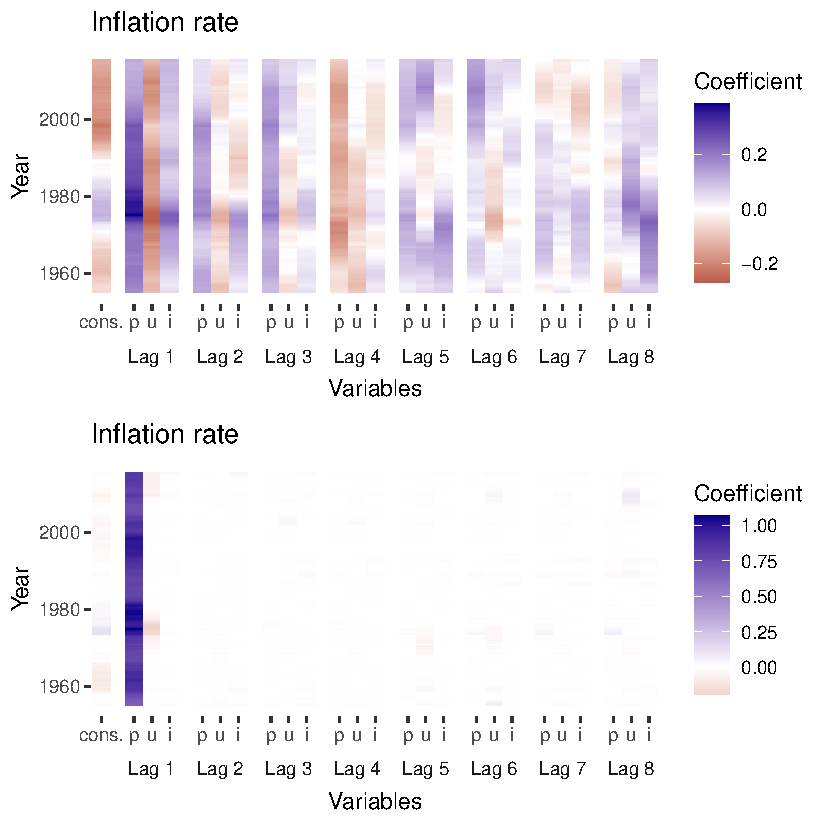
\includegraphics{Dynamic-Shrinkage-in-Bayesian-Structural-Time-Series-and-Vector-Autoregressive-Models_files/figure-latex/myfig72-1} 

}

\caption{Heat map representing estimated time-varying coefficients of the lagged VAR variables affecting inflation. In the upper panel, a VAR(8) model without shrinkage ($\Omega_\beta=1$) is presented. In this case, the signal is redistributed across all the predictors. In the lower panel, the same VAR(8) model is estimated when a severe shrinkage ($\Omega_\beta=0.2$) applies. Here, the signal is concentrated on the first lag of the dependent variable.}\label{fig:myfig72}
\end{figure}

\begin{figure}[H]

{\centering 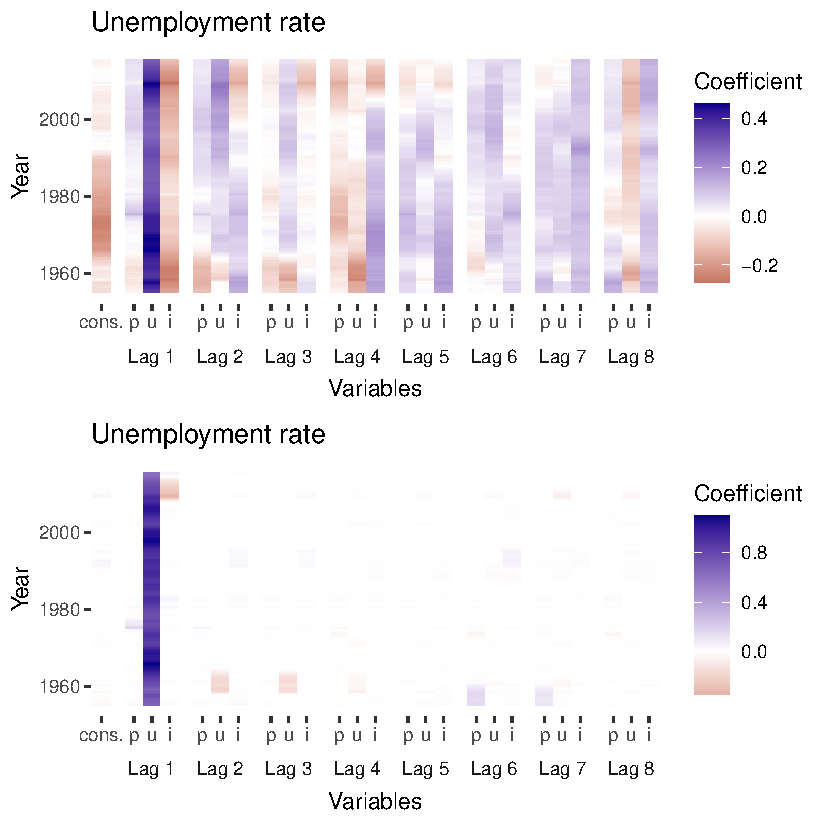
\includegraphics{Dynamic-Shrinkage-in-Bayesian-Structural-Time-Series-and-Vector-Autoregressive-Models_files/figure-latex/myfig73-1} 

}

\caption{Heat map representing estimated time-varying coefficients of the lagged VAR variables affecting unemployment rate. In the upper panel, a VAR(8) model without shrinkage ($\Omega_\beta=1$) is presented. In this case, the signal is redistributed across all the predictors. In the lower panel, the same VAR(8) model is estimated when a severe shrinkage ($\Omega_\beta=0.2$) applies. Here, the signal is concentrated on the first lag of the dependent variable.}\label{fig:myfig73}
\end{figure}

\begin{figure}[H]

{\centering 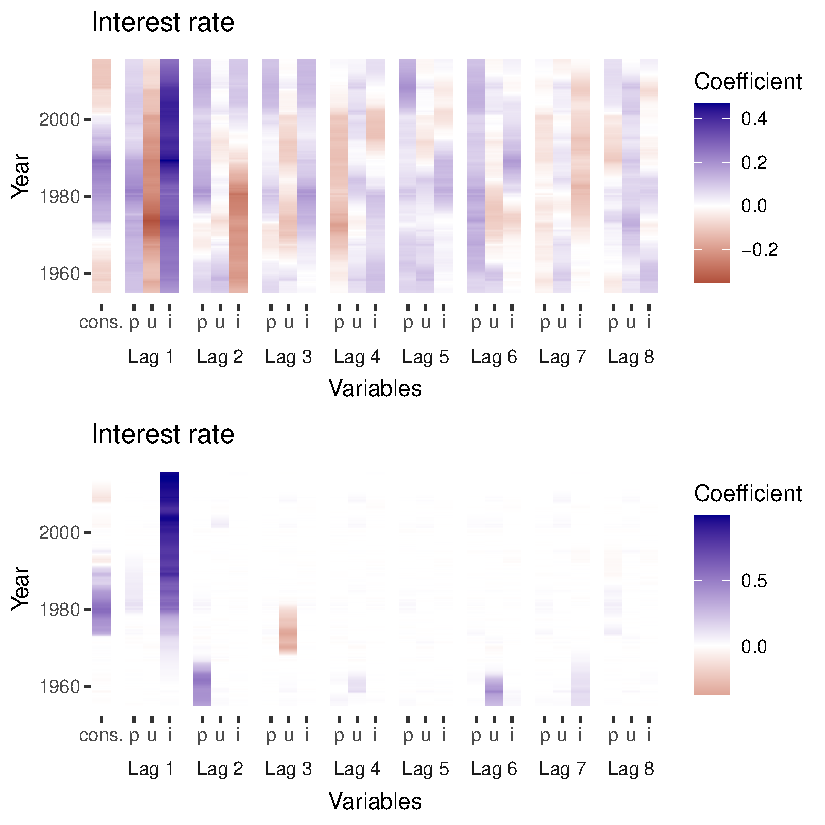
\includegraphics{Dynamic-Shrinkage-in-Bayesian-Structural-Time-Series-and-Vector-Autoregressive-Models_files/figure-latex/myfig74-1} 

}

\caption{Heat map representing estimated time-varying coefficients of the lagged VAR variables affecting interest rate. In the upper panel, a VAR(8) model without shrinkage ($\Omega_\beta=1$) is presented. In this case, the signal is redistributed across all the predictors. In the lower panel, the same VAR(8) model is estimated when a severe shrinkage ($\Omega_\beta=0.2$) applies. Here, the signal is concentrated on the first lag of the dependent variable.}\label{fig:myfig74}
\end{figure}

\begin{figure}[H]

{\centering 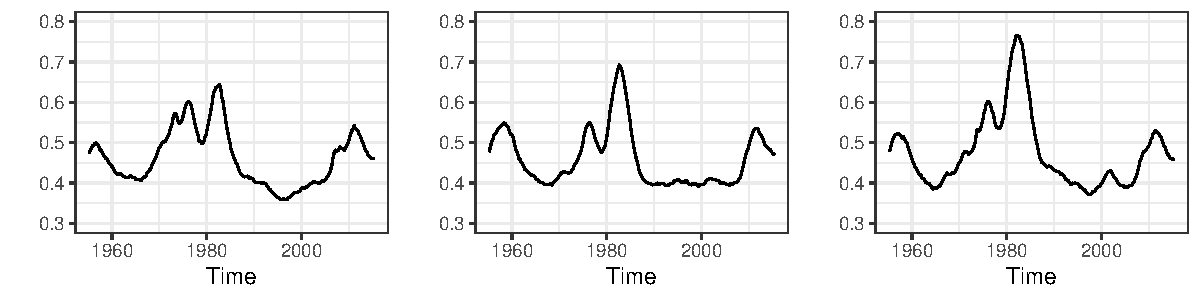
\includegraphics{Dynamic-Shrinkage-in-Bayesian-Structural-Time-Series-and-Vector-Autoregressive-Models_files/figure-latex/myfig502-1} 

}

\caption{MCMC approximation of the expected value of the residual standard deviations using precision sampler of inflation rate (left panel), unemployment rate (central panel), interest rate (right panel).}\label{fig:myfig502}
\end{figure}

We now test the out-of-sample performances of the models. Therefore,
one-step-ahead forecast distributions are approximated via MCMC for the
last ten periods of the series. The results are reported in Table
\ref{tab:mytab51} and they show that point forecasts improve for some
variables (interest rate and unemployment rate) when shrinkage applies.
Gains can be rather minor as in the case of inflation and unemployment
or very large as for the interest rate. Values of WMAPE and MASE are in
general acceptable. The huge values of MASE for interest rate are
motivated by the fact that interest rates have been kept close to the
zero lower bound in the effort of stimulating the economy after the 2008
financial crisis. Therefore the denominator of MASE is almost near zero
and the metric tends to be large by construction. The most impressive
gain lies in the SLPL. Indeed, noise reduction due to shrinkage of
unimportant coefficients toward zero lead to smaller credible intervals
and, thus, more precise estimates. From a visual standpoint, this effect
is shown in Figure \ref{fig:myfig71}.\\
Using the precision sampler we obtain very similar results but with a
significant gain in running time. For 1000 iterations the Dynamic SSVS
with a precision sampler scheme takes 170.76 seconds against the 1835.97
seconds of the Dynamic SSVS with double FFBS scheme. This fact leads to
new opportunities in the field of large TVP-VAR since it allows to deal
with a vast amount of coefficients in a reasonable amount of time and,
at the same time, it avoids overfitting thanks to dynamic shriankage.

\begin{table}[H]

\caption{\label{tab:mytab51}Dynamic SSVS with FFBS: performance comparison.}
\centering
\begin{tabular}[t]{>{}cccccc}
\toprule
  & $\Omega$ & RMSE & WMAPE & MASE & SLPL\\
\midrule
 & 0.2 & 0.121 & 0.159 & 0.998 & -18.665\\
\cmidrule{2-6}
\multirow[t]{-2}{*}{\centering\arraybackslash Inflation rate} & 1 & 0.127 & 0.135 & 0.846 & -25.84\\
\cmidrule{1-6}
 & 0.2 & 0.116 & 0.055 & 0.813 & -17.96\\
\cmidrule{2-6}
\multirow[t]{-2}{*}{\centering\arraybackslash Unemployment rate} & 1 & 0.16 & 0.065 & 0.966 & -25.821\\
\cmidrule{1-6}
 & 0.2 & 0.097 & 0.063 & 10.783 & -16.722\\
\cmidrule{2-6}
\multirow[t]{-2}{*}{\centering\arraybackslash Interest rate} & 1 & 0.235 & 0.155 & 26.465 & -27.216\\
\cmidrule{1-6}
 & 0.2 &  &  &  & -53.343\\
\cmidrule{2-6}
\multirow[t]{-2}{*}{\centering\arraybackslash Total} & 1 &  &  &  & -78.879\\
\bottomrule
\end{tabular}
\end{table}

\begin{table}[H]

\caption{\label{tab:mytab151}Dynamic SSVS with precision sampler: performance comparison.}
\centering
\begin{tabular}[t]{>{}cccccc}
\toprule
  & $\Omega$ & RMSE & WMAPE & MASE & SLPL\\
\midrule
 & 0.2 & 0.114 & 0.132 & 0.827 & -17.604\\
\cmidrule{2-6}
\multirow[t]{-2}{*}{\centering\arraybackslash Inflation rate} & 1 & 0.111 & 0.128 & 0.805 & -21.414\\
\cmidrule{1-6}
 & 0.2 & 0.11 & 0.053 & 0.791 & -17.219\\
\cmidrule{2-6}
\multirow[t]{-2}{*}{\centering\arraybackslash Unemployment rate} & 1 & 0.137 & 0.065 & 0.966 & -21.861\\
\cmidrule{1-6}
 & 0.2 & 0.062 & 0.042 & 7.119 & -14.875\\
\cmidrule{2-6}
\multirow[t]{-2}{*}{\centering\arraybackslash Interest rate} & 1 & 0.147 & 0.095 & 16.116 & -22.13\\
\cmidrule{1-6}
 & 0.2 &  &  &  & -49.697\\
\cmidrule{2-6}
\multirow[t]{-2}{*}{\centering\arraybackslash Total} & 1 &  &  &  & -65.405\\
\bottomrule
\end{tabular}
\end{table}

\begin{figure}[H]

{\centering 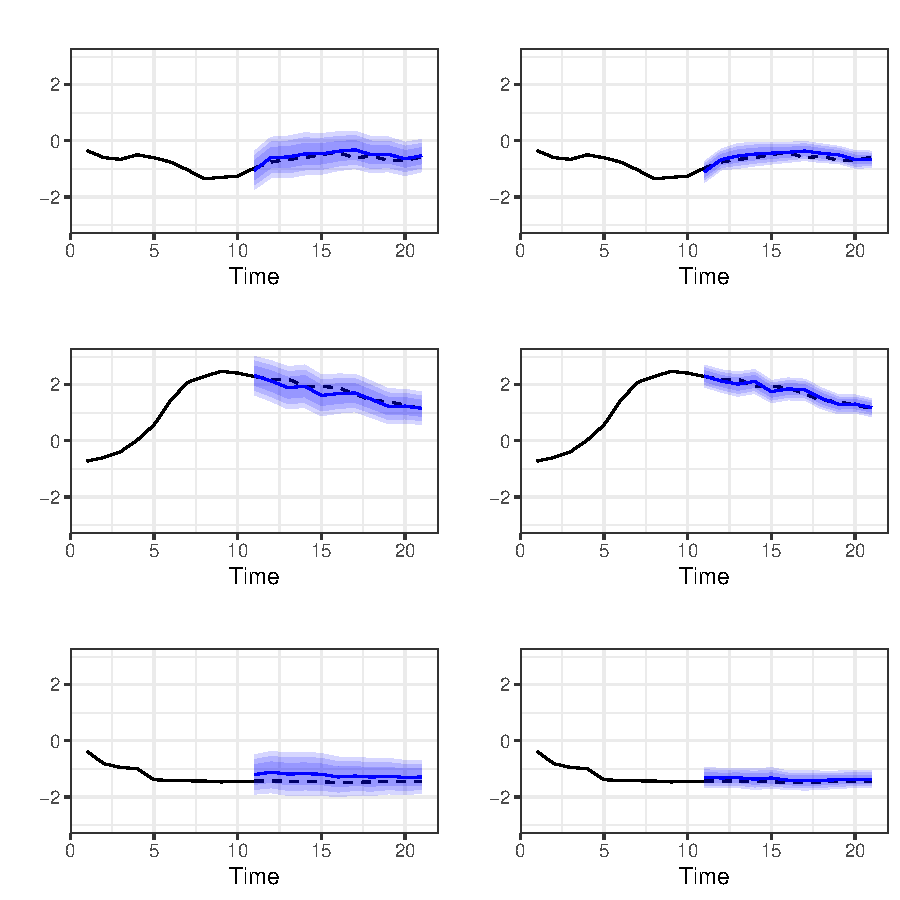
\includegraphics{Dynamic-Shrinkage-in-Bayesian-Structural-Time-Series-and-Vector-Autoregressive-Models_files/figure-latex/myfig71-1} 

}

\caption{TVP-VAR model comprising US inflation rate, unemployment rate and federal funds rate with 8 lags. One-step-ahead forecasts with credible intervals (blue) estimated using the precision sampler strategy and the true time series (black). On the left column, the graphs show forecasts generated by a TVP-VAR model with no shrinkage ($\Omega_\beta=1$), while on the right column forecasts are generated by a TVP-VAR model with severe shrinkage ($\Omega_\beta=0.2$). The latter presents smaller credible intervals.}\label{fig:myfig71}
\end{figure}

\begin{figure}[H]

{\centering 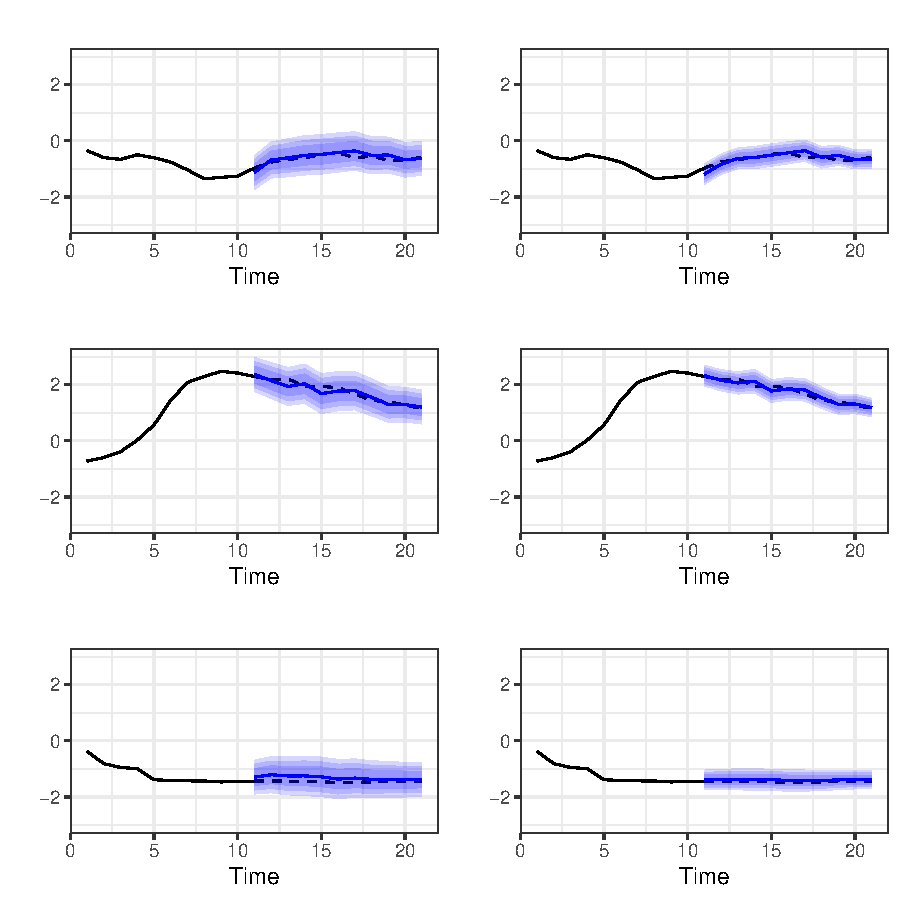
\includegraphics{Dynamic-Shrinkage-in-Bayesian-Structural-Time-Series-and-Vector-Autoregressive-Models_files/figure-latex/myfig722-1} 

}

\caption{TVP-VAR model comprising US inflation rate, unemployment rate and federal funds rate with 8 lags. One-step-ahead forecasts with credible intervals (blue) estimated using the precision sampler strategy and the true time series (black). On the left column, the graphs show forecasts generated by a TVP-VAR model with no shrinkage ($\Omega_\beta=1$), while on the right column forecasts are generated by a TVP-VAR model with severe shrinkage ($\Omega_\beta=0.2$). The latter presents smaller credible intervals.}\label{fig:myfig722}
\end{figure}

\section{Discussion}

With time-varying parameters, the risk of overfitting in VAR models is
round the corner. This prevents TVP-VAR model from being used in high
dimensions, limiting interesting modelling opportunities for applied
research. With the example described in the previous section, we show
the potentiality of Dynamic Spike-and-Slab process priors in mitigating
this problem. Our aim is to provide an approach to estimate large
TVP-VAR and Structural TVP-VAR that can be simultaneously fast and
precise. The combination of the precision sampler with the Dynamic SSVS
proved to be a valid strategy to achieve both goals. Thanks to dynamic
shrinkage priors it is possible to obtain a simpler model and achieve
important benefits in terms of interpretability. For what concern
forecasting, we shown that by removing noisy variables it is still
possible to preserve accuracy while reducing uncertainty. In addition,
here we decided to focus on forecasting as a way to validate model
performances, we do not exclude to expand this approach on causality and
impulse responses assessment features in further researches.
Nevertheless, the output of the \texttt{DSSTVPVAR\_SV} function in our
\texttt{dynamicshrink} package can be easily converted and used to
compute impulse response functions using the existing \texttt{bvarsv}
package. Another interesting fact we notice through the previous
analysis, which is true in principle, is that \(\boldsymbol{Y}_t\) is
less correlated with \(\boldsymbol{Y}_{t-h}\) when \(h\) increases. In
order to emphasize this phenomenon, dynamic shrinkage priors that induce
a greater penalization for \(h\) large could be developed. The work of
\protect\hyperlink{ref-legramanti2020bayesian}{Legramanti, Durante, and
Dunson} (\protect\hyperlink{ref-legramanti2020bayesian}{2020}) presents
a proposal in this direction for static problems. It would interesting
to translate it into a dynamic environment.

\chapter{My dynamicshrink R-package}\label{The dynamicshrink package}

The absence in literature of a unified \texttt{R}-package for dynamic
variable selection constitutes an important limit for empirical
research. With this thesis, we fill this gap by making available a set
of \texttt{R} functions that implement the estimation strategies
described in the previous chapters. Therefore, here we briefly introduce
our \texttt{dynamicshrink} package. This sort of experimental package
allows firstly to replicate the results obtained in previous sections
and, eventually, to perform further analysis on high dimensional time
series. The adjective ``experimental'' used here refers to the fact
that, even though the great efforts to make these functions high
performing, we acknowledge that there is room for improvements in terms
of computational time. The code, which is entirely written in
\texttt{R}, recalls for some specific tasks high-performing functions
provided by other popular packages. Reference \texttt{R} packages are:
\texttt{dlm}, \texttt{stochvol} and \texttt{matlib}, \texttt{MASS},
\texttt{Rcpp} and the \texttt{tidyverse}. Further developments in
\texttt{C} will eventually follow.\\
Below we present the list of the most useful functions complemented by a
brief description of them. In addition, a little helper is provided in
Appendix. Further details on these functions (and on the other
functions) can be found at the personal Github page of the author, along
with the rest of the code.

\newpage
\begin{table}[h!]
\begin{tabularx}{\textwidth}{|l|X|}
\texttt{DSSBSTS\_SV}          & Dynamic Spike-and-Slab Bayesian Structural Time Series with log-normal AR(1) stochastic volatility \\
\texttt{DSSBSTS\_DF}          & Dynamic Spike-and-Slab Bayesian Structural Time Series with discount factor model for time-varying variances \\
\texttt{MCMC.out} & Compute meaningful statistics from the output of \texttt{DSSBSTS\_SV} and \texttt{DSSBSTS\_DF} \\
\texttt{DEMVS} & Dynamic Expectation-Maximization Variable Selection with discount factor model for time-varying variances \\
\texttt{DEMVS\_PS} & Dynamic Expectation-Maximization Variable Selection with log-normal AR(1) stochastic volatility estimated via Particle Smoothing (PS)\\
\texttt{DEMVS.Quarterly} \\ \texttt{DEMVS.Monthly} & Dynamic Expectation-Maximization Variable Selection for Bayesian Structural Time Series with log-normal AR(1) stochastic volatility estimated via Particle Smoothing (PF). The functions are respectively built for quarterly and monthly data.\\
\texttt{DSSTVPVAR\_SV} & Dynamic Stochastic Search Variable Selection for Time-Varying Parameter Vector Autoregressive models with Stochastic Volatility.\\
\texttt{MCMC.TVPVAR.out} & Compute meaningful statistics from the output of \texttt{DSSTVPVAR\_SV}\\
\end{tabularx}
\end{table}

\newpage
\begin{table}[h!]
\begin{tabularx}{\textwidth}{|l|X|}
\texttt{sparse.data.sim} & Generates dynamic sparse time series data.\\
\texttt{varplot} & Generates the plot of the volatility process \\
\texttt{Indicatorplot} & Generates the plot of the indicator variables \\
\texttt{Coef.compare.plot} & Generates the plot the regression coefficients. It can be used for comparisons \\
\texttt{SeasTrendSlope.plot} & Generates three plots concerning the time series seasonality, trend and trend's slope. \\
\texttt{SeasTrendReg.plot} & Generates three plots concerning the time series regression component, seasonal component and trend component estimated using Dynamic SSVS.\\
\texttt{SeasTrendReg.plot.1} &  Generates three plots concerning the time series regression component, seasonal component and trend component estimated using Dynamic EMVS.\\
\texttt{Active.coef.plot} & Generates a plot indicating how many coefficients result active at each period in time. \\
\texttt{Forecastplot} & Compares forecasts with the actual series. Developed for BSTS models. \\
\texttt{Forecastplot.TVP.VAR} & Compares forecasts with the actual series. Developed for TVP-VAR models. \\
\texttt{DSS\_PRECISIONSAMPLER} & Dynamic Stochastic Search Variable Selection for Time-Varying Parameter Vector Autoregressive models with Stochastic Volatility. The FFBS step is replaced by a precision sampler.\\
\texttt{DSSTVP\_PRECISIONSAMPLER} & Dynamic Stochastic Search Variable Selection for Time-Varying Parameter Vector Autoregressive models with Stochastic Volatility. The FFBS step is replaced by a precision sampler.
\end{tabularx}
\end{table}

\newpage

Here we discuss briefly how the package works presenting the code used
for the simulations study on quasi-synthetic data. Let's thus simulate a
TVP regression model with 20 predictors of which only the first four are
truly relevant using the function \texttt{sparse.data.sim}. We label
data generated through this function as \texttt{synthetic.y} and then we
add to then Airpassengers data in lags and rescaled by ten. We rescaled
real data to adapt them to the scale of simulated data, note that
results would not be affected if data are not rescaled. The true model's
parameter are labeled \texttt{true\_b} and \texttt{true\_ind}.

\begin{Shaded}
\begin{Highlighting}[]
\NormalTok{sim }\OtherTok{=} \FunctionTok{sparse.data.sim}\NormalTok{(}\AttributeTok{TIME=}\DecValTok{144}\NormalTok{,}\AttributeTok{P=}\DecValTok{4}\NormalTok{,}\AttributeTok{FP=}\DecValTok{16}\NormalTok{,}
                     \AttributeTok{phi0=}\DecValTok{0}\NormalTok{,}\AttributeTok{phi1=}\FloatTok{0.98}\NormalTok{,}\AttributeTok{lambda1=}\FloatTok{0.1}\NormalTok{,}\AttributeTok{v=}\DecValTok{0}\NormalTok{,}\AttributeTok{seed=}\DecValTok{100}\NormalTok{)}
\NormalTok{synthetic.y }\OtherTok{=}\NormalTok{ sim}\SpecialCharTok{$}\NormalTok{y}
\NormalTok{X }\OtherTok{=}\NormalTok{ sim}\SpecialCharTok{$}\NormalTok{X}
\NormalTok{real.y }\OtherTok{=} \FunctionTok{log}\NormalTok{(}\FunctionTok{as.numeric}\NormalTok{(AirPassengers))}
\NormalTok{y }\OtherTok{=}\NormalTok{ real.y}\SpecialCharTok{*}\DecValTok{10}\SpecialCharTok{+}\NormalTok{synthetic.y }
\NormalTok{true\_b }\OtherTok{=}\NormalTok{ sim}\SpecialCharTok{$}\NormalTok{true\_b}
\NormalTok{true\_ind }\OtherTok{=}\NormalTok{ sim}\SpecialCharTok{$}\NormalTok{true\_ind}
\end{Highlighting}
\end{Shaded}

The estimation of the models parameters can be carried out using one of
the following functions: \texttt{DSSBSTS\_SV}, \texttt{DSSBSTS\_DF} or
\texttt{DEMVS.Monthly} whose general functionality is introduced in the
tables above. The positive note here is that, even though they
implements different strategies their usage is very similar, therefore
we focus on the first function mentioned before to provide an overall
guidance. The arguments of the function are self-explanatory. The
model's hyperparameters are \texttt{phi1}, \texttt{phi0},
\texttt{lambda1}, \texttt{lambda0} and \texttt{OMEGA}, the starting
values of the indicators, \texttt{gamma0}, and the volatility,
\texttt{v0}, and the structural components, \texttt{S} and \texttt{U}.
Moreover, \texttt{sig2u}, \texttt{sig2d}, \texttt{sig2tau} are the
variances of, respectively, the trend, the slope and the seasonal
factor. Note that the value of \texttt{S} is equal to the number of
seasonal factors to be estimated i.e.~\(S-1\) where \(S\) is equal for
example to 12 in monthly time series. On the other hand, \texttt{U} may
be equal to 2 if our base model is a linear growth model or equal to 1
if it is a local level model. Alternatively to \texttt{U}=1, one can add
a constant to the matrix of predictors and set \texttt{ACTIVATE=TRUE}
which means that the indicator of the first predictor will be always set
equal to one. This latter option is useful also when we do not want to
shrinkage an important predictor. In the latter case that predictors has
to stay in the first column of \texttt{X}. If present, \texttt{new.X}
contains future values of the predictors, \(\boldsymbol{x}_{t+1}\),
which are used for one-step-ahead forecasting. Finally
\texttt{start\_params} and \texttt{start\_latent} are two objects
defined in the \texttt{stochvol} package and they refer to the starting
parameters and starting latent values of a stochastic volatility model.

\begin{Shaded}
\begin{Highlighting}[]
\FunctionTok{set.seed}\NormalTok{(}\DecValTok{1}\NormalTok{)}
\NormalTok{ssvs.bsts }\OtherTok{=} \FunctionTok{DSSBSTS\_SV}\NormalTok{(}\AttributeTok{y=}\NormalTok{y,}\AttributeTok{X=}\NormalTok{X,}\AttributeTok{N=}\DecValTok{1000}\NormalTok{,}\AttributeTok{S=}\DecValTok{11}\NormalTok{,}\AttributeTok{U=}\DecValTok{2}\NormalTok{,}
                     \AttributeTok{phi0=}\DecValTok{0}\NormalTok{,}\AttributeTok{phi1=}\FloatTok{0.98}\NormalTok{,}\AttributeTok{gamma0=}\FloatTok{0.5}\NormalTok{,}\AttributeTok{v0=}\FloatTok{0.25}\NormalTok{,}
                     \AttributeTok{sig2u=}\FloatTok{0.1}\NormalTok{,}\AttributeTok{sig2d=}\FloatTok{0.1}\NormalTok{,}\AttributeTok{sig2tau=}\FloatTok{0.1}\NormalTok{,}
                     \AttributeTok{lambda0=}\FloatTok{0.01}\NormalTok{,}\AttributeTok{lambda1=}\FloatTok{0.1}\NormalTok{,}\AttributeTok{OMEGA=}\FloatTok{0.2}\NormalTok{,}
\NormalTok{                     start\_params,start\_latent,new.X,}\AttributeTok{activate=}\NormalTok{F)}
\end{Highlighting}
\end{Shaded}

This function returns a huge list of objects of which the most important
are the samples generate by the Markov Chain. These samples are indeed
stored in arrays whose interpretation is not immediate, therefore we
need to convert them into some meaningful statistics. This is done by
the function \texttt{MCMC.out} which returns the sample means and the
sample variances. Here we just plug the name of the function used for
model estimation and the number of samples to burn-in. Note that this
function is already endowed in many other functions such as plot
functions. Moreover, the functions carrying out the precision sampler do
not need this passage, but they directly return the mean and the
variance of the MCMC estimates.

\begin{Shaded}
\begin{Highlighting}[]
\NormalTok{mcmc }\OtherTok{=} \FunctionTok{MCMC.out}\NormalTok{(}\AttributeTok{fun=}\NormalTok{ssvs.bsts,}\AttributeTok{burn=}\DecValTok{200}\NormalTok{)}
\end{Highlighting}
\end{Shaded}

Once the model parameters are estimated, there are several useful tool
for visualization. For example, \texttt{Coef.compare.plot} provides the
plot of the estimated regression coefficients and, if \texttt{trueb} is
not missing, it compares them to their true values or, if \texttt{trueb}
is equal to coefficients estimated with other model's specifications, it
compares the two. \texttt{column} indicates the column of interest of
the regression matrix and if for example \texttt{column=1} the plot of
\(\beta_{1:T,1}\) will be generated. Furthermore, when we use the
Dynamic EMVS instead of the Dynamic SSVS, then \texttt{EMVS} should be
explicated. If we want dates on the x-axis then \texttt{time} must be
equal to a date vector of the same length of \texttt{y}, otherwise if
\texttt{time} is missing the x-axis will be a vector of natural numbers.
Figure \ref{fig:myfig7} is generated from the following command for
\(i=1,...,6\).

\begin{Shaded}
\begin{Highlighting}[]
\FunctionTok{Coef.compare.plot}\NormalTok{(}\AttributeTok{trueb=}\NormalTok{true\_b,}\AttributeTok{column=}\NormalTok{i,}\AttributeTok{fun=}\NormalTok{ssvs.bsts,}\AttributeTok{burn=}\DecValTok{200}\NormalTok{,time,EMVS)}
\end{Highlighting}
\end{Shaded}

Similarly, \texttt{Indicatorplot}, \texttt{varplot} provides plots of
the MCMC approximation of the expected values of the indicators and the
variance. \texttt{Active.coef.plot} instead shows how many variables are
relevant at any moment in time. If structural time series components are
estimated, they can be represented by the two following function which
plots respectively the trend, the seasonality and the regression
component. The following generates Figure \ref{fig:myfig14}

\begin{Shaded}
\begin{Highlighting}[]
\FunctionTok{SeasTrendReg.plot}\NormalTok{(ssvs.bsts,}\AttributeTok{S=}\DecValTok{11}\NormalTok{,}\AttributeTok{U=}\DecValTok{2}\NormalTok{,}\AttributeTok{burn=}\DecValTok{200}\NormalTok{)}
\end{Highlighting}
\end{Shaded}

Forecasts one-step-ahead, two-step-ahead and so on are visualized via
the function \texttt{Forecastplot}, for univariate time series the
latter provides a comparison between realizations and point forecasts
along with their credible intervals. Below we present an example. The
time series \texttt{y} is plotted from \texttt{from} to \texttt{to},
whereas the forecasts are plotted from \texttt{start\_fc} to
\texttt{to}. This allows to show the path of the dependent variable
before forecasting starts.

\begin{Shaded}
\begin{Highlighting}[]
\FunctionTok{Forecastplot}\NormalTok{(y,from,to,start\_fc,fc.f,fc.Q,ub,lb,timeframe)}
\end{Highlighting}
\end{Shaded}

In addition, the package provides all the metrics relevant for
comparisons such as SSE, Hamming Distance, MASE, MAFE, RMSE, LPDS, FP,
FN etc. The case in which the time series does not show evident time
series structural component can be estimated by the same functions with
missing \texttt{S} and \texttt{U} or, according to need, by
\texttt{DSS\_PRECISIONSAMPLER}, \texttt{DEMVS} and \texttt{DEMVS\_PS}.
In general, as already mentioned, the usage is similar among these
functions.\\
For the multivariate case, instead, another set of functions is
envisaged. The relevant functions here are: \texttt{DSSTVPVAR\_SV} which
estimates the Time-Varying Parameter Structural VAR model of
\protect\hyperlink{ref-Primicieri_2005}{Primiceri}
(\protect\hyperlink{ref-Primicieri_2005}{2005}) whit shrinkage,
\texttt{DSSTVP\_PRECISIONSAMPLER\_VAR} and
\texttt{DSSTVP\_PRECISIONSAMPLER\_SVAR} that estimates respectively the
Time-Varying Parameter VAR and Structural VAR models with the precision
sampler. As we can see from the code below, the overall structure of the
command is similar to the one mentioned before. \texttt{X} is the
regression matrix with the variables of the VAR model. If
\texttt{constant=TRUE} then a constant will be added to the model. Now
we have two hyperparameters \texttt{OMEGA} which are respectively
\(\Omega_\alpha\) and \(\Omega_\beta\). In this experimental version of
the package the function are built in order to provide just
one-step-ahead forecasts, thus \texttt{step\_ahead=1}, however we do not
exclude further developments to extend the number of steps ahead.
Finally, together with the starting value of the variances, \texttt{v0},
the starting value of the covariances, \texttt{cov0}, should be set. We
decided to keep it simple and let all the covariances to have the same
starting values.

\begin{Shaded}
\begin{Highlighting}[]
\FunctionTok{DSSTVPVAR\_SV}\NormalTok{(X,constant,N,lags,}
             \AttributeTok{step\_ahead=}\DecValTok{1}\NormalTok{,gamma0,phi0,v0,cov0,phi1,}
\NormalTok{             OMEGA.A,OMEGA.B,lambda0,lambda1,}
\NormalTok{             start\_params,start\_latent)}
\end{Highlighting}
\end{Shaded}

Ad-hoc functions are created to deal with the output of
\texttt{DSSTVPVAR\_SV}, these are very similar to the ones mentioned
above and they are \texttt{MCMC.TVP.out} for extracting the meaningful
statistics, \texttt{Forecastplot.TVP.VAR} to plot forecasts and
\texttt{lpds\_multi} which is the multivariate version of the
\texttt{lpds} command for Log-Predicitive Density Sum comparison. Again
\texttt{DSSTVP\_PRECISIONSAMPLER\_VAR} and
\texttt{DSSTVP\_PRECISIONSAMPLER\_SVAR} return directly the mean and the
variances of the estimates.

\backmatter

\chapter{Bibliography}

\hypertarget{refs}{}
\begin{CSLReferences}{1}{0}
\leavevmode\vadjust pre{\hypertarget{ref-AM_1974}{}}%
Andrews, D. F., and C. L. Mallows. 1974. {``Scale Mixtures of Normal
Distributions.''} \emph{Journal of the Royal Statistical Society. Series
B (Methodological)} 36 (1): 99--102.

\leavevmode\vadjust pre{\hypertarget{ref-Belmonte}{}}%
Belmonte, M. A. G., G. Koop, and D. Korobilis. 2014. {``{Hierarchical
Shrinkage in Time‐Varying Parameter Models}.''} \emph{Journal of
Forecasting} 33 (1): 80--94.

\leavevmode\vadjust pre{\hypertarget{ref-bitto_fruhwirth-schnatter_2019}{}}%
Bitto, A., and S. Fruhwirth-Schnatter. 2019. {``Achieving Shrinkage in a
Time-Varying Parameter Model Framework.''} \emph{Journal of
Econometrics} 210: 75--97.

\leavevmode\vadjust pre{\hypertarget{ref-bitto2018achieving}{}}%
Bitto, A., and S. Frühwirth-Schnatter. 2018. {``Achieving Shrinkage in a
Time-Varying Parameter Model Framework.''}

\leavevmode\vadjust pre{\hypertarget{ref-CANOVA_1993}{}}%
Canova, Fabio, and Harris Dellas. 1993. {``Trade Interdependence and the
International Business Cycle.''} \emph{Journal of International
Economics} 34 (1-2): 23--47.

\leavevmode\vadjust pre{\hypertarget{ref-CK_1994}{}}%
Carter, C. K., and R. Kohn. 1994. {``On Gibbs Sampling for State Space
Models.''} \emph{Biometrika} 81 (3): 541--53.

\leavevmode\vadjust pre{\hypertarget{ref-Chan_2018}{}}%
Chan, J., and E. Eisenstat. 2018. {``Bayesian Model Comparison for
Time-Varying Parameter VARs with Stochastic Volatility.''} \emph{Journal
of Applied Econometrics} 33 (4): 509--32.

\leavevmode\vadjust pre{\hypertarget{ref-chan_jeliazkov_2009}{}}%
Chan, J., and I. Jeliazkov. 2009. {``Efficient Simulation and Integrated
Likelihood Estimation in State Space Models.''} \emph{International
Journal of Mathematical Modelling and Numerical Optimisation} 1 (1/2):
101.

\leavevmode\vadjust pre{\hypertarget{ref-CP_2020}{}}%
Chopin, N., and O. Papaspiliopoulos. 2020. {``An Introduction to
Sequential Monte Carlo,''} January.

\leavevmode\vadjust pre{\hypertarget{ref-CR_2015}{}}%
Clark, T. E., and F. Ravazzolo. 2015. {``Macroeconomic Forecasting
Performance Under Alternative Specifications of Time-Varying
Volatility.''} \emph{Journal of Applied Econometrics} 30 (4): 551--75.

\leavevmode\vadjust pre{\hypertarget{ref-COGLEY2005262}{}}%
Cogley, T., and T. J. Sargent. 2005. {``Drifts and Volatilities:
Monetary Policies and Outcomes in the Post WWII US.''} \emph{Review of
Economic Dynamics} 8 (2): 262--302.

\leavevmode\vadjust pre{\hypertarget{ref-Durbin_K2002}{}}%
Durbin, J., and S. J. Koopman. 2002. {``A Simple and Efficient
Simulation Smoother for State Space Time Series Analysis.''}
\emph{Biometrika} 89 (3): 603--15.

\leavevmode\vadjust pre{\hypertarget{ref-EJC_2016}{}}%
Eisenstat, E., J. Chan, and R. Strachan. 2014. {``Stochastic Model
Specification Search for Time-Varying Parameter VARs.''} \emph{SSRN
Electronic Journal}, January.
\url{https://doi.org/10.2139/ssrn.2403560}.

\leavevmode\vadjust pre{\hypertarget{ref-fan2010reversible}{}}%
Fan, Y., and S. A. Sisson. 2010. {``Reversible Jump Markov Chain Monte
Carlo.''}

\leavevmode\vadjust pre{\hypertarget{ref-fruhwirth-schnatter_1994}{}}%
Fruhwirth-Schnatter, S. 1994. {``Data Augmentation and Dynamic Linear
Models.''} \emph{Journal of Time Series Analysis} 15 (2): 183--202.

\leavevmode\vadjust pre{\hypertarget{ref-G_1986a}{}}%
George, E. I. 1986a. {``Combining Minimax Shrinkage Estimators.''}
\emph{Journal of the American Statistical Association} 81 (394).

\leavevmode\vadjust pre{\hypertarget{ref-G_1986b}{}}%
---------. 1986b. {``Minimax Multiple Shrinkage Estimation.''} \emph{The
Annals of Statistics} 14 (1).

\leavevmode\vadjust pre{\hypertarget{ref-GM_1993}{}}%
George, E. I., and R. E. McCulloch. 1993. {``Variable Selection via
Gibbs Sampling.''} \emph{Journal of the American Statistical
Association} 88 (423): 881--89.

\leavevmode\vadjust pre{\hypertarget{ref-GM_1997}{}}%
---------. 1997. {``Approaches for Bayesian Variable Selection.''}
\emph{Statistica Sinica} 7 (2): 339--73.

\leavevmode\vadjust pre{\hypertarget{ref-GDW_2004}{}}%
Godsill, S. J., A. Doucet, and M. West. 2004. {``Monte Carlo Smoothing
for Nonlinear Time Series.''} \emph{Journal of the American Statistical
Association} 99: 156--68.

\leavevmode\vadjust pre{\hypertarget{ref-G_1995}{}}%
Green, P. J. 1995. {``Reversible Jump Markov Chain Monte Carlo
Computation and Bayesian Model Determination.''} \emph{Biometrika} 82
(4): 711--32.

\leavevmode\vadjust pre{\hypertarget{ref-KALLI2014779}{}}%
Kalli, M., and J. E. Griffin. 2014. {``Time-Varying Sparsity in Dynamic
Regression Models.''} \emph{Journal of Econometrics} 178 (2): 779--93.

\leavevmode\vadjust pre{\hypertarget{ref-SV_2016}{}}%
Kastner, G. 2016. {``Dealing with Stochastic Volatility in Time Series
Using the r Package Stochvol.''} \emph{Journal of Statistical Software}
69 (5): 1--30.

\leavevmode\vadjust pre{\hypertarget{ref-KASTNER2014408}{}}%
Kastner, G., and S. Frühwirth-Schnatter. 2014.
{``Ancillarity-Sufficiency Interweaving Strategy (ASIS) for Boosting
MCMC Estimation of Stochastic Volatility Models.''} \emph{Computational
Statistics and Data Analysis} 76: 408--23.

\leavevmode\vadjust pre{\hypertarget{ref-KSC_1998}{}}%
Kim, S., N. Shephard, and S. Chib. 1998. {``Stochastic Volatility:
Likelihood Inference and Comparison with ARCH Models.''} \emph{The
Review of Economic Studies} 65 (3): 361--93.

\leavevmode\vadjust pre{\hypertarget{ref-GOOGLE_TRENDS}{}}%
Koop, G., and L. Onorante. 2019. {``Macroeconomic Nowcasting Using
Google Probabilities.''} In \emph{Topics in Identification, Limited
Dependent Variables, Partial Observability, Experimentation, and
Flexible Modeling: Part a}, 40A:17--40. Emerald Publishing Ltd.

\leavevmode\vadjust pre{\hypertarget{ref-Korob_VAR}{}}%
Korobilis, D. 2013. {``VAR Forecasting Using Bayesian Variable
Selection.''} \emph{Journal of Applied Econometrics} 28 (2): 204--30.

\leavevmode\vadjust pre{\hypertarget{ref-KC_2014}{}}%
Kroese, D. P., and J. C. Chan. 2014. \emph{Statistical Modeling and
Computation}. Springer, New York, 2014.

\leavevmode\vadjust pre{\hypertarget{ref-legramanti2020bayesian}{}}%
Legramanti, S., D. Durante, and D. B Dunson. 2020. {``Bayesian
Cumulative Shrinkage for Infinite Factorizations.''}

\leavevmode\vadjust pre{\hypertarget{ref-LW_2001}{}}%
Liu, J., and M. West. 2001. {``Combined Parameter and State Estimation
in Simulation-Based Filtering.''} In \emph{Sequential Monte Carlo
Methods in Practice}.

\leavevmode\vadjust pre{\hypertarget{ref-MCCAUSLAND2011199}{}}%
McCausland, W. J., S. Miller, and D. Pelletier. 2011. {``Simulation
Smoothing for State--Space Models: A Computational Efficiency
Analysis.''} \emph{Computational Statistics and Data Analysis} 55 (1):
199--212.

\leavevmode\vadjust pre{\hypertarget{ref-FREDMD}{}}%
McCracken, M. W., and S. Ng. 2016. {``{FRED-MD: A Monthly Database for
Macroeconomic Research}.''} \emph{Journal of Business \& Economic
Statistics} 34 (4): 574--89.

\leavevmode\vadjust pre{\hypertarget{ref-FREDQD}{}}%
McCracken, Michael W., and Serena Ng. 2021. {``{FRED-QD: A Quarterly
Database for Macroeconomic Research}.''} \emph{Review} 103 (1): 1--44.

\leavevmode\vadjust pre{\hypertarget{ref-MB_1988}{}}%
Mitchell, T. J., and J. J. Beauchamp. 1988. {``Bayesian Variable
Selection in Linear Regression.''} \emph{Journal of the American
Statistical Association} 83 (404): 1023--32.

\leavevmode\vadjust pre{\hypertarget{ref-Nakajima2013a}{}}%
Nakajima, J., and M. West. 2013. {``Bayesian Analysis of Latent
Threshold Dynamic Models.''} \emph{Journal of Business \& Economic
Statistics} 31 (2): 151--64.

\leavevmode\vadjust pre{\hypertarget{ref-ning2021mbsts}{}}%
Ning, N., and J. Qiu. 2021. {``The Mbsts Package: Multivariate Bayesian
Structural Time Series Models in r.''}

\leavevmode\vadjust pre{\hypertarget{ref-OS_2009}{}}%
O'Hara, R. B., and M. J. Sillanpää. 2009. {``{A review of Bayesian
variable selection methods: what, how and which}.''} \emph{Bayesian
Analysis} 4 (1): 85--117.

\leavevmode\vadjust pre{\hypertarget{ref-PC_2008}{}}%
Park, T., and G. Casella. 2008. {``The Bayesian Lasso.''} \emph{Journal
of the American Statistical Association} 103 (482): 681--86.

\leavevmode\vadjust pre{\hypertarget{ref-DLM}{}}%
Petris, G. 2010. {``An {R} Package for Dynamic Linear Models.''}
\emph{Journal of Statistical Software} 36 (12): 1--16.

\leavevmode\vadjust pre{\hypertarget{ref-petris_petrone_campagnoli_2009}{}}%
Petris, G., S. Petrone, and P. Campagnoli. 2009. {``Dynamic Linear
Models.''} \emph{Dynamic Linear Models with R}, 31--84.

\leavevmode\vadjust pre{\hypertarget{ref-Primicieri_2005}{}}%
Primiceri, G. E. 2005. {``Time Varying Structural Vector Autoregressions
and Monetary Policy.''} \emph{The Review of Economic Studies} 72 (3):
821--52.

\leavevmode\vadjust pre{\hypertarget{ref-R_2013}{}}%
Rockova, V. 2013. {``{Bayesian Variable Selection in High-dimensional
Applications}.''}

\leavevmode\vadjust pre{\hypertarget{ref-RG_2014}{}}%
Rockova, V., and E. I. George. 2014. {``EMVS: The EM Approach to
Bayesian Variable Selection.''} \emph{Journal of the American
Statistical Association} 109 (506): 828--46.

\leavevmode\vadjust pre{\hypertarget{ref-rockova_mcalinn_2021}{}}%
Rockova, V., and K. McAlinn. 2021a. {``Dynamic Variable Selection with
Spike-and-Slab Process Priors.''} \emph{Bayesian Analysis} 16 (1).

\leavevmode\vadjust pre{\hypertarget{ref-RM_2020}{}}%
---------. 2021b. {``Dynamic Variable Selection with Spike-and-Slab
Process Priors - Supplementary Material.''} \emph{Bayesian Analysis}.

\leavevmode\vadjust pre{\hypertarget{ref-scott_varian_2013}{}}%
Scott, S. L., and H. R. Varian. 2013. {``Predicting the Present with
Bayesian Structural Time Series.''} \emph{SSRN Electronic Journal}.

\leavevmode\vadjust pre{\hypertarget{ref-S_1994}{}}%
Shephard, N. 1994. {``Partial Non-Gaussian State Space.''}
\emph{Biometrika} 81 (1): 115--31.

\leavevmode\vadjust pre{\hypertarget{ref-SIMS_1980}{}}%
Sims, C. A. 1980. {``Macroeconomics and Reality.''} \emph{Econometrica}
48 (1): 1--48.

\leavevmode\vadjust pre{\hypertarget{ref-CS_2001}{}}%
Stock, J. H. 2001. {``Evolving Post-World War II u.s. Inflation
Dynamics.''} \emph{NBER Macroeconomics Annual} 16: 379--87.

\leavevmode\vadjust pre{\hypertarget{ref-T_1996}{}}%
Tibshirani, R. 1996. {``Regression Shrinkage and Selection via the
Lasso.''} \emph{Journal of the Royal Statistical Society. Series B
(Methodological)} 58 (1): 267--88.

\leavevmode\vadjust pre{\hypertarget{ref-varian_choi_2009}{}}%
Varian, H., and H. Choi. 2009a. {``Predicting the Present with Google
Trends.''} \emph{SSRN Electronic Journal}.

\leavevmode\vadjust pre{\hypertarget{ref-CV_2009}{}}%
---------. 2009b. {``Predicting the Present with Google Trends.''}
\emph{Economic Record} 88 (April).

\leavevmode\vadjust pre{\hypertarget{ref-MASS}{}}%
Venables, W. N., and B. D. Ripley. 2002. \emph{Modern Applied Statistics
with s}. Fourth. New York: Springer.

\leavevmode\vadjust pre{\hypertarget{ref-WH_1997}{}}%
West, M., and J. Harrison. 1997. \emph{Bayesian Forecasting and Dynamic
Models (2nd Ed.)}. Berlin, Heidelberg: Springer-Verlag.

\leavevmode\vadjust pre{\hypertarget{ref-TIDYVERSE}{}}%
Wickham, Hadley, Mara Averick, Jennifer Bryan, Winston Chang, Lucy
D'Agostino McGowan, Romain François, Garrett Grolemund, et al. 2019.
{``Welcome to the {tidyverse}.''} \emph{Journal of Open Source Software}
4 (43): 1686.

\leavevmode\vadjust pre{\hypertarget{ref-Woodburry}{}}%
William, W. H. 1989. {``Updating the Inverse of a Matrix.''} \emph{SIAM
Review} 31 (2): 221--39.

\leavevmode\vadjust pre{\hypertarget{ref-WL_2000}{}}%
Wong, C. S., and W. K. Li. 2000. {``On a Mixture Autoregressive
Model.''} \emph{Journal of the Royal Statistical Society. Series B
(Statistical Methodology)} 62 (1): 95--115.

\leavevmode\vadjust pre{\hypertarget{ref-YM_2011}{}}%
Yu, Y., and X. Meng. 2011. {``To Center or Not to Center: That Is Not
the Question---an Ancillarity--Sufficiency Interweaving Strategy (ASIS)
for Boosting MCMC Efficiency.''} \emph{Journal of Computational and
Graphical Statistics} 20 (3): 531--70.

\leavevmode\vadjust pre{\hypertarget{ref-zellner_1986}{}}%
Zellner, A. 1986. {``On Assessing Prior Distributions and Bayesian
Regression Analysis with g-Prior Distributions.''} \emph{Bayesian
Inference and Decision Techniques: Essays in Honor of Bruno de Finetti}.

\end{CSLReferences}

\chapter{Acknowledgement}

A conclusione di questo elaborato, desidero ringraziare tutte le persone
che mi hanno supportato nella stesura di questa tesi e, più in generale,
nel mio percorso accademico.

In particolar modo, voglio ringraziare la Professoressa Sonia Petrone
che ha saputo guidarmi, con suggerimenti pratici, nelle ricerche e nella
stesura dell'elaborato. Il suo lavoro meticoloso di revisione di questa
tesi ha contribuito immensamente a migliorarne l'esposizione.

Ringrazio inoltre il Professor Marco Bonetti che è stato mio mentore
presso il BIDSA per avermi trasmesso la sua passione per la statistica e
la ricerca.

Ringrazio infinitamente mia madre e mio padre, senza il loro supporto,
questo lavoro di tesi non esisterebbe nemmeno.

Infine voglio ringraziare i miei amici storici e quelli conosciuti in
Bocconi per tutti i momenti passati insieme. Un riconoscimento speciale
va al mio amico e coinquilino Yuri, per essere riuscito a strapparmi una
risata anche nei momenti più ardui vissuti durante la magistrale, ed
alla mia ragazza Lilia, per essermi stata a fianco in questi mesi.

\appendix

\chapter{Appendix}

\section{Dynamic Spike-and-Slab with Laplace priors}\label{Appendix A.1}

As already mentioned in the text, using a Laplace spike instead of a
Gaussian one does not involves new implementation challenges. Moreover,
under Laplace spike, the series \(\{\beta_{t}\}\) can be shown to be
stationary and identically and independently distributed. On the other
hand, the conditional Laplace density does not imply marginal Laplace
distribution. However, building an autoregressive path with Laplace
marginals is still possible. For example,
\protect\hyperlink{ref-rockova_mcalinn_2021}{Rockova and McAlinn}
(\protect\hyperlink{ref-rockova_mcalinn_2021}{2021a}) define the so
called Laplace autoregressive (LAR) process:
\[ \beta_{t}=\sqrt{\frac{\psi_{t}}{\psi_{t-1}}}\phi_{1}\beta_{t-1}+\xi_{t}, \ \ \ \xi_{t}\sim\mathcal{N}(0,(1-\phi_{1}^{2})\psi_{t})
\] with \(\{\psi_{t}\}_{t=1}^{T}\) being an exponential autoregressive
process specified by
\(\psi_{t}|\kappa_{t-1}\sim\mathcal{G}(1+\kappa_{t-1},\lambda_{1}^{2}/[2(1-\rho)])\)
and
\(\kappa_{t-1}|\psi_{t-1}\sim Poisson (\lambda_{1}^{2}\psi_{t-1}\rho/[2(1-\rho)])\)
with marginal distribution \(Exp(\lambda_{1}^{2}/2)\). The Laplace
process implies Laplace marginals
\(\beta_{t}\sim \psi^{ST}_{1}(\beta_{t}|\lambda_{1})\equiv Laplace(\lambda_{1})\).\\

\section{More details about the dynamicshrink package}

\hrule
\vspace{1em}

\texttt{DSSBSTS\_SV} Dynamic Spike-and-Slab Bayesian Structural Time
Series with log-normal AR(1) stochastic volatility \vspace{1em}

\hrule
\vspace{1em}

\textbf{Usage}\\
\texttt{DSSBSTS\_SV(y,X,N,S,U,gamma0,phi0,v0,phi1,OMEGA,lambda0,lambda1,\\ sig2u=0.1,sig2d=0.1,sig2tau=0.1,start\_params, start\_latent,new.X)}\\
\textbf{Arguments}

\begin{small}
\begin{longtable}{ c l }
\texttt{y} &  the response variable. It can be a vector or a $T\times1$ matrix object. \\
\texttt{X} &  $T \times p$ matrix of explanatory variables.\\
\texttt{N} &  number of MCMC iterations. \\
\texttt{S} & number of seasonal factors. \\
 & Note if data is quarterly $S=3$, whereas if data is annually $S=11$. \\
 & If $S$ is missing then no seasonal component\\
 & is added to the the regression ($S=0$). \\
\texttt{U} &  the trend component. \\
 & If $U=2$ then a linear growth model is implemented.\\
 & If $U=1$ then the $\delta_{t}$ component is missing. \\
 & If $U$ is missing, no trend is considered.\\
\texttt{gamma0} &  initial matrix of indicators $\boldsymbol{\gamma}^{(0)}_{0:T}$. Recommended choice $\boldsymbol{\gamma}_{0:T}=0.5$.  \\  
\texttt{phi0} & $\phi_{0}$ in equation (\ref{eq:dssbsts1})\\
\texttt{phi1} &  $\phi_1$ in equation (\ref{eq:dssbsts1})\\
\texttt{v0} &  initial vector of volatilities $v^{(0)}_{0:T}$. \\
 & It is recommended to assign an initial small value for them. \\
\texttt{OMEGA} &  $\Omega$ in equation (\ref{eq:dssbsts1})\\
\texttt{lambda0} &  $\lambda_0$ in equation (\ref{eq:dssbsts1})\\
\texttt{lambda1} &  $\lambda_1$ in equation (\ref{eq:dssbsts1})\\
\texttt{sig2u} & $\sigma^{2}_{\mu}$ in equation (\ref{eq:dssbsts1})\\
\texttt{sig2d} & $\sigma^{2}_{\delta}$ in equation (\ref{eq:dssbsts1})\\
\texttt{sig2tau} & $\sigma^{2}_{\tau}$ in equation (\ref{eq:dssbsts1})\\
\texttt{start\_params} &  list of starting values for $\alpha_0$, $\alpha_1$, $\sigma_\zeta$ in equation (\ref{eq:dssbsts2}) and $h_0$.\\
\texttt{start\_latent} &  vector of starting values for the latent log-Normal volatility process $\boldsymbol{h}^{(0)}_{0:T}$.\\
\texttt{new.X} &  vector of explanatory variables at time $t+1$ used for Kalman forecasting.
\end{longtable}
\end{small}

\textbf{Value}

\begin{small}
\begin{longtable}{ c l }
\texttt{theta} & MCMC draws from the posterior distribution of the latent process $\boldsymbol{\theta}_{0:T}$  \\
\texttt{gamma} &  MCMC draws from the posterior distribution of the auxiliary variable $\boldsymbol{\gamma}_{0:T}$\\
\texttt{v} &  MCMC draws from the posterior distribution of the volatility process $\sigma^{2}_{\epsilon,0:T}$ \\
\texttt{fc.f} & mean of the one-step-ahead posterior predictive distribution.\\
\texttt{fc.Q} & variance of the one-step-ahead posterior predictive distribution.\\
\texttt{...} & 
\end{longtable}
\end{small}
\hrule
\vspace{1em}

\texttt{DSSBSTS\_DF} Dynamic Spike-and-Slab Bayesian Structural Time
Series with discount factor model for time-varying variances
\vspace{1em}

\hrule
\vspace{1em}

\textbf{Usage}\\
\texttt{DSSBSTS\_DF(y,X,N,S,U,n0,d0,v0,gamma0,phi0,phi1,OMEGA,lambda0,lambda1,\\ delta,sig2u=0.1,sig2d=0.1,sig2tau=0.1,new.X)}\\
\textbf{Arguments}\\

\begin{small}
\begin{longtable}{ c l }
\texttt{y} &  the response variable. It can be a vector or a $T\times1$ matrix object. \\
\texttt{X} &  $T \times p$ matrix of explanatory variables.\\
\texttt{N} &  number of MCMC iterations. \\
\texttt{S} &  number of seasonal factors. \\
 & Note if data is quarterly $S=3$, whereas if data is annually $S=11$. \\
 & If $S$ is missing then no seasonal component\\
 & is added to the the regression ($S=0$). \\
\texttt{U} &  the trend component. \\
 & If $U=2$ then a linear growth model is implemented.\\
 & If $U=1$ then the $\delta_{t}$ component is missing. \\
 & If $U$ is missing, no trend is considered.\\
\texttt{n0,d0} & hyperparameters of equation (\ref{eq:factmod}) at time $t=0$.\\
\texttt{v0} &  initial vector of volatilities $v^{(0)}_{0:T}$. \\
 & It is recommended to assign an initial small value for them. \\
\texttt{gamma0} &  initial matrix of indicators $\boldsymbol{\gamma}^{(0)}_{0:T}$. Recommended choice $\boldsymbol{\gamma}_{0:T}=0.5$.  \\  
\texttt{phi0} & $\phi_{0}$ in equation (\ref{eq:dssbsts1})\\
\texttt{phi1} &  $\phi_1$ in equation (\ref{eq:dssbsts1})\\
\texttt{OMEGA} &  $\Omega$ in equation (\ref{eq:dssbsts1})\\
\texttt{lambda0} &  $\lambda_0$ in equation (\ref{eq:dssbsts1})\\
\texttt{lambda1} &  $\lambda_1$ in equation (\ref{eq:dssbsts1})\\
\texttt{delta} & the discount factor of the variance.\\
\texttt{sig2u} & $\sigma^{2}_{\mu}$ in equation (\ref{eq:dssbsts1})\\
\texttt{sig2d} & $\sigma^{2}_{\delta}$ in equation (\ref{eq:dssbsts1})\\
\texttt{sig2tau} & $\sigma^{2}_{\tau}$ in equation (\ref{eq:dssbsts1})\\
\texttt{new.X} &  vector of explanatory variables at time $t+1$ used for Kalman forecasting.
\end{longtable}
\end{small}

\textbf{Value}

\begin{small}
\begin{longtable}{ c l }
\texttt{theta} & MCMC draws from the posterior distribution of the latent process $\boldsymbol{\theta}_{0:T}$  \\
\texttt{gamma} &  MCMC draws from the posterior distribution of the auxiliary variables $\boldsymbol{\gamma}_{0:T}$\\
\texttt{v} &  MCMC draws from the posterior distribution of the volatility process $\sigma^{2}_{\epsilon,0:T}$ \\
\texttt{fc.f} & mean of the one-step-ahead posterior predictive distribution.\\
\texttt{fc.Q} & variance of the one-step-ahead posterior predictive distribution.\\
\texttt{...} & 
\end{longtable}
\end{small}
\hrule
\vspace{1em}

\texttt{MCMC.out} Compute meaningful statistics from the output of
\texttt{DSSBSTS\_SV} and \texttt{DSSBSTS\_DF} \vspace{1em}

\hrule
\vspace{1em}

\textbf{Usage}\\
\texttt{MCMC.out(fun,burn)}\\
\textbf{Arguments}

\begin{small}
\begin{longtable}{ c l }
\texttt{fun} &  an objects of the type \texttt{DSSBSTS\_SV} or \texttt{DSSBSTS\_DF}. \\
\texttt{burn} &  size of burnin sample.
\end{longtable}
\end{small}

\textbf{Value}

\begin{small}
\begin{longtable}{ c l }
\texttt{mean} & mean of the posterior distribution of the latent process.  \\
\texttt{var} &  var of the posterior distribution of the latent process.\\
\texttt{ind} &  mean of the posterior distribution of the auxiliary variables.\\
\texttt{v} & mean of the posterior distribution of the volatility process.\\
\texttt{var.v} & var of the posterior distribution of the volatility process.\\
\texttt{fit.reg} & mean of the time series regression component.\\
\texttt{var.fit.reg} & var of the time series regression component.
\end{longtable}
\end{small}
\hrule
\vspace{0.5em}

\texttt{DEMVS} Dynamic Expectation-Maximization Variable Selection with
discount factor model for time-varying variances \vspace{1em}

\hrule
\vspace{1em}

\textbf{Usage}\\
\texttt{DEMVS(y,X,N,n0,d0,phi0,phi1,OMEGA,lambda0,lambda1,delta,new.X)}\\
\textbf{Arguments}

\begin{small}
\begin{longtable}{ c l }
\texttt{y} &  the response variable. It can be a vector or a $T\times1$ matrix object. \\
\texttt{X} &  $T \times p$ matrix of explanatory variables.\\
\texttt{N} &  number of iterations of the EM algorithm. \\
\texttt{n0,d0} & hyperparameters of equation (\ref{eq:factmod}) at time $t=0$.\\
\texttt{phi0} & $\phi_{0}$ in equation (\ref{eq:dssbsts1})\\
\texttt{phi1} &  $\phi_1$ in equation (\ref{eq:dssbsts1})\\
\texttt{OMEGA} &  $\Omega$ in equation (\ref{eq:dssbsts1})\\
\texttt{lambda0} &  $\lambda_0$ in equation (\ref{eq:dssbsts1})\\
\texttt{lambda1} &  $\lambda_1$ in equation (\ref{eq:dssbsts1})\\
\texttt{delta} & the discount factor of the variance.\\
\texttt{new.X} &  vector of explanatory variables at time $t+1$ used for forecasting.
\end{longtable}
\end{small}

\textbf{Value}

\begin{small}
\begin{longtable}{ c l }
\texttt{beta} & Maximum a Posteriori estimates of the latent state process. \\
\texttt{gamma} &  conditional inclusion probabilities.\\
\texttt{v} &  residual variances.\\
\texttt{fc.f} & one-step-ahead forecast.
\end{longtable}
\end{small}
\hrule
\vspace{0.5em}

\texttt{DEMVS\_PS} Dynamic Expectation-Maximization Variable Selection
with log-normal AR(1) stochastic volatility estimated via Particle
Smoothing (PS) \vspace{1em}

\hrule
\vspace{1em}

\textbf{Usage}\\
\texttt{DEMVS\_PS(y,X,N,phi0,phi1,OMEGA,lambda0,lambda1,new.X)}\\
\textbf{Arguments}

\begin{small}
\begin{longtable}{ c l }
\texttt{y} &  the response variable. It can be a vector or a $T\times1$ matrix object. \\
\texttt{X} &  $T \times p$ matrix of explanatory variables.\\
\texttt{N} &  number of iterations of the EM algorithm. \\
\texttt{n0,d0} & hyperparameters of equation (\ref{eq:factmod}) at time $t=0$.\\
\texttt{phi0} & $\phi_{0}$ in equation (\ref{eq:dssbsts1})\\
\texttt{phi1} &  $\phi_1$ in equation (\ref{eq:dssbsts1})\\
\texttt{OMEGA} &  $\Omega$ in equation (\ref{eq:dssbsts1})\\
\texttt{lambda0} &  $\lambda_0$ in equation (\ref{eq:dssbsts1})\\
\texttt{lambda1} &  $\lambda_1$ in equation (\ref{eq:dssbsts1})\\
\texttt{new.X} &  vector of explanatory variables at time $t+1$ used for forecasting.
\end{longtable}
\end{small}

\textbf{Value}

\begin{small}
\begin{longtable}{ c l }
\texttt{beta} & Maximum a Posteriori estimates of the latent state process. \\
\texttt{gamma} &  conditional inclusion probabilities.\\
\texttt{v} &  residual variances.\\
\texttt{fc.f} & one-step-ahead forecast.
\end{longtable}
\end{small}
\hrule
\vspace{0.5em}

\texttt{DEMVS.Quarterly} \& \texttt{DEMVS.Monthly} Dynamic
Expectation-Maximization Variable Selection for Bayesian Structural Time
Series with log-normal AR(1) stochastic volatility estimated via
Particle Smoothing (PF). The functions are respectively built for
quarterly and monthly data. \vspace{1em}

\hrule
\vspace{1em}

\textbf{Usage}\\
\texttt{DEMVS.Monthly(y,X,N,phi0,phi1,OMEGA,lambda0,lambda1,  \\                sig2u=0.1,sig2d=0.1,sig2tau=0.1,new.X)}\\
\textbf{Arguments}

\begin{small}
\begin{longtable}{ c l }
\texttt{y} &  the response variable. It can be a vector or a $T\times1$ matrix object. \\
\texttt{X} &  $T \times p$ matrix of explanatory variables.\\
\texttt{N} &  number of iterations of the EM algorithm. \\
\texttt{phi0} & $\phi_{0}$ in equation (\ref{eq:dssbsts1})\\
\texttt{phi1} &  $\phi_1$ in equation (\ref{eq:dssbsts1})\\
\texttt{OMEGA} &  $\Omega$ in equation (\ref{eq:dssbsts1})\\
\texttt{lambda0} &  $\lambda_0$ in equation (\ref{eq:dssbsts1})\\
\texttt{lambda1} &  $\lambda_1$ in equation (\ref{eq:dssbsts1})\\
\texttt{sig2u} & $\sigma^{2}_{\mu}$ in equation (\ref{eq:dssbsts1})\\
\texttt{sig2d} & $\sigma^{2}_{\delta}$ in equation (\ref{eq:dssbsts1})\\
\texttt{sig2tau} & $\sigma^{2}_{\tau}$ in equation (\ref{eq:dssbsts1})\\
\texttt{new.X} &  vector of explanatory variables at time $t+1$ used for forecasting.
\end{longtable}
\end{small}

\textbf{Value}

\begin{small}
\begin{longtable}{ c l }
\texttt{beta} & Maximum a Posteriori estimates of the regression coefficients. \\
\texttt{u} & Maximum a Posteriori estimates of the stochastic trend. \\
\texttt{d} & Maximum a Posteriori estimates of the stochastic trend's slope. \\
\texttt{tau} & Maximum a Posteriori estimates of the seasonality. \\
\texttt{gamma} &  conditional inclusion probabilities.\\
\texttt{v} &  residual variances.\\
\texttt{fc.f} & one-step-ahead forecast.\\
\texttt{...} &
\end{longtable}
\end{small}
\hrule
\vspace{0.5em}

\texttt{DSSTVPVAR\_SV} Dynamic Stochastic Search Variable Selection for
Time-Varying Parameter Vector Autoregressive models with Stochastic
Volatility. \vspace{1em}

\hrule
\vspace{1em}

\textbf{Usage}\\
\texttt{DSSTVPVAR\_SV(X,constant,N,lags,step\_ahead,gamma0,phi0,\\
v0,cov0,phi1,OMEGA.A,OMEGA.B,lambda0,lambda1,start\_params,start\_latent)}\\
\textbf{Arguments}

\begin{small}
\begin{longtable}{ c l }
\texttt{X} &  $T \times n$ matrix of regressors.\\
\texttt{constant} & if TRUE then a constant is added to the model.\\
\texttt{N} &  number of iterations of the MCMC. \\
\texttt{lags} & number of lags.\\
\texttt{step\_ahead} & number of step ahead for forecasting.\\
\texttt{gamma0} &  initial matrix of indicators $\boldsymbol{\gamma}^{(0)}_{0:T}$. Recommended choice $\boldsymbol{\gamma}_{0:T}=0.5$\\
\texttt{phi0} & $\phi_{0}$ in equation (\ref{eq:dssbsts1})\\
\texttt{phi1} &  $\phi_1$ in equation (\ref{eq:dssbsts1})\\
\texttt{v0} & diagonal elements of the starting covariance matrix.\\
\texttt{cov0} & non-diagonal elements of the starting covariance matrix.\\
\texttt{OMEGA} &  $\Omega$ in equation (\ref{eq:dssbsts1})\\
\texttt{lambda0} &  $\lambda_0$ in equation (\ref{eq:dssbsts1})\\
\texttt{lambda1} &  $\lambda_1$ in equation (\ref{eq:dssbsts1})\\
\texttt{start\_params} &  list of starting values for $\alpha_0$, $\alpha_1$, $\sigma_\zeta$ in equation (\ref{eq:dssbsts2}) and $h_0$.\\
\texttt{start\_latent} &  vector of starting values for the latent log-Normal volatility process $\boldsymbol{h}^{(0)}_{0:T}$.
\end{longtable}
\end{small}

\textbf{Value}

\begin{small}
\begin{longtable}{ c l }
\texttt{beta} & MCMC draws from the posterior distribution of $\boldsymbol{\beta}_{0:T}$. \\
\texttt{alpha} & MCMC draws from the posterior distribution of  $\boldsymbol{\alpha}_{0:T}$. \\
\texttt{gamma\_beta} & MCMC draws from the posterior distribution of $\boldsymbol{\gamma}_{0:T}$ related to $\boldsymbol{\beta}_{0:T}$. \\
\texttt{gamma\_alpha} & MCMC draws from the posterior distribution of $\boldsymbol{\gamma}_{0:T}$ related to $\boldsymbol{\alpha}_{0:T}$. \\
\texttt{v} &  MCMC draws from the posterior distribution of the volatility process.\\
\texttt{fc.m} & one-step-ahead forecast mean generated at each MCMC iteration.\\
\texttt{fc.v} & one-step-ahead forecast variance generated at each MCMC iteration.\\
\texttt{fc.y} & MCMC draws from the one-step-ahead forecast density.\\
\texttt{...} &
\end{longtable}
\end{small}
\hrule
\vspace{1em}

\texttt{DSS\_PRECISIONSAMPLER} Dynamic SSVS for Time-Varying Parameter
regression models with stochastic volatility. Posterior sampling is
performed using a precision sampler \vspace{1em}

\hrule
\vspace{1em}

\textbf{Usage}\\
\texttt{DSSBSTS\_DF(y,X,N,burn,OMEGA,lambda1,lambda0,\\
phi1,phi0,gamma0,v0,start\_params,start\_latent,new.X,activate=F)}\\
\textbf{Arguments}\\

\begin{small}
\begin{longtable}{ c l }
\texttt{y} &  the response variable. It can be a vector or a $T\times1$ matrix object. \\
\texttt{X} &  $T \times p$ matrix of explanatory variables.\\
\texttt{N} &  number of MCMC iterations. \\
\texttt{v0} &  initial vector of volatilities $v^{(0)}_{0:T}$. \\
 & It is recommended to assign an initial small value for them. \\
\texttt{gamma0} &  initial matrix of indicators $\boldsymbol{\gamma}^{(0)}_{0:T}$. Recommended choice $\boldsymbol{\gamma}_{0:T}=0.5$.  \\  
\texttt{phi0} & $\phi_{0}$ in equation (\ref{eq:dssbsts1})\\
\texttt{phi1} &  $\phi_1$ in equation (\ref{eq:dssbsts1})\\
\texttt{OMEGA} &  $\Omega$ in equation (\ref{eq:dssbsts1})\\
\texttt{lambda0} &  $\lambda_0$ in equation (\ref{eq:dssbsts1})\\
\texttt{lambda1} &  $\lambda_1$ in equation (\ref{eq:dssbsts1})\\
\texttt{start\_params} &  list of starting values for $\alpha_0$, $\alpha_1$, $\sigma_\zeta$ in equation (\ref{eq:dssbsts2}) and $h_0$.\\
\texttt{start\_latent} &  vector of starting values for the latent log-Normal volatility process $\boldsymbol{h}^{(0)}_{0:T}$.\\
\texttt{new.X} &  vector of explanatory variables at time $t+1$ used for Kalman forecasting.\\
\texttt{activate} & If \texttt{TRUE} no shrinkage applies to the first variable of the regression matrix. Useful for example if the latter is constant term.
\end{longtable}
\end{small}

\textbf{Value}

\begin{small}
\begin{longtable}{ c l }
\texttt{beta} & Expected value of the posterior distribution of the latent process $\boldsymbol{\beta}_{1:T}$\\
\texttt{beta0} & Expected value of the posterior distribution of the latent process $\boldsymbol{\beta}_{0}$\\
\texttt{ind} & Expected value of the posterior distribution of the auxiliary variables $\boldsymbol{\gamma}_{1:T}$ \\
\texttt{ind0} & Expected value of the posterior distribution of the auxiliary variables $\boldsymbol{\gamma}_{0}$ \\
\texttt{h} & Median of the posterior distribution of the volatility process $h_{0:T}$ \\
\texttt{beta.sample} & MCMC draws from the posterior distribution of the latent process $\boldsymbol{\beta}_{1:T}$  \\
\texttt{gamma.sample} &  MCMC draws from the posterior distribution of the auxiliary variables $\boldsymbol{\gamma}_{1:T}$\\
\texttt{beta0.sample} & MCMC draws from the posterior distribution of the latent process $\boldsymbol{\beta}_{0}$  \\
\texttt{gamma0.sample} &  MCMC draws from the posterior distribution of the auxiliary variables $\boldsymbol{\gamma}_{0}$\\
\texttt{h.sample} &  MCMC draws from the posterior distribution of the volatility process $h_{0:T}$ \\
\texttt{fc.f} & mean of the one-step-ahead posterior predictive distribution.\\
\texttt{fc.Q} & variance of the one-step-ahead posterior predictive distribution.\\
\texttt{...} & 
\end{longtable}
\end{small}

\newpage
\section{Inflation forecasting: list of predictors}

\begin{table}[H]

\caption{\label{tab:mytab102}List of Predictors}
\centering
\fontsize{8}{10}\selectfont
\begin{tabular}[t]{ccccc}
\toprule
GDPC1 & INDPRO & DPIC96 & DIFSRG3Q086SBEA & TB6MS\\
DGOERG3Q086SBEA & PCECC96 & AHETPIx & PCECTPI & GS1\\
SP500 & GPDIC1 & DHUTRG3Q086SBEA & CPIAUCSL & GS5\\
M2REAL & GCEC1 & PAYEMS & GPDICTPI & GS10\\
M1REAL & EXPGSC1 & DHLCRG3Q086SBEA & FEDFUNDS & UNRATE\\
\addlinespace
INVEST & IMPGSC1 & DTRSRG3Q086SBEA & HOUST & \\
PCDGx & DFXARG3Q086SBEA & WPU0561 & CONSUMERx & \\
PCESVx & DREQRG3Q086SBEA & WPSFD49207 & UMCSENTx & \\
PCNDx & PPIDC & DFSARG3Q086SBEA & TB3MS & \\
\bottomrule
\end{tabular}
\end{table}

For details on the labels please see
\protect\hyperlink{ref-FREDQD}{Michael W. McCracken and Ng}
(\protect\hyperlink{ref-FREDQD}{2021})

\section{Inflation forecasting: plots of some regression coefficients }

\begin{figure}[H]

{\centering 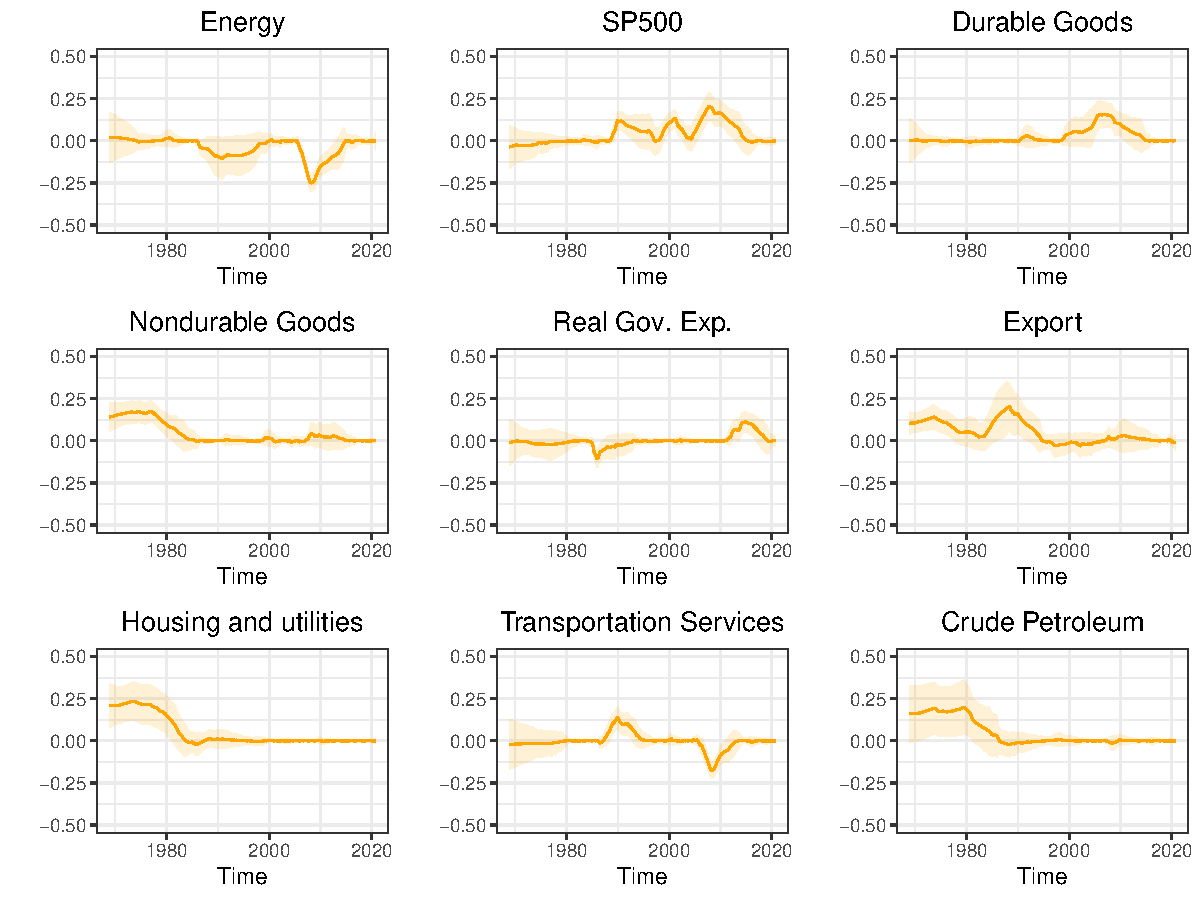
\includegraphics{Dynamic-Shrinkage-in-Bayesian-Structural-Time-Series-and-Vector-Autoregressive-Models_files/figure-latex/unnamed-chunk-10-1} 

}

\caption{Dynamic SSVS for BSTS model; smoothed estimates (yellow) with 95 percent credible intervals of some interesting regression coefficients.}\label{fig:unnamed-chunk-10}
\end{figure}

\newpage
\section{\small Unemployment rate nowcasting: list of predictors}

\begin{table}[H]

\caption{\label{tab:mytab101}List of Predictors}
\centering
\fontsize{8}{10}\selectfont
\begin{tabular}[t]{ccc}
\toprule
Source & Type & Label\\
\midrule
Yahoo & Contemporary & Dow Jones\\
FRED & Contemporary & NIKKEI225\\
FRED & Contemporary & NASDAQ100\\
FRED & Contemporary & SP500\\
FRED & One period lag & OILPRICEx\\
\addlinespace
FRED & One period lag & CPIAUSL\\
FRED & One period lag & INDPRO\\
FRED & One period lag & TWEXAFEGSMTHx\\
FRED & One period lag & RETAILx\\
FRED & One period lag & DPCERA3M086SBEA\\
\addlinespace
FRED & One period lag & CMRMTSPLx\\
FRED & One period lag & HOUST\\
FRED & One period lag & PAYEMS\\
FRED & One period lag & RPI\\
Google Trends & Contemporary & unemployment\\
\addlinespace
Google Trends & Contemporary & federal unemployment\\
Google Trends & Contemporary & compensation package\\
Google Trends & Contemporary & Unemployment compensation\\
Google Trends & Contemporary & Unemployment agency\\
Google Trends & Contemporary & employee benefits\\
\addlinespace
Google Trends & Contemporary & unemployment check\\
Google Trends & Contemporary & unemployment statistics\\
Google Trends & Contemporary & unemployment pa\\
Google Trends & Contemporary & unemployment office\\
Google Trends & Contemporary & unemployment insurance\\
\addlinespace
Google Trends & Contemporary & unemployment depression\\
Google Trends & Contemporary & unemployment benefits\\
Google Trends & Contemporary & subsidies\\
\bottomrule
\end{tabular}
\end{table}

\newpage
\section{BSTS model for Airpassengers data}

Here, a BSTS model with DSS priors is used to fit AirPassengers data.
The coefficients are correctly shrunk to zero and the model succeed in
capturing trend and seasonality.

\begin{figure}[H]

{\centering 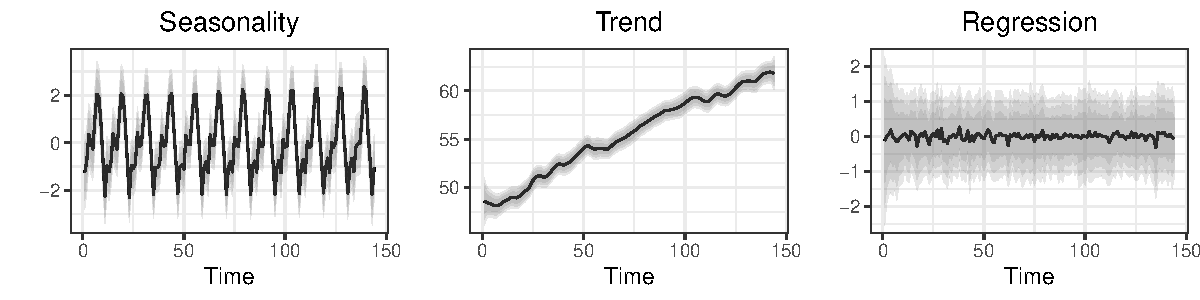
\includegraphics{Dynamic-Shrinkage-in-Bayesian-Structural-Time-Series-and-Vector-Autoregressive-Models_files/figure-latex/unnamed-chunk-11-1} 

}

\caption{Structural time series components. Point estimates (black) with credible intervals (gray).}\label{fig:unnamed-chunk-11}
\end{figure}

\begin{figure}[H]

{\centering 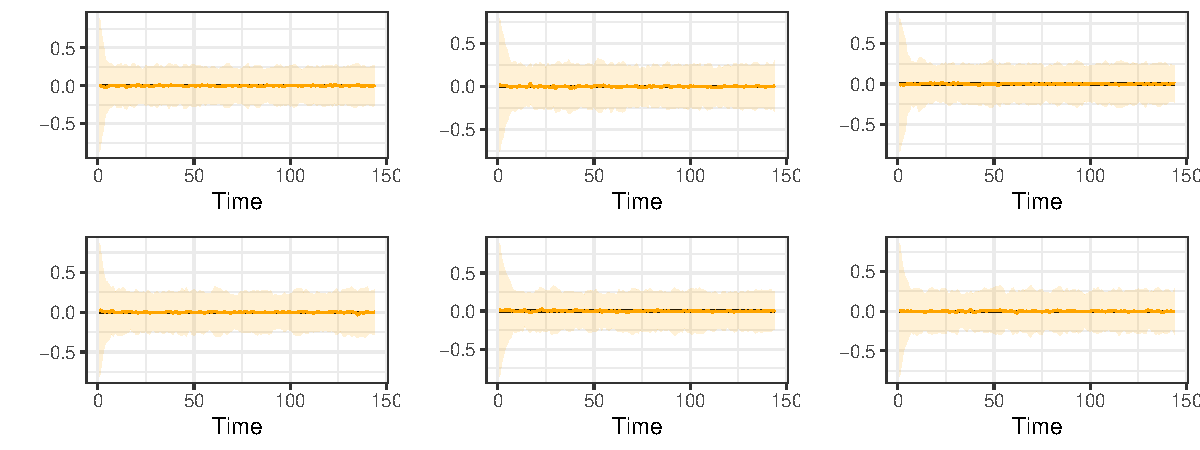
\includegraphics{Dynamic-Shrinkage-in-Bayesian-Structural-Time-Series-and-Vector-Autoregressive-Models_files/figure-latex/unnamed-chunk-12-1} 

}

\caption{Dynamic SSVS for BSTS model; true values of $\beta_{1:T, j}$, $j=1, \ldots, 6$, (black) and smoothed estimates with 95 percent credible intervals (yellow) of the first six regression coefficients. The coefficients are correctly shrunk to zero at every time.}\label{fig:unnamed-chunk-12}
\end{figure}

\begin{figure}[H]

{\centering 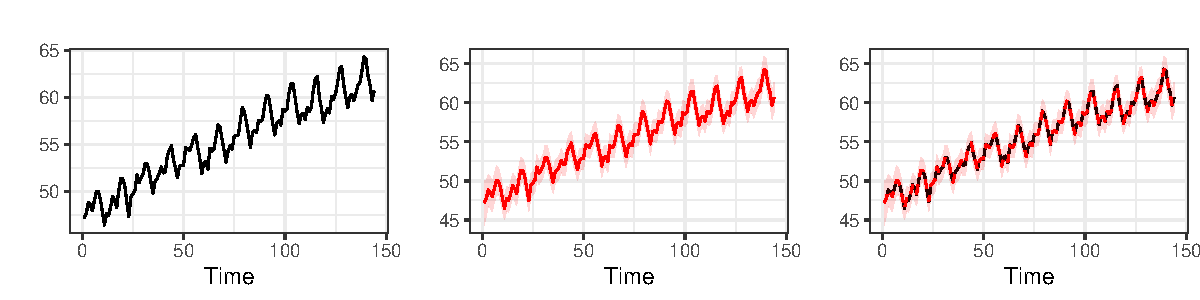
\includegraphics{Dynamic-Shrinkage-in-Bayesian-Structural-Time-Series-and-Vector-Autoregressive-Models_files/figure-latex/unnamed-chunk-13-1} 

}

\caption{Left panel: Airpassengers time series. Middle: fitted values with 95 credible intervals. Right panel: Airpassengers time series (black) and fitted values (red) with 95 credible intervals.}\label{fig:unnamed-chunk-13}
\end{figure}

\backmatter
\end{document}
